%%%%%%%%%%%%%%%%%%%%%%%%%%%%%%%%%%%%%%%%%
% Short Sectioned Assignment LaTeX Template Version 1.0 (5/5/12)
% This template has been downloaded from: http://www.LaTeXTemplates.com
% Original author:  Frits Wenneker (http://www.howtotex.com)
% License: CC BY-NC-SA 3.0 (http://creativecommons.org/licenses/by-nc-sa/3.0/)
%%%%%%%%%%%%%%%%%%%%%%%%%%%%%%%%%%%%%%%%%

% \documentclass[paper=a4, fontsize=11pt]{scrartcl} % A4 paper and 11pt font size
\documentclass[11pt, a4paper]{book}
\usepackage[T1]{fontenc} % Use 8-bit encoding that has 256 glyphs
\usepackage[utf8]{inputenc}
%\usepackage{mathptmx} % Use the Adobe Utopia font for the document - comment this line to return to the LaTeX default
\usepackage{listings} % para insertar código con formato similar al editor
\usepackage{color}  % si quieres usar colores en tu código
\usepackage[spanish, es-tabla]{babel} % Selecciona el español para palabras introducidas automáticamente, p.ej. "septiembre" en la fecha y especifica que se use la palabra Tabla en vez de Cuadro
\usepackage{url} % ,href} %para incluir URLs e hipervínculos dentro del texto (aunque hay que instalar href)
\usepackage{graphics,graphicx, float} %para incluir imágenes y colocarlas
\usepackage[gen]{eurosym} %para incluir el símbolo del euro
\usepackage{cite} %para incluir citas del archivo <nombre>.bib
\usepackage{enumerate}
\usepackage{enumitem}
\usepackage{hyperref}
\usepackage{graphicx}
\usepackage{tabularx}
\usepackage{booktabs}
\usepackage{textcomp}
\usepackage{adjustbox}
\usepackage{geometry}
\usepackage{amsmath}
\usepackage{amsthm} % Añadir este paquete
\usepackage{amsfonts}
\usepackage{amssymb}
\usepackage{subfigure}
\usepackage{textcomp}
\usepackage{longtable}
\usepackage{mwe} % Paquete necesario para la columna tipo 'm'
\usepackage{mathrsfs}
\usepackage{upquote}
\usepackage{mdframed}


\lstdefinestyle{lamportStyle}{
    language=Pascal,          % Usar configuración base de Pascal
    basicstyle=\ttfamily\small,
    numbers=left,
    numberstyle=\tiny,
    stepnumber=1,
    numbersep=5pt,
    tabsize=4,
    extendedchars=true,
    breaklines=true,
    keywordstyle=\color{blue},
    stringstyle=\color{orange}, % Cadena de caracteres en naranja
    commentstyle=\color{gray},
    frame=b,
    morekeywords={program, procedure, function, process, integer, real, char, boolean, string, begin, end, cobegin, coend, return},
    captionpos=b             % Posiciona el caption debajo del bloque de código   
}


\lstnewenvironment{BNFCode}{%
\lstset{
  language={}, % Vacío, no basarse en ningún lenguaje específico
  basicstyle=\ttfamily\color{black}, % Fuente de estilo básico en color negro
  morestring=[b]", % Define las cadenas de texto entre comillas dobles
  stringstyle=\color{red}, % Color rojo para cadenas de texto
  commentstyle=\color{orange}, % Color naranja para comentarios
  morecomment=[l]{\#}, % Define cómo se indican los comentarios
  keepspaces=true, % Mantiene los espacios
  breaklines=true, % Permite romper las líneas
  breakindent=1.5cm, % Sangría después de romper una línea
  breakatwhitespace=false, % Permite romper en cualquier espacio, no solo en espacios en blanco
  columns=fullflexible,
}
}{}

\lstdefinestyle{customflex}{
    language=C, % Flex se basa en C, así que esto debería resaltar la mayoría de la sintaxis correctamente
    basicstyle=\ttfamily\small,
    commentstyle=\color{gray},
    keywordstyle=\color{blue},
    numbers=left,
    breaklines=true,
    frame=single,
    captionpos=b
    \lstset{upquote=true}
}

\lstdefinestyle{myInlineCode}{
    basicstyle=\ttfamily,
    breaklines=true,  % Opcional: permite que el código se divida entre líneas
    keepspaces=true   % Opcional: conserva los espacios en el código
}


\usepackage[table,xcdraw]{xcolor}
\hypersetup{
	colorlinks=true,	% false: boxed links; true: colored links
	linkcolor=black,	% color of internal links
	urlcolor=cyan		% color of external links
}
%\renewcommand{\familydefault}{\sfdefault}
\usepackage{fancyhdr} % Custom headers and footers
\pagestyle{fancyplain} % Makes all pages in the document conform to the custom headers and footers
\fancyhead[L]{} % Empty left header
\fancyhead[C]{} % Empty center header
\fancyhead[R]{Daniel Pérez Ruiz} % My name
\fancyfoot[L]{} % Empty left footer
\fancyfoot[C]{} % Empty center footer
\fancyfoot[R]{\thepage} % Page numbering for right footer
%\renewcommand{\headrulewidth}{0pt} % Remove header underlines
\renewcommand{\footrulewidth}{0pt} % Remove footer underlines
\setlength{\headheight}{13.6pt} % Customize the height of the header

\usepackage{titlesec, blindtext, color}
\definecolor{gray75}{gray}{0.75}
\newcommand{\hsp}{\hspace{20pt}}
\titleformat{\chapter}[hang]{\Huge\bfseries}{\thechapter\hsp\textcolor{gray75}{|}\hsp}{0pt}{\Huge\bfseries}
\setcounter{secnumdepth}{4}
\usepackage[Lenny]{fncychap}


\newcolumntype{M}[1]{>{\centering\arraybackslash}m{#1}}

\renewcommand{\lstlistingname}{Programa}
\newcommand{\code}[1]{\lstinline[style=myInlineCode]!#1!}

\newtheorem{teorema}{Teorema}[section]
\newtheorem{definicion}[teorema]{Definición}
\newtheorem{corolario}[teorema]{Corolario}
\newtheorem{proposicion}[teorema]{Proposición}
\newtheorem{observacion}[teorema]{Observación}

\newcommand{\squareDiamond}{%
\tikz [x=1.2ex,y=1.2ex,line width=.1ex] \draw (0,0) -- (1,1) -- (0,2) -- (-1,1) -- cycle;}

\begin{document}

	% Plantilla portada UGR
	\begin{titlepage}
\newlength{\centeroffset}
\setlength{\centeroffset}{-0.5\oddsidemargin}
\addtolength{\centeroffset}{0.5\evensidemargin}
\thispagestyle{empty}

\noindent\hspace*{\centeroffset}\begin{minipage}{\textwidth}

\centering

\includegraphics[width=0.9\textwidth]{logos/logo_ugr.jpg}\\[1.4cm]

\textsc{ \Large TRABAJO FIN DE GRADO\\[0.2cm]}
\small \textsc{DOBLE GRADO EN INGENIERÍA INFORMÁTICA Y MATEMÁTICAS}\\[1cm]

{\Huge\bfseries Simulador de Sistemas Concurrentes y Distribuidos \\}
\noindent\rule[-1ex]{\textwidth}{3pt}\\[3.5ex]
\end{minipage}

\vspace{1.5cm}
\noindent\hspace*{\centeroffset}
\begin{minipage}{\textwidth}
\centering

\textbf{Autor}\\ {Daniel Pérez Ruiz}\\[2.5ex]
\textbf{Director}\\ {Carlos Ureña Almagro}\\[1.2cm]

\begin{figure}[H]
  \centering
  
\includegraphics[width=.3\textwidth]{logos/etsiit_logo.png}\hspace{0.2\textwidth}
  
\includegraphics[width=.2\textwidth]{logos/ciencias-logo.png}
\end{figure}
%
\includegraphics[width=0.3\textwidth]{logos/etsiit_logo.png}\\[0.1cm]
\textsc{Escuela Técnica Superior de Ingenierías Informática y de Telecomunicación}\\[0.1cm]
\textsc{Y}\\
\textsc{Facultad de Ciencias}\\
\textsc{---}\\
Granada, Junio de 2023
\end{minipage}
\end{titlepage}


	% Plantilla prefacio UGR
	\thispagestyle{empty}

\begin{center}
{\large\bfseries Simulador de Sistemas Concurrentes y Distribuidos. Lógica Temporal de Acciones }\\
\end{center}
\begin{center}
Daniel Pérez Ruiz\\
\end{center}

%\vspace{0.7cm}

\vspace{0.5cm}
\noindent\textbf{Palabras clave}: \textit{ágil, concurrencia, sistema, programa, lógica, instrucción, lenguaje, compilador, máquina virtual}
\vspace{0.7cm}

\noindent\textbf{Resumen}\\
Este trabajo se centra en el desarrollo de un compilador para un lenguaje de programación, nombrado Lamport en honor a Leslie Lamport y su influencia en el ámbito de los sistemas concurrentes y distribuidos, especialmente a través de su contribución con la Lógica Temporal de Acciones (TLA). Además este proyecto presenta un estudio detallado de TLA y un ejemplo práctico de su aplicación en la especificación de sistemas, proporcionando una perspectiva matemática y formal para la especificación y verificación de sistemas concurrentes en general. El objetivo principal, sin embargo, es la creación de una herramienta práctica que concretice los conceptos de concurrencia en una aplicación tangible y accesible para los usuarios.

El compilador de Lamport ha sido diseñado específicamente para simular sistemas concurrentes y distribuidos, permitiendo así a los usuarios interactuar directamente con las complejidades y retos inherentes a la programación en este campo. Desarrollado bajo una metodología ágil y utilizando las capacidades de los lenguajes C y C++, el compilador profundiza en la comprensión de aspectos clave como la sincronización de procesos o el manejo de bloqueos, a parte de ser un lenguaje totalmente funcional para programas secuenciales.

El trabajo también incluye una exploración de los principios fundamentales de los sistemas concurrentes y distribuidos, proporcionando el marco teórico esencial para comprender y utilizar eficazmente el compilador Lamport. Se examinan posibles ampliaciones y mejoras del compilador, incluyendo su eventual evolución hacia un modelo de Software as a Service (SaaS), la incorporación de mecanismos de sincronización más sofisticados y la expansión de la gramática del lenguaje.

\cleardoublepage

\begin{center}
	{\large\bfseries Concurrent and Distributed Systems Simulator. Temporal Logic of Actions}\\
\end{center}
\begin{center}
	Daniel Pérez Ruiz\\
\end{center}
\vspace{0.5cm}
\noindent\textbf{Keywords}: \textit{agile, concurrency, system, program, logic, instruction, language, compiler, virtual machine}
\vspace{0.7cm}

\noindent\textbf{Abstract}\\
This work focuses on the development of an compiler for a programming language, named Lamport in honor of Leslie Lamport and his influence in the field of concurrent and distributed systems, particularly through his contribution to Temporal Logic of Actions (TLA). Additionally, this project presents a detailed study of TLA and a practical example of its application in system specification, offering a mathematical and formal perspective for the specification and verification of concurrent systems in general. The main goal, however, is to create a practical tool that materializes the concepts of concurrency into a tangible and accessible application for users.

The Lamport compiler has been specifically designed to simulate concurrent and distributed systems, thus allowing users to directly interact with the complexities and challenges inherent in programming in this field. Developed under an agile methodology and utilizing the capabilities of C and C++ languages, the compiler deepens the understanding of key aspects such as process synchronization or deadlock handling, apart from being a fully functional language for sequential programs.

The work also includes an exploration of the fundamental principles of concurrent and distributed systems, providing the essential theoretical framework to effectively understand and use the Lamport compiler. Potential extensions and improvements of the compiler are examined, including its eventual evolution into a Software as a Service (SaaS) model, the incorporation of more sophisticated synchronization mechanisms, and the expansion of the language grammar.



\cleardoublepage

\thispagestyle{empty}

\noindent\rule[-1ex]{\textwidth}{2pt}\\[4.5ex]

D. \textbf{Tutora/e(s)}, Profesor(a) del ...

\vspace{0.5cm}

\textbf{Informo:}

\vspace{0.5cm}

Que el presente trabajo, titulado \textit{\textbf{Simulador de Sistemas Concurrentes y Distribuidos. Lógica Temporal de Acciones}},
ha sido realizado bajo mi supervisión por \textbf{Daniel Pérez Ruiz}, y autorizo la defensa de dicho trabajo ante el tribunal
que corresponda.

\vspace{0.5cm}

Y para que conste, expiden y firman el presente informe en Granada a Noviembre de 2023.

\vspace{1cm}

\textbf{El/la director(a)/es: }

\vspace{5cm}

\noindent \textbf{(nombre completo tutor/a/es)}

\chapter*{Agradecimientos}

Desde que era muy pequeño mi madre siempre me ha dicho que, si ves una mariposa blanca, eso es señal de suerte. Aunque no me caracterizo por ser una persona supersticiosa, siempre he convivido con esa inocencia cada vez que tenía ante mis ojos una de ellas, aleteando, al son de la libertad, iluminando en mí una sonrisa.

\vspace{0.2cm}

A lo largo de mi vida he tenido muchas ocasiones donde sentía que me habían abandonado. Y la realidad, es que siempre me han acompañado, aunque muchas veces no las viera. Ahí se encontraban, danzando al compás de todas las melodías y letras, de todas aquellas canciones que en tiempos pasados resonaron en mi cabeza.

\vspace{0.2cm} 

A mi madre, a mi hermana Irene, a mi padre. A mis amigos de toda una vida Adrián, Alberto, Elías, Juanmi, Juan, Rafa Aguilar y Rafa Barrales. A mis amigos de esta nueva vida Lucía, Martín, Mery, Jaime, Jose, Joseja y Pablo. No hay suficientes palabras en este mundo para describir lo inmensos que son. A mi amiga Candela, por haber por fin coincidido en este camino tras muchas historias y canciones, y que prometo recorrerlo bailando una vez más. A mi amiga Elena, por haber sido la mayor voz que me guió y me dio luz cuando no la había. A Coral, por haber venido casi al final con su deslumbrante forma de ser, brindándome un nuevo y prometedor comienzo. A mis dos grandes mentores: mi tutor, Carlos, por ser mi fuente de inspiración desde que coincidí con él; y JJ, la persona que me enseñó a cómo encontrarme si me perdía en el camino.

\vspace{0.2cm}
En este trabajo dejo atrás una muy buena parte de mi vida, donde cumplí el sueño de la infancia que me llevó hasta este mismo momento, el de descubrir y aprender todo lo \textit{immenso} que es el mundo de la informática, así como también lo es la vida misma. Esta parte de mí dejará de existir para siempre, pero ahora es mi turno de volar, al igual que todas las mariposas blancas que siempre estuvieron para mí.

\newpage
\vspace*{\fill}

\large
\noindent
$P := \textit{``Estás dispuesto a arriesgar.''}$
\newline
$Q := \textit{``Puedes crecer.''}$
\newline
$R := \textit{``Puedes dar lo mejor de ti.''}$
\newline
$S := \textit{``Puedes ser feliz.''}$
\newline
\newline

\noindent
\textit{Si} $\neg P \implies \neg Q$;
\newline
\textit{Si} $\neg Q \implies \neg R$;
\newline
\textit{Si} $\neg R \implies \neg S$;
\newline
\textit{Y si} $\neg S$, ¿qué te queda?
\newline



\vspace*{\fill}

	% Índice de contenidos
	\newpage
	\tableofcontents

	% Índice de imágenes y tablas
	\newpage
	\listoffigures

	% Si hay suficientes se incluirá dicho índice
	\listoftables 
	\newpage

	% Introducción 
	\chapter{\textbf{Introducción}}

\section{Motivación}
En el mundo actual, marcado por un avance tecnológico acelerado y una creciente digitalización, la importancia de los sistemas concurrentes y distribuidos se ha vuelto más evidente que nunca. Estos sistemas son fundamentales para el funcionamiento eficiente y óptimo de numerosas aplicaciones y servicios que forman la columna vertebral de la sociedad moderna. Desde el procesamiento de datos a gran escala hasta la computación en la nube, pasando por las redes de telecomunicaciones y la proliferación de la Internet de las Cosas (IoT), los sistemas concurrentes y distribuidos permiten el manejo y procesamiento simultáneo de enormes cantidades de información, asegurando la escalabilidad y la disponibilidad de los servicios.

En este entorno, la habilidad para diseñar, implementar y mantener sistemas que puedan manejar múltiples tareas de manera simultánea y distribuida es más que una habilidad técnica; es una necesidad vital. Con la integración creciente de la inteligencia artificial en diversos sectores, la eficiencia en la gestión de procesos concurrentes y la distribución efectiva de las cargas de trabajo no son solo deseables, sino esenciales para el avance y la innovación tecnológica. Además, la garantía de fiabilidad y seguridad en estos sistemas se convierte en un reto crítico, dado que cualquier fallo puede tener repercusiones significativas en un amplio espectro de actividades humanas.

En el grado de Ingeniería Informática de la Universidad de Granada, se dedica una asignatura completa al estudio de estos sistemas, denominada \textit{Sistemas Concurrentes y Distribuidos (SCD)}, donde se exploran tanto sus aspectos teóricos como prácticos. Esta asignatura no solo proporciona a los estudiantes una comprensión profunda de los fundamentos de los sistemas concurrentes y distribuidos, sino que también los introduce en el rigor matemático necesario para la verificación de sus propiedades utilizando un sistema lógico formal. Esta área de estudio es crucial, ya que asegura que los sistemas diseñados sean fiables, seguros y eficientes. Al enfrentarse a la complejidad inherente de estos sistemas, los alumnos aprenden a aplicar técnicas avanzadas de modelado y análisis.

La contrapartida es que su comprensión y aplicación práctica puede ser desafiante, especialmente para quienes se acercan por primera vez a la materia, y es por ello por lo que es crucial disponer de suficientes recursos y herramientas de apoyo que permitan alcanzar un aprendizaje íntegro y efectivo en este campo dinámico y en constante evolución.


\section{Objetivos del trabajo}
El propósito central de este proyecto es el desarrollo de un lenguaje de programación intuitivo y accesible , acompañado de un compilador específico, para facilitar el desarrollo y simulación de sistemas concurrentes. Este enfoque práctico busca proporcionar una alternativa a los lenguajes de programación de alto nivel convencionales, como C++, simplificando así el proceso de aprendizaje y enseñanza desde una perspectiva más accesible y transparente. Adicionalmente, este trabajo se adentra en un estudio sobre los fundamentos matemáticos subyacentes, centrándose en la Lógica Temporal de Acciones propuesta por Leslie Lamport. Este estudio es crucial para la especificación y verificación de los sistemas concurrentes, proporcionando una base teórica sólida que complementa y enriquece la comprensión práctica. Además, se explorarán los fundamentos detrás del procesamiento de lenguajes, esenciales para el diseño efectivo del lenguaje de programación propuesto. La combinación de estos enfoques prácticos y teóricos no solo busca lograr un entendimiento integral de los sistemas concurrentes y distribuidos, sino también fomentar una sinergia entre la teoría matemática y la aplicación práctica en el campo de la informática. A modo de resumen, los objetivos a cumplimentar son:

\begin{itemize}
    \item Desarrollar un marco teórico que abarque los conceptos clave de los sistemas concurrentes y distribuidos, proporcionando una comprensión clara y detallada de su funcionamiento, principios y desafíos. Incluir un estudio de los fundamentos matemáticos de las lógicas formales que sustentan las bases de la Lógica Temporal de Acciones, haciendo énfasis en su aplicación para la especificación y verificación de sistemas concurrentes. Se abordarán los principios fundamentales de la lógica y del tiempo, explorando cómo se integran y aplican en el contexto de la computación concurrente y distribuida.
    \item Llevar a cabo el desarrollo de un proyecto de software desde sus inicios utilizando metodologías de desarrollo ágil, poniendo el foco siempre en los clientes, que son las personas interesadas en el producto y quienes verdaderamente guían a un equipo hacia su progreso.
    \item Realizar un análisis y descripción detallada del lenguaje de programación a desarrollar, denominado \textit{Lamport}, tomando como punto de partida la sintaxis de los ejemplos de pseudocódigo de la asignatura \textit{Sistemas Concurrentes y Distribuidos} del grado de Ingeniería Informática de la Universidad de Granada.
    \item Implementar un compilador del código descrito, teniendo en cuenta las fases de análisis y optimización. Posteriormente, modelar una máquina virtual capaz de interpretar directamente el código generado, mostrando la ejecución resultante de las instrucciones al usuario, además de otorgarle transparencia en los sucesivos eventos que han ido ocurriendo por dentro, con el objetivo de garantizar un aprendizaje integral.
\end{itemize}

\section{Contenido del documento}\label{section:documentInfo}
Este documento está estructurado en 5 partes principales, cada una enfocada en aspectos distintos y fundamentales del proyecto. A continuación, se detalla el contenido de cada parte:

\begin{itemize}
    \item \textbf{Parte 1: Introducción y Motivación - El Origen y Propósito del Proyecto}. Esta sección explora la motivación detrás del proyecto, el problema que busca resolver y la metodología aplicada. Se detalla la planificación y evolución del proyecto, incluyendo un enlace al repositorio de GitHub para seguimiento práctico. Comprende los capítulos 1, 2 y 3.
    \item \textbf{Parte 2: Estado del Arte - El Contexto y la Relevancia Actual}. Se presenta un contexto histórico sobre la evolución de los sistemas concurrentes y distribuidos, destacando la contribución única del proyecto a esta área. Comprende el capítulo 4.
    \item \textbf{Parte 3: Fundamentos Teóricos y Matemáticos - La Base Conceptual del Proyecto}. Se realiza un análisis teórico completo de los sistemas concurrentes y distribuidos, abarcando desde la teoría matemática de sistemas lógicos formales, hasta los aspectos necesarios para la implementación práctica. Comprende los capítulos 5, 6 y 7.
    \item \textbf{Parte 4: Diseño e Implementación del Lenguaje de Programación Lamport - La Construcción de una Herramienta Innovadora}. Se tratan los aspectos técnicos del lenguaje Lamport, desde su diseño hasta la compilación, resaltando la importancia de los ejemplos prácticos para demostrar su eficacia. Comprende los capítulos 8, 9, 10, 11.
    \item \textbf{Parte 5: Conclusiones - Reflexiones y Perspectivas Futuras}. Se ofrecen reflexiones finales sobre los temas tratados y se sugieren direcciones futuras para la herramienta desarrollada, resumiendo los logros y aprendizajes clave del proyecto. Comprende el capítulo 12.

    
\end{itemize}

	% Descripción del problema y hasta donde se llega
	\chapter{\textbf{Descripción del problema}}\label{chapter:problema}

Este trabajo busca responder a las dos siguientes preguntas: ¿cómo se puede optimizar, a nivel teórico y práctico, el estudio e implementación de los conceptos de diseño y desarrollo de programas concurrentes? ¿Qué métodos existen para verificar formalmente las propiedades de dichos programas? Aunque existen innumerables maneras de abordar estos desafíos planteados, sólo el uso de una metodología clara, segura y correcta resulta verdaderamente adecuado.

\section{Metodología: Desarrollo Ágil}
La siguiente frase de Siegbert Tarrasch, quien fue uno de los mejores jugadores de ajedrez de todos los tiempos, es digna de mención: \textit{"La belleza de un movimiento no se refleja sólo en su apariencia, sino en el pensamiento detrás de él"}. No basta con tener acciones o hechos; es esencial que detrás de ellos exista una \textbf{idea}, un \textbf{problema} o simplemente una \textbf{pregunta} que sirva de base para construir paso a paso todos los objetivos que se deseen alcanzar. Del mismo modo que en el ajedrez cada movimiento es estratégico y sigue una lógica o un plan, en un proyecto que precise de la ingeniería informática cada paso dado debe estar fundamentado y orientado hacia la resolución del problema central.

En un proyecto de ingeniería informática, es esencial identificar claramente el problema que se desea resolver y la razón subyacente. Una vez definido, es importante garantizar que el proyecto en cuestión realmente aborde dicho problema \cite{jj-agile-objetivos}. La estrategia más efectiva consiste en dividir el problema en segmentos más manejables, a los que podemos referirnos como \textit{objetivos}. La recurrente mención de la palabra \textbf{"problema"} subraya su importancia central en la metodología, pues no se espera otra cosa que \textit{solucionar dicho problema}.

El desarrollo ágil surgió tras la redacción y firma del \textit{Manifiesto por el Desarrollo Ágil de Software} \cite{agile-manifest} por diecisiete expertos en programación. Con el término \textit{ágil} no se alude únicamente a una metodología para el desarrollo de proyectos que precisan de rapidez y flexibilidad, sino también una filosofía que implica una forma distinta de trabajar y de organizarse a la que predominaba anteriormente, denominada \textit{metodología en cascada}. Así pues, por \textit{ágil} se entiende una mentalidad que se aplica a todo el ciclo de vida del desarrollo de software, centrada en el cliente y en la mejora continua de productos mínimamente viables cada vez más complejos \cite{jj-agile-manifesto}.

Todo proyecto debe nacer de una motivación inicial, respondiendo a interrogantes como \textit{``por qué''}, \textit{``para qué''}, \textit{``para quién''} y \textit{``cómo''}. Si bien todas estas cuestiones son importantes, la penúltima destaca particularmente porque el éxito radica en satisfacer los \textit{deseos} y \textit{necesidades} de un grupo específico de clientes o usuarios unidos por una característica común: un \textit{problema}. 
Resolverlo implica practicar la \textbf{empatía} con ellos, esforzándose por comprender profundamente sus necesidades y determinar cómo satisfacerlas de manera óptima, aportando \textbf{valor} con los recursos disponibles. Las entrevistas personales o el seguimiento de las tendencias actuales pueden proporcionar la perspectiva adecuada.

De ahí surgen las \textbf{Historias de Usuario}, que proporcionan una explicación informal desde el punto de vista del usuario final y siempre situadas dentro del dominio del problema, de una funcionalidad del software que principalmente tendrá que ver con la lógica de negocio del proyecto.\cite{jj-design-thinking}. Una vez definidas, lo que queda es especificar los productos que se entregarán a los clientes, descritos a través de una secuencia de \textbf{hitos} o \textbf{milestones}. La esencia del desarrollo ágil radica en efectuar mejoras iterativas sobre el producto, contando siempre con la aprobación del usuario. En consecuencia, el avance del proyecto no es lineal, sino un proceso incremental.

En resumen, el desarrollo ágil supuso un gran cambio en el paradigma de la organización y planificación de proyectos de ingeniería informática, colocando al usuario y sus necesidades en el centro del proceso, guiando cada paso a través de la empatía y una comprensión profunda del problema. Con herramientas como las Historias de Usuario y la propia naturaleza de la metodología basada en un proceso iterativo e incremental, se busca proporcionar soluciones más adaptadas y flexibles de la ingeniería moderna, puesto que las necesidades de los clientes pueden ir variando con el tiempo. Es un enfoque que valora la colaboración y la resiliencia, con el objetivo de siempre aportar valor, abordando así los actuales y futuros desafíos del mundo tecnológico.

\section{Clientes}
Tras haber explorado la esencia del desarrollo ágil y su prioridad hacia el usuario y sus deseos, ahora se profundizará en el concepto de \textbf{cliente}. Los problemas y expectativas de los clientes o usuarios son lo que impulsan las decisiones y acciones del equipo de desarrollo. 

Para identificar y comprender los distintos usuarios del compilador de código, se empleó una metodología centrada en las personas. Se llevaron a cabo entrevistas individuales a dos grupos de personas \textit{reales} \footnote{Aunque no es estrictamente necesario utilizar personas reales para el análisis de un problema en el desarrollo de un proyecto, hacerlo añade una dimensión \textit{humana} que, en mi experiencia con otros proyectos, aumenta considerablemente las probabilidades de éxito.} vinculadas a la asignatura de \textit{Sistemas Concurrentes y Distribuidos}: estudiantes y profesorado. A ambos grupos se les formuló una serie de preguntas, que se presentan a continuación.

\noindent
Las preguntas planteadas al alumnado de la asignatura fueron:
\begin{itemize}
    \item \textit{¿Te resulta complicado entender los conceptos o fundamentos teóricos de la asignatura?}
    \item \textit{¿Eres capaz de resolver un problema que involucre concurrencia sin programarlo explícitamente?}
    \item \textit{¿Notas una diferencia significativa entre la teoría y práctica de la asignatura?}
    \item \textit{¿Crees que programar en el pseudocódigo específico de la asignatura te facilitaría su aprendizaje?}
\end{itemize}

\noindent
Las preguntas planteadas al profesorado fueron:
\begin{itemize}
    \item \textit{¿Consideras que la asignatura es difícil para los estudiantes?}
    \item \textit{¿Ves una diferencia significativa entre la teoría y la práctica de la asignatura?}
    \item \textit{¿Piensas que programar en el pseudocódigo específico de la asignatura ayudaría a los alumnos durante el curso? ¿Facilitaría tu labor docente al explicar los conceptos?}
\end{itemize}

Las dos últimas preguntas de cada grupo son similares, buscando comprobar la concordancia entre ambos puntos de vista. Las respuestas de los estudiantes indican que, aunque la asignatura posee una complejidad relativa en comparación con otras del grado, los conceptos en sí no son difíciles de asimilar. La verdadera barrera surge al aplicar estos conceptos en el diseño de sistemas concurrentes o al tratar de resolver problemas sin recurrir a un lenguaje de alto nivel, como C++. Los estudiantes generalmente consideran que se desenvuelven mejor en la práctica que en la teoría. Esta preferencia puede deberse a su familiaridad con el enfoque práctico adoptado en los primeros años del grado, con este lenguaje en particular. Por tanto, la respuesta a la última pregunta suele ser un \textit{sí} rotundo.

El profesorado, por su parte, no ve a su asignatura como particularmente complicada y no percibe una gran diferencia entre la teoría y práctica. Sin embargo, muestran empatía hacia los estudiantes, entendiendo que ellos puedan sentir una mayor complejidad. Coinciden en que disponer de un lenguaje de programación con la sintaxis propuesta en la asignatura podría facilitar una enseñanza más didáctica y accesible.

Con esta información no sólo obtenemos la motivación mencionada en la sección anterior, sino que también podemos identificar a los dos usuarios potenciales del compilador a desarrollar. A continuación, se describirá detalladamente el perfil de cada tipo de usuario.

\subsection{Tipo de usuario 1: Estudiante}
Se proporciona una descripción detallada de un perfil de usuario de tipo estudiante:

\begin{description}
    \item[Nombre:] Luis Martínez
    \item[Características Demográficas:] \hfill
        \begin{itemize}
            \item Edad: 19 años.
            \item Estudiante universitario de ingeniería informática, actualmente cursando la asignatura de \textit{Sistemas Concurrentes y Distribuidos}.
        \end{itemize}
    \item[Necesidades y Objetivos:] Luis aspira a aprobar la asignatura de \textit{Sistemas Concurrentes y Distribuidos} para avanzar en sus estudios. Además, busca comprender conceptos que sean importantes en futuras asignaturas relacionadas con su grado.
    
    \item[Habilidades Técnicas:] Posee habilidades de programación de nivel principiante a intermedio. Es probable que esta sea su primera experiencia con la implementación de programas no secuenciales.
    
    \item[Escenarios de Uso Comunes:] Luis utiliza el compilador para validar ejercicios específicos de la clase sobre sincronización de hebras o procesos.
    
    \item[Limitaciones:] Aunque Luis se siente cómodo programando en lenguajes de alto nivel como C++, enfrenta dificultades al comprender la sintaxis del pseudocódigo. Esto puede dificultar su capacidad para traducir rápidamente los conceptos teóricos en implementaciones prácticas utilizando pseudocódigo.
    
    \item[Expectativas:] Espera poder disponer de un lenguaje de pseudocódigo funcional, pudiendo añadir comentarios explicativos a cada línea de código para facilitar su comprensión. Además, desea que las ejecuciones de los programas se visualicen de forma clara, permitiéndole seguir el proceso paso a paso para consolidar su entendimiento de los conceptos teóricos.
\end{description}

\subsection{Tipo de usuario 2: Profesor}
Se proporciona una descripción detallada de un posible perfil de usuario de tipo profesor:

\begin{description}
    \item[Nombre:] Laura Ruiz
    \item[Características Demográficas:] \hfill
        \begin{itemize}
            \item Edad: 42 años.
            \item Profesora titular de la asignatura \textit{Sistemas Concurrentes y Distribuidos} en la facultad de Ingeniería Informática.
            \item Más de 10 años de experiencia docente en el campo de la informática.
        \end{itemize}
    \item[Necesidades y Objetivos:] Desea que sus estudiantes comprendan a fondo los conceptos y aplicaciones de los sistemas concurrentes y distribuidos. Busca herramientas y métodos que puedan hacer que la enseñanza sea más interactiva y efectiva.
    
    \item[Habilidades Técnicas:] Amplios conocimientos en programación, sistemas concurrentes, y pedagogía. Familiarizada con varios lenguajes de programación, incluido C++.
    
    \item[Escenarios de Uso Comunes:] Utilizar el compilador para demostrar ejemplos en clase, proponer ejercicios prácticos a los estudiantes y evaluar soluciones propuestas por ellos. Puede usarlo también para simular escenarios concurrentes y mostrar visualmente a los estudiantes cómo funcionan.
    
    \item[Limitaciones:] Prefiere que la herramienta tenga una interfaz amigable y sea intuitiva, ya que no desea invertir mucho tiempo en aprender a usarla. 
    
    \item[Expectativas:] Espera que el compilador permita explicaciones paso a paso y que pueda integrarse fácilmente con otros recursos didácticos. Le interesa que el pseudocódigo esté alineado con el contenido teórico de la asignatura, facilitando la transición entre teoría y práctica.
\end{description}

\newpage

\section{Historias de Usuario}

A través de las \textbf{Historias de Usuario}, se busca no solo definir qué es lo que el software debe hacer, sino también por qué es relevante hacerlo y cuál es el valor que se ofrece al usuario final. A continuación, se presentarán las Historias de Usuario identificadas para el desarrollo del compilador de código y cómo estas sientan las bases para los \textit{milestones} y Productos Mínimamente Viables del proyecto.

\begin{itemize}
    \item \textbf{Historia de usuario 1 (HU1):} Como estudiante de la asignatura, Luis quiere disponer de un compilador para escribir y ejecutar programas en el lenguaje de pseudocódigo propuesto en las transparencias, con el objetivo de practicar y verificar el funcionamiento de las soluciones a los ejercicios planteados.
    \item \textbf{Historia de usuario 2 (HU2):} Como profesora de la asignatura, Laura quiere contar con un compilador del lenguaje de las transparencias para poder explicar de forma más práctica los conceptos teóricos sin requerir un lenguaje de programación estándar como puede ser C++ o Java, además de poder revisar y analizar el código fuente desarrollado eventualmente por sus alumnos, y proporcionarles retroalimentación personalizada a los mismos.
\end{itemize}

\section{Milestones del proyecto: Productos Mínimamente Viables (PMV)}

Siguiendo la línea de las \textit{Historias de Usuario} y la importancia de establecer una comunicación efectiva con el usuario final, es el momento de definir productos entregables concretos que materialicen estas historias en el transcurso del desarrollo, que comúnmente se denomina \textbf{Productos Mínimamente Viables (PMV)}. Están diseñados no solo como representaciones tangibles del progreso, sino también como puntos de revisión donde se puede evaluar y adaptar el proyecto basándose en la retroalimentación aportada o por el propio cliente o por otro equipo de desarrollo. Los \textbf{milestones} o \textbf{hitos} sirven para secuenciar y organizar estos PMV en el ámbito del desarrollo ágil. A continuación, se enumeran los \textit{milestones} establecidos para este proyecto y cómo cada uno aporta al objetivo final del compilador de código.

\subsection{Milestone 0: Infraestructura del proyecto y definición del lenguaje.}\label{subsection:PMV0}
El primer hito del proyecto se centra en establecer una base sólida para su desarrollo. Comienza con una definición clara del problema, obtenida a través de entrevistas con usuarios potenciales, y la formulación detallada de este problema junto con la elaboración de las historias de usuario. Paralelamente, se lleva a cabo un estudio exhaustivo del lenguaje de pseudocódigo utilizado en la asignatura de Sistemas Concurrentes y Distribuidos, analizando sus componentes y definiendo su gramática utilizando la notación de Backus-Naur. En el aspecto técnico, se seleccionan cuidadosamente herramientas esenciales para el proyecto, incluyendo el lenguaje de programación para el compilador, un sistema de control de versiones, gestores de dependencias y tareas, herramientas de linting y ejecución de tests. Además, se configuran estas herramientas para garantizar la gestión eficiente de las dependencias, la calidad del código, y la automatización de tareas repetitivas como la compilación y la ejecución de tests.

\subsection{Milestone 1: Implementación del Analizador Léxico.}\label{subsection:PMV1}
Este hito se dedica a la construcción y validación del analizador léxico, una etapa crucial en el proceso de interpretación de cualquier lenguaje de programación. El foco principal es desarrollar una herramienta capaz de convertir una cadena de entrada en una serie de tokens identificables, que serán fundamentales para las etapas posteriores del compilador. Para lograrlo, se considera una herramienta generadora de analizadores léxicos que se ajuste a las especificaciones del lenguaje y las necesidades del proyecto. A continuación, se definen los tokens del lenguaje, incluyendo palabras reservadas, identificadores y operadores, junto con sus patrones de reconocimiento. La implementación del analizador léxico se realiza utilizando esta herramienta, asegurando su capacidad para reconocer y clasificar correctamente cada token. Además, se establece una tarea de generación del analizador léxico para facilitar su integración con el sistema, así como una tarea de limpieza de código objeto y ficheros compilados para mantener la organización y eficiencia del proyecto.

\subsection{Milestone 2: Implementación del Analizador Sintáctico.}\label{subsection:PMV2}
El segundo hito se enfoca en el diseño e implementación del analizador sintáctico, esencial para verificar la estructura correcta del código fuente en el lenguaje de pseudocódigo, según la gramática definida previamente. Este proceso incluye la definición de operadores, su aridad, asociatividad y orden de precedencia. Se selecciona una herramienta generadora de analizadores sintácticos y se ajusta la gramática del lenguaje. Tras implementar el analizador, se establece una estrategia para la recuperación de errores sintácticos y se define una tarea para su generación/compilación. Paralelamente, se desarrolla el Árbol Sintáctico Abstracto (AST), integrándolo con el analizador y definiendo una módulo para su gestión. Se implementan estructuras y funciones para la gestión de errores sintácticos y su integración con el analizador. Además, se llevan a cabo pruebas de integración y se desarrolla el programa principal del compilador, permitiendo la lectura de ficheros de texto plano, el procesamiento del pseudocódigo, la impresión del AST o los errores sintácticos detectados.

\subsection{Milestone 3: Implementación del Analizador Semántico.}\label{subsection:PMV3}
Este milestone se enfoca en el diseño e implementación del analizador semántico, una fase crítica que garantiza que el código fuente en el lenguaje de pseudocódigo no solo esté estructuralmente correcto (como asegura el analizador sintáctico) sino que también posea un significado lógico y coherente. El proceso incluye la descripción semántica del lenguaje y la implementación de una Tabla de Símbolos para gestionar identificadores y sus propiedades. Se desarrollan algoritmos clave para la resolución de nombres y la comprobación de tipos, asegurando que cada identificador se declare correctamente y que las operaciones entre diferentes tipos de variables sean válidas. Se establece una tarea de compilación para el módulo Analizador Semántico, facilitando su integración con otros componentes del compilador. Además, se realizan pruebas de integración para validar su funcionamiento en diversos escenarios de código. Se implementan estructuras y funciones para la gestión y reporte de errores semánticos, integrando el módulo de errores con el analizador para proporcionar retroalimentación específica al usuario. Finalmente, se habilita la función de análisis semántico dentro del flujo del compilador, proporcionando mensajes claros sobre el éxito del análisis o los errores detectados.

\subsection{Milestone 4: Análisis e implementación de la fase de generación de código intermedio.}\label{subsection:PMV4}
El cuarto hito se centra en el diseño e implementación de la fase de generación de código intermedio, un proceso clave que convierte el árbol de análisis sintáctico en una representación intermedia más cercana al código de máquina. Esta fase comienza con la selección de una representación intermedia adecuada para el lenguaje desarrollado y la definición de sus instrucciones, especificando operandos y usos. Se desarrolla un generador de código intermedio, con tablas para mapear variables, etiquetas y literales, y controladores para la generación y optimización del código. Paralelamente, se implementa un manejador de registros de eventos para documentar y ofrecer transparencia sobre las fases de análisis del compilador, incluyendo el análisis sintáctico, semántico y la generación del código intermedio. Se llevan a cabo pruebas de integración para asegurar la funcionalidad del módulo de generación de código intermedio y se habilita su función dentro del flujo general del compilador, junto con la generación de ficheros de registro de eventos para las distintas fases de análisis.


\subsection{Milestone 5: Análisis e implementación del compilador de código intermedio o máquina virtual}\label{subsection:PMV5}
El quinto hito del proyecto se centra en el diseño e implementación de un compilador para el código intermedio generado en las fases anteriores, que actúa como una máquina virtual. Esta máquina virtual está diseñada para ejecutar la representación intermedia, creando un entorno controlado que simula las operaciones de una máquina real de forma abstracta y agnóstica a la arquitectura del hardware. Para lograrlo, se implementan varios componentes clave: un esquema de traducción de direcciones virtuales a físicas, una abstracción de bloque de memoria, la memoria de la máquina virtual, un vector de registros de CPU, la CPU de la máquina virtual y un sistema operativo simulado para la máquina. Además, se aborda el tratamiento de excepciones como ZeroDivision e IndexOutOfBounds. La finalización de este milestone incluye realizar pruebas de integración exhaustivas para asegurar la funcionalidad y la integración adecuada de la máquina virtual con el resto del sistema.

\subsection{Milestone 6: Desarrollo teórico. Fundamentos matemáticos y tecnológicos}\label{subsection:PMV6}
El sexto milestone se enfoca en el desarrollo teórico, introduciendo los conceptos fundamentales de los sistemas concurrentes y distribuidos y realizando un estudio detallado de las lógicas formales, con énfasis en la Lógica Temporal de Acciones. Este enfoque teórico está diseñado para proporcionar una comprensión profunda de las bases matemáticas y lógicas necesarias para la verificación formal de sistemas concurrentes. Se explora la Lógica Temporal de Acciones, desarrollada por Leslie Lamport, para entender cómo se puede aplicar en el contexto de la verificación y el aseguramiento de la confiabilidad y coherencia en los sistemas concurrentes. El estudio se extiende a la explicación de cómo estos principios teóricos se integran y aplican en la práctica, resaltando su relevancia en el diseño, análisis y evaluación de sistemas que requieren una sincronización y coordinación efectivas. Este milestone no solo fortalece la base teórica del proyecto, sino que también proporciona a los usuarios las herramientas y conocimientos necesarios para abordar desafíos complejos en el campo de los sistemas concurrentes y distribuidos, preparándolos para enfrentar y resolver problemas prácticos con una sólida comprensión teórica.



	% Estado del arte
	\chapter{\textbf{Estado del arte}}
La \textit{programación concurrente} sienta sus bases en la década de los 1960 con la aparición de los sistemas operativos multiprogramación, que pretendían resolver uno de los problemas más críticos que se daban en aquella época: el uso eficiente de los recursos hardware. Anteriormente, la CPU ejecutaba sólo un programa a la vez, quedando inactiva si se producían operaciones de entrada/salida subutilizando sus recursos, produciendo como resultado un rendimiento deficiente. Con la multiprogramación, varios programas podían residir simultáneamente en la memoria principal, permitiendo a la CPU ejecutar otro programa diferente mientras se gestionaba una interrupción de E/S. Esta gestión se facilitó gracias a la invención de los ``canales'', controladores de dispositivos que operaban de forma independiente. Esta revolucionaria técnica tuvo un gran impacto en algunos sistemas informáticos que se desarrollaban por aquel entonces, como es el caso de los ``mainframes'' \cite{TecnologiaInformaticaMainframe}.


La programación concurrente fue inicialmente motivo de preocupación de los diseñadores de sistemas operativos. Al final de esta década de 1960, los diseñadores de hardware desarrollaron máquinas multiprocesador, que supusieron todo un reto para la implementación de nuevos sistemas operativos adaptados a estos recursos, pero también definió una nueva oportunidad para que los desarrolladores de aplicaciones pudieran emerger y posicionarse en el mercado laboral como una profesión con grandes expectativas a futuro.



El primer gran reto de esta nueva técnica de programación fue resolver lo que se denomina como: \textit{el problema de la sección crítica} \cite{GeeksForGeeksCriticalSection}. Este desafío central se refiere al desarrollo de algoritmos efectivos para la sincronización de procesos concurrentes que requieren acceder a un recurso compartido. La importancia de resolver este problema radica en la necesidad de evitar conflictos y garantizar la coherencia de los datos cuando múltiples procesos intentan leer o modificar el mismo recurso simultáneamente. La correcta gestión de la sección crítica es crucial para asegurar que los sistemas concurrentes funcionen de manera fiable y eficiente. Para entender mejor y modelar este reto, se plantearon problemas teóricos como \textit{la cena de los filósofos} \cite{brosgol1996dining}, \textit{lectores y escritores} \cite{nithyasrikannathalreaders}, \textit{el barbero durmiente} \cite{SariSleepingBarber} o el \textit{problema de los fumadores} \cite{MTUSmokerProblem}.


Estos escenarios anteriormente mencionados han sido ampliamente estudiados, generando miles de artículos que proponen soluciones, mejoras, debates y nuevas implementaciones de primitivas de sincronización como los semáforos o los monitores, que simplificaban la tarea del programador. Paralelamente, los lenguajes de programación de alto nivel estaban proliferando y evolucionando. Un ejemplo notable es Simula \cite{Sklenar1997OOPSimula}, desarrollado en la década de 1960 por Ole-Johan Dahl y Kristen Nygaard. Considerado uno de los primeros lenguajes orientados a objetos, Simula también introdujo conceptos fundamentales que influirían en la simulación de concurrencia, aunque su principal aporte fue establecer las bases para la programación orientada a objetos, un paradigma que tendría un impacto significativo en el desarrollo futuro de lenguajes y técnicas de programación concurrente.


Al final de la década de 1970 y principios de 1980, el surgimiento de redes de ordenadores como ARPANET, que facilitó la computación en áreas amplias, y el desarrollo de tecnologías como Ethernet para redes locales, marcó el comienzo de una nueva era en la informática. Estos avances no solo transformaron la forma en que las computadoras se conectaban y comunicaban entre sí, sino que también ampliaron significativamente el campo de la programación concurrente. Mientras la programación concurrente se enfoca en gestionar múltiples procesos dentro de un mismo sistema, las redes de computadoras introdujeron el desafío de coordinar procesos que se ejecutan en diferentes máquinas físicas. Esto dio origen a lo que se conoce como \textit{programación distribuida}, un enfoque que extendía los principios de la programación concurrente a sistemas distribuidos cuya esencia reside en que los procesos interactúan entre ellos a través del envío de mensajes en vez de escribir y leer variables compartidas.


A medida que la programación concurrente y distribuida ganaban relevancia en la década de 1980 y 1990, su integración en los lenguajes de programación de alto nivel comenzó a materializarse de manera significativa. Un hito notable en este desarrollo fue el lenguaje de programación Ada \cite{burns1998concurrency}, introducido en 1983. Diseñado originalmente para satisfacer las exigentes necesidades de los proyectos de defensa y sistemas en tiempo real, Ada se destacó por su soporte nativo para la programación concurrente. Su enfoque en la seguridad, la fiabilidad y la gestión sofisticada de tareas concurrentes lo convirtió en una herramienta fundamental para aplicaciones críticas. Posteriormente, en la década de 1990, Java emergió como un lenguaje de programación influyente, llevando la programación concurrente a un público más amplio. Con su API de concurrencia, Java simplificó la gestión de hilos y procesos concurrentes, haciendo que la programación de este tipo fuera más accesible y manejable para los desarrolladores. Esta API proporcionó un conjunto robusto de herramientas y estructuras para el manejo eficiente de tareas concurrentes y sistemas distribuidos, reflejando la creciente demanda de aplicaciones que operaban en entornos de red y web. La evolución de la programación concurrente en Ada y Java no solo demuestra cómo se han adaptado los lenguajes de programación a desafíos técnicos complejos, sino también cómo han evolucionado para satisfacer las necesidades de aplicaciones modernas en diversos entornos de computación. Pero no solo los lenguajes en sí, sino también las herramientas para crearlos, evolucionaron significativamente durante este periodo. El desarrollo de herramientas avanzadas para generar compiladores facilitó la creación de lenguajes de programación más sofisticados, especialmente aquellos diseñados para la programación concurrente y distribuida. Estas herramientas permitieron a los diseñadores de lenguajes experimentar con nuevas construcciones y paradigmas, facilitando el desarrollo de lenguajes que pudieran manejar de manera más eficiente y segura las complejidades inherentes a la concurrencia y la distribución. 


Sin embargo, cada vez que se implementaban mejoras en la programación concurrente y distribuida, con nuevas ideas y hardware, la complejidad de los programas aumentaba exponencialmente. Esto llevó a un incremento similar en la dificultad de verificar su funcionamiento correcto. Poco después del origen de este modelo de programación, surgió la necesidad de introducir formalismos capaces de demostrar rigurosamente que un programa concurrente posee ciertas propiedades. En este contexto, las herramientas matemáticas formales, especialmente la lógica temporal, se convirtieron en indispensables. La lógica temporal, que se ocupa de los aspectos temporales del razonamiento en la lógica matemática, permitía especificar y razonar sobre el comportamiento de los programas a lo largo del tiempo, asegurando propiedades como la seguridad (nunca ocurrirá nada malo) y la vivacidad (realmente sucede algo bueno) en sistemas concurrentes.


Un desarrollo particularmente significativo en el campo de la verificación de sistemas fue la Lógica Temporal de Acciones (TLA) de Leslie Lamport, cuya vida y carrera han sido tan influyentes como sus logros académicos \footnote{Lamport fue también el desarrollador inicial de \LaTeX, el sistema de composición de documentos utilizado para redactar este informe. A lo largo de su carrera, ha sido galardonado con numerosos premios, incluyendo el prestigioso Premio Turing, por sus contribuciones a la informática teórica. Sus trabajos, incluyendo la TLA, han influenciado tanto la teoría como la práctica en el diseño y verificación de sistemas distribuidos y concurrentes.}. Nacido en 1941 en Nueva York, Lamport demostró un interés temprano en las matemáticas y la ciencia, lo que eventualmente lo llevó a obtener un Ph.D. en Matemáticas. Su transición hacia la computación fue motivada por un interés creciente en los problemas de sistemas distribuidos y la sincronización de procesos, un campo en el que se convertiría en un líder mundial.


Lamport, una figura destacada en la computación teórica, ha sido pionero en proponer metodologías rigurosas para el diseño y análisis de algoritmos en entornos complejos. La metodología de la TLA, que permite describir el comportamiento de un sistema en términos de estados y transiciones entre estos, facilita la verificación de propiedades críticas de sistemas complejos. Su visión era proporcionar una herramienta que no solo facilitara la especificación precisa de estos sistemas, sino que también permitiera su análisis y verificación de manera sistemática y confiable.


En la actualidad, la programación concurrente y distribuida se ha consolidado como un pilar fundamental en el panorama tecnológico. En el ámbito de la computación ubicua, donde múltiples dispositivos y sensores interactúan en tiempo real, es crucial mantener la precisión y la sincronización para ofrecer experiencias de usuario cohesivas y confiables. En el campo de la inteligencia artificial, la capacidad de manejar operaciones de procesamiento paralelo y distribuido resulta esencial para analizar grandes conjuntos de datos y ejecutar complejos algoritmos de aprendizaje automático. La corrección y eficiencia de los procesos concurrentes son vitales en áreas como el reconocimiento de patrones y el procesamiento de lenguaje natural. En el procesamiento multimedia, esta programación facilita la manipulación eficiente de contenidos de alta definición en tiempo real, siendo la precisión en la sincronización y la integridad de los datos fundamentales en aplicaciones que van desde la edición de vídeo hasta la transmisión en vivo. Estos ejemplos ilustran la omnipresencia y el impacto crucial de la programación concurrente y distribuida en la tecnología moderna, resaltando la necesidad de métodos rigurosos para su verificación fiable, lo que a su vez impulsa la innovación tecnológica.

        % Planificación
        \chapter{Planificación}

\section{Metodología utilizada}


\section{Temporización}

\section{Seguimiento del desarrollo}


	% Análisis del problema (TLA)
	\chapter{\textbf{Verificación formal de sistemas concurrentes: Lógica Temporal de Acciones}}\label{chapter:tla}
La estrecha colaboración entre la informática y las matemáticas se evidencia especialmente en el ámbito de la verificación formal de sistemas concurrentes, cuya misión es asegurar que los sistemas que requieren de múltiples procesos ejecutándose simultáneamente sean correctos y fiables. La \textit{corrección}, en el contexto de los algoritmos concurrentes, implica la satisfacción de las propiedades deseadas del programa. Este capítulo se centra en la Lógica Temporal de Acciones (TLA), una creación de Leslie Lamport y que tiene como objetivo especificar y verificar las propiedades de estos sistemas mediante fórmulas.

La motivación detrás de la definición de TLA por parte de Lamport radica en su convicción de que utilizar un razonamiento riguroso es la única manera de prevenir errores graves en algoritmos concurrentes. Esta percepción lleva al planteamiento de dos preguntas: ¿Por qué optar por una lógica en lugar de un lenguaje de programación convencional? ¿No sería más sencillo trabajar directamente con programas en lugar de fórmulas lógicas? La respuesta a ambas es no. ``\textit{La lógica es la formalización de las matemáticas de toda la vida, y las matemáticas de toda la vida son más simples que los programas}'', según comenta Lamport, no sin razón. Un lenguaje de programación puede usar términos matemáticos como \textit{función}, pero los constructos que representa no son tan simples como sus correspondientes conceptos matemáticos. Las funciones matemáticas son simples, mientras que en la mayoría de lenguajes de programación las funciones envuelven conceptos adicionales y complejos como \textit{expresión de retorno}, \textit{convención de llamada}, etc.

TLA combina dos lógicas: la lógica de acciones, que se centra en las transiciones de estados en un sistema, y la lógica temporal estándar, que permite razonar sobre el comportamiento del sistema a lo largo del tiempo. Esta integración permite a TLA capturar con precisión tanto la dinámica de los estados individuales como la evolución global de un sistema concurrente.

\section{Conceptos básicos de sistemas concurrentes}\label{section:concurrentprop}
Antes de profundizar en el análisis y la aplicación de la Lógica Temporal de Acciones, resulta fundamental entender los conceptos básicos de la programación concurrente. Esta sección se dedica a presentarlos, estableciendo así una base sólida para apreciar la relevancia y la efectividad de TLA en la verificación de programas.

En primer lugar, debe quedar claro lo que es un programa secuencial. Un \textbf{programa secuencial} consta de un conjunto de declaraciones de datos más un conjunto de instrucciones sobre dichos datos que se ejecutan en secuencia. Ahora, se puede definir un \textbf{programa concurrente} como el conjunto de programas secuenciales ordinarios que se pueden ejecutar \textit{lógicamente} en paralelo, y cada programa secuencial es ejecutado por un \textbf{proceso}. Finalmente, la \textbf{programación concurrente} es el conjunto de notaciones y técnicas de programación utilizas para expresar paralelismo potencial y resolver problemas de sincronización y comunicación.

\subsection{Modelos de arquitecturas de programación concurrente}\label{subsec:concurrentarch}
De la definición anterior de programa concurrente, cabe destacar la importancia de decir que los programas pueden ejecutarse \textit{lógicamente} en paralelo. Esto quiere decir que la concurrencia en un sistema se puede gestionar de diversas maneras, dando lugar a un paralelismo real o ilusorio. Es por ello que se se disponen de tres modelos diferentes de concurrencia basados en la arquitectura hardware:

\begin{itemize}
    \item \textbf{Concurrencia en sistemas monoprocesador}: Puesto que sólo hay una CPU disponible, se trabaja sobre un sistema operativo multiprogramación, gestionando cómo múltiples procesos se reparten ciclos de procesador. Los mecanismos de sincronización y comunicación se hace mediante variables compartidas.
    \item \textbf{Concurrencia en sistemas multiprocesador de memoria compartida}: Los procesadores pueden compartir o no físicamente la misma memoria, pero sí disponen de un espacio de direcciones compartido. La interacción de los procesos en este modelo también se realiza mediante variables compartidas.
    \item \textbf{Concurrencia en sistemas distribuidos}: Aquí también hay múltiples procesadores. No existe una memoria común, cada procesador tiene su espacio de direcciones privado. La interacción se realiza transfiriendo datos entre procesos a través de una red de interconexión (paso de mensajes).
\end{itemize}

\subsection{Instrucciones atómicas y entrelazamiento}\label{subsec:concurrentatomic}
Una instrucción (o sentencia) de un proceso en un programa concurrente es \textbf{atómica} si siempre se ejecuta de principio a fin sin verse afectada durante su ejecución por las instrucciones de otros procesos del programa que también estén en ejecución. En otras palabras, no se verá afectada cuando el \textit{funcionamiento} de dicha instrucción \textit{no dependa nunca} de cómo estén ejecutando otras instrucciones, entendiéndose por \textit{funcionamiento de instrucción} como el efecto en el estado de ejecución del programa justo cuando ésta acaba. Como ejemplo de instrucciones atómicas se pueden considerar muchas de las instrucciones máquina de un procesador como es el caso de las instrucciones de carga (\code{LOAD}) y almacenamiento (\code{STORE}) que operan entre los registros de CPU y las celdas de memoria. Mientras tanto, un ejemplo de instrucción no atómica puede ser \code{x = x+1}. Aquí, se ejecutan 3 instrucciones diferentes: primero se carga el valor de la variable \code{x} en un registro; segundo se incrementa el valor del registro en \code{1}, y finalmente, el resultado de esa operación se almacena en la celda de memoria de la variable \code{x}. El valor de la variable \code{x} justo cuando termine la ejecución de la instrucción no atómica dependerá de que haya o no haya otras sentencias ejecutándose a la vez y que intenten escribir simultáneamente en dicha variable. Cuando eso sucede, se dice que existe \textit{indeterminación}, pues no se puede predecir el estado final del proceso a partir de su estado inicial.

Tras comprender las instrucciones atómicas y la indeterminación que surge con las no atómicas, es crucial abordar el entrelazamiento en programas concurrentes. El \textbf{entrelazamiento} se refiere a la manera en que las instrucciones de diferentes procesos se intercalan o ``entrelazan'' durante la ejecución. En un sistema concurrente, múltiples procesos avanzan aparentemente en paralelo, pero en realidad, sus instrucciones pueden ser ejecutadas de forma intercalada por el procesador. Esto significa que la secuencia exacta de ejecución de instrucciones entre procesos concurrentes puede variar de una ejecución a otra, lo que introduce un nivel significativo de no determinismo en el sistema. Por ejemplo, si dos procesos intentan modificar una misma variable compartida (como podría ser el caso en el ejemplo anterior con la variable \code{x}) sin mecanismos adecuados de sincronización, el resultado final puede depender del orden específico en que se ejecuten sus instrucciones respectivas. Este comportamiento impredecible, inherente al entrelazamiento, es una fuente principal de condiciones de carrera y otros problemas relacionados con la sincronización en sistemas concurrentes. Por lo tanto, entender y manejar el entrelazamiento es fundamental para asegurar la corrección y la estabilidad de estos sistemas, preparando el camino para explorar cómo las técnicas de sincronización y las herramientas como TLA que se verán más adelante pueden ayudar en este proceso.

\subsection{Independencia del entorno de ejecución: Hipótesis del progreso finito}\label{subsec:concurrentprogfinit}
El modelo basado en el estudio de todas las posibles secuencias de los procesos de un programa concurrente constituye una \textbf{abstracción}, donde se consideran sólo las características relevantes que determinan el resultado final del programa, ignorando otras como el estado de la memoria asignado a cada proceso, los registros particulares a los que accederá cada uno, el costo de cambios de contexto entre procesos que hace el sistema operativo, la política de planificación y las diferencias de velocidad entre entornos multiprocesador y monoprocesador. Además, el entrelazamiento de instrucciones atómicas preserva la consistencia de los resultados, pues en caso contrario, sería imposible poder razonar sobre las propiedades de corrección de los programas concurrentes que se hablarán más adelante. Es por ello que, para esa corrección de los programas concurrentes, se utiliza la hipótesis siguiente.

\subsubsection{Hipótesis del progreso finito}\label{subsubsec:concurrentprogfinithip}
El enunciado de la hipótesis es: \textit{No se puede hacer ninguna suposición acerca de las velocidades absolutas o relativas de ejecución de los procesos, salvo que es mayor que cero. Un programa concurrente se entiende sólo con base en sus componentes (procesos) y sus interacciones, sin tener en cuenta el entorno de ejecución.} Si se hicieran suposiciones que dependiesen del tiempo o de la velocidad de ejecución de los procesos, sería difícil detectar y corregir fallos y además, la corrección dependería de la configuración de ejecución, que puede cambiar.

\subsection{Exclusión mutua y sincronización}\label{subsec:concurrentexclusion}
No todas las secuencias de entrelazamiento de las instrucciones de los procesos que pueden producirse en un programa concurrente son posibles en la realidad, pues los procesos no suelen ejecutarse de una forma totalmente independiente, sino que colaboran entre ellos. Se denomina \textbf{condición de sincronización} a la restricción en el orden en que se pueden entremezclar las instrucciones que generan los procesos de un programa. Cuando se impone una condición de sincronización, uno o varios procesos deben esperar a que se cumpla una determinada condición global que depende de varios procesos. Un ejemplo de condición de sincronización sencillo puede ser el de observar el valor de una variable global compartida entre varios procesos.

\subsubsection{Sección crítica y exclusión mutua}\label{subsubsec:concurrentsc}
Al conjunto de secuencias comunes de instrucciones consecutivas que aparecen en varios procesos de un programa concurrente se denomina \textbf{sección crítica} (SC). Además, se dice que ocurre \textbf{exclusión mutua} (EM) cuando los procesos sólo funcionan correctamente si, en cada instante de tiempo, hay como mucho uno de ellos ejecutando cualquier instrucción de la sección crítica.

\subsection{Corrección y propiedades de los sistemas concurrentes}\label{subsec:concurrentproperties}
Esta subsección es imprescindible para el propósito de este capítulo, pues el objetivo es ofrecer un razonamiento preciso y eficaz sobre las propiedades que cumple un programa concurrente, utilizando para ello la Lógica Temporal de Acciones. Se entiende por \textbf{propiedad} a un atributo de un programa concurrente que es cierto para todas las posibles secuencias de entrelazamiento. Hay dos principales tipos de propiedades:

\begin{enumerate}[label=P\arabic*]
    \item \textbf{Propiedad de seguridad (safety)}: ``\textit{Nunca pasará nada malo}''. Son condiciones que deben cumplirse \textit{siempre}. Ejemplos de propiedades de seguridad son:
    \begin{enumerate}[label=P1.\arabic*]
        \item \textit{Exclusión Mutua (Mutual Exclusion)}: Dos procesos nunca entrelazan ciertas subsecuencias de operaciones.
        \item \textit{Ausencia de Interbloqueo (Deadlock-freedom)}: Nunca ocurrirá que los procesos se encuentren esperando algo que nunca sucederá.
    \end{enumerate}
    \item \textbf{Propiedad de vivacidad (liveness)}: ``\textit{Realmente sucede algo bueno}''. Son condiciones que deben cumplirse \textit{eventualmente}. Ejemplos de propiedades de vivacidad son:
    \begin{enumerate}[label=P2.\arabic*]
        \item \textit{Ausencia de inanición (starvation-freedom)}: Un proceso o grupo de procesos no puede ser indefinidamente pospuesto. En algún momento, podrá avanzar.
        \item \textit{Equidad (fairness)}: Tipo particular de propiedad de vivacidad. Un proceso que desee progresar debe hacerlo con justicia relativa con respecto a los demás.
    \end{enumerate}
\end{enumerate}

\section{La Lógica Temporal de Acciones (TLA)}\label{section:TLA}
Tras establecer los fundamentos de la programación concurrente, sus características inherentes y las propiedades que puede poseer un programa concurrente, se aborda la sección central de este capítulo: el estudio de la Lógica Temporal de Acciones (TLA) \cite{lamport1994temporal}. Como se mencionó anteriormente, TLA se origina de la combinación de dos lógicas fundamentales: la lógica de estados y la lógica temporal estándar. En su estructura, TLA se fundamenta en la lógica de predicados ordinaria, ampliada con dos tipos de variables: las \textit{variables rígidas}, comúnmente referidas como constantes, y las \textit{variables flexibles}, correspondientes a las variables de programa en las especificaciones. TLA incorpora operadores clásicos de la lógica (como $\land$, $\lor$, $\implies$),  incluyendo ahora nuevos como los cuantificadores $\forall$ y $\exists$. También el operador $'$ (prima), que funciona como el operador de estado siguiente (next) en la lógica temporal, utilizado para describir transiciones entre estados. Además, se incluye el operador ``$\Box$'' (siempre), esencial para especificar propiedades temporales y reflejar la naturaleza evolutiva y continua de los sistemas que TLA busca modelar. Se introducirán más operadores que resultan de la combinación de los operadores primitivos.

\subsection{Lógica de acciones}\label{subsection:LActions}
En la manipulación de datos por algoritmos, se realiza frecuentemente la asignación de valores a variables. Se define $Val$ como un conjunto que comprende \textit{valores} diversos, incluyendo números enteros, números reales, cadenas de caracteres y conjuntos tales como los números naturales, representados por $Nat$ \footnote{Se define $Nat$ como $\mathbb{N} \cup {0}$, incluyendo el cero.}. Adicionalmente, $Var$ se identifica como el conjunto de todos los nombres posibles para las variables, ejemplificados por $x$ o $nombre$. En otro aspecto, la lógica se caracteriza por un conjunto de reglas para la manipulación de fórmulas. Sin embargo, para la comprensión del significado de dichas fórmulas y sus procesos de manipulación, es imprescindible la presencia de una \textit{semántica}. Se utiliza la notación $[[F]]$ para indicar el significado semántico de cada elemento sintáctico $F$ en la lógica.\footnote{La notación $[[\cdot]]$ se interpreta como una función entre conjuntos. A lo largo del documento, se procederá a definir formalmente cada elemento lógico, utilizando de manera consistente el mismo término para todas las funciones semánticas.}

En esta lógica, la semántica se define a través del concepto de estados. Se entiende por \textbf{estado} a una función específica que asigna valores a las variables, es decir, una función que conecta el conjunto de variables con su respectiva colección de valores:

\begin{align*}
s : Var &\to Val \\
x &\mapsto s(x)
\end{align*}

El conjunto que incluye todos los estados posibles se representa como $St$. El término $s[[x]]$ se utiliza para referirse a $s(x)$, interpretando el significado $[[x]]$ de la variable $x$ como la función que relaciona los estados con sus valores, aplicando una notación de posfijo para la función. De manera formal, esto se define como:

\begin{align*}
[[\cdot]] : Var &\to (St \to Val) \\
[[x]] &\mapsto (s \mapsto s(x))
\end{align*}

Después de establecer una comprensión básica de los elementos más sencillos, es apropiado introducir las \textbf{expresiones} lógicas, que se forman utilizando operadores y otros elementos como variables, constantes y expresiones del tipo $o(e_1,\ldots,e_n)$, en las cuales $o$ representa un operador y cada $e_i$ es una expresión. Un ejemplo es $+(x,y)$, aunque convendrá escribirlo como $x+y$. Cada operador $o$ tiene un significado semántico asignado, representado por $[[o]]$. Así, el significado de una expresión compuesta como $+(e_1,e_2)$ se establece de manera inductiva. En un estado $s$, esta expresión se interpreta como $[[+]](s[[e_1]],s[[e_2]])$, aplicando el significado semántico del operador a los valores de las subexpresiones en ese estado.

Es importante mencionar que bajo los fundamentos de la teoría de conjuntos, es posible representar todos los operadores requeridos en esta lógica con un conjunto limitado de operadores primitivos, como $\land$ (y), $\neg$ (no), $\in$ (pertenencia) y $\epsilon$ (elección de Hilbert). Esta aproximación facilita la formulación y entendimiento de las expresiones. Habitualmente, se emplea una notación simplificada que no diferencia entre un operador y su interpretación semántica. Por ejemplo, en vez de detallar la expresión semántica completa $s[[x+y]]$, se abrevia a $s[[x]] + s[[y]]$, lo que simplifica la lectura y análisis de las expresiones en este marco.

Se identifican tres categorías de expresiones. Las $\textbf{funciones de estado}$ son expresiones como $x + y^2 - 7$. Se define $StFunc$ como el conjunto de estas funciones de estado. El significado $[[f]]$ de una función $f$ es una aplicación desde el conjunto $St$ de estados hacia la colección $Val$ de valores:

\begin{align*}
[[\cdot]] : StFunc &\to (St \to Val) \\
[[f]] &\mapsto (s \mapsto s[[f]] \triangleq f(\forall 'v' : s[[v]] / v)) \hspace{0.1cm}\textsuperscript{\dag}
\end{align*}

\footnotetext{\dag \hspace{0.1cm} $\triangleq$ significa ``igual por definición''.}


donde $f(\forall 'v' : s[[v]]/v)$ indica el valor resultante de $f$ al sustituir $s[[v]]$ (el valor de la variable) por $v$, para cada variable $v$. En el caso mencionado, $[[x + y^2 - 7]]$ otorga a un estado $s$ el valor $s[[x]] + s[[y]]^2 -7$, donde $2$ y $7$ son constantes simbólicas que también representan los valores que simbolizan. No se realiza distinción entre símbolos constantes y sus valores representativos.

Se considera que una variable $x$ actúa igualmente como una función de estado. Por lo tanto, la definición de $[[f]]$ para una función de estado $f$ se aplica también a la definición de $[[x]]$ para una variable $x$.

El segundo tipo de expresión se conoce como \textbf{predicado de estado} (a menudo referido simplemente como \textbf{predicado}), y se construye de manera similar a las funciones de estado. Ejemplos de predicados incluyen $x^2 = y -3$ y $x \in Nat$. El conjunto que engloba a todos los predicados de estado se designa como $StPred$. La distinción principal entre las funciones de estado y los predicados radica en su significado. El significado $[[P]]$ de un predicado $P$ se define como una función que asocia el conjunto de estados $St$ con el conjunto de valores de verdad, que se representa por $\left\lbrace \top, \bot\right\rbrace$ (verdadero y falso, respectivamente):

\begin{align*}
[[\cdot]] : StPred &\to (St \to \left\lbrace \top, \bot \right\rbrace) \\
[[P]] &\mapsto (s \mapsto s[[P]])
\end{align*}

La última categoría de expresión en esta lógica es fundamental y se define como una \textbf{acción}. Consiste en una expresión compuesta por variables, variables alteradas (indicadas con prima) y símbolos constantes. Expresiones tales como $x' + 1 = y$ y $x-1 \not \in z'$ son ejemplos de acciones, donde $x,y,z$ son variables. Dichas acciones establecen una conexión entre estados previos y estados posteriores; las variables sin prima denotan el estado previo, mientras que las variables con prima aluden al estado posterior. Por ejemplo, en $z = y' - 1$, se interpreta que el valor de $z$ en el estado anterior es inferior al valor de $y$ en el estado posterior.

Formalmente, el significado $[[\mathcal{A}]]$ de una acción $\mathcal{A}$ se entiende como una relación entre dos estados, es decir, una función que asigna un valor de verdad $s[[\mathcal{A}]]t$ a una pareja de estados $\langle s,t \rangle$. Al conjunto de estas acciones se le denomina $Act$. Por lo tanto, el valor de verdad $s[[\mathcal{A}]]t$ se determina considerando a $s$ como el \textit{estado anterior} y a $t$ como el \textit{estado subsiguiente}. Esto se logra en $\mathcal{A}$ sustituyendo cada variable $v$ sin prima por su valor en $s$ ($s[[v]]$) y cada variable con prima $v'$ por su valor en $t$ ($t[[v]]$).

\begin{align*}
[[\cdot]] : Act &\to (St \times St \to \left\lbrace \top, \bot \right\rbrace) \\
[[\mathcal{A}]] &\mapsto ((s,t) \mapsto s[[\mathcal{A}]]t \triangleq \mathcal{A}(\forall 'v' : s[[v]] / v, t[[v]] / v'))
\end{align*}

Con el ejemplo anterior $z = y' - 1$, quedaría entonces $[[z = y' - 1 ]] = s[[z]] = t[[y]] - 1$. Al par de estados $\langle s,t\rangle$ se le nombra como \textbf{$\mathcal{A}$ paso} si, y sólo si, $s[[\mathcal{A}]]t$ se evalúa como verdadero ($\top$). Ahora, $\mathcal{A}$ se dice que es una \textbf{acción válida}, escrito como $\models \mathcal{A}$, si y sólo si todo paso es un $\mathcal{A}$ paso. Formalmente:

\begin{align}
\models \mathcal{A} \triangleq \forall s,t \in St : s[[\mathcal{A}]]t
\end{align}

Con esta nueva definición de acción, y recordando la definición de predicado, se puede ver a $P$ como una acción que no contiene variables con prima. Un par de estados $\langle s,t \rangle$ es un \textbf{$P$ paso sí} y sólo sí $s$ satisface $P$, o en otras palabras, $s[[P]]t = s[[P]]$ se evalúa como verdadero. Para cualquier función de estado o predicado $F$, se define ahora $F'$ como la expresión obtenida de la sustitución de cada variable $v$ de $F$ por la variable con prima $v'$:

\begin{align}
F' \triangleq F(\forall 'v' : v' / v)
\end{align}

En particular, si $P$ es un predicado, entonces $P$ es una acción, y $s[[P']]t = t[[P]]$ para todo par de estados $\langle s,t \rangle$. También las funciones de estado pueden llevar prima, y se denomina \textit{Unchanged} $f$ como:

\begin{align}
\textit{Unchanged} \hspace{0.2cm} f \triangleq f = f'
\end{align}

es decir, \textit{Unchanged} $f$ es una acción y se dice que es un \textit{paso tartamudo}, donde $f$ no cambia. Se puede considerar también combinar acciones con funciones de estado. Dada una acción $\mathcal{A}$ y una función de estado $f$ se define también $[\mathcal{A}]_f$ como:

\begin{align}
[\mathcal{A}]_f \triangleq \mathcal{A} \lor \textit{Unchanged} \hspace{0.2cm} f \triangleq \mathcal{A} \lor (f = f')
\end{align}

y se dice que o es un $\mathcal{A}$ paso o un paso tartamudo (con respecto a $f$). Por otro lado también se encuentra su forma dual $\langle \mathcal{A} \rangle_f$:

\begin{align}
\langle\mathcal{A}\rangle_f \triangleq \mathcal{A} \land \neg(\textit{Unchanged} \hspace{0.2cm} f) \triangleq \mathcal{A} \land \neg(f = f')
\end{align}

\noindent
que indica que es un $\mathcal{A}$ paso que necesariamente cambia $f$.

En el caso de cualquier acción $\mathcal{A}$, se establece el predicado \textit{Enabled} $\mathcal{A}$ que resulta verdadero para un estado específico únicamente si es factible ejecutar un paso de $\mathcal{A}$ comenzando desde ese estado. Desde el punto de vista sintáctico, este nuevo predicado puede describirse de la siguiente manera. Suponiendo que $v_1,\ldots,v_n$ son variables flexibles\footnote{Dentro del contexto de la lógica modal y otros sistemas lógicos, es importante diferenciar entre las variables rígidas y las flexibles. Las variables rígidas mantienen su valor constante en diferentes contextos o mundos posibles, presentando una naturaleza invariable y estable, independientemente del estado o situación. En contraste, las variables flexibles tienen valores que varían según el contexto o mundo posible específico. Estas variables no poseen un valor fijo, lo que les permite adaptarse a diversas situaciones o estados dentro de un sistema lógico. Esta distinción es esencial para comprender la interpretación y asignación de valores a las variables en distintos contextos lógicos y mundos posibles.} que aparecen en $\mathcal{A}$, entonces:

\begin{align}
\textit{Enabled} \hspace{0.2cm} \mathcal{A} \triangleq \exists c_1,\ldots,c_n : \mathcal{A}(c_1 / v_1', \ldots c_n / v_n')
\end{align}

donde $\mathcal{A}(c_1 / v_1', \ldots c_n / v_n')$ denota la fórmula obtenida de la sustitución de nuevas variables rígidas \footnote{Ver nota inmediatamente anterior.} $c_i$ por todas las ocurrencias de $v_i'$ en $\mathcal{A}$. Su semántica se define de esta forma para cualquier estado $s$:

\begin{align}
s[[\textit{Enabled} \hspace{0.2cm} \mathcal{A}]] \triangleq \exists t \in St : s[[\mathcal{A}]]t
\end{align}

Hasta ahora, es fundamental resaltar cómo esta lógica de acciones se relaciona con los sistemas concurrentes. En TLA, una instrucción atómica (como se menciona en~\ref{subsec:concurrentatomic}) se representa por una acción $\mathcal{A}$, y un par $(s,t)$ constituye un paso $\mathcal{A}$ si y solo si la ejecución de la instrucción en el estado $s$ resulta en el estado $t$. Adicionalmente, si una acción $\mathcal{A}$ simboliza una instrucción atómica, entonces el predicado \textit{Enabled} $\mathcal{A}$ es verdadero para todos los estados donde la instrucción es ejecutable.

\subsection{Lógica Temporal}\label{subsection:LTemporal}
Una \textbf{fórmula temporal} se compone de fórmulas básicas combinadas con operadores clásicos ($\land$, $\neg$), y el operador unario $\Box$, que se interpreta como \textit{siempre}. Vale la pena señalar que otros operadores que se mencionarán más adelante se definen usando $\land$ y $\neg$. Un ejemplo de una fórmula temporal es $F \land \Box(\neg G)$, donde $F,G$ son fórmulas básicas. El conjunto total de fórmulas, incluyendo las temporales y las básicas, se denomina $Form$.

La semántica de la lógica temporal se centra en los \textit{comportamientos}, donde un \textbf{comportamiento} es una serie infinita de estados. Este enfoque es útil para hacer una comparación con lo que sucede en la ejecución de un algoritmo por una máquina, cubriendo también casos de secuencias finitas de estados que marcan el fin de un programa\footnote{Aun así, considerar secuencias infinitas de estados es adecuado y suficiente.}. El conjunto de todos los comportamientos se representa como $St^\infty$. Para entender el significado de una fórmula temporal, es necesario analizar las fórmulas elementales que contiene, o sea, basta con definir la semántica de $[[F \land G]]$, $[[\neg F]]$ y $[[\Box F]]$ en términos de $[[F]]$ y $[[G]]$.

La interpretación de una fórmula temporal implica hacer una afirmación acerca de los comportamientos. De forma formal, el significado $[[F]]$ de una fórmula $F$ es el valor de verdad que esta fórmula asigna a un comportamiento $\sigma$:

\begin{align*}
[[\cdot]] : Form &\to (St^\infty \to \left\lbrace \top, \bot \right\rbrace) \\
[[F]] &\mapsto (\sigma \mapsto \sigma[[F]])
\end{align*}

Se dice además que $\sigma$ satisface $F$ si y sólo si $\sigma[[F]]$ se evalúa como verdadera. Ahora, ya se pueden definir también los significados de $[[F \land G]]$ y $[[\neg F]]$:

\begin{gather*}
\sigma [[F \land G]] \triangleq \sigma[[F]] \land \sigma[[G]] \\
\sigma [[\neg F]] \triangleq \neg \sigma[[F]]
\end{gather*}

Por tanto, un comportamiento $\sigma$ satisface $F \land G$ si satisface a ambas fórmulas, y satisface a $\neg F$ si y sólo si no satisface a $F$. Ahora, se pueden derivar fórmulas similares para otros operadores:

\begin{gather*}
F \implies G \equiv \neg (F \land \neg G) \\
F \lor G \equiv \neg (\neg F \land \neg G)
\end{gather*}

\noindent
y su respectivo significado semántico como:

\begin{align*}
\sigma[[F \implies G]] &\equiv \sigma[[\neg (F \land \neg G)]] \\
&\triangleq \neg\sigma [[F \land \neg G]] \\
&\triangleq \neg(\sigma[[F]] \land \neg\sigma[[G]]) \\
&\triangleq \sigma[[F]] \implies \sigma[[G]]
\end{align*}

\begin{align*}
\sigma[[F \lor G]] &\equiv \sigma[[\neg (\neg F \land \neg G)]] \\
&\triangleq \neg \sigma[[\neg F \land \neg G]] \\
&\triangleq \neg (\neg\sigma[[F]] \land \neg\sigma[[G]]) \\
&\triangleq \sigma[[F]] \lor \sigma[[G]]
\end{align*}

Para definir el significado de $[[\Box F]]$, que es la única que faltaba, se hará en términos de $[[F]]$. Sea $\sigma = \langle s_0, s_1, \ldots \rangle$ el comportamiento cuyos estados están numerados de forma natural (el primer estado es $s_0$, el siguiente $s_1$, y así sucesivamente). Entonces:

\begin{align}
\sigma[[\Box F]] \triangleq \forall n \in Nat : \langle s_n, s_{n+1}, s_{n+2}, \ldots \rangle[[F]]
\end{align}

Esta interpretación sigue los preceptos clásicos de la lógica temporal lineal. Se puede comprender el comportamiento $\sigma$ como la evolución del universo, donde $s_n$ indica el estado del universo en el instante de tiempo $n$. $\sigma[[\Box F]]$ indica por tanto, que $F$ es verdadera en todos los tiempos durante el comportamiento $\sigma$, o dicho de otra manera, $\Box F$ asegura que $F$ es verdad \textit{siempre}.

\subsection{Fórmulas temporales. Validez}\label{subsection:LTForms}
A continuación se presentan algunas de las fórmulas temporales que se utilizarán de aquí en adelante, teniendo en cuenta todo el marco teórico visto en la sección anterior. Estas fórmulas tienen su importancia en la verificación de programas concurrentes, donde ya se están empezando a ver dichos programas como objetos matemáticos, en términos de \textit{acciones} y \textit{comportamientos}.

\subsubsection{Eventualidad}\label{subsubsection:LTFormsEventually}
\noindent
Para cualquier fórmula $F$, se define $\Diamond F$ como:

\begin{align}
\Diamond F \triangleq \neg \Box \neg F
\end{align}

Esta fórmula asegura que no siempre $F$ es falso, o en otras palabras, $F$ es \textit{eventualmente} verdad. El significado semántico de esta fórmula se puede expresar teniendo en cuenta las relaciones entre los cuantificadores universales, pues $\neg\forall\neg \equiv \exists$, por lo que:

\begin{align}
\sigma[[\Diamond F]] \equiv \exists n \in Nat : \langle s_n, s_{n+1}, s_{n+2}, \ldots \rangle[[F]]
\end{align}

para cualquier comportamiento $\sigma = \langle s_0, s_1, s_2, \ldots \rangle$. La fórmula $\Diamond F$ asegura que $F$ es verdad en algún punto del comportamiento.

\subsubsection{Infinitamente a menudo}
Para cualquier fórmula $F$, y combinando los operadores siempre ($\Box$) y eventualmente ($\Diamond$), se define la fórmula:

\begin{align}
\Box \Diamond F
\end{align}

Esta fórmula se lee como que \textit{$F$ es cierta infinitamente a menudo}, y será cierta para un comportamiento $\sigma = \langle s_0, s_1, \ldots \rangle \in St^\infty$ si y sólo si $\Diamond F$ es cierta en todos los tiempos $n$ durante ese comportamiento, y $\Diamond F$ será cierta si y sólo si existe un tiempo $m$ mayor o igual a $n$ donde $F$ es cierta. Formalmente:

\begin{align}
\sigma [[\Box \Diamond F]] \equiv \forall n \in Nat : \exists m \in Nat : \langle s_{n+m}, s_{n+m+1},\ldots \rangle [[F]]
\end{align}

\subsubsection{Eventualmente siempre}
Para cualquier fórmula $F$ y de forma similar a la anterior fórmula temporal, se define la fórmula:

\begin{align}
\Diamond \Box F
\end{align}

Esta fórmula se lee como que \textit{eventualmente, $F$ es cierta siempre}, y será cierta para un comportamiento $\sigma = \langle s_0, s_1, \ldots \rangle$ si y sólo si existe algún tiempo $m$ tal $F$ es verdad a partir de ese momento. Formalmente:

\begin{align}
\sigma [[\Diamond \Box F]] \equiv \exists m \in Nat : \forall n \geq m : \langle s_{n}, s_{n+1}, \ldots \rangle [[F]]
\end{align}

\subsubsection{Conduce a}
\noindent
Para cualquier par de fórmulas $F,G$ se define:

\begin{align}
F \leadsto G \triangleq \Box(F \implies \Diamond G)
\end{align}

El operador ($\leadsto$) se lee como \textit{conduce a}, y la fórmula asegura que siempre se da el caso de que si F es verdadero, entonces G es verdadero ahora o en algún momento posterior. Si $F \leadsto G$ y $G \leadsto H$, entonces $F \leadsto H$.

\subsubsection{Justicia (fairness)}
En la sección referenciada como ~\ref{subsec:concurrentproperties}, se abordaron las propiedades que puede tener un programa concurrente, incluyendo su interpretación. TLA facilita el análisis de si un programa cumple con la propiedad de justicia, una categoría específica dentro de las propiedades de vivacidad. Empleando términos previamente mencionados, la \textit{justicia} puede entenderse como la garantía de que una instrucción en particular será ejecutada por el programa en algún momento, siempre que sea factible. Se identifican dos variantes de justicia: la \textit{justicia débil} y la \textit{justicia fuerte}.

En el caso de la justicia débil, se establece que una instrucción específica del programa será ejecutada en algún momento o se volverá eventualmente imposible de ejecutar. En cuanto a la justicia fuerte, se sostiene que la instrucción será ejecutada eventualmente o que su ejecución no será infinitamente a menudo posible. Al afirmar que estas condiciones se cumplen en todo momento, las expresiones para estas propiedades (definidas aún de manera informal) serían:

\begin{align*}
\textit{justicia débil}: \hspace{0.3cm} (\Box\Diamond \text{ejecutado}) \lor (\Box\Diamond \text{imposible}) \\
\textit{justicia fuerte}: \hspace{0.3cm} (\Box\Diamond \text{ejecutado}) \lor (\Diamond\Box \text{imposible}) \\
\end{align*}

queda sólo por determinar el concepto de ``ejecutado'' e ``imposible''. ``Ejecutar'' una instrucción significa tomar un $\langle \mathcal{A}\rangle_f$ (ver definición 5.5) paso, para alguna acción $\mathcal{A}$ y una función de estado $f$, y es posible tomarlo  si y sólo si \textit{Enabled} $\langle \mathcal{A}\rangle_f$ es cierta. Por lo tanto, \textit{Enabled} $\langle A \rangle_f$ aserta que es posible ejecutar la instrucción representada por la acción $\langle \mathcal{A}\rangle_f$, designando por ``imposible'' entones $\neg$\textit{Enabled} $\langle \mathcal{A}\rangle_f$. Ahora sí se puede hacer una definición formal de las fórmulas de justicia débil (WF) y fuerte (SF):

\begin{align}
\text{WF}_f(\mathcal{A}) \triangleq (\Box\Diamond \langle \mathcal{A}\rangle_f) \lor (\Box\Diamond \neg \textit{Enabled} \hspace{0.1cm} \langle \mathcal{A}\rangle_f) 
\end{align}

\begin{align}
\text{SF}_f(\mathcal{A}) \triangleq (\Box\Diamond \langle \mathcal{A}\rangle_f) \lor (\Diamond\Box \neg \textit{Enabled} \hspace{0.1cm} \langle \mathcal{A}\rangle_f) 
\end{align}

Una consecuencia directa de esta definición, y utilizando la siguiente tautología de la lógica modal \footnote{Se recuerda que la lógica temporal, es una extensión de la lógica modal, por lo que muchas de sus conectivas, reglas, y tautologías, siguen manteniéndose.} $\Diamond\Box F \implies \Box\Diamond F$ para cualquier fórmula $F$, es que:

\begin{align}
\text{SF}_f(\mathcal{A}) \implies \text{WF}_f(\mathcal{A})
\end{align}

\subsubsection{Validez de fórmulas temporales}
Tras haber mostrado algunas de las fórmulas temporales más útiles, hay que precisar la definición de fórmula válida. Una fórmula temporal es \textbf{válida}, escrito como $\models F$ si y sólo si es satisfecha para todos los comportamientos posibles. Esto se traduce en:

\begin{align}
\models F \triangleq \forall \sigma \in St^\infty : \sigma[[F]]
\end{align}

\subsubsection{Fórmulas temporales y programas concurrentes}
Los programas concurrentes y sus propiedades serán representadas como fórmulas temporales, tal y como se esperaba en el propósito marcado de ofrecer un formalismo matemático para la corrección. Puesto que un comportamiento modela una ejecución de un programa concurrente, se dirá que $\models F \implies G$ cuando el algoritmo o programa $F$ satisface la propiedad $G$, $\forall \sigma \in St^\infty$.

\subsection{Características adicionales de la TLA}
Hasta el momento, se han visto todos los objetos que conforman la Lógica Temporal de Acciones: los estados, las expresiones y las fórmulas temporales. Con todas estas herramientas, el siguiente objetivo es realizar una descripción de las reglas que la conforman, además de hacer alguna que otra consideración adicional.

En \ref{subsection:LActions} se definió que, si $\mathcal{A}$ es una acción, $\langle s,t \rangle$ es un $\mathcal{A}$ paso si y sólo si $s[[\mathcal{A}]]t$ es verdadera, donde $s[[\mathcal{A}]]t$ es el significado semántico que se le otorgó a $[[\mathcal{A}]]$. Ahora, tomando $\sigma = \langle s_0, s_1, \ldots \rangle \in St^\infty$, se puede extender el significado semántico de $[[\mathcal{A}]]$ como sigue: 

\begin{align}
\sigma[[\mathcal{A}]] = \langle s_0, s_1, s_2, \ldots \rangle[[\mathcal{A}]] \triangleq s_0[[\mathcal{A}]]s_1
\end{align}

Por otra parte, también se introdujo lo que se denominó \textit{pasos tartamudos} en funciones de estado, esto es cuando $f = f'$, siendo $f$ función de estado. Dada cualquier acción $\mathcal{A}$ y una función de estado $f$ se introdujo la notación $[\mathcal{A}]_f$ (ver definición 5.4) que representaba que o es un $\mathcal{A}$ paso o un paso tartamudo con respecto a $f$. Se procede a incluir notación particular sobre esta última definición como sigue:

\begin{align}
[\mathcal{A}]_{\langle x,y \rangle} &\equiv \mathcal{A} \lor (\langle x,y \rangle ' = \langle x,y \rangle) \\ \nonumber
&\equiv \mathcal{A} \lor ((x' = x) \land (y' = y))
\end{align}

donde $x,y \in Var$ y $\langle x,y \rangle$ es una tupla ordenada. Esta nueva notación permite indicar que los estados involucrados o son un $\mathcal{A}$ paso o son un paso tartamudo, dejando las variables $x,y$ invariantes.

Ahora sí, se entiende por \textbf{TLA} a la lógica temporal cuyas fórmulas elementales son predicados y fórmulas de la forma $\Box[\mathcal{A}]_f$, donde $\mathcal{A}$ es una acción y $f$ es una función de estado.

\subsubsection{Invarianza ante tartamudez}\label{subsubsection:LTAsttutering}
Este concepto, se refiere a la propiedad de una fórmula de mantener su verdad o falsedad incluso cuando se introducen repeticiones de estados (tartamudeos) que no cambian el estado observable del sistema. En otras palabras, una fórmula invariante frente a tartamudeo no se ve afectada por los cambios irrelevantes en la secuencia de estados.

Se denomina $\natural \sigma$ como el comportamiento obtenido de $\sigma = \langle s_0, s_1, \ldots \rangle \in St^\infty$ eliminando los pasos tartamudos. La definición precisa es:

\[
\natural(\sigma) = 
\begin{cases} 
\langle s_0, s_0, s_0, \ldots \rangle & \text{si } \forall n \in \mathbb{N},\ s_n = s_0 \\
\natural(\langle s_{1}, s_2, s_3, \ldots \rangle) & \text{si } s_1 = s_0 \\
\langle s_0 \rangle \circ \natural(\langle s_{1}, s_2, s_3, \ldots \rangle) & \text{en otro caso}
\end{cases}
\]

donde $\circ$ denota ``composición'' de comportamientos. A continuación, se enuncia uno de los resultados más importantes de la Lógica Temporal de Acciones:
\begin{proposicion}
    Las fórmulas de la Lógica Temporal de Acciones son invariantes ante tartamudez. Formalmente: $\natural \sigma = \natural \tau$ implica que $\sigma[[F]] = \tau[[F]]$ para toda fórmula $F$ de la TLA y para cualquier $\sigma,\tau \in St^\infty$.
\end{proposicion}

\subsubsection{Cuantificación sobre variables flexibles}
En esta sección se aborda la definición de la cuantificación existencial $\exists x: F$ en el contexto de variables flexibles y fórmulas temporales. La veracidad de $F$ no depende específicamente de los valores actuales de $x$, sino de la existencia de ciertos valores que $x$ puede tomar, haciendo que $F$ sea verdadera. Este enfoque permite una comprensión más profunda de la interacción entre variables cuyos valores son susceptibles de cambio y las fórmulas que se desarrollan en un marco temporal.

Para definir el significado de $\exists x : F$ formalmente, es necesario incluir definiciones auxiliares. Para cualquier variable $x \in Var$ y estados $s,t \in St$, se define $s =_x t$ y significa que $s$ y $t$ assignan los mismos valores a todas las variables distintas de $x$. Esto es:

\begin{align}
s =_x t \triangleq \forall 'v' \neq 'x' : s[[v]] = t[[v]]
\end{align}

y se extiende esta definición a comportamientos $\sigma,\tau \in St^\infty$, con $\sigma = \langle s_0, s_1, \ldots \rangle$ y $\tau = \langle t_0, t_1, \ldots \rangle$ ,de una manera natural:

\begin{align}
\sigma =_x \tau \triangleq \forall n \in Nat : s_n =_x t_n
\end{align}

\noindent
Finalmente, se puede definir el significado de $\exists x : F$ como:

\begin{align}
\sigma[[\exists x : F]] \triangleq \exists \rho, \tau \in St^\infty : (\natural \sigma = \natural \rho) \land (\rho =_x \tau) \land \tau[[F]]
\end{align}

donde $\natural$ es la operación para eliminar pasos tartamudos definida en ~\ref{subsubsection:LTAsttutering}. En el marco de la TLA, el operador de cuantificación existencial $\exists x$ adquiere una interpretación única y ampliada en comparación con su uso en la lógica clásica. Mientras que en la lógica estándar, $\exists x$ denota la existencia de un único valor que puede ser sustituido por $x$, en esta lógica, este operador se extiende para afirmar la existencia no solo de un valor singular, sino de una secuencia infinita de valores para $x$. Esta peculiaridad refleja la naturaleza dinámica y temporal de las variables en la lógica, donde $x$ puede representar diferentes valores en distintos momentos o estados a lo largo del tiempo. A pesar de esta ampliación en su significado, el operador $\exists x$ en TLA sigue obedeciendo las leyes ordinarias de la cuantificación existencial. Esta continuidad garantiza que, aunque se aplique a un conjunto más rico de situaciones, el operador mantiene su coherencia lógica y su integridad.

\subsection{TLA: Sintaxis}\label{subsection:TLASyntax}
En esta sección, se procede a consolidar y resumir la sintaxis de la Lógica Temporal de Acciones (TLA), integrando y sintetizando los elementos ya introducidos a lo largo de la discusión previa. Este apartado sirve como una revisión estructurada y formal de los aspectos sintácticos de TLA, proporcionando una visión cohesiva y comprensiva de su marco lingüístico.

La finalidad de esta recapitulación es asegurar una comprensión clara y completa de la estructura sintáctica de TLA, enfatizando cómo los diferentes componentes se entrelazan para formar un lenguaje lógico coherente y funcional. Se revisarán los símbolos básicos, las reglas de formación y la organización general de la sintaxis, reafirmando su papel en la formulación de expresiones lógicas dentro del contexto de TLA.

\subsubsection{Operadores primarios de la lógica}
\noindent
Los operadores primarios utilizados para la TLA son los siguientes:
\vspace{0.2cm}
\newline
\begin{tabular}{ll}
  $\neg$ : negación & $\land$ : conjunción \\
  $\exists$ : cuantificador existe & $\Box$ : siempre\\
\end{tabular}

\subsubsection{Operadores derivados de la lógica}
\noindent
Los operadores derivados son aquellos que se pueden expresar en términos de los primarios, y son los siguientes:
\vspace{0.2cm}
\newline
\begin{tabular}{ll}
  $\lor$ : disyunción & $\implies$ : implicación \\
  $\Diamond$ : eventualmente & $\leadsto$ : conduce a\\
\end{tabular}

\subsubsection{Conjuntos}
\noindent
Algunos de los conjuntos importantes definidos son:
\vspace{0.2cm}
\newline
\begin{tabular}{ll}
  $Val$ : valores & $Var$ : variables \\
  $St$ : estados & $St^\infty$ : comportamientos \\
  $Act$ : acciones & $Form$ : fórmulas \\
\end{tabular}

\subsubsection{Convención de nombres}
\noindent
Para hacer una notación más integral, aquí se define una convención de nombres para cada objeto sintáctico:
\vspace{0.2cm}
\newline
\begin{tabular}{ll}
  $\langle \text{función de estado} \rangle$ : $f$, $g$, $h$, etc. & $\langle \text{estados} \rangle$ : $s$,$t$,$r$,$s_0$,$s_1$,$s_2$, etc. \\
  $\langle \text{comportamiento} \rangle$ : $\sigma$, $\tau$, $\rho$, etc. & $\langle \text{variable rígida} \rangle$ : $c$, $d$, etc.\\
  $\langle \text{acción} \rangle$ : $\mathcal{A}$, $\mathcal{B}$, $\mathcal{M}$, $\mathcal{N}$, etc. & $\langle \text{fórmula} \rangle$ : $F$, $G$, $H_c$, $H_d$ etc.\\
  $\langle \text{predicado} \rangle$ : $P$, $Q$, $I$, etc. \\
\end{tabular}

\subsubsection{Notación adicional}
\noindent
Alguna notación adicional para ciertos objetos:
\vspace{0.2cm}
\newline
\begin{tabular}{ll}
  $f' \triangleq f(\forall 'v' : v' / v)$ & $[\mathcal{A}]_f \triangleq \mathcal{A} \lor (f' = f)$ \\ 
  $\langle A \rangle_f \triangleq \mathcal{A} \land (f' \neq f)$ & \textit{Unchanged} $f \triangleq f' = f$\\
  $F \lor G \triangleq \neg(\neg F \land G)$ & $F \implies G \triangleq \neg(F \land \neg G)$\\
  $\Diamond F \triangleq \neg \Box \neg F$ & $F \leadsto G \triangleq \Box(F \implies \Diamond G)$\\
  $\text{WF}_f(\mathcal{A}) \triangleq (\Box\Diamond \langle \mathcal{A}\rangle_f) \lor (\Box\Diamond \neg \textit{Enabled} \hspace{0.1cm} \langle \mathcal{A}\rangle_f)$ & $\text{SF}_f(\mathcal{A}) \triangleq (\Box\Diamond \langle \mathcal{A}\rangle_f) \lor (\Diamond\Box \neg \textit{Enabled} \hspace{0.1cm} \langle \mathcal{A}\rangle_f)$  \\
\end{tabular}

\subsubsection{Sintaxis}
\noindent
A continuación, se escriben las reglas para la construcción de los objetos lógicos:

\begin{align*}
    \langle \text{fórmula} \rangle &\triangleq \langle \text{predicado} \rangle \hspace{0.2cm} | \hspace{0.2cm} \langle \Box [\langle \text{acción} \rangle]_{\langle \text{función de estado} \rangle} \rangle \\
    &| \hspace{0.2cm} \neg \langle \text{fórmula} \rangle \hspace{0.2cm} | \hspace{0.2cm} \langle \text{fórmula} \rangle \land \langle \text{fórmula} \rangle \\
    &| \hspace{0.2cm} \Box \langle \text{fórmula} \rangle \hspace{0.2cm} | \hspace{0.2cm} \exists \langle \text{var. rígida} \rangle : \langle \text{fórmula} \rangle
\end{align*}

\begin{align*}
    \langle \text{acción} \rangle &\triangleq \text{expresión con constantes, variables, y variables con prima}
\end{align*}

\begin{align*}
    \langle \text{predicado} \rangle &\triangleq \text{función de estado} \hspace{0.2cm} | \hspace{0.2cm} \textit{Enabled} \hspace{0.2cm} \langle \text{acción} \rangle
\end{align*}

\begin{align*}
    \langle \text{función de estado} \rangle &\triangleq \text{expresión con constantes y variables}
\end{align*}

\subsection{TLA: Semántica}\label{subsection:TLASemantic}
En la presente sección, se aborda de forma resumida la semántica de la Lógica Temporal de Acciones (TLA), integrando los principios y conceptos previamente explorados para ofrecer una visión general del significado y la interpretación en TLA.

\subsubsection{Interpretaciones semánticas}
\begin{tabular}{ll}
    $s[[f]] \triangleq f(\forall 'v' : s[[v]] / v)$ & $s[[\mathcal{A}]]t \triangleq \mathcal{A}(\forall 'v' : s[[v]] / v, t[[v]] / v')$\\
    $\sigma[[F \land G]] \triangleq \sigma[[F]] \land \sigma[[G]]$ & $\sigma[[\neg F]] = \neg \sigma [[F]]$\\
    $\sigma[[F \implies G]] \triangleq \sigma[[F]] \implies \sigma[[G]]$ & $\sigma[[F \lor G]] \triangleq \sigma[[F]] \lor \sigma[[G]]$\\
    $\sigma[[\exists c : F]] : \exists c \in Val : \sigma[[F]]$ &\\  
\end{tabular}

\vspace{0.2cm}
\begin{tabular}{ll}
    $\models \mathcal{A} \triangleq \forall s,t \in St : \hspace{0.2cm} \models s[[\mathcal{A}]]t$ & $\models F \triangleq \forall \sigma \in St^\infty : \hspace{0.2cm} \models \sigma[[F]]$\\
\end{tabular}

\vspace{0.2cm}
\begin{tabular}{l}
    $s[[\textit{Enabled} \hspace{0.2cm} \mathcal{A}]] \triangleq \exists t \in St : s[[\mathcal{A}]]t$ \\
    $\langle s_0, s_1, \ldots\rangle[[\Box F]] \triangleq \forall n \in Nat : \langle s_n, s_{n+1}, \ldots\rangle[[F]]$ \\
    $\langle s_0, s_1, \ldots\rangle[[\mathcal{A}]] \triangleq s_0[[\mathcal{A}]]s_1$\\
\end{tabular}

\subsection{TLA: Reglas de prueba}
Las reglas de la Lógica Temporal de Acciones son usadas para derivar tautologías temporales La regla STL1-STL6, la Regla de Celosía (Lattice Rule) y las reglas básicas TLA1 y TLA2 constituyen un sistema axiomático independiente para hacer razonamientos, sólido en términos de su semántica. Un sistema es \textit{sólido} si todas las conclusiones que se pueden derivar de él son verdaderas en todos los modelos o interpretaciones que satisfacen sus axiomas. En otras palabras, la solidez garantiza que el sistema no conduce a conclusiones falsas si se parte de premisas verdaderas.

\subsubsection{La primera regla: STL1}
La primera regla, STL1, significa ue $F$ es una tautología proposicional o es derivable por las leyes de la lógica proposicional a partir de fórmulas probables.

\subsubsection{Regla de Celosía (Lattice Rule)}
Esta regla se aplica a un conjunto $S$, que puede ser infinito, y a una función que asocia cada elemento $c$ de $S$ con una fórmula específica $H_c$. Se define un orden parcial $\succ$ sobre $S$ que se considera bien establecido si existe, y solo si hay una secuencia finita descendente tal que $c_0 \succ c_1 \succ \ldots$, con cada $c_i$ perteneciente a $S$ para todo $i \in Nat$. El propósito de la Regla de Celosía es proporcionar una base formal para los argumentos de cuenta regresiva, que son comúnmente empleados en la demostración de la terminación de programas secuenciales.

\subsubsection{Axiomas}
\begin{tabular}{ll}
    \textbf{STL1} & 
    \begin{minipage}{0.5\linewidth}
    \begin{equation*}
        \frac{\text{F provable mediante l.prop.}}{\Box F}
    \end{equation*}
    \end{minipage} \\[10pt]
    \textbf{STL2} & 
    \begin{minipage}{0.5\linewidth}
    \begin{equation*}
        \vdash \Box F \implies F
    \end{equation*}
    \end{minipage} \\[10pt]
    \textbf{STL3} & 
    \begin{minipage}{0.5\linewidth}
    \begin{equation*}
        \vdash \Box\Box F \equiv \Box F
    \end{equation*}
    \end{minipage} \\[10pt]
    \textbf{STL4} & 
    \begin{minipage}{0.5\linewidth}
    \begin{equation*}
        \frac{F \implies G}{\Box F \implies \Box G}
    \end{equation*}
    \end{minipage} \\[15pt]
    \textbf{STL5} & 
    \begin{minipage}{0.5\linewidth}
    \begin{equation*}
        \vdash \Box(F \land G) \equiv (\Box F) \land (\Box G)
    \end{equation*}
    \end{minipage} \\[5pt]
    \textbf{STL6} & 
    \begin{minipage}{0.5\linewidth}
    \begin{equation*}
        \vdash (\Diamond\Box F) \land (\Diamond\Box G) \equiv \Diamond\Box(F \land G)
    \end{equation*}
    \end{minipage}
\end{tabular}

\vspace{0.5cm}

\begin{tabular}{ll}
    \textbf{Celosía.}
    &  $\succ$ orden parcial bien definido sobre $S \neq \emptyset$ \\
    & 
    \begin{minipage}{0.5\linewidth}
    \begin{equation*}
        \frac{F \land (c \in S) \implies (H_c \leadsto (G \lor \exists d \in S : (c \succ d) \land H_d))}{F \implies ((\exists c \in S : H_c) \leadsto G)}
    \end{equation*}
    \end{minipage} \\
\end{tabular}

\subsubsection{Reglas de cuantificación}
\begin{tabular}{ll}
    \textbf{F1} & 
    \begin{minipage}{0.5\linewidth}
    \begin{equation*}
        \vdash F(e/c) \implies \exists c : F
    \end{equation*}
    \end{minipage} \\[10pt]
    \textbf{F2} & 
    \begin{minipage}{0.5\linewidth}
    \begin{equation*}
    \begin{array}{l}
        F \implies G \\
        \text{c no ocurre libre en} \hspace{0.2cm} G \\
        \hline
        (\exists c : F) \implies G
    \end{array}
    \end{equation*}
    \end{minipage}
\end{tabular}

\subsubsection{Reglas básicas de TLA}
\begin{tabular}{ll}
    \textbf{TLA1} & 
    \begin{minipage}{0.5\linewidth}
    \begin{equation*}
        \vdash \Box P \equiv P \land \Box[P \implies P']_P
    \end{equation*}
    \end{minipage} \\[10pt]
    \textbf{TLA2} & 
    \begin{minipage}{0.5\linewidth}
    \begin{equation*}
    \begin{array}{c}
        P \land [\mathcal{A}]_f \implies Q \land \mathcal{B}_g \\
        \hline
        \Box P \land \Box [\mathcal{A}]_f \implies \Box Q \land \Box[\mathcal{B}]_g
    \end{array}
    \end{equation*}
    \end{minipage}
\end{tabular}

\subsubsection{Reglas adicionales}
\begin{tabular}{ll}
    \textbf{INV1} & 
    \begin{minipage}{0.5\linewidth}
    \begin{equation*}
    \begin{array}{c}
        I \land [\mathcal{N}]_f \implies I' \\
        \hline
        I \land \Box [\mathcal{N}]_f \implies \Box I
    \end{array}
    \end{equation*}
    \end{minipage} \\[10pt]
    \textbf{INV2} & 
    \begin{minipage}{0.5\linewidth}
    \begin{equation*}
    \begin{array}{c}
        \vdash \Box I \implies (\Box[\mathcal{N}]_f \equiv \Box [\mathcal{N} \land I \land I']_f)
    \end{array}
    \end{equation*}
    \end{minipage}
\end{tabular}

\vspace{0.25cm}
\begin{tabular}{ll}
    \textbf{WF1} & 
    \begin{minipage}{0.5\linewidth}
    \begin{equation*}
    \begin{array}{l}
        P \land [\mathcal{N}]_f \implies (P' \lor Q') \\
        P \land \langle \mathcal{N} \land \mathcal{A} \rangle_f \implies Q' \\
        P \implies \textit{Enabled} \hspace{0.2cm} \langle A \rangle_f \\
        \hline
        \Box[\mathcal{N}]_f \land WF_f(\mathcal{A}) \implies (P \leadsto Q)
    \end{array}
    \end{equation*}
    \end{minipage} \\[10pt]
    \textbf{WF2} & 
    \begin{minipage}{0.5\linewidth}
    \begin{equation*}
    \begin{array}{l}
        \langle \mathcal{N} \land \mathcal{B} \rangle_f \implies \langle \mathcal{M} \rangle_g \\
        P \land P' \land \langle \mathcal{N} \land \mathcal{A} \rangle_f \implies \mathcal{B} \\
        P \land \textit{Enabled} \hspace{0.2cm} \langle \mathcal{M} \rangle_g \implies \textit{Enabled} \hspace{0.2cm} \langle \mathcal{A} \rangle_f \\
        \Box [\mathcal{N} \land \mathcal{B}]_f \land WF_f(\mathcal{A}) \land \Box F \implies \Diamond \Box P \\
        \hline
        \Box[\mathcal{N}]_f \land WF_f(\mathcal{A}) \land \Box F \implies WF_g(\mathcal{M})
    \end{array}
    \end{equation*}
    \end{minipage}
\end{tabular}

\vspace{0.25cm}
\begin{tabular}{ll}
    \textbf{SF1} & 
    \begin{minipage}{0.5\linewidth}
    \begin{equation*}
    \begin{array}{l}
        P \land [\mathcal{N}]_f \implies (P' \lor Q') \\
        P \land \langle \mathcal{N} \land \mathcal{A} \rangle_f \implies Q' \\
        \Box P \land \Box [\mathcal{N}]_f \land \Box F \implies \Diamond \hspace{0.2cm} \textit{Enabled} \hspace{0.2cm} \langle \mathcal{A} \rangle_f \\
        \hline
        \Box[\mathcal{N}]_f \land SF_f(\mathcal{A}) \land \Box F \implies (P \leadsto Q)
    \end{array}
    \end{equation*}
    \end{minipage} \\[10pt]
    \textbf{SF2} & 
    \begin{minipage}{0.5\linewidth}
    \begin{equation*}
    \begin{array}{l}
        \langle \mathcal{N} \land \mathcal{B} \rangle_f \implies \langle \mathcal{M} \rangle_g \\
        P \land P' \land \langle \mathcal{N} \land \mathcal{A} \rangle_f \implies \mathcal{B} \\
        P \land \textit{Enabled} \hspace{0.2cm} \langle \mathcal{M} \rangle_g \implies \textit{Enabled} \hspace{0.2cm} \langle \mathcal{A} \rangle_f \\
        \Box [\mathcal{N} \land \mathcal{B}]_f \land SF_f(\mathcal{A}) \land \Box F \implies \Diamond \Box P \\
        \hline
        \Box[\mathcal{N}]_f \land SF_f(\mathcal{A}) \land \Box F \implies SF_g(\mathcal{M})
    \end{array}
    \end{equation*}
    \end{minipage}
\end{tabular}

\newpage
El principio de inducción establecido por la regla TLA1 facilita la demostración de la fórmula $\Box P$. Esta regla subraya la idea elemental de que un predicado $P$ permanece cierto en todo momento si inicialmente es verdadero y si en cada etapa subsiguiente, partiendo de una situación donde $P$ es verdadero, este continúa siendo verdadero. Mientras tanto, la validez de TLA2 es inmediata a partir de STL4 y STL5.

La regla INV1 se aplica para confirmar que un programa cumple con una propiedad invariante denotada como $\Box I$. La premisa de esta regla establece que un paso dado por $[\mathcal{N}]_f$ no puede invalidar a $I$. De esto se deduce que si $I$ es verdadero al inicio y cada acción subsiguiente es un paso $[\mathcal{N}]_f$, entonces $I$ se mantiene verdadero de manera constante.

La regla WF1 se utiliza para deducir la propiedad $P \leadsto Q$ a partir de una condición de justicia débil $WF_f(\mathcal{A})$. Por otra parte, la regla WF2 es utilizada pra deducir una condición de justicia débil a partir de otra. Las reglas SF1 y SF2 son análogas a WF1 y WF2, pero para justicia fuerte.

\section{Un ejemplo sencillo de verificación usando TLA}\label{section:TLAexample}
Tras haber explorado los fundamentos teóricos y las características distintivas de la Lógica Temporal de Acciones (TLA), esta sección se dedica a ilustrar cómo se aplica TLA en un contexto práctico. A través de un ejemplo sencillo de verificación, se demostrará el proceso paso a paso para verificar las propiedades de un programa o sistema concurrente utilizando las herramientas y conceptos de TLA.

El siguiente ejemplo denota un simple programa que cuando se ejecuta, permanece incrementando las dos únicas variables $x,y$ inicializadas a 0, eligiendo de forma no determinística cuál incrementar.

\begin{figure}[ht]
\centering
\begin{lstlisting}[basicstyle=\ttfamily\small, frame=single]
    var natural x,y = 0;
    do 
       < true -> x := x + 1 >
       [ ]
       < true -> y := y + 1 >
    od
\end{lstlisting}
\caption{Ejemplo de programa para especificación: Incremento.}
\label{fig:TLAincrement}
\end{figure}

Se procede a ir especificando poco a poco el programa de incremento. Se denotara por $\Phi$ a la fórmula que especifica el programa por completo. En primer lugar, se puede ver que las variables $x,y \in Var$, están inicializadas a $0$, por lo que en el estado inicial del programa se tendrá que $x = 0$, $y = 0$. Esto se puede representar por el predicado $Init_{\Phi}$, que por definición será:

\begin{align*}
    Init_{\Phi} \triangleq (x = 0) \land (y = 0)
\end{align*}

A continuación, como se ha mencionado en la descripción del programa, se elige de forma no determinista cuál de las dos variables incrementar. Esto se puede representar considerando dos acciones, llamémosles $\mathcal{A}_1$ y $\mathcal{A}_2$ que por definición indican:

\begin{align*}
    \mathcal{A}_1 &\triangleq (x' = x + 1) \land (y' = y) \\
    \mathcal{A}_2 &\triangleq (x' = x) \land (y' = y + 1)
\end{align*}

Estos son los únicos dos posibles pasos, que se pueden formular de forma conjunta considerando $\mathcal{A}$ como:

\begin{align*}
    \mathcal{A} \triangleq \mathcal{A}_1 \lor \mathcal{A}_2
\end{align*}

Con esta información, y teniendo en cuenta la notación definida en (5.21), ya se puede especificar el programa con una fórmula TLA:

\begin{align}
    \Phi \triangleq Init_{\Phi} \land \Box [\mathcal{A}]_{\langle x,y \rangle}
\end{align}

Está claro que para que $\Phi$ sea cierta tiene que darse que primero, el estado de inicialización se cumpla (siempre es verdad), y segundo, $\Box [\mathcal{A}]_{\langle x,y \rangle}$, que asegura que todo paso es un $\mathcal{A}$ paso o un paso que deja a las variables sin modificar. Aunque viendo el programa la condición de cambio de una de las dos variables \textit{parece} claro que se hará, el motivo de definirlo así es para ajustarse a las reglas para escribir fórmulas TLA sintácticamente correctas como se indicó en el apartado de sintaxis en ~\ref{subsection:TLASyntax}.

De hecho, la fórmula $\Phi$ tal y como está escrita ahora mismo, es una \textit{propiedad de seguridad}, pues nunca nada malo va a suceder. Lo que queda por hacer es añadir la propiedad de vivacidad para asegurar que el programa se mantiene ejecutándose. Volviendo a tener en cuenta la notación introducida, se considera la forma dual $\langle \mathcal{A} \rangle_{\langle x,y \rangle}$:

\begin{align*}
    \langle \mathcal{A} \rangle_{\langle x,y \rangle} &\triangleq \langle \mathcal{A}_1 \rangle_{\langle x,y \rangle} \lor \langle \mathcal{A}_2 \rangle_{\langle x,y \rangle} \\
    &\triangleq \mathcal{A}_1 \land ((x' \neq x) \land (y' \neq y)) \lor \mathcal{A}_2 \land ((x' \neq x) \land (y' \neq y))
\end{align*}

\noindent
y teniendo en cuenta que $\neg \mathcal{A} \equiv \neg \mathcal{A}_1 \land \neg \mathcal{A}_2$ y que $\neg \Box[\neg \mathcal{A}]_f \equiv \Diamond \langle \mathcal{A} \rangle_f$, $\Phi$ queda:

\begin{align}
    \Phi &\triangleq Init_{\Phi} \land \Box [\mathcal{A}]_{\langle x,y \rangle} \land \Box(\Diamond \langle \mathcal{A}_1 \rangle_{\langle x,y \rangle} \land \Diamond \langle \mathcal{A}_2 \rangle_{\langle x,y \rangle} )\\ \nonumber
    &\triangleq Init_{\Phi} \land \Box [\mathcal{A}]_{\langle x,y \rangle} \land \Box\Diamond \langle \mathcal{A}_1 \rangle_{\langle x,y \rangle} \land \Box\Diamond \langle \mathcal{A}_2 \rangle_{\langle x,y \rangle}
\end{align}

Para aumentar la precisión de la especificación, es más conveniente expresar los términos de vivacidad en términos de justicia (recordando que la justicia es un tipo particular de propiedad de vivacidad). Se reescribirá la última adición realizada en 5.26 para especificar la propiedad de vivacidad que se había comentado que era la de probar que el programa nunca termina. Por ello, se considera ahora el predicado \textit{Enabled} $\langle \mathcal{A}_1 \rangle_{\langle x,y \rangle}$, que es cierta para cualquier tipo de comportamiento $\sigma \in St$ considerado, porque  siempre existe un paso que incrementa en uno la variable $x$ dejando $y$ sin cambios. Como $\Box\neg \top \equiv \bot$, y recordando las definiciones de justicia débil y fuerte, $WF_{\langle x,y \rangle}(\mathcal{A}_1) \equiv \Box\Diamond\langle \mathcal{A}_1\rangle_{\langle x,y\rangle}$ al igual que $SF_{\langle x,y\rangle}(\mathcal{A}_1) \equiv \Box\Diamond\langle \mathcal{A}_1\rangle_{\langle x,y\rangle}$. Un razonamiento análogo se puede realizar para $\Box\Diamond\langle \mathcal{A}_2 \rangle_{\langle x,y \rangle}$.

Como se quería probar que el programa no terminaba, y eso es una condición débil de vivacidad, el programa queda totalmente especificado finalmente por la fórmula:

\begin{align}
    \Phi \triangleq Init_{\Phi} \land \Box [\mathcal{A}]_{\langle x,y \rangle} \land WF_{\langle x,y \rangle}(\mathcal{A}_1) \land WF_{\langle x,y \rangle}(\mathcal{A}_2)
\end{align}

Hay otras propiedades que se pueden demostrar utilizando la Lógica Temporal de Acciones, como por ejemplo, la invarianza del predicado $P$ que se enuncia como sigue:

\begin{align}
    P &\triangleq \text{``x e y son números naturales''} \\
    &\triangleq (x \in Nat) \land (y \in Nat)
\end{align}

\noindent
Esta corrección sobre el programa se puede expresar formalmente como:

\begin{align}
    \Phi \implies \Box P
\end{align}. 

\noindent
La regla INV1 dice que hay que probar:
\begin{align}
    Init_{\Phi} &\implies P \\
    P \land [\mathcal{A}]_{\langle x,y \rangle} &\implies P'
\end{align}

\noindent
La prueba de (5.31) es trivial pues en efecto:

\begin{align*}
    Init_{\Phi} &\triangleq (x = 0) \land (y = 0) \\
    &\implies (x \in Nat) \land (y \in Nat) \\
    &\implies P
\end{align*}
 
La prueba de (5.32) también es sencilla, realizando una descomposición en primer lugar de $[\mathcal{A}]_{\langle x,y \rangle}$:
\begin{equation*}
\begin{array}{rlr}
    [\mathcal{A}]_{\langle x,y \rangle} &\equiv \mathcal{A} \lor (\langle x,y \rangle' = \langle x,y \rangle) & \quad \text{por (5.21)}\\
    &\equiv \mathcal{A}_1 \lor \mathcal{A}_2 \lor (\langle x,y \rangle' = \langle x,y \rangle) & \quad \text{por definición de $ \mathcal{A}$}
\end{array}
\end{equation*}

Ahora faltaría probar cada caso por separado, al ser una disyunción de casos queda:
\begin{align}
    P \land \mathcal{A}_1 \implies P'\\
    P \land \mathcal{A}_2 \implies P'\\
    P \land (\langle x,y \rangle' = \langle x,y \rangle) \implies P'
\end{align}

Se opta por probar uno de los casos, siendo los otros dos totalmente equivalentes. Se decide demostrar (5.34). Primero, se entiende por $P'$ como:

\begin{align}
    P' \equiv (x' \in Nat) \land (y' \in Nat)
\end{align}

\noindent
Por lo que probar (5.34) resulta en probar la veracidad de:
\begin{align}
    P' \land \mathcal{A}_2 \implies x' \in Nat \\
    P' \land \mathcal{A}_2 \implies y' \in Nat
\end{align}

\noindent
Y en el caso de (5.38) (análogo con (5.37)):
\begin{equation*}
\begin{array}{rlr}
    P' \land \mathcal{A}_2 &\implies (y \in Nat) \land (y' = y + 1) & \quad \text{por definición de $P$ y $\mathcal{A}_2$}\\
    &\implies (y' \in Nat) & \quad \text{propiedades de $\mathbb{N}$}
\end{array}
\end{equation*}

Finalmente, tras haber demostrado las condiciones requeridas, ahora se puede deducir (5.30):
\begin{equation*}
\begin{array}{rlr}
    \Phi &\implies Init_{\Phi} \land \Box[\mathcal{A}]_{\langle x,y \rangle} & \quad \text{por definición de $\Phi$}\\
    &\implies P \land \Box[\mathcal{A}]_{\langle x,y \rangle} & \quad \text{por (5.31)}\\
    &\implies \Box P & \quad \text{por (5.32) y INV1}
\end{array}
\end{equation*}

\noindent
En conclusión, queda demostrado que $\Phi$ siempre satisface la propiedad $P$.

        % Análisis del problema (Lenguajes y compiladores)
        \chapter{\textbf{Fundamentos de Lenguajes y Modelos de Computación}}
Este capítulo profundiza en los fundamentos teóricos de los lenguajes y gramáticas, cruciales para el análisis y construcción de lenguajes de programación, los cuales constituyen la piedra angular de este proyecto. Se explorarán también conceptos básicos de modelos de computación, que proporcionan un marco teórico para entender el procesamiento de información y la ejecución de tareas en sistemas computacionales. Estos modelos son esenciales para comprender la implementación e interpretación de lenguajes en entornos computacionales, incluyendo el papel de intérpretes y compiladores.

Finalmente, se dedica una sección a los intérpretes, destacando su relevancia en la ejecución de programas y en la interpretación de lenguajes en un contexto más amplio. Se examinará cómo estos sistemas procesan y ejecutan lenguajes definidos por gramáticas de variados niveles de complejidad.

\section{Alfabetos y palabras}\label{section:MCAlphabet}
El alfabeto, constituido por un conjunto de símbolos básicos, es el punto de inicio para la formación de cualquier lenguaje. La combinación de estos símbolos da lugar a palabras o cadenas, que son los pilares para estructuras lingüísticas más complejas. Las operaciones sobre estas cadenas, como la concatenación y la sustitución, son clave para comprender la construcción y manipulación de los lenguajes.

Formalmente, un \textbf{alfabeto} es un conjunto finito $A$ cuyos elementos se denominan \textbf{símbolos} o \textbf{letras}. En lo que respecta a la notación, se optará por utilizar las primeras letras del abecedario para sendos conceptos, empleando las mayúsculas para los alfabetos y las minúsculas para los símbolos, además de considerar notación subíndice si fuese necesario. 

Por otro lado, una \textbf{palabra} o \textbf{cadena} sobre el alfabeto $A$ es una sucesión finita de elementos de $A$, esto es:

\begin{align*}
    u = a_1 \ldots a_n
\end{align*}

donde $a_i \in A, \forall i \in \mathbb{N}$. Por ejemplo, considerando el alfabeto $A = \left\lbrace a,b,0,1 \right\rbrace$, entonces $u = 001abb1$ es una palabra sobre ese alfabeto. Al conjunto de todas las palabras sobre un alfabeto $A$ se denomina $A^*$. Para las palabras, se convendrá utilizar las últimas letras del abecedario, a saber, $u,v,w,x,y,z$, o letras griegas minúsculas.

Si $u \in A^*$, se entiende por \textbf{longitud} de la palabra $u$ al número de símbolos de $A$ que contiene. La notación empleada para indicar la longitud será $|u|$. Si $u = a_1\ldots a_n$, entonces $|u| = n$. Existe un tipo especial de palabra y es la denominada como \textbf{palabra vacía}, una palabra cuya longitud es 0, y se nombra utilizando el símbolo $\epsilon$. Al conjunto de palabras sobre el alfabeto $A$ donde se elimina la palabra vacía $\epsilon$, se denota por $A^+$.

Habiendo introducido los elementos más básicos, lo que sigue es definir operaciones para su manipulación. Si $u,v \in A^*, u=a_1 \ldots v=b_1\ldots b_m$, se entiende por \textbf{concatenación} de $u,v$ a la cadena $uv$ dada por:

\begin{align*}
    uv = a_1 \ldots a_n b_1 \ldots b_m
\end{align*}

\noindent
Esta operación verifica las siguientes propiedades:
\begin{enumerate}
    \item $|uv| = |u| + |v|, \forall u,v \in A^*$
    \item  Asociatividad: $u(vw) = (uv)w, \forall u,v,w \in A^*$
    \item Elemento neutro: $u\epsilon = \epsilon u = u, \forall u \in A^*$
\end{enumerate}

Finalmente, la construcción de palabras se puede realizar mediante un proceso iterativo. La \textbf{iteración} $n$-ésima de una cadena $u = a_1 \ldots a_n$, referida como $u^n$, indica la concatenación de la palabra $u$ consigo misma $n$ veces. Por otro lado, se denomina como \textbf{cadena inversa} a la palabra $u^{-1}$, resultante de invertir la escritura de sus símbolos, esto es: $u^{-1} = a_n \ldots a_1$.

\section{Lenguajes}\label{section:languages}
Manejar con un conjunto tan grande como puede ser el de todas las palabras sobre un determinado alfabeto $A$ es poco menos que realista, hablando en el sentido computacional \footnote{En particular, $A^*$ es \textbf{siempre} numerable.}. Un \textbf{lenguaje} sobre el alfabeto $A$ es un subconjunto del conjunto de las cadenas sobre $A$, es decir: $L \subseteq A^*$. Se utilizarán las letras $L,M,N$ para denotar lenguajes, además de subíndices si es oportuno. En otras palabras, los lenguajes incluyen reglas específicas en la construcción de palabras concretas sobre un alfabeto $A$. Aquí se presentan algunos ejemplos:

\begin{itemize}
    \item $L_1 = \left\lbrace 0^i 1^i : i = 0,1,2,\ldots \right\rbrace$. Este lenguaje denota una sucesión de ceros seguida de una sucesión de 1 de la misma longitud.

    \item $L_2 = \left\lbrace uu^{-1} : u \in A^* \right\rbrace $. Este lenguaje denota la concatenación de cualquier palabra sobre el alfabeto $A$ concatenada con su inverso, lo que se conoce como \textit{palíndromo}.
\end{itemize}

Sobre los lenguajes también se pueden realizar operaciones, como las de \textbf{intersección} y \textbf{unión} clásicas de los conjuntos. Además, también se puede realizar la \textbf{concatenación} de una forma similar a la que se ha definido para las palabras, así como el lenguaje \textbf{inverso}, o la \textbf{iteración}. Sobre esta última operación se define otra nueva, denominada \textbf{clausura de Kleene} y definida como:

\begin{align*}
    L^* &= \bigcup_{i \geq 0} L^i \\
    L^+ &= \bigcup_{i \geq 1} L^i
\end{align*}

\noindent
considerando que $L$ es un lenguaje sobre el alfabeto $A$.

\section{Gramática}\label{section:gramatica}
\noindent
Una \textbf{gramática generativa} o simplemente \textbf{gramática} es una cuádrupla:

\begin{align*}
    \mathcal{G} = (V,T,P,S)
\end{align*}

\noindent
en la que:

\begin{itemize}
    \item $V$ es un alfabeto de \textbf{variables} o \textbf{símbolos no terminales}. Sus elementos convendrá representarlos con letras mayúsculas.
    \item $T$ es un alfabeto de \textbf{símbolos terminales}. Sus elementos convendrá representarlos con letras minúsculas.
    \item $P$ es un conjunto finito de pares $(\alpha,\beta)$, denomindaos \textbf{reglas de producción}, donde $\alpha,\beta \in (V \cup T)^*$ y $\alpha$ contiene al menos un símbolo de $V$. Al par anteriormente mencionado convendrá representarlos por $\alpha \rightarrow \beta$.
    \item $S$ es un elemento de $V$, llamado \textbf{símbolo de partida}.
\end{itemize}

La idea es que una gramática sirve para determinar un lenguaje. Las palabras son las de $T^*$ que se obtienen a partir del símbolo inicial $S$ efectuando \textit{pasos de derivación}. Sea $\mathcal{G} = (V,T,P,S)$ y $(\alpha,\beta)\in (V \cup T)^*$. Se dice que $\beta$ es \textbf{derivable} a partir de $\alpha$ \textbf{en un paso} (escrito como $\alpha \implies \beta$) si y sólo si existe una producción $\gamma \rightarrow \phi$ tal que:

\begin{enumerate}
    \item $\alpha$ contiene a $\gamma$ como subcadena.
    \item $\beta$ se obtiene sustituyendo $\gamma$ por $\phi$ en $\alpha$.
\end{enumerate}

La definición anterior comprende un \textbf{paso de derivación}. No obstante, se puede decir que $\beta$ es \textbf{derivable} de $\alpha$ (escrito como $\alpha \overset{*}{\implies} \beta$) si y sólo si existe una sucesión de palabras $\gamma_1,\ldots,\gamma_n, (n \geq 1)$ tales que:

\begin{align*}
    \alpha = \gamma_1 \implies \gamma_2 \implies \ldots \implies \gamma_n = \beta
\end{align*}

\subsection{Lenguaje generado}\label{subsection:gramaticalanguage}
Se dice que $L$ es el \textbf{lenguaje generado} por una gramática $\mathcal{G} = (V,T,P,S)$ al conjunto de palabras formadas por símbolos terminales que son derivables partiendo del símbolo inicial $S$. Formalmente:

\begin{align*}
    L(\mathcal{G}) = \lbrace u \in T^* : S \overset{*}{\implies} u \rbrace
\end{align*}

\section{Jerarquía de Chomsky}\label{section:chomsky}
La Jerarquía de Chomsky, propuesta por Noam Chomsky en 1956, es un marco teórico que clasifica los lenguajes formales en distintos niveles según su complejidad gramatical. Esta jerarquía se divide en cuatro categorías: gramáticas regulares, libres de contexto, sensibles al contexto y recursivamente enumerables. Cada nivel representa un grado de complejidad en la generación y el procesamiento de lenguajes, siendo fundamental para entender la teoría de la computación y el desarrollo de lenguajes de programación. La jerarquía de Chomsky queda determinada como sigue:

\begin{itemize}
    \item \textbf{Tipo 0}: Cualquier gramática sin restricciones. Da lugar a \textbf{lenguajes recursivamente enumerables}.
    \item \textbf{Tipo 1}: Todas las producciones tienen la forma:
    \begin{align*}
        \alpha_1 A \alpha_2 \rightarrow \alpha_1 \beta \alpha_2
    \end{align*}
    donde $\alpha_1,\alpha_2,\beta \in (V \cup T)^*, A \in V, \beta \neq \epsilon$, exceptuando la regla $S \rightarrow \epsilon$, en cuyo caso $S$ no aparece a la derecha de las reglas. Esto da lugar a \textbf{lenguajes dependientes del contexto}.
    \item \textbf{Tipo 2}: Cualquier producción tiene la forma:
    \begin{align*}
        A \rightarrow \alpha
    \end{align*}
    donde $A \in V, \alpha \in (V \cup T)^*$. Esto da lugar a \textbf{lenguajes independientes del contexto}.
    \item \textbf{Tipo 3}: Toda regla tiene la forma:
    \begin{align*}
        A \rightarrow uB \hspace{0.2cm} \text{ó} \hspace{0.2cm} A \rightarrow u
    \end{align*}
    donde $u \in T^*; A,B \in V$. Da lugar a \textbf{lenguajes regulares}.
\end{itemize}

La clase o familia de lenguajes de los tipos anteriormente mencionados se denota por $\mathcal{L}_i, i = 0,1,2,3$. Además, se verifica la siguiente cadena de inclusiones:

\begin{align*}
    \mathcal{L}_3 \subseteq \mathcal{L}_2 \subseteq \mathcal{L}_1 \subseteq \mathcal{L}_0
\end{align*}

Para este proyecto es esencial considerar los lenguajes independientes de contexto, que son los que constituyen lenguajes de progamación. También los lenguajes regulares, útiles para el reconocimiento de cadenas.

\section{Expresiones regulares}\label{section:expr}
Las expresiones regulares son una herramienta teórica fundamental en el estudio de los lenguajes formales, específicamente los lenguajes regulares. Se utilizan para describir de manera sintética y precisa los patrones y estructuras que conforman estos lenguajes. A través de una serie de símbolos y operadores, las expresiones regulares permiten representar conjuntos infinitos de cadenas y facilitan el análisis y clasificación de estos lenguajes en la teoría de la computación. Su estudio es esencial para comprender cómo se pueden definir y reconocer los lenguajes regulares, que son la base de modelos más complejos en la informática y la lingüística teórica.

Si $A$ es un alfabeto, una \textbf{expresión regular} sobre ese alfabeto se define de la siguiente forma:

\begin{itemize}
    \item $\emptyset$ es una expresión regular que denota el lenguaje vacío.
    \item $\epsilon$ es una expresión regular que denota el lenguaje $\lbrace \epsilon \rbrace$.
    \item Si $a \in A$, \textbf{a} es una expresión regular que denota el lenguaje $\lbrace a \rbrace$.
    \item Si \textbf{r,s} son expresiones regulares que denotan los lenguajes $R,S$ respectivamente, se definen las operaciones:
    \begin{itemize}
        \item \textbf{Unión}: \textbf{(r + s)} es una expresión regular que denota el lenguaje $R \cup S$.
        \item \textbf{Concatenación}: \textbf{rs} es una expresión regular que denota el lenguaje $RS$.
        \item \textbf{Clausura}: \textbf{r$^*$} es una expresión regular que denota el lenguaje $R^*$.
    \end{itemize}
\end{itemize}

Sean $r,r_1,r_2$ expresiones regulares. Algunas de las propiedades más importantes de las expresiones regulares son las siguientes:
\vspace{0.5cm}
\newline
\begin{tabular}{ll}
    $r_1 + r_2 = r_2 + r_1$ & $r_1(r_2+r_3) = r_1r_2 + r_1r_3$ \\
    $r_1 + (r_2 + r_3) = (r_1 + r_2) + r_3$ & $(r_1+r_2)r_3 = r_1r_3 + r_2r_3$ \\
    $r_1(r_2r_3) = (r_1r_2)r_3$ & $r^+ + \epsilon = r^*$ \\
    $r\epsilon = r$ & $r^* + \epsilon = r^*$ \\
    $r\emptyset = \emptyset$ & $(r+\epsilon)^* = r^*$ \\
    $r+\emptyset = r$ & $(r+\epsilon)^+ = r^*$ \\
    $\epsilon^* = \epsilon$ & $(r_1^*+r_2^*)^* = (r_1+r_2)^*$ \\
\end{tabular}
\vspace{0.5cm}

\noindent
Algunos ejemplos de expresiones regulares son los siguientes:
\begin{itemize}
    \item $(0+1)^*$: Representa una secuencia de ceros y unos en cualquier combinación, incluyendo la palabra vacía, denotada como $\epsilon$. Ejemplos de palabras aceptadas por esta expresión incluyen $011101$, $1$, $000$, y $\epsilon$.
    \item $a(bb)^*c+d$: Esta expresión puede interpretarse de dos maneras principales. Primero, como una secuencia que comienza con un símbolo $a$, seguido de cualquier número (incluido cero) de pares de $b$, y terminando con un $c$. Alternativamente, puede ser simplemente la letra $d$. Ejemplos de palabras aceptadas incluirían $abbc$, $ac$, $abbbbc$, y $d$.
\end{itemize}



\section{Computación de lenguajes. Autómatas}\label{section:automat}
Esta sección explora el papel fundamental de los autómatas en la computación de lenguajes. Los autómatas finitos, que son esenciales en el reconocimiento de lenguajes regulares, actúan como modelos simplificados de computación. Estos se representan mediante grafos conocidos como diagramas de transición de estados, que ilustran cómo un sistema cambia de un estado a otro en respuesta a entradas específicas.

Más allá de los autómatas finitos, se introducen también los autómatas con pila, que son cruciales para el reconocimiento de lenguajes independientes del contexto. Estos autómatas se caracterizan por su capacidad de almacenar una cantidad de información adicional gracias a su ``pila'', lo que les permite procesar estructuras más complejas que las que pueden manejar los autómatas finitos. La habilidad de los autómatas con pila para manejar gramáticas libres de contexto los hace particularmente importantes en el análisis sintáctico de lenguajes de programación y en la comprensión de estructuras más complejas en la informática teórica.

\subsection{Autómatas finitos}\label{subsection:AF}
La función de los autómatas finitos es la de \textit{reconocer} un determinado patrón a partir de una palabra de entrada. Pueden ser de dos tipos:

\begin{itemize}
    \item \textbf{Autómatas Finitos no Deterministas (AFND)}. Estos autómatas no presentan limitaciones en las etiquetas de sus transiciones. Es posible que un mismo símbolo etiquete múltiples transiciones originadas en un estado idéntico, y se permite el uso de $\epsilon$ como etiqueta.
    \item \textbf{Autómatas Finitos Deterministas (AFD)}. Cada estado en estos autómatas, para cada símbolo del alfabeto de entrada, cuenta con una única transición correspondiente a ese símbolo que se origina en dicho estado.
\end{itemize}

\noindent
Formalmente, se define un autómata se define como una quíntupla:

\begin{align*}
    M = (Q,A,\delta,q_0,F)
\end{align*}

\noindent
donde:
\begin{itemize}
    \item $Q$ es un conjunto finito llamado \textbf{conjunto de estados}.
    \item $A$ es un alfabeto llamado \textbf{alfabeto de entrada}.
    \item $\delta$ es una aplicación llamada \textbf{función de transición}.
    \item $q_0$ es un elemento de $Q$ llamado \textbf{estado inicial}.
    \item $F$ es un subconjunto de $Q$, llamado \textbf{conjunto de estados finales}.
\end{itemize}

La diferencia entre un AFND con transiciones nulas y un AFD es en la definición de la función de transición.

Una propiedad interesante en el estudio de los autómatas y los lenguajes formales es la equivalencia entre autómatas finitos no deterministas con transiciones nulas (AFND) y autómatas finitos deterministas (AFD). Específicamente, un lenguaje $L$ puede ser aceptado por un AFND con transiciones nulas si y sólo si existe un AFD que también acepta $L$. El lenguaje aceptado por un autómata $M$ se denota como $L(M)$. Profundizando en esta relación, una característica notable es que un lenguaje $L$ es aceptado por un AFD si y sólo si puede ser descrito mediante una expresión regular. Finalmente, cabe destacar que todo AFND con transiciones nulas puede ser convertido en un AFD equivalente, lo que demuestra una correspondencia fundamental entre estos dos tipos de autómatas en la teoría de lenguajes formales. Hay varios algoritmos de conversión, algunos de ellos mencionados en \cite{aho1990compiladores} (sección 3.7).

\subsubsection{Generación de analizadores léxicos}\label{subsubsection:}
La generación de analizadores léxicos es un imprescindible en el análisis de lenguajes de programación, donde las expresiones regulares y los autómatas juegan un papel importantísimo. Estos analizadores, diseñados para reconocer patrones léxicos en el código fuente, son a menudo construidos utilizando herramientas como Flex, que convierte expresiones regulares en autómatas finitos. Flex simplifica este proceso al permitir la definición de patrones léxicos a través de expresiones regulares, que luego son automáticamente transformadas en un AFND y posteriormente en un AFD para el análisis eficiente del texto de entrada. Este enfoque aprovecha la teoría de autómatas y las propiedades de las expresiones regulares para crear sistemas capaces de descomponer y entender la estructura léxica de los lenguajes de programación.

\subsection{Autómatas con pila}\label{subsection:automatPila}
En la sección ~\ref{section:chomsky} se ha hablado acerca de las gramáticas independientes del contexto. Estas gramáticas, que generan lenguajes más complejos que los lenguajes regulares, requieren un mecanismo de análisis más avanzado para su procesamiento. Aquí es donde entran en juego los autómatas con pila, una forma extendida de autómatas que son capaces de manejar esta complejidad adicional.

Los autómatas con pila son una clase de autómatas que, a diferencia de los autómatas finitos, cuentan con una memoria adicional en forma de una pila. Esta característica les permite no solo procesar la entrada actual, sino también almacenar y recuperar información, lo que es esencial para manejar dependencias a largo plazo y estructuras anidadas típicas de los lenguajes independientes del contexto. Por lo tanto, son herramientas fundamentales para el análisis sintáctico en compiladores y para el entendimiento profundo de la computación y procesamiento de lenguajes más complejos.



\noindent
Formalmente, un \textbf{Autómata con Pila} es una séptupla:

\begin{align*}
    M = (Q,A,B,\delta,q_0,Z_0,F)
\end{align*}

\noindent
donde:
\begin{itemize}
    \item $Q$ es un conjunto finito llamado \textbf{conjunto de estados}.
    \item $A$ es un alfabeto llamado \textbf{alfabeto de entrada}.
    \item $B$ es un alfabeto llamado \textbf{alfabeto de pila}.
    \item $\delta$ es una aplicación llamada \textbf{función de transición}.
    \item $q_0$ es un elemento de $Q$ llamado \textbf{estado inicial}.
    \item $Z_0 \in B$ es el \textbf{símbolo inicial de pila}
    \item $F$ es un subconjunto de $Q$, llamado \textbf{conjunto de estados finales}.
\end{itemize}

También hay versiones deterministas y no deterministas, donde la diferencia reside en las condiciones a imponer sobre la función de transición. Un lenguaje independiente del contexto se dice que es \textbf{determinista} si y sólo si es aceptado por un autómata con pila determinista por el \textit{criterio de estados finales}. Este criterio implica que un autómata con pila determinista acepta una cadena de entrada si, y solo si, al finalizar el procesamiento de la cadena, el autómata llega a un estado final y la pila está vacía. En otras palabras, la aceptación de una cadena no solo depende de alcanzar un estado final, sino también de que la pila se haya vaciado completamente al final del procesamiento. Esto asegura que el autómata no solo reconoce la secuencia de símbolos de la cadena de entrada, sino que también cumple con las restricciones adicionales impuestas por la estructura de la pila.

\subsubsection{Generación de analizadores sintácticos}\label{subsubsection:analizadoresyntax}
La utilidad de los autómatas con pila se extiende más allá de la teoría y encuentra una aplicación práctica significativa en la generación de analizadores sintácticos. El proceso de análisis sintáctico implica reconocer patrones y estructuras sintácticas más complejas, una tarea para la cual los autómatas con pila están especialmente equipados. Gracias a su capacidad de almacenar y manejar información contextual en la pila, pueden eficientemente analizar gramáticas independientes del contexto, que son típicas en la mayoría de los lenguajes de programación modernos.

Herramientas como Yacc (Yet Another Compiler-Compiler) y su sucesor Bison, utilizan la teoría de los autómatas con pila para generar analizadores sintácticos. Estas herramientas toman una especificación de gramática y producen un analizador que puede descomponer y analizar estructuras lingüísticas complejas, siguiendo las reglas definidas en la gramática. Al igual que con los analizadores léxicos, el uso de autómatas con pila simplifica enormemente el proceso de desarrollo de software, permitiendo a los programadores y desarrolladores de lenguajes centrarse en la definición de reglas gramaticales, mientras la herramienta maneja los detalles del análisis sintáctico.

\section{Herramientas de procesamiento de lenguajes. Compiladores e intérpretes}\label{section:compiladores}
Lo acontecido en secciones anteriores en este capítulo ofrecen un marco teórico más que suficiente para el desarrollo de los siguientes capítulos que se centran en la parte práctica del proyecto. En esta última sección se hablará de herramientas prácticas para el procesamiento de lenguajes: los \textit{compiladores} e \textit{intérpretes}. Estas herramientas tienen como objetivo convertir el código fuente escrito en un lenguaje de programación a un formático que la máquina pueda ejecutar o interpretar directamente.

Un \textbf{compilador} es un programa que traduce código fuente escrito en lenguaje de alto nivel a lenguaje máquina o a un código intermedio. El proceso de compilación consta de varias fases:

\begin{enumerate}
    \item \textbf{Análisis léxico}: 
        \begin{itemize}
            \item El compilador lee el código fuente y lo descompone en tokens.
            \item Los tokens pueden ser identificadores, palabras clave, constantes, operadores, etc.
            \item Se simplifica y estructura el código fuente para las fases posteriores.
        \end{itemize}

    \item \textbf{Análisis sintáctico}:
        \begin{itemize}
            \item Organiza los tokens en un árbol sintáctico que representa la estructura gramatical.
            \item Verifica que la secuencia de tokens siga las reglas gramaticales del lenguaje.
            \item Identifica errores de sintaxis como paréntesis faltantes o errores en construcciones de bucles.
        \end{itemize}

    \item \textbf{Análisis semántico}:
        \begin{itemize}
            \item Verifica la corrección semántica del código, asegurando que los elementos del programa tengan sentido en su contexto.
            \item Incluye la verificación de tipos de datos y la coherencia en el uso de variables y funciones.
            \item Detecta errores como asignaciones de tipos de datos incorrectos o llamadas incorrectas a funciones.
        \end{itemize}

    \item \textbf{Generación de código intermedio}:
        \begin{itemize}
            \item Transforma el árbol sintáctico en una representación intermedia.
            \item Esta representación es independiente del lenguaje de programación y del hardware.
            \item Facilita la optimización del código y prepara la generación del código máquina.
        \end{itemize}

    \item \textbf{Optimización de código}:
        \begin{itemize}
            \item Mejora la representación intermedia para aumentar la eficiencia del programa.
            \item Incluye la eliminación de código inaccesible y la optimización de bucles.
            \item Esencial para mejorar el rendimiento y la eficiencia del código compilado.
        \end{itemize}

    \item \textbf{Generación de código máquina}:
        \begin{itemize}
            \item Convierte la representación intermedia en código de máquina ejecutable por el procesador.
            \item El código generado está optimizado para el hardware específico de destino.
            \item Completa el proceso de traducción resultando en un programa ejecutable o archivo objeto.
        \end{itemize}
\end{enumerate}


A diferencia de los compiladores, un \textbf{intérprete} no genera un archivo de salida ejecutable. En su lugar, leen y ejecutan el código fuente directamente, traduciendo el programa a medida que se ejecuta. Esto permite una mayor flexibilidad y una iteración más rápida durante el desarrollo, aunque puede tener un rendimiento más lento en comparación con los programas compilados. Los intérpretes también utilizan técnicas de análisis léxico y sintáctico para entender el código fuente, pero ejecutan las instrucciones inmediatamente después de su análisis.

También hay una variante que combina ambos enfoques, que es lo que se denomina como \textbf{compilador híbrido}. En la práctica en este proyecto, aunque se dispone de una fase de compilación que traduce código del lenguaje a código intermedio, su funcionamiento es más semejante al de un \textit{intérprete}, al traducir inmediatamente dichas instrucciones intermedias.

        % Desarrollo bajo sprints: 
	\chapter{\textbf{Estudio y diseño del lenguaje Lamport}}
El lenguaje \textit{Lamport}, nombrado en honor al renombrado informático Leslie Lamport, emerge como una herramienta didáctica y a la vez completamente funcional. Su propósito es modelar, diseñar y simular sistemas concurrentes y distribuidos.



En este capítulo, se llevará a cabo un estudio detallado sobre el pseudocódigo propuesto en la asignatura \textit{Sistemas Concurrentes y Distribuidos}, que sustentará la base del lenguaje destino \textit{Lamport}. Se discutirán sus objetivos de diseño, principales características y cómo estas contribuyen a abordar los desafíos de modelar y simular sistemas concurrentes. Se profundizará en aspectos como la sintaxis, semántica y otras características esenciales. Finalmente, se presentará una definición formal de la gramática del lenguaje Lamport, orientada a ser un recurso valioso para quienes aspiren a aprender o instruir sobre sistemas concurrentes, e incluso utilizarlo como un lenguaje de programación más.

\section{Análisis del pseudocódigo base}\label{sec:pseudoAnalisis}
El pseudocódigo, una representación abstracta y simplificada de la lógica de programación, es un elemento crucial en la fase de diseño de sistemas informáticos. En la asignatura \textit{Sistemas Concurrentes y Distribuidos}, se propone un pseudocódigo específico que sienta las bases para la concepción del lenguaje \textit{Lamport}. Analizar este pseudocódigo nos permite entender su estructura, características y potenciales áreas de mejora o adaptación.



A continuación se presentarán una serie de ejemplos representativos del pseudocódigo, ilustrando sus principales componentes. Posteriormente, se desglosarán sus elementos fundamentales y se considerará su relación con lenguajes de programación más convencionales, permitiendo así contextualizar su diseño y utilidad.

\newpage

\subsection{Ejemplos de pseudocódigo}\label{subsec:pseudoAnalisisEjemplos}

Los ejemplos que se presentan a continuación ofrecen una vista panorámica sobre la utilización del pseudocódigo en diferentes contextos. Cada uno ilustra un escenario particular en la modelación y simulación de sistemas concurrentes y distribuidos, haciendo uso de las estructuras, declaraciones y procesos propios del pseudocódigo. Estos ejemplos servirán como base para el análisis detallado de los componentes sintácticos y semánticos que se llevará a cabo en las subsecciones posteriores.

\subsubsection{Ejemplo 1: Paradigma del Productor-Consumidor}\label{subsubsec:pseudoAnalisisEjemplo1}
Este ejemplo muestra la interacción entre dos procesos cooperantes en los cuales uno de ellos \textit{productor} genera una secuencia de valores (como por ejemplo, enteros) y el otro \textit{consumidor} utiliza cada uno de estos valores.

\begin{figure}[h]
\begin{lstlisting}[style=lamportStyle]
var x : integer; {contiene cada valor producido}

{Proceso productor: calcula 'x'}
process Productor;
var a : integer; {no compartida}
begin
  while true do begin
    {calcular un valor}
    a := ProducirValor();
    {escribir en mem. compartida}
    x := a; {sentencia E}
  end
end

{Proceso consumidor: lee 'x'}
process Consumidor;
var b : integer;
begin
  while true do begin
    {leer de mem. compartida}
    b := x; {sentencia L}
    {utilizar el valor leido}
    UsarValor(b);
  end
end
\end{lstlisting}
\caption{Ejemplo del problema del productor-consumidor en pseudocódigo.}
\label{fig:ejemplo1}
\end{figure}

\newpage


A partir de este ejemplo, es posible identificar componentes y patrones que serán importantes para el diseño del código \textit{Lamport}. A continuación, se enumeran y detallan algunas de las características más relevantes:

\begin{itemize}
    \item \textbf{Variables}: Estos elementos, presentes en las líneas 1, 5 y 17 y con nombres \code{x}, \code{a} y \code{b} respectivamente, son fundamentales en la mayoría de los lenguajes de programación. Las variables permiten almacenar y manipular datos de diferentes tipos.
    
    \item \textbf{Ámbitos de las Variables (Scopes)}: En este pseudocódigo, es posible distinguir entre variables globales y locales. La variable \code{x} es global y, por lo tanto, es accesible desde cualquier proceso del programa. Por otro lado, las variables \code{a} y \code{b} son locales a sus respectivos procesos, lo que significa que solo son conocidas y manipulables dentro del proceso en el que se declaran.

    \item \textbf{Tipos de dato de Variables}: Se refiere a la categoría de dato que una variable puede almacenar. En el pseudocódigo, vemos que se hace uso del tipo de dato \code{integer} para representar números enteros. Esto se aprecia en las declaraciones de las variables en las líneas 1, 5 y 17. Definir el tipo de dato es crucial, ya que delimita las operaciones que se pueden realizar con la variable y la cantidad de memoria que se reserva para ella. Así, cuando se asigna un valor a una variable, el sistema sabe cómo interpretar y manipular ese dato en función de su tipo.

    \item \textbf{Procesos}: Son unidades fundamentales de ejecución en este pseudocódigo. Cada proceso encapsula un conjunto de instrucciones que se ejecutan de manera secuencial o concurrente. En el ejemplo anterior, se identifican dos procesos: el \code{Productor} (definido a partir de la línea 4) y el \code{Consumidor} (definido a partir de la línea 16). Estos procesos tienen sus propias variables locales y pueden interactuar con variables globales. La palabra clave \code{process} indica el comienzo de la definición de un proceso, y todo lo que sigue, hasta el \code{end} correspondiente, pertenece a ese proceso. Estos procesos pueden ejecutarse de manera concurrente o en paralelo, dependiendo del contexto del programa.

    \item \textbf{Bucles While}: El bucle \code{while} es una estructura de control que permite repetir un conjunto de instrucciones mientras una condición sea verdadera. En el pseudocódigo presentado, observamos bucles \code{while} en los procesos \code{Productor} y \code{Consumidor} (a partir de las líneas 7 y 19, respectivamente). Aquí, el conjunto de instrucciones dentro del bucle se ejecuta indefinidamente debido a la condición \code{true}. Este tipo de bucles es importante para modelar operaciones que deben continuar hasta que se cumpla una condición específica o, como en este caso, para operaciones que deben continuar en un ciclo perpetuo.

    \item \textbf{Llamadas a funciones y procedimientos}: Estas estructuras son vitales para organizar el código, permitiendo la reutilización y modularidad. Una llamada a función o procedimiento invoca un conjunto específico de instrucciones predefinidas. En el pseudocódigo presentado, encontramos ejemplos de llamadas a funciones con \code{ProducirValor()} (línea 9) y \code{UsarValor(b)} (línea 23). La diferencia principal entre funciones y procedimientos es que las funciones generalmente devuelven un valor, mientras que los procedimientos realizan una acción sin necesariamente devolver algo. Estas llamadas sirven para simplificar el código y evitar redundancias, permitiendo una estructuración más clara y organizada del programa.

    \item \textbf{Operaciones de Asignación}: Una de las operaciones fundamentales en cualquier lenguaje de programación es la capacidad de asignar valores a variables. Las asignaciones permiten que los programas capturen y modifiquen estados dinámicamente durante su ejecución. En el pseudocódigo presentado, observamos asignaciones en como \code{a := ProducirValor();} (línea 9) y \code{x := a;} (línea 21). El operador \code{:=} es utilizado para denotar la acción de asignar el valor del lado derecho al identificador del lado izquierdo. La correcta gestión de asignaciones es esencial para garantizar que el programa funcione de manera adecuada y predecible, especialmente en contextos concurrentes donde las operaciones de lectura y escritura deben ser cuidadosamente coordinadas.

    \item \textbf{Comentarios}: Los comentarios son fragmentos de texto que se incluyen en el código con el propósito de proporcionar explicaciones adicionales o aclaraciones sobre la lógica o el propósito del código, pero que no se ejecutan como parte del programa. En el pseudocódigo presentado, los comentarios están demarcados por llaves \code{\{\}}. Por ejemplo, en la línea 1, \code{\{contiene cada valor producido\}} es un comentario que ofrece información sobre la variable \code{x}. Los comentarios son útiles para garantizar la legibilidad y comprensión del código, especialmente cuando se comparte con otros desarrolladores o para referencia futura.
\end{itemize}

\subsubsection{Ejemplo 2: Ordenación de Arrays utilizando procedimientos}\label{subsubsec:pseudoAnalisisEjemplo2}
El siguiente ejemplo ilustra cómo se pueden ordenar y copiar arrays utilizando procedimientos en el pseudocódigo. A través de funciones como \code{Sort} y \code{Copiar}, se demuestra cómo la modularidad y la reutilización de código son posibles, lo que mejora la legibilidad y la estructura del programa.

\newpage

\begin{figure}[h]
\begin{lstlisting}[style=lamportStyle]
var a,b : array[1..2*n] integer; {n es una constante predefinida}

procedure Sort( s,t : integer );
  var i,j : integer;
begin
  for i := s to t do
    for j := s+1 to t do
      if a[i] < a[j] then
        swap(a[i], b[j]);
end

procedure Copiar( o,s,t : integer );
  var d : integer;
begin
  for d := 0 to t-s do
    b[o+d] := a[s+d];
end

procedure Secuencial();
   var i : integer;
begin
   Sort(1, 2*n); {ordena a}
   Copiar(1, 2*n); {copia a en b}
end
\end{lstlisting}
\caption{Ejemplo de ordenación y copia de arrays con procedimientos en pseudocódigo.}
\label{fig:ejemplo2}
\end{figure}

A partir de este ejemplo también podemos encontrar una serie de características importantes para la definición del lenguaje \textit{Lamport}:

\begin{itemize}
    \item \textbf{Definición de Arrays}: Los arrays \code{a} y \code{b} se definen con tamaños basados en una constante predefinida \code{n}. Estos arrays almacenan valores enteros y sirven como ejemplos principales para las operaciones de ordenación y copia.

    \item \textbf{Definición de Procedimientos}: Los procedimientos como \code{Sort} (línea 3), \code{Copiar} (línea 12) y \code{Secuencial}, (línea 19) demuestran cómo se pueden encapsular tareas específicas y reutilizarlas a lo largo del código.

    \item \textbf{Bucles For}: Los bucles son una herramienta esencial para iterar sobre colecciones de datos y realizar operaciones repetitivas. El uso de bucles \code{for} en este ejemplo muestra cómo se pueden manejar conjuntos de datos de manera eficiente.

    \item \textbf{Estructuras Condicionales (If)}: Las estructuras condicionales, como el \code{if} (línea 8), son prácticamente imprescindibles en la programación. Permiten que un programa evalúe condiciones y tome decisiones basadas en esas evaluaciones. Esta capacidad es fundamental para controlar el flujo de ejecución y adaptar el comportamiento del programa según diferentes situaciones o entradas.
\end{itemize}

\subsubsection{Ejemplo 3: Concurrencia entre instrucciones de un proceso}\label{subsubsec:pseudoAnalisisEjemplo3}
En este ejemplo, exploramos una prueba sencilla de una forma de representación de la concurrencia en el pseudocódigo. Se introduce el concepto de \code{cobegin} y \code{coend}, que marcan el inicio y el fin de un bloque de código que se ejecuta concurrentemente. El código dentro de este bloque puede considerarse como una serie de operaciones que tienen la capacidad de ejecutarse simultáneamente, lo que implica que no hay un orden garantizado de ejecución entre las sentencias que se encuentran en dicho bloque.

\begin{figure}[h]
\begin{lstlisting}[style=lamportStyle]
process P;
var x : integer := 0;
cobegin
  x := x+1 ; x := x+2;
coend
\end{lstlisting}
\caption{Ejemplo simple de programa concurrente.}
\label{fig:ejemplo3}
\end{figure}

También tendremos en cuenta este ejemplo para identificar algunos aspectos del lenguaje \textit{Lamport}, detallándolos a continuación:

\begin{itemize}
    \item \textbf{Instrucciones Concurrentes}: El bloque que comienza con \code{cobegin} y termina con \code{coend} (desde línea 3 hasta línea 5) se utiliza para indicar la ejecución concurrente de instrucciones. Dentro de este bloque, las instrucciones se ejecutan de manera concurrente, lo que significa que no hay un orden garantizado entre ellas.
\end{itemize}

\subsubsection{Ejemplo 4: Instrucciones compuestas atómicas}\label{subsubsec:pseudoAnalisisEjemplo4}

En este ejemplo, se ilustra la ejecución de instrucciones compuestas atómicas. En el contexto del pseudocódigo y especialmente en programación concurrente, la atomicidad asegura que las operaciones se ejecutan completamente o no se ejecutan en absoluto, sin posibilidad de interrupción. Es una característica crucial para evitar condiciones de carrera y garantizar la coherencia de los datos.

\begin{figure}[h]
\begin{lstlisting}[style=lamportStyle]
begin
  x := 0;
  cobegin
    < x := x+1 >
    < x := x-1 >
  coend
end
\end{lstlisting}
\caption{Ejemplo de programa con instrucciones atómicas.}
\label{fig:ejemplo4}
\end{figure}

\newpage 

Se tendrán en cuenta las siguientes características a partir de este ejemplo:

\begin{itemize}
    \item \textbf{Instrucciones Atómicas}: Las instrucciones rodeadas por \textless \textgreater \hspace{0.1cm} representan operaciones atómicas. Estas instrucciones no pueden ser interrumpidas y se ejecutan completamente sin interferencia externa. En este caso, \code{x := x+1} (linea 4) y \code{x := x-1} (linea 5) se ejecutarán de manera atómica.
\end{itemize}

\subsubsection{Ejemplo 5: Creación de procesos no estructurada. Fork-Join.}\label{subsubsec:pseudoAnalisisEjemplo5}
En este cuarto ejemplo, exploramos una característica interesante del pseudocódigo: la creación dinámica de procesos y su sincronización. En muchos sistemas, especialmente en entornos paralelos o distribuidos, la habilidad de crear procesos en tiempo de ejecución y sincronizarlos correctamente es esencial. Veamos cómo \textit{Lamport} aborda esto a través de los comandos \code{fork} y \code{join}.

\begin{figure}[h]
\begin{lstlisting}[style=lamportStyle]
procedure P1;
begin
  A;
  fork P2;
  B;
  join P2;
  C;
end

procedure P2;
begin
  D;
end;
\end{lstlisting}
\caption{Ejemplo de creación dinámica de procesos y sincronización en pseudocódigo.}
\label{fig:ejemplo5}
\end{figure}

Las características más importantes a considerar en este ejemplo son las siguientes:

\begin{itemize}
    \item \textbf{Creación Dinámica de Procesos}: En la línea 3, se utiliza la sentencia \code{fork}, que indica la creación de un nuevo proceso en tiempo de ejecución. En este caso, se lanza el proceso \code{P2}.
    
    \item \textbf{Sincronización de Procesos}: Tras la ejecución de ciertas instrucciones, hay que comprobar que los procesos se sincronicen para garantizar la coherencia. En la línea 5, la sentencia \code{join} asegura que el proceso \code{P1} espere a que \code{P2} termine antes de continuar.
    
    \item \textbf{Orden de Ejecución}: Aunque esto no es una característica explícita de la sintaxis del lenguaje, es importante para comprender el funcionamiento de las sentencias anteriores. Observando el flujo de ejecución, primero se ejecuta la instrucción \code{A} en \code{P1}, luego se inicia \code{P2}, y después de eso, \code{P1} ejecuta la instrucción \code{B}. Sin embargo, antes de que \code{P1} pueda continuar con \code{C}, debe esperar a que \code{P2} haya completado su ejecución.
\end{itemize}

\subsubsection{Ejemplo 6: Definición estática de vectores de procesos.}\label{subsubsec:pseudoAnalisisEjemplo6}
En este ejemplo se muestra una característica importante en la definición y manejo de procesos: la definición estática de vectores de procesos. Esto permite tener un conjunto de procesos con características similares, pero con un identificador específico (usualmente un índice) que permite individualizar su comportamiento. Esta estructura es especialmente útil en entornos donde se requiere un comportamiento similar, pero ligeramente diferente, para un conjunto de tareas o procesos.

\begin{figure}[h]
\begin{lstlisting}[style=lamportStyle]
var ... {variables compartidas}

process NomP[ind : a..b];
var ... {variables locales}
begin
  ... {codigo}
  ... {ind vale a, a+b, ..., b}
end
\end{lstlisting}
\caption{Ejemplo de definición estática de procesos en pseudocódigo.}
\label{fig:ejemplo6}
\end{figure}

Aquí, las características más importantes a considerar son las siguientes:

\begin{itemize}
    \item \textbf{Vectores de Procesos}: La estructura \code{process NomP[ind : a..b]} permite definir un conjunto o vector de procesos, que van desde el índice \code{a} hasta el índice \code{b}. Cada proceso individual puede ser referenciado por su índice específico, que es \code{ind}.

\end{itemize}

\newpage

Tras revisar diversos ejemplos del pseudocódigo \textit{Lamport}, es evidente la flexibilidad y adaptabilidad que este tipo de representación ofrece. No obstante, el pseudocódigo, por su naturaleza intrínseca, carece de una consistencia estricta. Aunque es valioso para transmitir ideas y lógica de programación de forma intuitiva, su falta de rigidez puede llevar a ambigüedades o interpretaciones múltiples. Es aquí donde radica la importancia de definir un lenguaje convencional con una estructura y gramática claramente establecidas. En la siguiente sección, abordaremos el desafío de formalizar el lenguaje \textit{Lamport} a través de una gramática bien definida, sentando así las bases para un entendimiento unificado y coherente de su estructura y funcionamiento.

\section{La gramática del lenguaje Lamport}\label{sec:gramaticaLamport}
En esta sección, se desglosará la estructura fundamental del lenguaje \textit{Lamport}. Se comenzará por definir los tokens, que son los símbolos terminales que forman las unidades básicas del lenguaje. Posteriormente, para la descripción detallada de la gramática, se recurrirá a la notación BNF (Backus-Naur Form), una herramienta valorada por su claridad y precisión en la definición de gramáticas de lenguajes de programación. Más allá de la estructura sintáctica, también se abordará una descripción semántica del lenguaje, garantizando un entendimiento profundo de cómo se traducen las instrucciones en comportamientos específicos. Así, se proporcionará una visión completa de las capacidades y limitaciones de \textit{Lamport}, estableciendo una base sólida para el desarrollo de aplicaciones y sistemas concurrentes.

\subsection{Componentes del lenguaje}\label{subsec:componentesLamport}

Antes de describir formalmente la gramática de Lamport, es menester indicar que el lenguaje está compuesto por una serie de componentes clave que definen su estructura y funcionalidad. A continuación, se describen estos componentes, dejando este convenio de nombres para cuando se necesite en sucesivos capítulos o secciones posteriores:

\begin{itemize}
    \item \textbf{Declaraciones:} Son instrucciones que definen variables, constantes u otros elementos identificables, reservando memoria o estableciendo valores iniciales. Por ejemplo, la declaración de una variable puede ser \code{int x;} donde se está reservando espacio para un entero llamado x.

    \item \textbf{Expresiones:} Son combinaciones de constantes, variables, operadores y funciones que son evaluadas para producir un valor. Ejemplo: \code{x + y - 3}.

    \item \textbf{Sentencias:} Son instrucciones que realizan una acción específica. Puede ser una asignación, una llamada a una función, un bucle for o while, entre otros. Por ejemplo: \code{x = x + 1;}.

    \item \textbf{Procesos:} Se refieren a conjuntos de sentencias que juntas llevan a cabo una tarea específica dentro del programa. 

    \item \textbf{Subprogramas:} Este término puede referirse tanto a funciones como a procedimientos. Son segmentos de código que tienen un propósito definido y pueden ser llamados con ciertos parámetros. Permiten modularizar el código y reutilizar funcionalidades. Las funciones siempre devuelven un valor, mientras que los procedimientos no. 

    Ejemplo:
    \begin{verbatim}
    procedure mostrarMensaje();
    begin
        print("¡Hola Mundo!");
    end

    function sumaNumeros(a : integer, b : integer) : integer;
    begin
        return a+b;
    end
    \end{verbatim}

    \item \textbf{Parámetro de Subprograma:} Un parámetro es una variable que se utiliza para pasar información entre subprogramas. Los parámetros permiten que los subprogramas sean más flexibles y reutilizables, ya que pueden operar con diferentes datos cada vez que se llaman. Los parámetros se especifican en la definición del subprograma y se pasan valores cuando se llama al subprograma. Por ejemplo, en la función \code{sumaNumeros} anterior, \code{a} y \code{b} son parámetros.


\end{itemize}

\subsection{Tokens del lenguaje Lamport}\label{subsec:tokensLamport}
En esta subsección, se abordará una de las partes importantes en la definición de un lenguaje de programación: los tokens. Los tokens, también conocidos como símbolos terminales, representan las unidades léxicas mínimas que componen las sentencias y expresiones del lenguaje. Su identificación y clasificación permiten una interpretación estructurada del código fuente y facilitan la comprensión de la sintaxis del lenguaje. A continuación, se presentarán y describirán los tokens específicos que conforman el lenguaje \textit{Lamport}, proporcionando una base sólida para entender su estructura y funcionamiento. En la siguiente tabla se recogen todos los tokens del lenguaje, especificando el nombre de token, una breve descripción, un patrón de reconocimiento y un ejemplo si procede:

\newpage

\renewcommand{\arraystretch}{1.5}
\begin{longtable}{|c|M{4cm}|M{4cm}|M{2.5cm}|}
\caption{Tokens del lenguaje Lamport.} \label{tab:tokensLamport} \\
\hline
\textbf{TOKEN} & \textbf{DESCRIPCIÓN INFORMAL} & \textbf{PATRÓN} & \textbf{EJEMPLO} \\
\hline
\endfirsthead

\multicolumn{4}{c}%
{{\bfseries \tablename\ \thetable{} -- continuación de la página anterior}} \\
\hline
\textbf{TOKEN} & \textbf{DESCRIPCIÓN INFORMAL} & \textbf{PATRÓN} & \textbf{EJEMPLO} \\
\hline
\endhead

\hline \multicolumn{4}{|r|}{{Continúa en la siguiente página}} \\
\hline
\endfoot

\hline
\endlastfoot

\code{S_PROGRAM} & Palabra reservada para indicar el inicio del programa. & ``\code{program}'' & program \\
\hline
\code{S_VAR} & Palabra reservada para declarar variables. & ``\code{var}'' & var \\
\hline
\code{T_INTEGER} & Palabra reservada para el tipo entero. & ``\code{integer}'' & integer \\
\hline
\code{T_BOOLEAN} & Palabra reservada para el tipo boolean. & ``\code{boolean}'' & boolean \\
\hline
\code{T_CHAR} & Palabra reservada para el tipo carácter. & ``\code{char}'' & char \\
\hline
\code{T_STRING} & Palabra reservada para el tipo cadena de caracteres. & \code{string}'' & string \\
\hline
\code{T_REAL} & Palabra reservada para el tipo real (flotante). & ``\code{real}'' & real \\
\hline
\code{T_ARRAY} & Palabra reservada para declarar un vector. & ``\code{array}'' & array \\
\hline
\code{T_SEMAPHORE} & Palabra reservada para el tipo semáforo. & ``\code{semaphore}'' & semaphore \\
\hline
\code{T_DPROCESS} & Palabra reservada para declarar un proceso dinámico & ``\code{dprocess}'' & dprocess \\
\hline
\code{S_PROCESS} & Palabra reservada para indicar el inicio de un proceso & ``\code{process}'' & process \\
\hline
\code{S_PROCEDURE} & Palabra reservada para indicar el inicio de un procedimiento. & ``\code{procedure}'' & procedure \\
\hline
\code{S_FUNCTION} & Palabra reservada para indicar el inicio de una función & ``\code{function}'' & function \\
\hline
\code{RETURN} & Palabra reservada para indicar el retorno de una función & ``\code{return}'' & return \\
\hline
\code{B_BEGIN} & Palabra reservada para indicar el inicio de un bloque. & ``\code{begin}'' & begin \\
\hline
\code{B_END} & Palabra reservada para indicar el fin de un bloque. & ``\code{end}'' & end \\
\hline
\code{B_COBEGIN} & Palabra reservada para indicar el inicio de un bloque paralelo. & ``\code{cobegin}'' & cobegin \\
\hline
\code{B_COEND} & Palabra reservada para indicar el fin de un bloque paralelo. & ``\code{coend}'' & coend \\
\hline
\code{S_FORK} & Palabra reservada para indicar inicio del fork. & ``\code{fork}'' & fork \\
\hline
\code{JOIN} & Palabra reservada para sincronización de dprocess & ``\code{join}'' & join \\
\hline
\code{SLEEP} & Palabra reservada para dormir proceso & ``\code{sleep}'' & sleep \\
\hline
\code{IF} & Palabra reservada para estructura de control if. & ``\code{if}'' & if \\
\hline
\code{THEN} & Palabra reservada para condición then de if. & ``\code{then}'' & then \\
\hline
\code{ELSE} & Palabra reservada para condición else de if. & ``\code{else}'' & else \\
\hline
\code{WHILE} & Palabra reservada para estructura de control while. & ``\code{while}'' & while \\
\hline
\code{DO} & Palabra reservada para el bucle do de while. & ``\code{do}'' & do \\
\hline
\code{FOR} & Palabra reservada para estructura de control for. & ``\code{for}'' & for \\
\hline
\code{TO} & Palabra reservada para indicar límite bucle for. & ``\code{to}'' & to \\
\hline
\code{IDENT} & Identificador de variables, funciones, procedimientos. & ``\code{[a-zA-Z] ([a-zA-Z] \| [0-9])*}'' & x, aux, sum, proc1B \\
\hline
\code{LITERAL} & Secuencia de caracteres entre comillas dobles. & \code{\"^.*?\"\$} & "Hola Mundo!" \\
\hline
\code{L_INTEGER} & Literal entero. & ``\code{^-?[0-9]+\$}'' & 2, -31, 0 \\
\hline
\code{L_REAL} & Literal flotante. & ``\code{^-?[0-9]+ (\.[0-9]+)?\$}'' & 2.71, -6, -4.1314 \\
\hline
\code{L_BOOLEAN_TRUE} & Literal booleano (verdadero) & ``\code{true}'' & true \\
\hline
\code{L_BOOLEAN_FALSE} & Literal booleano (falso) & ``\code{false}'' & false \\
\hline
\code{L_CHAR} & Carácter entre comillas simples. & ``\code{^'.'\$}'' & 'A', '4', '?' \\
\hline
\code{OP_ASSIGN} & Operador de asignación. & ``\code{:=}`` & := \\
\hline
\code{OP_REL_LT} & Operador de comparación (menor que). & ``$<$'' & $<$ \\
\hline
\code{OP_REL_GT} & Operador de comparación (mayor que). & ``$>$'' & $>$ \\
\hline
\code{OP_REL_LTE} & Operador de comparación (menor o igual que). & ``$<=$`` & $<=$ \\
\hline
\code{OP_REL_GTE} & Operador de comparación (mayor o igual que). & ``$>=$`` & $>=$ \\
\hline
\code{OP_REL_EQ} & Operador de comparación (igual que). & ``\code{==}`` & == \\
\hline
\code{OP_REL_NEQ} & Operador de comparación (distinto que) & ``\code{\!=}`` & != \\
\hline
\code{OP_NOT} & Operador negación lógica. & ``\code{not}'' & not \\
\hline
\code{OP_AND} & Operador conjunción lógica. & ``\code{and}'' & and \\
\hline
\code{OP_OR} & Operación disyunción lógica. & ``\code{or}'' & or \\
\hline
\code{OP_SUM} & Operador suma & ``\code{+}'' & + \\
\hline
\code{OP_MINUS} & Operador resta & ``\code{-}'' & - \\
\hline
\code{OP_MULT} & Operador multiplicación & ``\code{*}'' & * \\
\hline
\code{OP_DIV} & Operador división & ``\code{/}'' & / \\
\hline
\code{OP_MOD} & Operador módulo & ``\code{\%}'' & \% \\
\hline
\code{PAR_IZDO} & Paréntesis izquierdo & ``\code{(}'' & ( \\
\hline
\code{PAR_DCHO} & Paréntesis derecho & ``\code{)}'' & ) \\
\hline
\code{CORCH_IZDO} & Corchete izquierdo & ``\code{[}'' & [ \\
\hline
\code{CORCH_DCHO} & Corchete derecho & ``\code{]}'' & ] \\
\hline
\code{DELIM_C} & Delimitador (coma) & ``\code{,}'' & , \\
\hline
\code{DELIM_PC} & Delimitador (punto y coma) & ``\code{;}'' & ; \\
\hline
\code{DELIM_2P} & Delimitador (dos puntos) & ``\code{:}'' & : \\
\hline
\code{DELIM_P} & Delimitador (punto) & ``\code{.}'' & . \\
\hline
\code{DELIM_ARR} & Delimitador de size de array & ``\code{..}'' & .. \\
\hline
\code{ATOM_INI} & Delimitador inicio sección atómica & ``$<$$<$'' & $<$$<$ \\
\hline
\code{ATOM_FIN} & Delimitador fin sección atómica & ``$>$$>$'' & $>$$>$ \\
\hline
\code{SEM_WAIT} & Indica operación wait sobre semáforo & ``\code{WAIT}'' & WAIT \\
\hline
\code{SEM_SIGNAL} & Indica operación signal sobre semáforo & ``\code{SIGNAL}'' & SIGNAL \\
\hline

\end{longtable}
\renewcommand{\arraystretch}{1.0}

Para la designación de las clases de los tokens, se ha decidido utilizar un convenio en el prefijo donde:

\begin{itemize}
    \item \textit{S\_} delimita aquellos símbolos que indican el inicio de un evento (programa, procedimiento, 
    función...).
    \item \textit{T\_} delimita aquellos símbolos relacionados con el tipo de dato (integer, real, array,...).
    \item \textit{B\_} delimita aquellos símbolos relacionados con un bloque (inicio, fin).
    \item \textit{L\_} delimita aquellos símbolos relacionados con literales (literal entero, flotante, booleano, char,...).
    \item \textit{OP\_} delimita aquellos símbolos que son operadores (binarios, de comparación,...).
\end{itemize}

\subsection{Descripción de la Gramática del lenguaje Lamport utilizando la notación Backus-Naur Form (BNF)}\label{subsec:sintaxisLamport}

La notación Backus-Naur Form (BNF), inventada por John Backus y Peter Naur, proporciona una forma concisa y comprensible de definir la gramática de un lenguaje, permitiendo a los desarrolladores y analistas de lenguajes comprender rápidamente su estructura. Al describir la gramática de Lamport mediante BNF, se ofrece una visión clara y detallada de cómo se estructura este lenguaje y cómo pueden formarse instrucciones válidas dentro de él.



A continuación, se presentan una serie de reglas y tokens definidos con la notación BNF para el lenguaje Lamport, con base en los ejemplos mencionados en la sección anterior. Estas reglas servirán como una guía para aquellos interesados en profundizar en la programación o análisis de este lenguaje, facilitando su aprendizaje y evitando ambigüedades en su interpretación.

\newpage

\begin{BNFCode}
# Definicion de reglas de sintaxis de creacion de programas
<program> ::= "program" <identifier> [";"] [<declarations>] 
    (<subprogram>)* <process>+

# Definion de reglas de sintaxis de creacion de declaraciones de variable
# Las declaraciones de variables se pueden encontrar:
#  --- Al principio de un programa: variables globales
#  --- Al principio de un subprograma: variables locales
#  --- Al principio de un proceso: variables locales
<declarations> ::= ("var" <identifier> ":" <type> 
    [":=" <expression>] ";")+

# Definicion de reglas de sintaxis de creacion de tipos
# Los tipos pueden ser:
#  --- Atomicos (basicos) : INTEGER, REAL, CHAR, STRING, BOOLEAN
#  --- Compuestos : ARRAY [size].
#  --- Especiales : SEMAPHORE, DPROCESS
<type> ::= <basic-type-or-array>
    | <special-type>

<basic-type-or-array> ::= <basic-type>
    | "array" "[" <expression> "]" <basic-type>

<special-type> ::= "semaphore"
    | "dprocess"

<basic-type> ::= "integer"
    | "real"
    | "char"
    | "string"
    | "boolean"
 
# Definicion de reglas de sintaxis de creacion de subprogramas
# Los subprogramas pueden ser:
#  --- Funciones : retornan tipo de dato (basicos)
#  --- Procedimientos : no retornan datos (funciones void)
<subprogram> ::= <procedure-definition>
	| <function-definition>


<procedure-definition> ::= "procedure" <identifier> 
    "(" <parameters> ")" ";" [<declarations>] 
    <block-statements-begin-end>
	
<procedure-function> ::= "function" <identifier> 
    "(" <parameters> ")" ":" <basic-type>
    ";" [<declarations>] <block-statements-function>
    
# Definicion de reglas de sintaxis de creacion de parametros
# Los parametros son listas de identificadores seguidos de un tipo de dato
<parameters> ::= [<parameter> ["," <parameters>]]
<parameter> ::= <identifier> ":" <basic-type>

# Definicion de reglas de sintaxis de creacion de procesos
# Los procesos pueden ser:
#   --- Normales (Single).
#   --- Vectorizados. Definen una serie de procesos con base en un indexador
<process> ::= "process" <identifier> [ "[" <identifier> : 
    <expression> ".." <expression> "]" ] ";" 
    [<declarations>] <block-statements-begin-end>


# Definicion de reglas de sintaxis de sentencias
# Las diferentes sentencias disponibles para el lenguaje son:
#   --- Bloque de sentencias BEGIN/END
#   --- Bloque de sentencias COBEGIN/COEND
#   --- Bloque de sentencias ATOMICAS
#   --- Asignacion
#   --- Bucle for
#   --- Bucle while
#   --- If/else
#   --- Fork
#   --- Join
#   --- Sleep
#   --- Llamada a procedimiento
#   --- Impresion de contenido (print)
#   --- Operacion wait sobre semaforo
#   --- Operacion signal sobre semaforo
<block-statements-begin-end> ::= "begin" (<statement>)+ "end"
<block-statements-cobegin-coend> ::= "cobegin" 
    (<statement>)+ "coend"
<block-statements-atomic> ::= "<<" (statement)+ ">>"
<block-statements-function> ::= "begin" (<statement>)+ 
    <return-statement> "end"
	
<statement> ::= <assignment-statement>
    | <while-statement>
    | <for-statement>
    | <if-statement>
    | <procedure-call-statement>
    | <block-statements-atomic>
    | <block-statements-cobegin-coend>
    | <fork-statement>
    | <join-statement>
    | <sleep-statement>
    | <print-statement>
    | <sem-wait-statement>
    | <sem-signal-statement>
	
<assignment-statement> ::= <identifier> ["[" <expression> "]"] 
    ":=" <expression> ";"
    
<while-statement> ::= "while" <expression> "do" 
    <block-statements-begin-end>
    
<for-statement> ::= "for" <identifier> ":=" <expression> "to" 
    <expression> "do" <block-statements-begin-end>
    
<if-statement> ::= "if" <expression> "then" 
    <block-statements-begin-end> 
    ["else" <block-statements-begin-end>]
    
<procedure-call-statement> ::= <identifier> "(" <arguments> ")" ";"

<fork-statement> ::= "fork" <identifier> ";"

<join-statement> ::= "join" ";"

<sleep-statement> ::= "sleep" <expression> ";"

<print-statement> ::= "print" "(" <print-list> ")" ";"
<print-list> ::= <expression> ("," <expression>)*

<return-statement> ::= "return" <expression> ";"

<sem-wait-statement> ::= "WAIT" <identifier> ";"
<sem-signal-statement> ::= "SIGNAL" <identifier> ";"

# Definicion de reglas de sintaxis de expresiones
# Las diferentes expresiones disponibles para el lenguaje son:
#   --- binarias (<expression> simbolo <expresion>)
#   --- unarias  (simbolo <expression>)
#   --- literales (INTEGER, REAL, CHAR, STRING, BOOLEAN)
#   --- identificador (variable de tipo basico/ARRAY)
#   --- llamada a funcion
#   --- expresion entre parentesis
<expression> ::= <expression> <binary-operator> <expression>
	| <unary-operator> <expression>
	| <term>

<term> ::= <identifier> ["[" <expression> "]"]
	| <literal-expression>
	| <function-call-expression>
	| "(" <expression> ")"
	
<literal-expression> ::= <integer-literal>
	| <real-literal>
	| <string-literal>
	| <char-literal>
	| <boolean-literal>
	
<integer-literal> ::= <digit>+
<boolean-literal> ::= "true" | "false"
<string-literal> ::= ``cualquier secuencia de caracteres del juego de caracteres en uso, con comillas dobles al inicio y al final''
<char-literal> ::= ``cualquier caracter del juego de caracteres en uso, con comilla simple al inicio y al final''
<real-literal> ::= <integer-literal> "." <integer-literal>
<identifier> ::= <letter> (<leter-or-digit>)*
<letter-or-digit> ::= <letter> | <digit>
<letter> ::= [a-zA-Z]
<digit> ::= [0-9]

<function-call-expression> ::= <identifier> "(" <arguments> ")"

<binary-operator> ::= "*" | "/" | "+" | "-" | "%" |
 	| ">" | "<" | "<=" | ">=" | "==" | "!="
	| "and" | "or"
<unary-operator> ::= "-" | "not"

# Definicion de reglas de sintaxis de generacion de argumentos
<arguments> ::= [<expression> ["," <arguments>]]
\end{BNFCode}

\noindent
Sobre las características del metalenguaje de BNF hay que destacar que:
\begin{itemize}
    \item El metasímbolo [ ... ] denota una opción: el contenido dentro de los corchetes puede estar presente o no. Por ejemplo, \code{[<declarations>]} indica que se puede una lista de declaraciones.
    \item El metasímbolo ( ... )* indica cero o más repeticiones del contenido dentro de los paréntesis. Por ejemplo, \code{(a|b)*} puede representar cadenas como '', 'a', 'b', 'ab', 'ba', 'aa', 'bb', y así sucesivamente.
    \item El metasímbolo ( ... )+ indica una o más repeticiones del contenido dentro de los paréntesis. Difiere del anterior en que debe haber al menos una ocurrencia. Así, \code{(a|b)+} podría representar 'a', 'b', 'ab', 'ba', 'aa', 'bb', pero no la cadena vacía.
\end{itemize}

\noindent
Y sobre la descrición del lenguaje Lamport, es importante notar que:
\begin{itemize}
    \item Los tokens, representados entre comillas (p.ej. \code{''program''}), denotan palabras clave y símbolos específicos del lenguaje \footnote{Aunque justo en la sección anterior se ha introducido ya la tabla de tokens, para el lector es más agradable visualizar las reglas de esta forma, dejando el patrón de reconocimiento de los tokens en vez de su identificación.}.
    \item Los símbolos <...> \hspace{0.05cm} representan categorías gramaticales, que pueden estar compuestas por otras categorías gramaticales o tokens.
    \item Las reglas son recursivas, permitiendo la construcción de sentencias y expresiones de diversa complejidad y longitud.
    \item Los comentarios, precedidos por el símbolo \#, proporcionan aclaraciones y contextos adicionales sobre las reglas.
\end{itemize}

\subsubsection{Ambigüedades en la gramática}\label{subsubsec:gramaticaAmbiguaLamport}
Al definir la gramática del lenguaje Lamport utilizando la notación BNF, hay que identificar y resolver cualquier ambigüedad que pueda surgir. Una gramática ambigua es aquella en la que una cadena puede tener más de un árbol de derivación, lo que lleva a diferentes interpretaciones de la cadena. En el contexto de los lenguajes de programación, esto puede ser problemático ya que diferentes interpretaciones pueden llevar a diferentes comportamientos del programa. Es por ello por lo que la pregunta que cabe hacerse ahora es: \textit{¿Presenta esta gramática ambigüedades?}



La respuesta es \textbf{sí}, y a continuación, se discuten algunas áreas en la gramática presentada donde podrían surgir ambigüedades y se proporcionan soluciones o aclaraciones para las mismas.

\noindent
\textbf{Expresiones Binarias y Precedencia de Operadores:}

\vspace{0.3cm}

\noindent
La regla:
\begin{BNFCode}
<expression> ::= <expression> <binary-operator> <expression>
| <unary-operator> <expression>
| <term>
\end{BNFCode}



Puede dar lugar a ambigüedades en expresiones como ``\code{a + b * c}''. Sin una clarificación sobre la precedencia de los operadores, no está claro si se debe interpretar como ``\code{(a + b) * c}'' o como ``\code{a + (b * c)}''.



\textbf{Solución:} Establecer reglas separadas para cada nivel de precedencia o modificar la gramática para que refleje explícitamente la precedencia.


\subsection{Descripción Semántica del lenguaje Lamport}\label{subsec:semanticaLamport}

La semántica, en el contexto de los lenguajes de programación, se refiere al significado de los programas. No solo se considera la estructura de un programa (su sintaxis), sino también lo que realiza al ejecutarse (su semántica). En esta sección, se profundizará en la semántica del lenguaje Lamport, desvelando el comportamiento y operación de sus distintos constructos y componentes.

\subsubsection{Descripción semántica general del lenguaje Lamport}
El lenguaje Lamport se puede describir como \textit{inseguro}, \textit{estático} y \textit{explícito}. Esto quiere decir que:

\begin{itemize}
    \item \textbf{Inseguro}: En un lenguaje de programación no seguro, se permiten escribir programas válidos que pueden tener un comportamiento indefinido que viola la estructura básica del programa. Esto por ejemplo se puede ver en los accesos a un ARRAY, donde si tiene tamaño 100 y se accede a una posición fuera de ese rango, compilará, pero puede que su comportamiento será indecible. En este lenguaje en particular si esto sucede se lanzará una excepción.
    \item \textbf{Estático}: La comprobación de tipos se realiza en tiempo de compilación. Cuando llegue el momento de traducir el código a binario (o en el caso de este lenguaje, la interpretación de las instrucciones generadas), no será necesario mantener información del tipo de dato de cada variable, subprograma o parámetro, porque todas las operaciones se habrán verificado y determinado como seguras.
    \item \textbf{Explícito}: El programador es responsable de indicar los tipos de variables o de otros elementos de código explícitamente.
\end{itemize}

\subsubsection{Tipos de datos del lenguaje Lamport}
Con respecto a los tipos de dato del lenguaje Lamport, se tienen los siguientes:
\begin{itemize}
    \item \textbf{Tipos básicos (atómicos)}:
    \begin{itemize}
        \item \code{integer}: entero con signo de 32 bits.
        \item \code{real}: número flotante con signo de 32 bits.
        \item \code{char}: caracteres ASCII.
        \item \code{string}: cadena de caracteres ASCII, terminados en ``\textbackslash 0''.
        \item \code{boolean}: símbolos \code{true} y \code{false}.
    \end{itemize}
    \item \textbf{Tipos compuestos}:
    \begin{itemize}
        \item \code{array [size] <basic-type>}: Array de tamaño \textit{size} y de tipo atómico \textit{<basic-type>}.
    \end{itemize}
\end{itemize}


\subsubsection{Restricciones semánticas}\label{subsubsec:restriccionesSemanticas}
Finalmente, con respecto a las reglas de validación de operaciones:
\begin{itemize}
    \item Sólo se puede asignar un único valor a una variable al mismo tiempo. Definir dos asignaciones diferentes, efectivamente, son dos operaciones distintas.
    \item Un parámetro de función sólo acepta un un valor al mismo tiempo.
    \item En un subprograma función, el tipo de dato que devuelve debe coincidir con el tipo de dato de su sentencia de retorno $<$ \code{return-statement} $>$. Además, esta sentencia \code{return} debe ser \textit{la última que aparezca en el cuerpo de una función}.
    \item Los operadores de comparación de igualdad \code{\!=} y \code{==} pueden aceptar cualquier tipo de dato \textit{básico}.
    \item Los operadores de comparación $<$, $>$, $<=$, $>=$ sólo aceptan o números enteros \code{integer} o reales \code{real} en ambos miembros de la comparación, y además, deben coincidir en tipo.
    \item Los operadores aritméticos \code{+}, \code{-}, \code{*}, \code{/}, sólo aceptan números enteros \code{integer} o reales \code{real} en ambos operandos, y además, deben coincidir en tipo. Es decir, no se pueden aplicar a \code{integer} y \code{real} simultáneamente.
    \item El operador aritmético \code{\%} sólo acepta números enteros \code{integer}.
\end{itemize}



Es necesario indicar al final de esta lista de restricciones semánticas que hay un par de restricciones adicionales que no son motivo intrínseco del lenguaje en sí, sino por cuestiones de implementación, y son:

\begin{itemize}
    \item En una declaración de tipo \code{array} su tamaño debe ser indicado exactamente con un literal entero puro. No se permiten otro tipo de expresiones.
    \item Igual que en el caso anterior, en la definición estática de procesos vectorizados, los límites de principio y fin que delimitan al índice sólo pueden ser indicados exactamente con un literal entero puro.
\end{itemize}

La cuestión de hacer esto es que así se está realizando una declaración de vector (o procesos) estáticos. En otro caso, se debería determinar en tiempo de ejecución el tamaño que hay que dedicar en la memoria de la Máquina Virtual, y reservarla. Esto se verá más detalladamente en el siguiente capítulo de implementación.

\subsubsection{Precedencia y Asociatividad de operadores}\label{subsec:precOperadoresLamport}

La correcta definición de la precedencia y la asociatividad de los operadores es esencial en cualquier lenguaje de programación. Estos dos conceptos dictan el orden en el que se evalúan las operaciones y cómo se agrupan los operandos en presencia de varios operadores. La especificación clara de estas reglas garantiza que los programas se ejecuten de manera coherente y predecible, evitando ambigüedades que podrían llevar a comportamientos inesperados o a errores difíciles de diagnosticar. A continuación, se presenta una tabla que detalla el orden de prioridades y la asociatividad de los operadores en el lenguaje.

\newpage

\renewcommand{\arraystretch}{1.5}
\begin{longtable}{|c|M{3.5cm}|M{3cm}|c|}
\caption{Precedencia y asociatividad de operadores de Lamport.} \label{tab:precedencyOperatorsLamport} \\
\hline
\textbf{PRECEDENCIA} & \textbf{OPERADOR(ES)} & \textbf{DESCRIPCIÓN} & \textbf{ASOCIATIVIDAD} \\
\hline
\endfirsthead

\multicolumn{4}{c}%
{{\bfseries \tablename\ \thetable{} -- continuación de la página anterior}} \\
\hline
\textbf{PRECEDENCIA} & \textbf{OPERADOR(ES)} & \textbf{DESCRIPCIÓN} & \textbf{ASOCIATIVIDAD} \\
\hline
\endhead

\hline \multicolumn{4}{|r|}{{Continúa en la siguiente página}} \\
\hline
\endfoot

\hline
\endlastfoot

1 & $-$ & Operador menos (unario) & Derecha a Izquierda \\
\hline
2 & $*$ \hspace{0.1cm} $/$ \hspace{0.1cm} \% & Multiplicación, división y módulo (binario) & Izquierda a Derecha \\
\hline
3 & $+$ \hspace{0.1cm} $-$ & Suma y resta (binario) & Izquierda a Derecha \\
\hline
4 & $-$ $<$ $<=$ $>$ $>=$ $==$ \code{\!=} & Operadores de comparación (binario) & Izquierda a Derecha \\
\hline
5 & not & Negación lógica (unario) & Derecha a Izquierda \\
\hline
6 & and & Conjunción lógica (binario) & Izquierda a Derecha \\
\hline
7 & or & Disyunción lógica (binario) & Izquierda a Derecha \\

\end{longtable}
\renewcommand{\arraystretch}{1.0}

La enumeración en la primera columna sirve para indicar el orden de análisis de los operadores, en el que un número más pequeño implica una mayor prioridad o importancia. Esto significa que, en una expresión que involucra múltiples operadores, los operadores con menor número se evaluarán antes que aquellos con números mayores. Por ejemplo, en una expresión como \code{2 + 3 * 4}, debido a que la multiplicación tiene una mayor prioridad (2) que la suma (3), se evaluará primero \code{3 * 4} y luego se sumará \code{2} al resultado.



La columna de asociatividad informa sobre cómo se evalúan los operadores cuando aparecen varios del mismo tipo en una secuencia sin paréntesis claros para determinar el orden. La asociatividad ``\textit{Izquierda a Derecha}'' indica que, en caso de una secuencia de operadores con la misma precedencia, se comenzará a evaluar desde el operador más a la izquierda y se procederá hacia la derecha. Por ejemplo, en la expresión \code{5 - 3 - 2}, se evaluará primero \code{5-3} debido a esta asociatividad, y luego se restará \code{2} al resultado. Por otro lado, la asociatividad ``\textit{Derecha a Izquierda} implica que la evaluación comienza con el operador más a la derecha y procede hacia la izquierda. Este tipo de asociatividad es menos común y generalmente se encuentra en operadores unarios, como el operador negativo unario mostrado en la tabla.

\section{Conclusiones del estudio}
A lo largo de este capítulo, se ha llevado a cabo un estudio detallado y sistemático del lenguaje Lamport, desde su concepción mediante el análisis del pseudocódigo base propuesto en la asignatura \textit{Sistemas Concurrentes y Distribuidos} hasta su posterior diseño. Se ha descrito la estructura gramatical, que es el núcleo de cualquier lenguaje, proporcionando una visión clara y concisa de cómo se construyen y analizan las sentencias en Lamport.


\noindent
Ahora, podemos definir formalmente la gramática de Lamport como la cuádrupla:

$$
G = (V,T,P,S)
$$

\noindent
donde:

\begin{itemize}
    \item $V$ es el conjunto de símbolos no terminales, definidos en la parte izquierda de las reglas de sintaxis definidas en la subsección ~\ref{subsec:sintaxisLamport}.
    \item $T$ son el conjunto de símbolos terminales que han sido representados mediante tokens, y recogidos en una tabla junto con su patrón de reconocimiento en la subsección ~\ref{subsec:tokensLamport}.
    \item $P$ es un conjunto finito de producciones, detallado en la subsección ~\ref{subsec:sintaxisLamport}.
    \item $S$ es un elemento de $V$ que corresponde al \textit{símbolo de partida}, y es el símbolo \hspace{0.5cm} $<$ \code{program} $>$.
\end{itemize}

Además, se ha discutido acerca de la ambigüedad de la gramática en la subsección ~\ref{subsubsec:gramaticaAmbiguaLamport}, donde se han proporcionado algunas soluciones para la resolución de dichas ambigüedades, como en el caso de evaluación de expresiones utilizando una tabla de precedencia de operadores, definida en la subsección ~\ref{subsec:precOperadoresLamport}.



Para finalizar, se puede concluir que la gramática definida siguiendo la Jerarquía de Chomsky es de \textbf{tipo 2} (~\ref{section:chomsky} ), o en otras palabras, es una \textbf{gramática independiente del contexto}, y genera el lenguaje Lamport, denotado como $\mathscr{L}$.



En el siguiente capítulo, comprobaremos que aplicando algunas modificaciones a las reglas y eliminando las ambigüedades, la gramática es \code{LALR(1)} \cite{aho1990compiladores} (sección 4.7.4), puesto que el generador de analizadores sintácticos Bison, es capaz de procesar la gramática sin notificar ningún de conflicto de tipo reducción o desplazamiento.



	% Desarrollo bajo sprints: 
	\chapter{\textbf{Implementación}}

En el capítulo anterior se formalizó y delineó el diseño del lenguaje Lamport, sentando las bases teóricas y estructurales para su desarrollo. Sin embargo, la existencia de un lenguaje de manera teórica no garantiza su aplicabilidad práctica. Es en la implementación donde un lenguaje realmente cobra vida, transformándose de una serie de reglas y definiciones a una herramienta computacional utilizable. En este capítulo, se aborda una de las fases más cruciales y desafiantes del desarrollo: la implementación de un \textit{intérprete} que reconozca el lenguaje y la creación de una \textit{máquina virtual} que permita ejecutarlo. Se discutirán las decisiones técnicas tomadas, los desafíos encontrados y las soluciones propuestas para llevar a Lamport desde el ámbito teórico al práctico.

\section{El gran desafío: ejecutar el programa ``\textit{¡Hola Mundo!}''}
En el mundo de la programación, hay una tradición que ha perdurado a través de los años, independientemente del lenguaje o plataforma: el programa ``\textbf{¡Hola mundo!}''. Es un simple programa que imprime un saludo básico en la pantalla, y sirve como una primera prueba de éxito al aprender un nuevo lenguaje o tecnología. El verdadero reto es este: llevar el diseño de Lamport a la realidad y demostrar su funcionalidad.




El programa que se presenta a continuación, denominado \code{HolaMundo} y guardado en el fichero \code{helloWorld.lmp} (donde la extensión \code{.lmp} indica un código fuente del lenguaje Lamport), no solo representa la tradicional prueba del "¡Hola Mundo!" sino que también servirá de base para explicar la implementación realizada. A lo largo de las siguientes secciones, este código será la guía para desarrollar y describir los pasos y decisiones tomadas en el proceso de implementación. Se recomienda que el lector se familiarice con él.

\newpage

\begin{figure}[h]
\begin{lstlisting}[style=lamportStyle]
{Programa: helloWorld.lmp}
{Autor: Daniel Perez Ruiz}

program HolaMundo;
{Variables globales}
var magico : integer;

{Procedimiento que saluda al usuario}
{Param nombre : nombre del usuario}
procedure SaludaUsuario(nombre : string);
begin
    print("Hola ", nombre, "!");
end

{Funcion que recibe un numero y devuelve otro}
{Param n : numero entero}
{Return numero magico}
function ObtieneNumero(n : integer) : integer;
    var constant : integer := (-4 + 6) * 10 - 2;
begin
    return constant + n;
end

{Proceso principal del programa}
process Main;
    var usuario : string := "Daniel";
    var numero : integer := 23;
begin
    {Llamar a saludar usuario}
    SaludaUsuario(usuario);
	
    {Llamar a obtener numero}
    magico := ObtieneNumero(numero);
    print("El numero magico vale: ", magico);
end
\end{lstlisting}
\caption{El programa ``¡Hola Mundo!'' en el lenguaje Lamport.}
\label{fig:lamportHolaMundo}
\end{figure}

\noindent
Se observa que se tienen los siguientes elementos:
\begin{itemize}
    \item \textbf{Variables globales}: Se ha definido la variable global \code{magico}, de tipo \code{integer}, sin inicializar.
    \item \textbf{Procedimientos}: Se ha definido un procedimiento denominado \code{SaludaUsuario} que admite un parámetro de tipo \code{string}, denominado \code{nombre}. Su propósito es simplemente saludar al usuario imprimiendo un mensaje por pantalla.
    \item \textbf{Funciones}: Se ha definido una función denominada \code{ObtieneNumero} que admite un parámetro de tipo \code{integer} denominado \code{n}, y que devuelve un tipo de dato \code{integer}. Su propósito es realizar una operación aritmética sencilla sumando el valor de \code{n} con una constante definida como una variable local de la función, denominada \code{constant} de tipo \code{integer} e inicializada con el resultado de la operación aritmética \code{(-4+6)*10-2}, que es \code{18}. Finalmente, el resultado de la operación de parámetro con dicha constante se retorna, pudiendo ser utilizado para otros fines.
    \item \textbf{Procesos}: Se ha definido un proceso denominado \code{Main} que dispone de dos variables locales: una denominada \code{usuario} de tipo \code{string} y que está inicializada con la cadena \code{\"Daniel\"}; y otra denominada \code{numero} de tipo \code{integer} y que está inicializada a \code{23}. El proceso realiza las siguientes acciones:
    \begin{enumerate}
        \item Llama al procedimiento \code{SaludaUsuario} con el argumento \code{usuario}.
        \item Almacena en la variable global \code{magico} el resultado de la llamada a la función \code{ObtieneNumero} con el parámetro \code{numero}.
        \item Imprime el mensaje que indica el valor de la variable \code{magico}.
    \end{enumerate}
\end{itemize}

\section{Visión general del intérprete de Lamport}
En esta sección, se proporciona una visión panorámica de la arquitectura y los componentes del intérprete de Lamport. A continuación, se presenta un esquema de los principales módulos y sus conexiones, seguido de una breve descripción de la función de cada módulo.

\begin{figure}[h]
    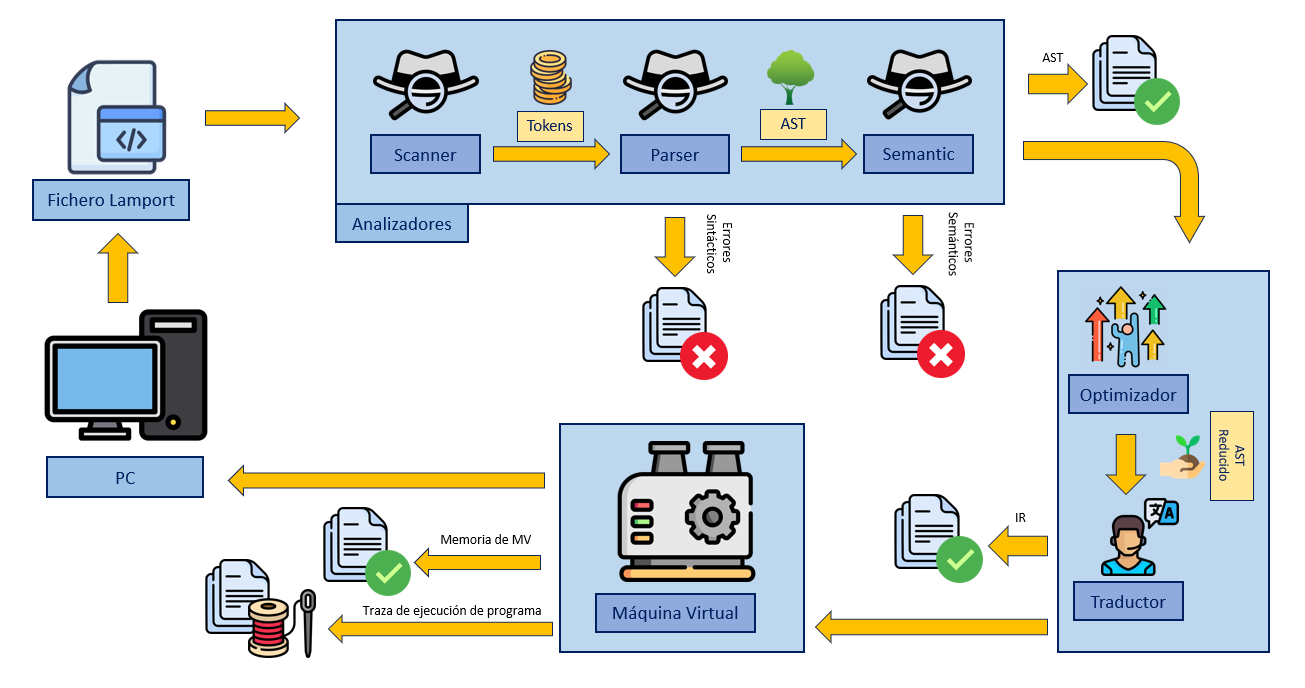
\includegraphics[width=\linewidth]{images/lmp/lmp_resume.png}
    \caption{Esquemático del intérprete de Lamport}
    \label{fig:lmpresume}
\end{figure}



\begin{itemize}
    \item \textbf{Lexer (~\ref{sec:implementacionLexer} ):} Implementa el analizador léxico con Flex. Es el primer módulo encargado de escanear el fichero, reconociendo todos los patrones y obteniendo los tokens.
    
    \item \textbf{Parser (~\ref{sec:implementacionParser} ):} Implementa el analizador sintáctico con Bison. Su función es analizar la secuencia de tokens proporcionada por el Lexer y construir una representación estructurada: un Árbol de Sintaxis Abstracta.
    
    \item \textbf{AST (~\ref{sec:implementacionAST} ):} Representa el Árbol de Sintaxis Abstracta. Es una representación gráfica estructurada del código fuente, que es creada a partir del análisis realizado por el Parser.
    
    \item \textbf{Semantic (~\ref{sec:implementacionSemantic} ):} Encargado del análisis semántico. Evalúa el AST para asegurarse de que el programa cumple con todas las reglas semánticas.
    
    \item \textbf{Error (~\ref{sec:implementacionError} ):} Gestiona y reporta errores encontrados en cualquier etapa de la interpretación, ya sea en el análisis léxico, sintáctico o semántico.
    
    \item \textbf{IR (~\ref{sec:implementacionError} ):} Representa la Representación Intermedia. Es una versión intermedia del código fuente que se utiliza para optimizaciones y para la generación final de código.
    
    \item \textbf{LVM (~\ref{sec:implementacionLVM} ):} Se refiere a la Máquina Virtual de Lamport. Este módulo ejecuta el código representado en IR, actuando como el intérprete final que produce los resultados deseados.
    
    \item \textbf{LMP\_Utils (~\ref{sec:implementacionLMPUtils} ):} Consiste en una serie de controladores que coordinan y facilitan la interacción entre los diferentes módulos del intérprete.
    
\end{itemize}

\section{Módulo de análisis léxico: ``Lexer''}\label{sec:implementacionLexer}

En esta sección se detallan los aspectos más relevantes de la implementación del analizador léxico para el lenguaje Lamport. Como se mencionó anteriormente, se ha optado por la herramienta \textbf{Flex} dado que permite implementar el diseño discutido en la sección ~\ref{subsec:tokensLamport} de manera directa y eficiente.



El módulo de análisis léxico, también conocido como ``Lexer'', actúa como un puente entre el código fuente y el analizador sintáctico. Transforma una secuencia de caracteres en una secuencia de tokens que el analizador sintáctico utiliza para construir el Árbol de Sintaxis Abstracta (AST).



Aunque el analizador léxico es una entidad independiente, su operación está intrínsecamente ligada al analizador sintáctico. Esta relación se evidencia cuando se utilizan herramientas como Flex y \textbf{Bison} en conjunto, ya que están diseñadas para trabajar de la mano. Flex se encarga de la tokenización y \textbf{Bison} del análisis sintáctico basado en esos tokens.



La implementación del analizador léxico se hizo en un fichero único, llamado \code{lexer.l}. Este archivo sigue la estructura convencional dictada por Flex y se puede desglosar en las siguientes secciones:

\begin{itemize}
    \item \textbf{Cabeceras y Funciones:} Esta sección incluye las bibliotecas necesarias y define funciones auxiliares que pueden ser requeridas durante el proceso de tokenización. Las cabeceras suelen conectar el analizador léxico con otras partes del sistema, como el analizador sintáctico.
    
    \item \textbf{Patrones de Reconocimiento:} Aquí es donde se definen las expresiones regulares que reconocen algunos de los diferentes tokens del lenguaje Lamport. Cada expresión regular está asociada a un token específico, permitiendo que el código fuente se divida en unidades significativas.
    \item \textbf{Acciones:} Para cada patrón reconocido, se puede especificar una acción. Estas acciones suelen consistir en devolver el token reconocido al analizador sintáctico, aunque también pueden incluir otras operaciones, como manejar el recuento de líneas o ignorar comentarios.
\end{itemize}

Los tokens se definen de manera explícita en una cabecera llamada \code{tokens.h}, que se deriva de la implementación del archivo de análisis sintáctico en Bison. El principal problema es que, para que Bison pueda reconocer adecuadamente los tokens, necesita estar al tanto de su existencia a través de la regla interna:
\begin{verbatim}
    %token <nombre de token>
\end{verbatim}

Esta situación destaca uno de los desafíos que surge debido a la fuerte interdependencia entre el analizador léxico y sintáctico. Sin embargo, no es un problema insuperable: Bison ofrece una opción de generación que extrae estos tokens, permitiendo su uso en otras áreas, como es el caso de la fase de análisis léxico. Mientras se trabajó en la implementación de este módulo en particular, se utilizó otra cabecera definida manualmente para lograr el mismo propósito, hasta avanzar al siguiente donde ya se genere de forma automática y detectable por en ``lexer'' y ``parser''.



Otro desafío, que se discutirá en detalle más adelante, es la gestión de cadenas de caracteres en el lenguaje C utilizando memoria dinámica. A diferencia de su sucesor, C++, en C es necesario implementar mecanismos explícitos de asignación y liberación de memoria para contener estas cadenas. El problema específico que concierne aquí surge durante el reconocimiento de secuencias de caracteres que generan los tokens \code{LITERAL} o \code{IDENT}, donde hay que llevar un registro de los punteros a estas cadenas para que puedan ser liberados adecuadamente una vez que ya no sean necesarios.

\subsection{Exposición del fichero de generación de analizador léxico: ``lexer.l''}
Se presentan algunas de las partes más interesantes dentro del fichero que sirve para generar el analizador léxico. Flex lo procesa y traduce su contenido en un archivo fuente de código C, evidentemente en el caso de que lo que contenga sea correcto.

\begin{figure}[ht]
\begin{lstlisting}[style=customflex]
%{
    //Inclusion de los tipos de Token
    #include "lexer/token.h"

    // -- Inclusion de funcion de insercion de cadena a registro de cadenas
    extern int add_string_to_register(char *str);
    // -- Inclusion de funcion de obtencion de registro de cadenas
    extern char * get_last_str_reg();
%}

/* Habilitar seguimiento de errores en la linea especifica del programa */
%option yylineno
\end{lstlisting}
\caption{Analizador Léxico: Sección de declaraciones de Flex (lexer.l)}
\label{fig:flexdeclarations}
\end{figure}

\begin{figure}[ht]
\begin{lstlisting}[style=customflex]
delim       [ \t\r\n]
nl          \n
comentario  "{"[^}]*"}"
ws          {delim}+
letra       [A-Za-z]
digito      [0-9]
entero      {digito}+
real        {digito}+\.{digito}+
id          {letra}({letra}|{digito})*
literal     \''[^'']*\''
caracter    \`.\'

\end{lstlisting}
\caption{Analizador Léxico: Sección de definición de expresiones regulares de Flex (lexer.l)}
\label{fig:flexregularExpr}
\end{figure}

\newpage

\begin{figure}[htbp]
\begin{lstlisting}[style=customflex]
"program"       {return(S_PROGRAM);}
"var"           {return(S_VAR);}
"integer"       {return(T_INTEGER);}
"boolean"       {return(T_BOOLEAN);}
"char"          {return(T_CHAR);}
"string"        {return(T_STRING);}
"real"          {return(T_REAL);}

// .... (resto de palabras reservadas) ....

{id}            {
    // -- Incluir cadena al registro de cadenas
    if(add_string_to_register(strdup(yytext)))
        yylval.ident = get_last_str_reg();
    return(IDENT);
    }
{literal}       {
    if(add_string_to_register(strdup(yytext)))
        yylval.literal_string = get_last_str_reg();
    return(LITERAL);
    }
{entero}        {
    yylval.literal_int = atoi(yytext); 
    return(L_INTEGER);
    }
{real}          {
    yylval.literal_float = atof(yytext); 
    return(L_REAL);
    }
{caracter}      {
    yylval.literal_char = yytext[1]; 
    return(L_CHAR);
    }
{comentario}    { /*IGNORAR*/ }
{ws}            { /*IGNORAR*/ }
\end{lstlisting}
\caption{Analizador Léxico: Sección de acciones de Flex (lexer.l)}
\label{fig:flexAcciones}
\end{figure}

En la última figura, se observa que, para patrones literales como las palabras reservadas del lenguaje, se retorna simplemente el token correspondiente. No obstante, para aquellos patrones que dependen de expresiones regulares, el tratamiento es más elaborado. Principalmente, se almacena su valor en una variable denominada \code{yylval}, que es una unión global utilizada por Flex para pasar información del analizador léxico al analizador sintáctico, que en este caso será el valor de un literal. En los patrones que reconocen cadenas de caracteres, primero se registran las cadenas y luego se almacenan. Por último, elementos como comentarios, saltos de línea, tabulaciones y espacios son ignorados.

Para finalizar, es fundamental destacar que el núcleo del funcionamiento del analizador léxico se encuentra en una función llamada \code{yylex()}. Esta función es generada automáticamente por Flex y se encarga de leer la entrada, reconocer patrones de texto que coinciden con las expresiones regulares definidas y, posteriormente, ejecutar las acciones asociadas a esos patrones, generalmente retornando tokens o ejecutando otras operaciones. La función \code{yylex()} actúa como el principal punto de entrada al analizador léxico y es invocada por el analizador sintáctico para obtener el siguiente token de la entrada.

\newpage

\subsection{Procesamiento de ``Hola Mundo'' utilizando el ``Lexer''}
Ya se dispone de la primera unidad operativa del intérprete, por ello, ya se puede realizar la primera interpretación del programa ``Hola Mundo'' (~\ref{fig:lamportHolaMundo} ). Habilitando un código que permita leer flujos de entrada, y pasando como argumento el fichero donde se encuentra el programa en Lamport, el resultado que muestra el analizador léxico es la siguiente lista:

\begin{figure}[h]
\begin{verbatim}
S_PROGRAM IDENT DELIM_PC
S_VAR IDENT DELIM_2P T_INTEGER DELIM_PC 

S_PROCEDURE IDENT PAR_IZDO IDENT DELIM_2P T_STRING PAR_DCHO 
B_BEGIN 
PRINT PAR_IZDO LITERAL DELIM_C IDENT DELIM_C LITERAL PAR_DCHO DELIM_PC
B_END

S_FUNCTION IDENT PAR_IZDO IDENT DELIM_2P T_INTEGER PAR_DCHO 
    DELIM_2P T_INTEGER DELIM_PC 
S_VAR IDENT DELIM_2P T_INTEGER OP_ASSIGN
    PAR_IZDO OP_MINUS L_INTEGER OP_SUM L_INTEGER PAR_DCHO OP_MULT L_INTEGER 
    OP_MINUS L_INTEGER DELIM_PC
B_BEGIN 
RETURN IDENT OP_SUM IDENT DELIM_PC 
B_END 

S_PROCESS IDENT DELIM_PC 
S_VAR IDENT DELIM_2P T_STRING OP_ASSIGN LITERAL DELIM_PC
S_VAR IDENT DELIM_2P T_INTEGER OP_ASSIGN L_INTEGER DELIM_PC
B_BEGIN 
IDENT PAR_IZDO IDENT PAR_DCHO DELIM_PC 
IDENT OP_ASSIGN IDENT PAR_IZDO IDENT PAR_DCHO DELIM_PC 
PRINT PAR_IZDO LITERAL DELIM_C IDENT PAR_DCHO DELIM_PC 
B_END
\end{verbatim}
\caption{Programa ``¡Hola Mundo!'' Lamport: Secuencia de Tokens.}
\label{fig:tokensHolaMundo}
\end{figure}

\section{Módulo de análisis sintáctico: ``Parser''}\label{sec:implementacionParser}
Una vez completada la implementación del analizador léxico, el siguiente paso es la creación del analizador sintáctico para el lenguaje Lamport. Se eligió la herramienta \textbf{Bison} por razones similares a las que motivaron la elección de Flex: su capacidad para materializar el diseño discutido en la sección \ref{subsec:sintaxisLamport} fácilmente. Como se destacó al concluir el capítulo anterior, Bison es una herramienta que genera analizadores sintácticos basados en gramáticas \code{LALR(1)}. Bison servirá precisamente para verificar que la gramática definida para Lamport cae dentro de esta categoría y, por lo tanto, puede ser procesada eficientemente.



Aquí se destacan dos problemas principales. El primero, como ya se discutió en la sección ~\ref{subsubsec:gramaticaAmbiguaLamport}, es la ambigüedad de la gramática. Hay que ser cuidadoso para garantizar que Bison reconozca correctamente qué regla aplicar. Esto puede requerir modificaciones ligeras en las reglas o la especificación de precedencias. El segundo problema radica en la gestión de errores sintácticos. Uno de los pilares fundamentales de la ingeniería informática es diseñar sistemas asumiendo que los usuarios pueden cometer errores, por lo que es crucial abordar adecuadamente estos fallos potenciales, y sobretodo, ser transparente de cara al cliente final.



El analizador sintáctico se ha definido en un fichero denominado \code{parser.y}, y que sigue la estructura también dictada por Bison:

\begin{itemize}
    \item \textbf{Cabeceras y Funciones:} Esta sección generalmente incluye cualquier archivo de cabecera requerido y define las funciones que se utilizarán a lo largo del archivo. También puede contener definiciones de tipos y otras estructuras de datos necesarias.
    
    \item \textbf{Declaración de Tokens:} Aquí se declaran todos los tokens que el analizador léxico (Lexer) proporcionará al analizador sintáctico (Parser).

    \item \textbf{Estructuras para la Construcción del AST:} Define las estructuras de datos y uniones que se utilizarán para construir el Árbol de Sintaxis Abstracta a medida que se procesan las reglas.

    \item \textbf{Asociatividad de Operaciones:} Define la precedencia de los operadores para resolver ambigüedades en las expresiones.

    \item \textbf{Especificación de Tipos de Valor Semántico:} Establece las asociaciones entre los tipos de las estructuras del AST y las reglas gramaticales. Esta sección es fundamental para las acciones semánticas, ya que determina cómo se construyen y conectan las diferentes partes del AST. Cada regla tiene un tipo específico asociado que indica qué tipo de nodo del AST se construirá o procesará cuando se aplique esa regla.

    \item \textbf{Reglas de producción:} Es el núcleo del analizador sintáctico. Define cómo las secuencias de tokens (producidas por el Lexer) se agrupan en estructuras de mayor nivel, como expresiones y sentencias.
    
    \item \textbf{Acciones semánticas:} Incrustadas dentro de las reglas de producción, estas acciones se ejecutan cuando se reconoce una regla en particular. Permiten construir el Árbol de Sintaxis Abstracta (AST), realizar comprobaciones semánticas o ejecutar código directamente.
    
    \item \textbf{Código C adicional:} Al final del archivo, se puede incluir cualquier función o estructura de datos adicional en lenguaje C que se requiera para la implementación.
\end{itemize}

\subsection{Exposición del primer fichero de generación de analizador sintáctico: ``parser.y''}
Se presentan algunas de las partes más interesantes dentro del primer fichero desarrollado que sirve para generar el analizador sintáctico. Bison lo procesa y traduce su contenido en un archivo fuente de código C, independientemente de que haya errores de reducción o desplazamiento.

\begin{figure}[h]
\begin{lstlisting}[style=customflex]
%{
    // ---------------------------------------------
    // DEFINICION DE FUNCIONES Y ESTRUCTURAS PROPIAS DE BISON

    // -- Variables y funciones a utilizar por el analizador sintactico
    extern int yylex();
    extern FILE *yyin;
    extern int yylineno;

    void yyerror(const char* s);  
%}
\end{lstlisting}
\caption{Analizador Sintáctico: Sección de declaraciones de Bison (parser.y)}
\label{fig:bisonDeclaraciones}
\end{figure}

En la figura referente al analizador sintáctico, se destaca la función \code{yylex()}, mencionada previamente en la sección anterior. Esta función es el motor del analizador léxico, y Bison la invoca internamente para obtener los tokens. Asimismo, se observa el puntero a fichero \code{yyin}. Este puntero hace referencia al descriptor del fichero que el intérprete ha abierto y está listo para ser analizado.

\newpage

\begin{figure}[h]
\begin{lstlisting}[style=customflex]
// =====================================
// DEFINICION DE TOKENS

%token S_PROGRAM 258
%token S_VAR 259
%token T_INTEGER 260
%token T_BOOLEAN 261
%token T_CHAR 262
%token T_STRING 263
%token T_REAL 264
%token T_ARRAY 265
%token T_SEMAPHORE 266
%token T_DPROCESS 267
%token S_PROCESS 268
%token S_PROCEDURE 269
%token S_FUNCTION 270
%token RETURN 271
\end{lstlisting}
\caption{Analizador Sintáctico: Sección de definición de tokens de Bison (parser.y)}
\label{fig:bisonTokens}
\end{figure}


\begin{lstlisting}[style=customflex]
program:
  // ===== CORRECTO: Programa lamport completo
  S_PROGRAM program-name list-declarations list-subprograms list-process
  ;

program-name:
    IDENT;

// -- Reglas de generacion de declaraciones del programa

list-declarations:
    declaration list-declarations
    | /* epsilon */
    ;

declaration:
    // ===== CORRECTO: Declaracion completa con asignacion
    S_VAR IDENT DELIM_2P type OP_ASSIGN expression DELIM_PC
    // ===== CORRECTO: Declaracion completa sin asignacion
    | S_VAR IDENT DELIM_2P type DELIM_PC
    ;

list-subprograms:
    subprogram list-subprograms
    | /* epsilon */
    ;

subprogram:
    subprogram-procedure
    | subprogram-function
    ;

subprogram-procedure:
    // ===== CORRECTO: Subprograma procedimiento completo (con lista de parametros)
    S_PROCEDURE subprogram-procedure-name PAR_IZDO list-parameters PAR_DCHO DELIM_PC list-declarations block-statements-begin-end
    // ===== CORRECTO: Subprograma procedimiento completo (sin lista de parametros)
    | S_PROCEDURE subprogram-procedure-name PAR_IZDO PAR_DCHO DELIM_PC list-declarations block-statements-begin-end
    ;

subprogram-procedure-name:
    IDENT
    ;

subprogram-function:
    // ===== CORRECTO: Subprograma funcion completo (con lista de parametros)
    S_FUNCTION subprogram-function-name PAR_IZDO list-parameters PAR_DCHO DELIM_2P basic-type DELIM_PC list-declarations block-statements-function
    // ===== CORRECTO: Subprograma funcion completo (sin lista de parametros)
    | S_FUNCTION subprogram-function-name PAR_IZDO PAR_DCHO DELIM_2P basic-type DELIM_PC list-declarations block-statements-function
    ;

subprogram-function-name:
    IDENT
    ;

\end{lstlisting}
\begin{figure}[h]
\caption{Analizador Sintáctico: Sección de definición de reglas sintácticas de Bison (parser.y)}
\label{fig:bisonRules}
\end{figure}

En la última figura se muestran algunas de las reglas gramaticales definidas a partir de la expresión de la gramática en notación BNF. Estas reglas corresponden a la generación de componentes específicos del lenguaje, como un programa, una declaración o un subprograma. Es notable la presencia de reglas específicas, como \code{list-declarations}'' y \code{list-subprograms}'', encargadas de generar listas de declaraciones y subprogramas, respectivamente.

Dentro de estas reglas, es crucial entender cómo se gestionan las listas. Tomando como ejemplo a ``\code{list-declarations}'', el metalenguaje BNF indica que un programa podría contener \textbf{o una o ninguna} lista de declaraciones. En caso de que haya una lista de declaraciones, deberá haber al menos una declaración dentro. Con esta estructura, Bison generará recursivamente la lista de declaraciones y continuará hasta que no se encuentren más declaraciones, en cuyo punto se reconocerá el término vacío, representado por $\epsilon$, indicando el fin de la lista.



Este primer analizador sintáctico es extremadamente sencillo, pues no se han definido acciones semánticas para ninguna regla, ni tampoco se han definido estrategias de recuperación ante errores sintácticos. El objetivo es simplemente asegurar que la gramática se puede generar sin conflictos, y una vez se haya garantizado, se irá incrementando gradualmente el refinamiento de la descripción práctica del analizador sintáctico.

\subsection{Solucionando los problemas de ambigüedad de la gramática}
Ha llegado el momento de asegurar que los conflictos derivados de la definición ambigüa de la gramática (~\ref{subsubsec:gramaticaAmbiguaLamport} ) se resuelven e implementan de la manera más eficiente para la generación del analizador sintáctico en la práctica.


\noindent
Para generar el analizador sintáctico y además asegurar que no se producen conflictos, se utilizará la siguiente orden:
\begin{verbatim}
    bison --defines=include/lexer/token.h --output=src/parser/parser.c 
        src/parser/parser.y -Wcounterexamples
\end{verbatim}

La opción más notable en este comando es \code{-Wcounterexamples}. Esta opción instruye a Bison a mostrar ejemplos concretos de entrada cuando se detectan conflictos en la gramática. Es especialmente útil ya que no sólo informa de la existencia de un conflicto, sino que también proporciona una entrada específica que lo desencadena, facilitando así la tarea de identificar y corregir el problema en la gramática.



No obstante, puesto que se está utilizando un \code{Makefile}, simplemente se aplicará la regla que incluye la orden anterior para no tener que reescribirla constantemente:
\begin{verbatim}
    $ make generate_parser
\end{verbatim}

\subsubsection{Expresiones}
En el fichero \code{parser.y} las reglas gramaticales para la generación de expresiones son las siguientes:

\newpage

\begin{lstlisting}[style=customflex]
expression:
    binary-expression
    | unary-expression
    | term
    ;

binary-expression:
    // expression + term
    expression OP_SUM expression
    // expression - term
    | expression OP_MINUS expression
    // expression * term
    | expression OP_MULT expression
    // expression / term
    | expression OP_DIV expression
    // ... (resto de operaciones binarias) ...
    ;

\end{lstlisting}
\begin{figure}[h]
\caption{Analizador Sintáctico: Sección de definición de reglas sintácticas (expresiones) de Bison (parser.y)}
\label{fig:bisonExpressionRules}
\end{figure}

\noindent
El resultado actual de ejecutar la orden especificada es el siguiente:
\begin{figure}[h]
    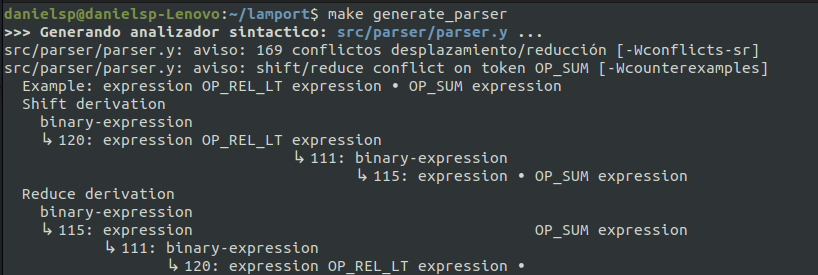
\includegraphics[width=\linewidth]{images/implementacion/parser/parser_conflicts.png}
    \caption{Conflictos de generación de parser por ambigüedad de gramática.}
    \label{fig:parser_conflictos}
\end{figure}

Se producen una inmensa cantidad de conflictos de tipo deslplazamiento/reducción (169 en total). En la captura se observa la indecisión de Bison para decantarse por una regla u otra con el ejemplo:

\begin{verbatim}
    expression OP_REL_LT expression * OP_SUM expression
\end{verbatim}

\noindent
donde se muestran dos caminos posibles para obtener la misma producción.



La solución para este problema en particular pasa por utilizar la precedencia de los operadores que ya se definió en la sección (~\ref{subsec:precOperadoresLamport} ). En Bison se puede indicar utilizando las directivas:

\begin{verbatim}
    %left <TOKEN>
    %right <TOKEN>
\end{verbatim}

\noindent
donde \code{\%left} y \code{\%right} especifican la asociatividad de las operaciones.



\noindent
Aquí se muestra cómo se aplicó la tabla de precedencia en el fichero \code{parser.y}:
\begin{lstlisting}[style=customflex]
%left OP_OR
%left OP_AND
%left OP_REL_EQ OP_REL_NEQ
%left OP_REL_LT OP_REL_LTE OP_REL_GT OP_REL_GTE
%left OP_SUM OP_MINUS
%left OP_MULT OP_DIV OP_MOD
%right OP_NOT

// ....

unary-expression:
    // not term
    OP_NOT term
    // - term
    | OP_MINUS term %prec OP_MINUS
    ;

\end{lstlisting}
\begin{figure}[h]
\caption{Analizador Sintáctico: Especificación de precedencia de operadores en Bison (parser.y)}
\label{fig:bisonPrecOperators}
\end{figure}

Los tokens que se encuentren más abajo en la lista anterior tienen \textbf{mayor prioridad}. Un caso especial es el del operador unario \code{-}, donde debe colocarse explícitamente en la regla donde se utiliza para no confundir a Bison con su homólogo binario.



Ahora el resultado es este, donde ya podemos garantizar que $G$ es una gramática \code{LALR(1)}, que es lo que queríamos demostrar al generar la gramática con Bison:
\begin{figure}[h]
    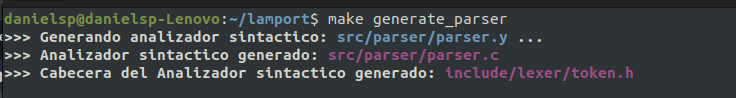
\includegraphics[width=\linewidth]{images/implementacion/parser/parser_success.png}
    \caption{Generación exitosa de la gramática de Lamport.}
    \label{fig:parser_success}
\end{figure}

\subsection{Estrategia de recuperación ante errores sintácticos}
Otro de los problemas a abordar ahora es qué hacer cuando el analizador sintáctico se encuentra con una estructura de tokens que no corresponde con ninguna de las previstas. Aquí hay dos formas posibles de implementar este mecanismo:

\begin{enumerate}
    \item Detectar un error sintáctico y detener inmediatamente el análisis mediante la directiva \code{YYABORT}. Esta acción provoca que, al identificar el primer error en el programa, este sea reconocido y gestionado adecuadamente. Acto seguido, el analizador sintáctico se detendrá, evitando el análisis del resto del fichero.
    
    \item Detectar un error sintáctico e intentar recuperarse, reanudando el análisis a partir de un token específico. En este enfoque, al encontrar un error, se gestiona y, posteriormente, se indica al analizador sintáctico un punto específico dentro de la secuencia de tokens restantes para que continúe con el análisis.
\end{enumerate}

Ambas estrategias son válidas y tienen sus méritos. Sin embargo, es esencial considerar la experiencia del usuario al decidir cuál implementar. La segunda opción, aunque es técnicamente más desafiante debido a la necesidad de identificar los puntos precisos para la recuperación, puede ofrecer una experiencia de usuario más amigable al proporcionar retroalimentación más detallada sobre múltiples errores en lugar de detenerse en el primero. Finalmente, se ha adoptado utilizar un esquema híbrido donde se implementa el primer caso para detección de patrones no esperados y el segundo para detección de errores sintácticos más precisos, como por ejemplo errores en la declaración de una variable.



Independientemente de la estrategia que se implemente, la forma de proceder es la misma, y consiste en definir reglas gramaticales explícitas que se identifiquen como un error sintáctico. A continuación, se muestra un ejemplo para el reconocimiento de errores sintácticos en una declaración de variable:

\begin{lstlisting}[style=customflex]
declaration:
    // ===== CORRECTO: Declaracion completa con asignacion
    S_VAR IDENT DELIM_2P type OP_ASSIGN expression DELIM_PC{
        // ... mas adelante tendra accian semantica ...
    }
    // ===== CORRECTO: Declaracion completa sin asignacion
    | S_VAR IDENT DELIM_2P type DELIM_PC{
        // ... mas adelante tendra accian semantica ...
    }
    // <-> ERROR: se esperaba 'var'
    | IDENT DELIM_2P type DELIM_PC{
        mark_error_syntax_declaration_expected_var($1);
        //YYABORT;
    }
    // <-> ERROR: se esperaba identificador despues de 'var'
    | S_VAR error DELIM_PC{
        mark_error_syntax_declaration_expected_identifier();
        //YYABORT;
    }
    // <-> ERROR: se esperaba ':'
    | S_VAR IDENT error DELIM_PC{
        mark_error_syntax_declaration_expected_delim2p($2);
        //YYABORT;
    };
    // <-> ERROR: se esperaba tipo de dato
    | S_VAR IDENT DELIM_2P DELIM_PC{
        mark_error_syntax_type_expected_type($2);
        //YYABORT;
    }
    // <-> ERROR: se esperaba ';'
    | S_VAR IDENT DELIM_2P type error{
        mark_error_syntax_declaration_expected_delimpc($2);
        //YYABORT;
    }
    // <-> ERROR: se esperaba operador de asignacion
    | S_VAR IDENT DELIM_2P type expression DELIM_PC{
        mark_error_syntax_declaration_expected_opassign($2);
        //YYABORT;
    }
    // <-> ERROR: se esperaba ';'
    | S_VAR IDENT DELIM_2P type OP_ASSIGN expression error{
        mark_error_syntax_declaration_expected_delimpc($2);
        //YYABORT;
    }
    ;

\end{lstlisting}
\begin{figure}[h]
\caption{Analizador Sintáctico: Sección de definición de reglas sintácticas (errores) de Bison (parser.y)}
\label{fig:bisonErrorDeclarations}
\end{figure}

En estas reglas y en todas las definidas para errores, se puede alternar fácilmente entre las estrategias mencionadas comentando o descomentando la directiva \code{YYABORT}. Además, aparece la palabra \code{error}, que es un mecanismo especial en Bison para manejar errores sintácticos. Este mecanismo permite que, en caso de errores, se salte a la parte de la gramática donde se especifica \code{error} para gestionar el fallo y tomar una acción correctiva, ya sea detener el análisis o intentar recuperarse y continuar. Es una herramienta poderosa que proporciona gran flexibilidad en el manejo de errores, permitiendo adaptar la respuesta del analizador a las necesidades específicas del contexto.



Por el momento, se definieron una serie de funciones con mensajes descriptivos en la sección de código C en Bison, que en el producto final desarrollado se movieron a un módulo encargado específicamente de la gestión de errores en el análisis y que se abordará en la sección ~\ref{sec:implementacionError}.

\subsection{Procesamiento de ``Hola Mundo'' utilizando el ``Parser''}\label{subsec:holaMundoParser}

Ahora ya se dispone de un analizador léxico y de un analizador sintáctico, lo que otorga una capacidad de cómputo considerable. Para la interpretación de programas, se utiliza la función \texttt{yyparse()}, que se encarga de iniciar el análisis sintáctico basado en las reglas gramaticales definidas. Antes de invocar a esta función, se asigna al puntero \texttt{yyin} el fichero abierto que contiene el programa, permitiendo que el analizador sintáctico lea el contenido y coordine con el analizador léxico para reconocer los tokens. Finalmente, en la regla de generación del programa completo, se introdujo un mensaje de éxito en su acción semántica. Con estas implementaciones, se procederá a la interpretación del programa ``Hola Mundo'' (~\ref{fig:lamportHolaMundo} ).



Puesto que el programa es sintácticamente correcto, el resultado de la ejecución es el siguiente:

\begin{figure}[h]
\begin{verbatim}
    ``ANÁLISIS SINTÁCTICO REALIZADO CON ÉXITO.''
\end{verbatim}
\caption{Programa ``¡Hola Mundo!'' Lamport: Resultado de análisis sintáctico (simple).}
\label{fig:parserHolaMundo}
\end{figure}

Aunque se ha avanzado significativamente con el analizador sintáctico, aún queda trabajo por hacer. Por ahora, el analizador puede determinar si un programa está bien estructurado o no, y comunicar ese resultado al usuario, pero no es suficiente porque no se realiza un tratamiento específico de cada sección del código Lamport. Por el momento, se han superado los desafíos principales relacionados con la gramática y establecido los módulos de entrada principales. El próximo paso es proporcionar al intérprete de Lamport una estructura que facilite su manipulación computacional: el AST.

\newpage

\section{Árbol de Sintaxis Abstracta (Abstract Syntax Tree,``AST'')}\label{sec:implementacionAST}
Tras completar el análisis sintáctico, surge la necesidad de representar el programa de una manera que facilite su manipulación y análisis en etapas subsecuentes. En este contexto, se introduce el Árbol de Sintaxis Abstracta (AST, por sus siglas en inglés). Un AST proporciona una representación estructurada y jerárquica de la estructura lógica del código fuente, prescindiendo de muchos detalles superficiales presentes en el texto original. En esta sección, se abordará la construcción y características del AST y se profundizará en su relevancia para el entendimiento y procesamiento del programa Lamport.

\subsection{Nodos del AST}
Dentro de la representación de un Árbol de Sintaxis Abstracta (AST), los nodos desempeñan un papel fundamental. Cada nodo refleja una construcción o elemento del lenguaje de programación, y la estructura jerárquica del árbol establece las relaciones entre estos elementos. En esta subsección, se abordarán los diferentes tipos de nodos que componen el AST, sus características y cómo contribuyen a capturar la esencia semántica del programa Lamport.



En la implementación práctica del AST, los nodos se manejan mediante punteros. Esta elección se justifica por diversas razones. Primero, usar punteros permite una gestión dinámica de memoria, lo que facilita la creación, modificación y eliminación de nodos durante el análisis sintáctico. Además, el uso de punteros posibilita la conexión directa entre nodos para formar la estructura de árbol. Esta metodología también optimiza la eficiencia en términos de memoria y acceso, dado que se evita la duplicación de datos y se permite una referencia directa a la información del nodo.


Todos los nodos citados a continuación han sido definidos mediante un \code{struct}, que es una estructura de datos en C que permite agrupar múltiples variables de diferentes tipos bajo un mismo nombre. Estos \code{structs} proporcionan una manera organizada y coherente de representar información compleja. Así, cada nodo del AST puede contener múltiples campos relevantes para su tipo específico, tales como operadores, operandos, identificadores, entre otros. 


De hecho, la estructura subyacente en la mayoría de los nodos (exceptuando el nodo raíz o padre que representa al programa completo) se basa en el concepto de \textbf{lista enlazada}, una estructura de datos muy utilizada en el ámbito de la programación. Esta estructura se emplea con el objetivo de definir secuencias de nodos de manera eficiente, indicando desde cada nodo la posición del siguiente en la lista.


\noindent
Para cada nodo además se implementaron los siguientes grupos de funciones:

\begin{itemize}
    \item \code{struct node * create_node(...)} : Función encargada de reservar memoria e inicializar un nodo en particular teniendo en cuenta los parámetros que se le han pasado a la función.
    \item \code{void free_node(struct node *)} : Función encargada de liberar la memoria reservada para el nodo pasado como parámetro.
    \item \code{void print_node(struct node *, int depth)} : Función encargada de imprimir el contenido del nodo pasado como parámetro en un flujo de salida. El entero \code{depth} especifica la profundidad del nodo en el árbol, para así poder imprimirlo en el lugar donde corresponde.
\end{itemize}



\subsubsection{Nodo de expresión ``expression''}
\noindent
Un nodo de expresión se compone de los siguientes elementos:
\begin{itemize}
    \item \code{expression_t} : tipo de expresión (\code{expression_t} es un enumerado).
    \item \code{char *} : tipo de expresión (en formato \code{string}).
    \item \code{struct expression *} : puntero a siguiente expresión. Útil para encadenar múltiples expresiones.
    \item \code{union} : engloba todas las posibles estructuras para una expresión:

    \begin{itemize}
        \item \code{struct (expression_binary_operation)} : Estructura que contiene todos los campos necesarios para el mantenimiento de una expresión binaria. Contiene:
        \begin{itemize}
            \item \code{expression_binary_t} : tipo de expresión binaria.
            \item \code{char *} : símbolo de operación.
            \item \code{int} : línea de definición de la expresión en el código.
            \item \code{struct expression *} : operando izquierdo de la expresión.
            \item \code{struct expression *} : operando derecho de la expresión.
        \end{itemize}
    \end{itemize}
    \begin{itemize}
        \item \code{struct (expression_unary_expression)} : Estructura que contiene todos los campos necesarios para el mantenimiento de una expresión unaria. Contiene:
        \begin{itemize}
            \item \code{expression_unary_t} : tipo de expresión unaria.
            \item \code{char *} : símbolo de operación.
            \item \code{int} : línea de definición de la expresión en el código.
            \item \code{struct expression *} : operando izquierdo de la expresión (el único que se necesita, pero por convención suele denominarse así).
        \end{itemize}
    \end{itemize}
    \begin{itemize}
        \item \code{struct (expression_identifier)} : Estructura que contiene todos los campos necesarios para el mantenimiento de una expresión de identificador. Contiene:
        \begin{itemize}
            \item \code{char *} nombre de identificador.
            \item \code{struct expression *} : expresión de acceso (útil para accesos a variables de tipo array).
            \item \code{int} : línea de definición de la expresión en el código.
        \end{itemize}
    \end{itemize}
    \begin{itemize}
        \item \code{struct (expression_literal)} : Estructura que contiene todos los campos necesarios para el mantenimiento de una expresión literal. Contiene:
        \begin{itemize}
            \item \code{expression_literal_t} tipo de literal.
            \item \code{union} : contiene los posibles literales: \code{int, float, char, char*, bool}.
        \end{itemize}
    \end{itemize}
    \begin{itemize}
        \item \code{struct (expression_function_inv)} : Estructura que contiene todos los campos necesarios para el mantenimiento de una llamada a función. Contiene:
        \begin{itemize}
            \item \code{char *} nombre de función.
            \item \code{struct expression *} : listado de argumentos de llamada.
            \item \code{int} : línea de definición de la expresión en el código.
        \end{itemize}
    \end{itemize}
    \begin{itemize}
        \item \code{struct expression *} : puntero a expresión que está entre paréntesis \code{()}.
    \end{itemize}
\end{itemize}

\subsubsection{Nodo de tipo de dato ``type''}
\noindent
Un nodo de tipo de dato se compone de los siguientes elementos:
\begin{itemize}
    \item \code{type_t} : tipo de dato (\code{type_t} es un enumerado).
    \item \code{char *} : tipo de dato (en formato \code{string}).
    \item \code{struct type *} : puntero a subtipo de dato, utilizado para arrays.
    \item \code{struct expression *} : línea en la que se define la declaración.
    \item \code{struct type *} : puntero a siguiente tipo, utilizado exclusivamente para definir los tipos de dato de argumentos de una llamada a función o procedimiento.
\end{itemize}

\subsubsection{Nodo de declaración de variable ``declaration''}
\noindent
Un nodo de declaración de variable se compone de los siguientes elementos:
\begin{itemize}
    \item \code{char *} : identificador del nombre de la variable.
    \item \code{struct type *} : puntero al tipo de dato de la variable.
    \item \code{struct expression *} : puntero a la expresión asignada a la variable.
    \item \code{int} : línea en la que se define la declaración.
    \item \code{struct declaration *} : puntero a la siguiente declaración.
\end{itemize}

\subsubsection{Nodo de sentencia ``statement''}
\noindent
Un nodo de sentencia se compone de los siguientes elementos:
\begin{itemize}
    \item \code{statement_t} : tipo de sentencia (\code{statement_t} es un enumerado).
    \item \code{char *} : tipo de sentencia (en formato \code{string}.
    \item \code{struct statement *} : puntero a siguiente sentencia.
    \item \code{union} : engloba todas las posibles estructuras para una sentencia:
    \begin{itemize}
        \item \code{struct (statement_assignment)} : estructura que contiene todos los campos para mantener una sentencia de asignación a variable. Contiene:
        \begin{itemize}
            \item \code{char *}: nombre de variable.
            \item \code{struct expression *}: puntero a expresión de acceso, útil cuando se trata de acceder a una posición específica de un array.
            \item \code{struct expression *}: puntero a expresión de asignación.
        \end{itemize}
    \end{itemize}
    \begin{itemize}
        \item \code{struct (statement_while)} : estructura que contiene todos los campos para mantener una sentencia de bucle while. Contiene:
        \begin{itemize}
            \item \code{struct expression *}: puntero a expresión de condición de bucle.
            \item \code{struct statement *}: puntero a bloque de sentencias de cuerpo de while.
            \item \code{int} : línea de definición de sentencia en el código.
        \end{itemize}
    \end{itemize}
    \begin{itemize}
        \item \code{struct (statement_for)} : estructura que contiene todos los campos para mantener una sentencia de bucle for. Contiene:
        \begin{itemize}
            \item \code{char *}: identificador de índice de bucle.
            \item \code{struct expression *}: puntero a expresión de inicio de bucle.
            \item \code{struct expression *}: puntero a expresión de fin de bucle.
            \item \code{struct statement *}: puntero a bloque de sentencias de cuerpo de for.
            \item \code{int} : línea de definición de sentencia en el código.
        \end{itemize}
    \end{itemize}
    \begin{itemize}
        \item \code{struct (statement_if_else)} : estructura que contiene todos los campos para mantener una sentencia de control if/else. Contiene:
        \begin{itemize}
            \item \code{struct expression *}: puntero a expresión de condición de if.
            \item \code{struct statement *}: puntero a bloque de sentencias de cuerpo de if.
            \item \code{struct statement *}: puntero a bloque de sentencias de cuerpo de else (si dispone).
            \item \code{int} : línea de definición de sentencia en el código.
        \end{itemize}
    \end{itemize}
    \begin{itemize}
        \item \code{struct (statement_procedure_inv)} : estructura que contiene todos los campos para mantener una sentencia de llamada a procedimiento. Contiene:
        \begin{itemize}
            \item \code{char *}: nombre de procedimiento.
            \item \code{struct expression *}: puntero a lista de argumentos de llamada.
            \item \code{int} : línea de definición de sentencia en el código.
        \end{itemize}
    \end{itemize}
    \begin{itemize}
        \item \code{struct (statement_fork)} : estructura que contiene todos los campos para mantener una sentencia de llamada a procedimiento. Contiene:
        \begin{itemize}
            \item \code{char *}: nombre de proceso.
            \item \code{int} : línea de definición de sentencia en el código.
        \end{itemize}
    \end{itemize}
    \begin{itemize}
        \item \code{struct (statement_join)} : estructura que contiene todos los campos para mantener una sentencia de llamada a procedimiento. Contiene:
        \begin{itemize}
            \item \code{char *}: nombre de proceso.
            \item \code{int} : línea de definición de sentencia en el código.
        \end{itemize}
    \end{itemize}
    \begin{itemize}
        \item \code{struct (statement_print)} : estructura que contiene todos los campos para mantener una sentencia de impresión. Contiene:
        \begin{itemize}
            \item \code{struct expression *}: puntero a lista de argumentos de impresión.
        \end{itemize}
    \end{itemize}
    \begin{itemize}
        \item \code{struct (statement_semaphore)} : estructura que contiene todos los campos para mantener una sentencia de operación sobre semáforo. Contiene:
        \begin{itemize}
            \item \code{char *}: identificador de semáforo.
            \item \code{int}: línea de definición de sentencia en el código.
        \end{itemize}
    \end{itemize}
    \begin{itemize}
        \item \code{struct (statement_block)} : estructura que encapsula un bloque de sentencias.
    \end{itemize}
\end{itemize}

\subsubsection{Nodo de parámetro de subprograma ``parameter''}
\noindent
Un nodo de parámetro se compone de los siguientes elementos:
\begin{itemize}
    \item \code{char *} : nombre de parámetro.
    \item \code{struct type *} : puntero a tipo de dato.
    \item \code{int *} : línea en la que se define el parámetro.
    \item \code{struct parameter *} : puntero a siguiente parámetro.
\end{itemize}

\subsubsection{Nodo de subprograma ``subprogram''}
\noindent
Un nodo de subprograma se compone de los siguientes elementos:
\begin{itemize}
    \item \code{subprogram_t}: tipo de subprograma (\code{subprogram_t} es un enumerado).
    \item \code{char *}: tipo de subprograma en formato \code{string}.
    \item \code{char *}: nombre de subprograma.
    \item \code{struct parameter *}: puntero a lista de parámetros (si posee).
    \item \code{struct declaration *}: puntero a lista de declaraciones (si posee).
    \item \code{struct statement *}: puntero  lista de sentencias.
    \item \code{struct type *}: puntero a tipo de dato de retorno (sólo funciones).
    \item \code{struct subprogram *}: puntero a siguiente subprograma.
    \item \code{int}: linea de definición de subprograma en el código.
\end{itemize}

\subsubsection{Nodo de proceso ``process''}
\noindent
Un nodo de proceso se compone de los siguientes elementos:
\begin{itemize}
    \item \code{process_t}: tipo de proceso (\code{process_t} es un enumerado).
    \item \code{char *}: tipo de proceso (en formato \code{string}).
    \item \code{char *}: nombre de proceso.
    \item \code{char *}: identificador de índice de proceso (para procesos estáticos vectorizados).
    \item \code{struct expression *}: expresión de inicio de vector de procesos.
    \item \code{struct expression *}: expresión de fin de vector de procesos.
    \item \code{struct declaration *}: lista de declaraciones (si posee).
    \item \code{struct statement *}: lista de sentencias.
    \item \code{int}: línea de definición de proceso en el código.
    \item \code{struct process *}: puntero a siguiente proceso.
\end{itemize}

\subsubsection{Nodo de programa ``program''}
\noindent
Un nodo de programa (el raíz del AST) se compone de los siguientes elementos:
\begin{itemize}
    \item \code{char *}: nombre de programa.
    \item \code{struct subprogram *}: lista de subprogramas (si posee).
    \item \code{struct declaration *}: lista de declaraciones de variables globales (si posee).
    \item \code{struct process *}: lista de procesos.
\end{itemize}

\subsection{Integración del AST en el analizador sintáctico}
Después de definir la estructura y el funcionamiento del AST, hay que usarlo. Manualmente reservar memoria e inicializar nodos no es una estrategia óptima. Es aquí donde las \textbf{acciones semánticas} en las reglas gramaticales de un analizador sintáctico generado por Bison cobran relevancia. Estas acciones semánticas tienen el objetivo de construir el AST a medida que se verifica la sintaxis de los diferentes elementos del lenguaje Lamport.


El primer paso es definir el tipo de dato que devolverán las reglas gramaticales. Para ello se utilizan las directivas:
\begin{verbatim}
    %union
    %type
\end{verbatim}


Con \code{\%union}, Bison identifica los tipos de datos disponibles para las acciones semánticas. Mientras que \code{\%type} permite especificar qué tipo de dato produce cada regla.

\newpage
\begin{figure}[h]
\caption{Analizador Sintáctico: Sección de definición de tipos de reglas en Bison (parser.y)}
\label{fig:bisonASTuniontype}
\end{figure}
\begin{lstlisting}[style=customflex]
// ================================
// ESTRUCTURAS PARA CONSTRUCCION DE AST

%union {
    struct program *prog;
    struct declaration *decl;
    struct subprogram *subprog;
    struct process *proc;
    struct statement *stmt;
    struct expression *expr;
    struct type *type;
    struct parameter *param;
    char *ident;
    char *literal_string;
    char literal_char;
    int literal_int;
    float literal_float;
    int literal_boolean;
};

// ================================
// ESPECIFICACION DE TIPOS DE VALOR SEMANTICO (PARA AST)

// ---- TIPO program
%type <prog> program

// ---- TIPO declaracion
%type <decl> declaration list-declarations

// ---- TIPO subprogram
%type <subprog> list-subprograms subprogram
%type <subprog> subprogram-procedure
%type <subprog> subprogram-function

// ---- TIPO process
%type <proc> list-process process 
%type <proc> process-def process-def-array

// ---- TIPO type
%type <type> type
%type <type> basic-or-array-type
%type <type> basic-type
%type <type> special-type

// ---- TIPO expression
%type <expr> expression 
// ....
%type <expr> expr-identifier
%type <expr> list-arguments argument
%type <expr> list-print

// ---- TIPO parameter
%type <param> list-parameters parameter

// ---- TIPO statement
%type <stmt> statement list-statements
%type <stmt> block-statements-begin-end
// ....
%type <stmt> block-statements-function
%type <stmt> block-statements-process
%type <stmt> assignment-statement 
%type <stmt> while-statement 
// ....
\end{lstlisting}



\noindent
Y ahora, en las reglas podemos definir acciones para construir el AST de forma automática, por ejemplo se muestra la generación del programa y las declaraciones de variables cuando son correctas sintácticamente:

\begin{lstlisting}[style=customflex]
program:
    // ===== CORRECTO: Programa lamport completo
    S_PROGRAM program-name list-declarations list-subprograms list-process{
        // -- Crear AST (solo si no hay errores sintacticos)
        if(!have_syntax_errors())
            AST_program = create_program($2,$3,$4,$5);
    }
    // <-> ERROR: Falta 'program' al comienzo del programa
    | program-name list-declarations list-subprograms list-process{
        mark_error_syntax_program_expected_program($1);
        // -- Abortar inmediatamente el analisis
        //YYABORT;
    }
    // <--> ERROR : Nombre de programa incorrecto
    | S_PROGRAM error list-declarations list-subprograms list-process{
        mark_error_syntax_program_expected_identifier();
        // -- Abortar inmediatamente el analisis
        //YYABORT;
    }
    ;



program-name:
    IDENT{ 
        $$ = $1;
    }
    ;

list-declarations:
    declaration list-declarations{
        if(!have_syntax_errors()){
            $$ = $1;
            $1->next = $2;
        }
        else{
            $$ = 0;
        }
    }
    | /* epsilon */{
        $$ = 0;
    }
    ;

declaration:
    // ===== CORRECTO: Declaracion completa con asignacion
    S_VAR IDENT DELIM_2P type OP_ASSIGN expression DELIM_PC{
        if(!have_syntax_errors()){
            $$ = create_declaration_variable($2, $4, $6, yylineno);
            add_declaration_to_register($$);
        }
        else{
            $$ = 0;
        }
    }
    // ===== CORRECTO: Declaracion completa sin asignacion
    | S_VAR IDENT DELIM_2P type DELIM_PC{
        if(!have_syntax_errors()){
            $$ = create_declaration_variable($2, $4, 0, yylineno);
            add_declaration_to_register($$);
        }
        else{
            $$ = 0;
        }
    }
    // .... (continua el fichero abajo).
\end{lstlisting}
\begin{figure}[h]
\caption{Analizador Sintáctico: Acciones semánticas de reglas gramaticales en Bison (parser.y)}
\label{fig:bisonActionRules}
\end{figure}

Es menester notar que aquí hay un problema a tratar que no es trivial y es parecido a uno que ya se mencionó en la implementación del analizador léxico, y es la correcta gestión de la memoria dinámica, desde la reserva hasta la liberación de los nodos, principalmente cuando el programa es incorrecto en algún punto del código Lamport, pues los nodos que son correctos se crearán y pueden no ser liberados adecuadamente en el caso de encontrarse con un error sintáctico, especialmente si se implementa la estrategia de recuperación de errores y no se decide abortar inmediatamente. 


La solución frente a esto es primero mantener un registro de los nodos que han sido creados para posteriormente liberarlos en cascada sí, y sólo sí, el AST no se ha podido generar por completo. Además, se implementa una guarda que verifica en cada regla correcta si se han producido errores sintácticos en otro punto, y en caso negativo, se genera el nodo correspondiente. En el momento en el que se detecten errores, independientemente de si la sintaxis en líneas posteriores del código es correcta o no, no se generarán más nodos.

\subsection{Procesamiento de ``Hola Mundo'' utilizando el ``Parser'' con AST}
Ahora ya se puede dar forma a nivel estructural y computacional del código Lamport, y es por ello por lo que haciendo el mismo procedimiento que en ~\ref{subsec:holaMundoParser}, se observa ahora que el procesamiento de ``Hola Mundo'' (~\ref{fig:lamportHolaMundo} ) arrojará como resultado el AST que se genere, puesto que el programa es sintácticamente correcto.

\begin{verbatim}
----> PROGRAMA LAMPORT DE NOMBRE: [HolaMundo]
================================================================

----> | DECLARACIONES DE PROGRAMA: [HolaMundo]
|-----> DECLARACION DE VARIABLE: [magico]
|       TIPO DE DATO:
|           TIPO: [integer]
|       VALOR DE INICIALIZACION:
|           <NONE>

================================================================

----> | SUBPROGRAMAS DE PROGRAMA: [HolaMundo]
|-----> NOMBRE DE SUBPROGRAMA: [SaludaUsuario] DE TIPO: [procedure]
|       TIPO DE DATO DE RETORNO:
|   ----> <NONE>
|       PARAMETROS DE SUBPROGRAMA:
|         NOMBRE DE PARAMETRO: [nombre]
|         TIPO DE DATO: [nombre]
|           TIPO: [string]

|       DECLARACIONES DE SUBPROGRAMA:
|-------> <NONE>
|       SENTENCIAS DE SUBPROGRAMA:
|-------> | SENTENCIA DE TIPO: [begin/end block]
|-----------> | SENTENCIA DE TIPO: [print statement]
|             | LISTADO DE EXPRESIONES A IMPRIMIR:
|                > EXPRESION DE TIPO: [literal string]
|                  VALOR DE LITERAL: ["Hola "]
|                > EXPRESION DE TIPO: [identifier]
|                  NOMBRE DE IDENTIFICADOR: [nombre]
|                > EXPRESION DE TIPO: [literal string]
|                  VALOR DE LITERAL: ["!"]



|-----> NOMBRE DE SUBPROGRAMA: [ObtieneNumero] DE TIPO: [function]
|       TIPO DE DATO DE RETORNO:
|         TIPO: [integer]
|       PARAMETROS DE SUBPROGRAMA:
|         NOMBRE DE PARAMETRO: [n]
|         TIPO DE DATO: [n]
|           TIPO: [integer]

|       DECLARACIONES DE SUBPROGRAMA:
|-------> DECLARACION DE VARIABLE: [constant]
|         TIPO DE DATO:
|             TIPO: [integer]
|         VALOR DE INICIALIZACION:
|            > EXPRESION DE TIPO: [binary operation]
|              SIMBOLO DE OPERACION: [-]
|              OPERANDO IZQUIERDO:
|                > EXPRESION DE TIPO: [binary operation]
|                  SIMBOLO DE OPERACION: [*]
|                  OPERANDO IZQUIERDO:
|                    > EXPRESION DE TIPO: [grouped expression]
|                      EXPRESION ENTRE ( )
|                        > EXPRESION DE TIPO: [binary operation]
|                          SIMBOLO DE OPERACION: [+]
|                          OPERANDO IZQUIERDO:
|                            > EXPRESION DE TIPO: [unary operation]
|                              SIMBOLO DE OPERACION: [-]
|                              OPERANDO IZQUIERDO:
|                                > EXPRESION DE TIPO: [literal integer]
|                                  VALOR DE LITERAL: [4]
|                          OPERANDO DERECHO:
|                            > EXPRESION DE TIPO: [literal integer]
|                              VALOR DE LITERAL: [6]
|                  OPERANDO DERECHO:
|                    > EXPRESION DE TIPO: [literal integer]
|                      VALOR DE LITERAL: [10]
|              OPERANDO DERECHO:
|                > EXPRESION DE TIPO: [literal integer]
|                  VALOR DE LITERAL: [2]

|       SENTENCIAS DE SUBPROGRAMA:
|-------> | SENTENCIA DE TIPO: [begin/end block]
|-----------> | SENTENCIA DE TIPO: [return statement]
|             | EXPRESION DE RETORNO:
|                > EXPRESION DE TIPO: [binary operation]
|                  SIMBOLO DE OPERACION: [+]
|                  OPERANDO IZQUIERDO:
|                    > EXPRESION DE TIPO: [identifier]
|                      NOMBRE DE IDENTIFICADOR: [constant]
|                  OPERANDO DERECHO:
|                    > EXPRESION DE TIPO: [identifier]
|                      NOMBRE DE IDENTIFICADOR: [n]



================================================================

----> | PROCESOS DEL PROGRAMA: [HolaMundo]
|-----> | NOMBRE DE PROCESO: [Main] DE TIPO: [individual process]

|-----> | DECLARACIONES DE PROCESO:
|---------> DECLARACION DE VARIABLE: [usuario]
|           TIPO DE DATO:
|               TIPO: [string]
|           VALOR DE INICIALIZACION:
|              > EXPRESION DE TIPO: [literal string]
|                VALOR DE LITERAL: ["Daniel"]

|---------> DECLARACION DE VARIABLE: [numero]
|           TIPO DE DATO:
|               TIPO: [integer]
|           VALOR DE INICIALIZACION:
|              > EXPRESION DE TIPO: [literal integer]
|                VALOR DE LITERAL: [23]


|-----> | SENTENCIAS DE PROCESO:
|---------> | SENTENCIA DE TIPO: [begin/end block]
|-------------> | SENTENCIA DE TIPO: [procedure invocation]
|               | INVOCACION DE PROCEDIMIENTO DE NOMBRE: [SaludaUsuario]
|               | LISTADO DE ARGUMENTOS DE INVOCACION DEL PROCEDIMIENTO:
|                  > EXPRESION DE TIPO: [identifier]
|                    NOMBRE DE IDENTIFICADOR: [usuario]

|-------------> | SENTENCIA DE TIPO: [assignment]
|               | ASIGNACION A VARIABLE: [magico]
|               | EXPRESION ASIGNADA A VARIABLE:
|                  > EXPRESION DE TIPO: [function invocation]
|                    INVOCACION DE FUNCION DE NOMBRE: [ObtieneNumero]
|                    LISTADO DE ARGUMENTOS DE INVOCACION DE FUNCION:
|                      > EXPRESION DE TIPO: [identifier]
|                        NOMBRE DE IDENTIFICADOR: [numero]

|-------------> | SENTENCIA DE TIPO: [print statement]
|               | LISTADO DE EXPRESIONES A IMPRIMIR:
|                  > EXPRESION DE TIPO: [literal string]
|                    VALOR DE LITERAL: ["El numero magico vale: "]
|                  > EXPRESION DE TIPO: [identifier]
|                    NOMBRE DE IDENTIFICADOR: [magico]
\end{verbatim}
\begin{figure}[hbtp]
\caption{Programa ``¡Hola Mundo!'' Lamport: Resultado de análisis sintáctico (AST).}
\label{fig:ASTHolaMundo}
\end{figure}

\newpage

\section{Módulo de análisis semántico: ``Semantic''}\label{sec:implementacionSemantic}
Tras la construcción y análisis del Árbol de Sintaxis Abstracta (AST) mediante el analizador sintáctico, emerge la necesidad de comprender más profundamente el significado de las construcciones presentes en el lenguaje. En esta sección, se introduce el módulo de análisis semántico, que tiene como principal objetivo validar que el programa cumple no solo con las reglas gramaticales del lenguaje Lamport, sino también con las reglas de contexto y las relaciones semánticas que determinan la coherencia y correctitud del código. A través de esta fase, se asegura que el código fuente tiene un sentido lógico y se prepara para las etapas subsiguientes del proceso de interpretación.

\subsection{La tabla de Símbolos}
Dentro del proceso de análisis semántico, es necesario mantener un registro organizado de todas las entidades definidas y utilizadas en el código fuente, desde variables y constantes hasta funciones y procedimientos. Este registro es conocido como la \textbf{tabla de símbolos}. La tabla de símbolos no solo almacena información sobre la declaración de estas entidades, sino también detalles relevantes como su tipo, alcance, y en algunos casos, valores iniciales o información de memoria. Su principal función es facilitar la detección de errores que mencionaremos más adelante.

\subsubsection{Ámbito de variable (scope)}
Uno de los conceptos más fundamentales en la programación y en el análisis semántico es el \textbf{ámbito de una variable}, también conocido como su ``scope''. El ámbito determina en qué partes del código una variable es accesible y dónde puede ser utilizada. Así, dependiendo de dónde se declare una variable, su visibilidad y accesibilidad pueden estar restringidas a un bloque específico de código, a una función o procedimiento, o incluso a todo el programa. Esta característica permite evitar conflictos de nombres y proporciona un grado de encapsulación, esencial para la modularidad y la estructuración de programas complejos.



\noindent
En primer lugar, se definen dos fundamentales ámbitos para una variable:
\begin{itemize}
    \item \textbf{Variable global}: Una variable global es reconocida y accesible por cualquier componente del código Lamport. Se define al principio del programa.
    \item \textbf{Variable local}: Una variable local sólo es reconocida y accesible desde el elemento donde se declaró, que en este caso puede corresponder a un subprograma específico o un proceso.
\end{itemize}

Para realizar un adecuado tratamiento de los ``scopes'', es lógico pensar que la tabla de símbolos no debe contener simplemente símbolos, sino además debe registrarse en qué ambito está definida una determinada variable. Lo más eficiente para hacer esto es considerar una \textbf{tabla Hash} con un tamaño fijo. 


Una tabla hash, también conocida como mapa hash o diccionario, es una estructura de datos que permite asociar pares de clave-valor. Utiliza una función hash para computar un índice en un array de cubetas o ranuras, desde el que se puede localizar el valor deseado. Esta estructura es especialmente útil cuando se desea un acceso rápido a los datos, ya que la función hash tiene como objetivo distribuir las claves de manera uniforme a lo largo de la tabla, permitiendo así una búsqueda, inserción y eliminación de elementos con un tiempo promedio constante. En el contexto de la gestión de ámbitos en la tabla de símbolos, las claves son un número identificador obtenido de aplicar una función hash determinada al nombre del símbolo, siendo el valor que almacena el propio símbolo.

\subsubsection{Implementación de la tabla con una pila de tablas hash}
Para implementar la tabla de forma adecuada teniendo en cuenta los diferentes ``scopes'' posibles en función del número de declaraciones, subprogramas o procesos, la mejor estructura de datos posible es una \textbf{pila de tablas hash}.

Una \textbf{pila de tablas hash} no es más que una colección de tablas hash estructuradas en forma de pila. Cada vez que se entra en un nuevo ámbito (por ejemplo, al ingresar a un subprograma o proceso), se introduce una nueva tabla hash vacía en la cima de la pila. Los símbolos definidos dentro de este ámbito se añaden a esta tabla. Cuando se sale del ámbito, simplemente se retira la tabla hash de la cima de la pila, descartando de esta forma todos los símbolos asociados a ese ámbito en particular.

La ventaja de esta aproximación es que facilita la resolución de referencias a símbolos. Al buscar un símbolo, se empieza por la tabla hash en la cima de la pila (el ámbito actual) y se va descendiendo a través de las tablas de ámbitos exteriores hasta encontrar el símbolo o llegar al fondo de la pila. Esta estructura asegura que siempre se resuelve al símbolo más cercano en términos de ámbito, que es el comportamiento deseado en la mayoría de los lenguajes de programación.

Además, la naturaleza efímera de los ámbitos internos (que se crean y descartan con frecuencia) es manejada de manera natural por la pila. Una vez que se sale de un ámbito, su correspondiente tabla hash se descarta, liberando la memoria y garantizando que los símbolos de ese ámbito no puedan ser referenciados erróneamente en un contexto donde no tienen validez.

{
\centering

\includegraphics[width=200px, height=200px]{images/implementacion/semantic/scope_stack.png}\\
}
Se puede imaginar la tabla de símbolos como una pila de diccionarios donde cada uno contiene símbolos de un único y particular ámbito. Primero se busca en el primer libro que aparece, y si no se encuentra, se va descendiendo poco a poco hasta el final.

\subsection{Resolución de nombres}
La primera fase que debe abordar el analizador semántico es lo que se denomina como \textbf{resolución de nombres}. Esto se refiere a determinar a qué entidad de un programa se refiere un nombre en particular en un contexto dado. Aunque puede parecer trivial, la correcta resolución de nombres es fundamental para garantizar la coherencia y la correcta ejecución del código. 



Para llevar a cabo esta tarea, se deben enfrentar varios desafíos. En primer lugar, es necesario identificar y gestionar los distintos ámbitos o ``scopes'' en los que un nombre puede estar definido. Como se ha visto en secciones anteriores, la estructura de una pila de tablas hash es útil en este aspecto. Cada ámbito tiene su propia tabla hash, y al buscar un nombre, se consulta primero la tabla del ámbito actual, avanzando hacia ámbitos más externos si es necesario.


El esquema general del algoritmo de resolución de nombres es el siguiente, aplicándolo desde el nodo raíz del AST (\code{program}):
\begin{enumerate}
    \item Al inicio del análisis:
    \begin{enumerate}
        \item Insertar el ``scope'' global en la pila.
    \end{enumerate}
    \item Si se trata de un bloque de declaraciones:
    \begin{enumerate}
        \item Comprobar si ya existe un símbolo en la tabla de símbolos para la variable actual a analizar.
        \begin{itemize}
            \item En caso afirmativo, se trata de un \textbf{error de redefinición de variable}.
            \item En otro caso, se crea el símbolo y se inserta en el ``scope''.
        \end{itemize}
        \item Continuar con el resto de variables hasta que no queden.
    \end{enumerate}
    \item Si se trata de un bloque de sentencias/expresiones:
    \begin{itemize}
        \item Aplicar resolución de nombres a cada sentencia o expresión hasta que no queden, buscando en todos los scopes las posibles referencias a símbolos que puedan haber.
        \begin{itemize}
            \item Si no se encuentra una referencia a un símbolo dentro de unas estructuras, se trata de un \textbf{error de uso de símbolo no declarado}, ya sea de variable, subprograma o proceso.
        \end{itemize}
    \end{itemize}
    \item Si se trata de un bloque de subprogramas:
    \begin{enumerate}
        \item Comprobar para el scope global y para el subprograma actual a analizar si ya existe un símbolo en la tabla de símbolos asociado a su identificador.
        \begin{itemize}
            \item En caso afirmativo, se tata de un \textbf{error de redefinición de subprograma}.
            \item En otro caso, se crea el símbolo y se inserta en el ``scope''.
        \end{itemize}
        \item Insertar un nuevo ``scope'' en la pila.
        \item Aplicar resolución de nombres a las declaraciones del subprograma.
        \item Aplicar resolución de nombres a las sentencias del subprograma.
        \item Retirar el ``scope'' actual de la pila.

        \item Continuar con el resto de subprogramas hasta que no queden.
    \end{enumerate}
    \item Si se trata de un bloque de procesos:
    \begin{enumerate}
        \item Comprobar para el scope global y para el proceso actual a analizar si ya existe un símbolo en la tabla de símbolos asociado a su identificador.
        \begin{itemize}
            \item En caso afirmativo, se tata de un \textbf{error de redefinición de proceso}.
            \item En otro caso, se crea el símbolo y se inserta en el ``scope''.
        \end{itemize}
        \item Insertar un nuevo ``scope'' en la pila.
        \item Aplicar resolución de nombres a las declaraciones del proceso.
        \item Aplicar resolución de nombres a las sentencias del proceso.
        \item Retirar el ``scope'' actual de la pila.

        \item Continuar con el resto de procesos hasta que no queden.
    \end{enumerate}
\end{enumerate}

\subsection{Comprobación de tipos}
Esta fase garantiza que las operaciones y asignaciones realizadas en el código fuente son coherentes desde el punto de vista de los tipos de datos involucrados. Así, se evita que, por ejemplo, se intente sumar un número entero con una cadena de texto o que se asigne un valor de tipo real a una variable que espera un valor booleano.



La comprobación de tipos no solo proporciona seguridad en la ejecución al detectar errores potenciales en una etapa temprana del proceso de compilación, sino que también contribuye a la claridad y robustez del código. Aquí es donde entra en juego la descripción semántica que se hizo del lenguaje Lamport en ~\ref{subsec:semanticaLamport}, porque se aplicará directamente en este apartado del analizador semántico.



Con respecto a la comprobación de tipos \textit{per se} no hay ninguna dificultad técnica. La forma de proceder es prácticamente idéntica a la del algoritmo de resolución de nombres, recorriendo el AST comprobando todos los nodos importantes:

\begin{enumerate}
    \item Si se trata de una expresión:
    \begin{itemize}
        \item Comprobar que se verifican todas las restricciones semánticas definidas en ~\ref{subsubsec:restriccionesSemanticas} y que refieren a expresiones.
        \item En caso contrario, se produce un \textbf{error de comprobación de tipos entre operandos de expresión}.
        \item En el caso de una expresión de llamada a función, se debe comprobar que el tipo de los argumentos pasados coincide con el de los parámetros que se definieron para la función, en el mismo orden en el que aparecen éstos.
    \end{itemize}
    \item Si se trata de una declaración de variable y además tiene un valor de inicio:
    \begin{itemize}
        \item Comprobar que el tipo de dato de la variable coincide con la evaluación del tipo de dato que emite la expresión de inicialización.
        \item En caso contrario, se produce un \textbf{error de asignación de tipos}.
    \end{itemize}
    \item Si se trata de un subprograma:
    \begin{itemize}
        \item Comprobar que se verifican todas las restricciones semánticas definidas en ~\ref{subsubsec:restriccionesSemanticas} y que refieren a subprogramas.
        \item En caso contrario, se produce un \textbf{error de comprobación de tipos}.
    \end{itemize}
    \item Si se trata de una sentencia:
    \begin{itemize}
        \item Si se está realizando una sentencia de asignación, mismo tratamiento que en el caso de inicialización de variables.
        \item En el caso de bucles while y estructuras if/else, la expresión de condición debe emitir el tipo \code{boolean}.
        \item En el caso de bucles for, las expresiones de inicio y fin deben emitir el tipo \code{integer}.
        \item En el caso de una llamada a procedimiento, se debe comprobar que el tipo de los argumentos pasados coincide con el de los parámetros que se definieron para el procedimiento, en el mismo orden en el que aparecen éstos.
        \item Todo lo anterior que no se verifique será un \textbf{error de comprobación de tipos ó de asignación}.
    \end{itemize}
\end{enumerate}

\subsection{Procesamiento de ``Hola Mundo'' utilizando el ``Semantic''}
Ahora ya se dispone de todos los analizadores posibles para un lenguaje de programación cualquiera, en particular para el lenguaje Lamport. Adaptando el código del intérprete ahora cuando se supere la fase del analizador sintáctico, se recorrerá el AST generado analizando semánticamente el programa. Primero se aplica resolución de nombres y posteriormente la comprobación de tipos. Si el procesamiento de ``Hola Mundo'' (~\ref{fig:lamportHolaMundo} ) se ha superado, se verá un mensaje de éxito en pantalla. En caso contrario se mostrarán todos los errores semánticos emitidos:



\noindent
Puesto que el programa es semánticamente correcto, el mensaje que se muestra es:
\begin{verbatim}
    ``RESOLUCIÓN DE NOMBRES Y COMPROBACIÓN DE TIPOS 
        REALIZADOS CON ÉXITO.''
\end{verbatim}

\section{Módulo de gestión de errores: ``Error''}\label{sec:implementacionError}
En los módulos de análisis sintáctico (~\ref{sec:implementacionParser} ) y análisis semántico (~\ref{sec:implementacionSemantic} ) se ha comentado la importancia que tiene realizar una gestión adecuada de los errores, y sobretodo, ser transparente en la manera de tratarlos y mostrarlos al usuario del intérprete.


Es por ello que se decidió diseñar un módulo que se encargue específicamente de la gestión de sendos errores, definiendo para ello una estructura común denominada \code{error} que contiene los siguientes campos:

\begin{itemize}
    \item \code{error_type_t}: Especifica el tipo de error (sintáctico o semántico).
    \item \code{int}: Indica la línea en el fichero del código Lamport donde se produjo el error.
    \item \code{msg}: Mensaje de error.
    \item \code{struct error *}: puntero a siguiente error, útil para mostrar múltiples errores.
    \item \code{union}: engloba información adicional sobre los diferentes tipos de error.
    \begin{itemize}
        \item \code{struct (error_syntax)}: contiene información adicional acerca de un error sintáctico:
        \begin{itemize}
            \item \code{error_syntax_t}: tipo de error sintáctico.
            \item \code{char *}: identificador de función, procedimiento, declaración o proceso donde se produjo el error sintáctico.
        \end{itemize}
    \end{itemize}
    \begin{itemize}
        \item \code{struct (error_semantic)}: contiene información adicional acerca de un error semántico:
        \begin{itemize}
            \item \code{error_semantic_t}: tipo de error semántico.
            \item \code{int}: (def\_line) sirve para errores del tipo \textbf{redefinición}, pues se indica en qué parte del fichero de código se definió un determinado símbolo.
            \item \code{int}: (which) también sirve para errores de tipo \textbf{redefinición} cuando se trata de parámetros de subprograma, indicando la posición del parámetro.
            \item \code{char *}: identificador del símbolo que produjo el error semántico.
        \end{itemize}
    \end{itemize}
\end{itemize}


El manejador de errores se integra tanto en el analizador sintáctico como en el semántico. En el primer módulo, las funciones encargadas de marcar los errores se llaman dentro de las reglas sintácticas que son tratadas como errores, mientras que en el segundo módulo simplemente se van realizando llamadas conforme se detecten aplicando los algoritmos descritos anteriormente.


Para finalizar, aquí se muestra el orden en el que aparecen los errores, dependiendo del éxito o no de la superación de las fases de análisis:

\begin{enumerate}
    \item Si no supera el análisis sintáctico, imprimir listado de errores sintácticos producidos.
    \item En caso contrario, si no supera el procedimiento de resolución de nombres, imprimir los errores semánticos producidos.
    \item En caso contrario, si no supera el procedimiento de comprobación de tipos, imprimir los errores semánticos producidos.
\end{enumerate}

\section{Módulo de gestión de Representación Intermedia: ``IR''}\label{sec:implementacionIR}
La transformación y optimización del código fuente en lenguajes de programación suele requerir una etapa intermedia antes de llegar a la fase de generación del código máquina o bytecode, o sencillamente interpretación en el caso particular de este lenguaje. Esta etapa se materializa a través de la Representación Intermedia (IR, por sus siglas en inglés). El módulo ``IR'' se encarga precisamente de gestionar esta representación, que actúa como un puente entre el análisis semántico del código fuente y su traducción final.


Esta representación simplifica y estandariza las operaciones posteriores en el proceso de interpretación, permitiendo optimizaciones y transformaciones sobre una estructura común y coherente. La IR puede adoptar diferentes formas, desde árboles hasta grafos o secuencias de instrucciones, y su diseño adecuado es crucial para el rendimiento y eficacia del intérprete.


A lo largo de esta sección, se describirá la estructura y funcionalidades del módulo ``IR'', así como la importancia y las ventajas de utilizar una Representación Intermedia en el proceso de interpretación.

\subsection{Elección de Representación Intermedia}
Al igual que se realizó un estudio meticuloso para definir el lenguaje Lamport, ahora hay que hacer lo mismo con lenguaje de representación intermedia. Para este proyecto, se optó por una representación intermedia basada en registros, lo cual brinda una organización más clara y directa del flujo de datos y operaciones. Esta elección deriva naturalmente en el uso de \textbf{instrucciones} que detallan cómo se manejan y procesan esos registros. Este enfoque no solo simplifica la representación, sino que además facilita la posterior simulación del funcionamiento de un sistema concurrente en la máquina virtual implementada.


\noindent
Una instrucción consta de los siguientes elementos:

\begin{itemize}
    \item \textbf{Código de instrucción}: Es un identificador que sirve para indicar a la posterior máquina virtual el tipo de instrucción que va a ejecutar.
    \item \textbf{Operando de destino}: Identificador que representa el lugar donde el resultado de la acción que realizará la entidad que ejecute la instrucción se almacenará.
    \item \textbf{Operando 1}: Identificador que representa al dato del primer operando de la instrucción.
    \item \textbf{Operando 2}: Identificador que representa al dato del segundo operando de la instrucción.
\end{itemize}

Los operandos son elementos que determinan las fuentes de datos o valores con los que se realizará la operación indicada por el código de instrucción. Estos pueden ser constantes, registros, direcciones de memoria, entre otros. La cantidad y el tipo de operandos pueden variar según la instrucción, y su correcta interpretación es crucial para el adecuado funcionamiento de la máquina virtual y la ejecución del programa. En esta representación intermedia, hay estos tipos de operandos:

\begin{itemize}
    \item \textbf{Identificación de un registro}: El operando apunta a un registro de la máquina virtual.
    \item \textbf{Identificación de un literal}: El operando apunta a un literal.
    \item \textbf{Identificación de una variable}: El operando apunta a una variable.
    \item \textbf{Identificación de una variable array}: El operando apunta a un elemento en concreto de una variable array.
    \item \textbf{Identificación de una etiqueta}: El operando apunta a la dirección de una etiqueta.
    \item \textbf{Identificación de un proceso/hebra}: El operando contiene el identificador del proceso.
    \item \textbf{Identificación de un salto directo}: El operando contiene la dirección de la siguiente instrucción a la que el proceso debe saltar. Tiene un comportamiento similar al de una etiqueta, pero sin especificar un nombre para la misma.
\end{itemize}

Sobre el último tipo de operando mostrado en la enumeración anterior, un aspecto clave en la representación intermedia y su ejecución en la máquina virtual son las \textbf{etiquetas}. En este contexto, una etiqueta no es más que un marcador o referencia que identifica una posición específica dentro del conjunto de instrucciones. Estas etiquetas son imprescindibles para instrucciones de control de flujo, como saltos condicionales o incondicionales, bucles, entre otros.



Por ejemplo, al encontrarse con una instrucción de salto que tiene una etiqueta como operando, la máquina virtual sabe exactamente a qué punto de la lista de instrucciones debe ``saltar'' y continuar con la ejecución desde allí. Las etiquetas, por lo tanto, ofrecen una forma de organizar y controlar el flujo de la ejecución de instrucciones en la representación intermedia, permitiendo la implementación de estructuras lógicas y de control complejas. No obstante, se tratará este aspecto más adelante.


Finalmente, en este lenguaje de representación intermedia hay un total de \textbf{5 tipos de instrucciones diferentes}:

\begin{itemize}
    \item \textbf{1 destino y 2 operandos}: la instrucción a ejecutar necesita de dos operandos y el resultado se almacenará en un destino.
    \item \textbf{1 destino y 1 operando}: la instrucción a ejecutar necesita un operando y el resultado se almacena en un destino.
    \item \textbf{1 operando}: la instrucción a ejecutar necesita un operando, y no hay necesidad de almacenar el resultado de la acción.
    \item \textbf{0 destinos y 2 operandos}: la instrucción dispone de dos operandos pero no se almacena el resultado de la ejecución en un destino.
    \item \textbf{0 destinos y 0 operandos}: la instrucción sólo dispone de su código de instrucción, suficiente para su ejecución.
\end{itemize}

\subsection{Repertorio de instrucciones de IR}
A continuación se realiza un estudio detallado del repertorio de instrucciones definido para la representación intermedia del lenguaje Lamport.

\renewcommand{\arraystretch}{1.5}
\begin{longtable}{|c|c|c|c|c|}
\caption{Repertorio de instrucciones de Representación Intermedia.} \label{tab:instruccionesIR} \\
\hline
\textbf{CÓDIGO} & \textbf{DETALLES} & \textbf{OP. DEST.} & \textbf{OP. 1} & \textbf{OP. 2} \\
\hline
\endfirsthead

\multicolumn{5}{c}%
{{\bfseries \tablename\ \thetable{} -- continuación de la página anterior}} \\
\hline
\textbf{CÓDIGO} & \textbf{DETALLES} & \textbf{OP. DEST.} & \textbf{OP. 1} & \textbf{OP. 2} \\
\hline
\endhead

\hline \multicolumn{5}{|r|}{{Continúa en la siguiente página}} \\
\hline
\endfoot

\hline
\endlastfoot
\code{IR_LABEL} & ~\ref{subsubsec:IR_LABEL}  & NO & SÍ & NO \\
\hline
\code{IR_OP_LOAD} & ~\ref{subsubsec:IR_OP_LOAD}  & SÍ & SÍ & NO \\
\hline
\code{IR_OP_STORE} & ~\ref{subsubsec:IR_OP_STORE} & SÍ & SÍ & NO \\
\hline
\code{IR_OP_ADD_[I|F]} \footnote{Aquí y en el resto de instrucciones aritméticas, ``I'' denota que la instrucción involucra a operandos de tipo \textbf{entero}, mientras que ``F'' hace lo mismo con operandos de tipo \textbf{real}.} & ~\ref{subsubsec:IR_OP_ADD} & SÍ & SÍ & SÍ \\
\hline
\code{IR_OP_SUB_[I|F]} & ~\ref{subsubsec:IR_OP_SUB} & SÍ & SÍ & SÍ \\
\hline
\code{IR_OP_MULT_[I|F]} & ~\ref{subsubsec:IR_OP_MULT} & SÍ & SÍ & SÍ \\
\hline
\code{IR_OP_DIV_[I|F]} & ~\ref{subsubsec:IR_OP_DIV} & SÍ & SÍ & SÍ \\
\hline
\code{IR_OP_MOD_I} & ~\ref{subsubsec:IR_OP_MOD} & SÍ & SÍ & SÍ \\
\hline
\code{IR_OP_NEG_[I|F]} & ~\ref{subsubsec:IR_OP_NEG} & SÍ & SÍ & SÍ \\
\hline
\code{IR_OP_AND} & ~\ref{subsubsec:IR_OP_AND} & SÍ & SÍ & SÍ \\
\hline
\code{IR_OP_OR} & ~\ref{subsubsec:IR_OP_OR} & SÍ & SÍ & SÍ \\
\hline
\code{IR_OP_NOT} & ~\ref{subsubsec:IR_OP_NOT} & SÍ & SÍ & SÍ \\
\hline
\code{IR_OP_CMP_LT} & ~\ref{subsubsec:IR_OP_CMP_LT} & SÍ & SÍ & SÍ \\
\hline
\code{IR_OP_CMP_LTE} & ~\ref{subsubsec:IR_OP_CMP_LTE} & SÍ & SÍ & SÍ \\
\hline
\code{IR_OP_CMP_GT} & ~\ref{subsubsec:IR_OP_CMP_GT} & SÍ & SÍ & SÍ \\
\hline
\code{IR_OP_CMP_GTE} & ~\ref{subsubsec:IR_OP_CMP_GTE} & SÍ & SÍ & SÍ \\
\hline
\code{IR_OP_CMP_EQ} & ~\ref{subsubsec:IR_OP_CMP_EQ} & SÍ & SÍ & SÍ \\
\hline
\code{IR_OP_CMP_NEQ} & ~\ref{subsubsec:IR_OP_CMP_NEQ} & SÍ & SÍ & SÍ \\
\hline
\code{IR_OP_JMP} & ~\ref{subsubsec:IR_OP_JMP} & NO & SÍ & NO \\
\hline
\code{IR_OP_JMP_TRUE} & ~\ref{subsubsec:IR_OP_JMP_TRUE} & NO & SÍ & NO \\
\hline
\code{IR_OP_JMP_FALSE} & ~\ref{subsubsec:IR_OP_JMP_FALSE} & NO & SÍ & NO \\
\hline
\code{IR_OP_CALL} & ~\ref{subsubsec:IR_OP_CALL} & NO & SÍ & NO \\
\hline
\code{IR_OP_RET} & ~\ref{subsubsec:IR_OP_RET} & NO & SÍ & NO \\
\hline
\code{IR_OP_PUSH} & ~\ref{subsubsec:IR_OP_PUSH} & NO & SÍ & NO \\
\hline
\code{IR_OP_POP} & ~\ref{subsubsec:IR_OP_POP} & NO & SÍ & NO \\
\hline
\code{IR_OP_PRINT} & ~\ref{subsubsec:IR_OP_PRINT} & NO & SÍ & NO \\
\hline
\code{IR_END_PRINT} & ~\ref{subsubsec:IR_END_PRINT} & NO & NO & NO \\
\hline
\code{IR_START_PROGRAM} & ~\ref{subsubsec:IR_START_PROGRAM} & NO & NO & NO \\
\hline
\code{IR_END_PROGRAM} & ~\ref{subsubsec:IR_END_PROGRAM} & NO & NO & NO \\
\hline
\code{IR_START_PROCESS} & ~\ref{subsubsec:IR_START_PROCESS} & NO & SÍ & NO \\
\hline
\code{IR_START_DPROCESS} & ~\ref{subsubsec:IR_START_DPROCESS} & SÍ & SÍ & SÍ \\
\hline
\code{IR_END_PROCESS} & ~\ref{subsubsec:IR_END_PROCESS} & NO & SÍ & NO \\
\hline
\code{IR_WAIT_PROCESS} & ~\ref{subsubsec:IR_WAIT_PROCESS} & NO & SÍ & NO \\
\hline
\code{IR_SLEEP_PROCESS} & ~\ref{subsubsec:IR_SLEEP_PROCESS} & NO & SÍ & NO \\
\hline
\code{IR_OP_ATOMIC_BEGIN} & ~\ref{subsubsec:IR_OP_ATOMIC_BEGIN} & NO & NO & NO \\
\hline
\code{IR_OP_ATOMIC_END} & ~\ref{subsubsec:IR_OP_ATOMIC_END} & NO & NO & NO \\
\hline
\code{IR_OP_SEM_WAIT} & ~\ref{subsubsec:IR_OP_SEM_WAIT} & NO & SÍ & NO \\
\hline
\code{IR_OP_SEM_SIGNAL} & ~\ref{subsubsec:IR_OP_SEM_SIGNAL} & NO & SÍ & NO \\
\hline
\code{IR_START_INIT_GLOBAL_VAR} & ~\ref{subsubsec:IR_START_INIT_GLOBAL_VAR} & NO & NO & NO \\
\hline
\code{IR_END_GLOBAL_VAR} & ~\ref{subsubsec:IR_END_INIT_GLOBAL_VAR} & NO & NO & NO \\
\end{longtable}
\renewcommand{\arraystretch}{1.0}

\subsubsection{Instrucción IR\_LABEL}\label{subsubsec:IR_LABEL}
\noindent
\textbf{Funcionalidad:} Representa a una etiqueta

\noindent
\textbf{Argumentos:} La estructura de la instrucción es la siguiente:
\begin{verbatim}
IR_LABEL <operando1>
\end{verbatim}
\begin{itemize}
    \item <\code{operando1}>: Etiqueta que delimita una sección.
\end{itemize}

\noindent
\textbf{Ejecución de la instrucción:}


\noindent
Se incrementa el contador de programa y se sigue el flujo de ejecución normal.


\noindent
\textbf{Ejemplo de uso:}
\begin{verbatim}
IR_LABEL etq1
\end{verbatim}

\subsubsection{Instrucción IR\_OP\_LOAD}\label{subsubsec:IR_OP_LOAD}
\noindent
\textbf{Funcionalidad:} Carga un valor de una variable en un registro.

\noindent
\textbf{Argumentos:} La estructura de la instrucción es la siguiente:
\begin{verbatim}
IR_OP_LOAD <registro_destino> <operando1>
\end{verbatim}
\begin{itemize}
    \item <\code{registro_destino}>: registro donde se almacenará el valor de la variable.
    \item <\code{operando1}>: Es una \code{variable}. Su valor se cargará en el registro de destino.
\end{itemize}

\noindent
\textbf{Ejecución de la instrucción:}
\noindent
Se realizan los siguientes pasos para la ejecución de la instrucción:

\begin{enumerate}
    \item El valor de <\code{operando1}> se carga en <\code{registro_destino}>.
\end{enumerate}

\noindent
\textbf{Ejemplo de uso:}
\noindent
Suponiendo que \code{y} es una variable:

\begin{verbatim}
IR_OP_LOAD R1, y
\end{verbatim}

\noindent
\textbf{Comentarios adicionales:}

La representación a nivel de código de esta instrucción realmente contendrá en el operando un entero apuntador a una tabla de variables indexada donde se encuentra el nombre de dicha variable \texttt{y}.

\subsubsection{Instrucción IR\_OP\_STORE}\label{subsubsec:IR_OP_STORE}
\noindent
\textbf{Funcionalidad:} Almacena el valor de un registro en una variable.

\noindent
\textbf{Argumentos:} La estructura de la instrucción es la siguiente:

\begin{verbatim}
IR_OP_STORE <registro_fuente> <operando1>
\end{verbatim}
\begin{itemize}
    \item <\code{registro_fuente}>: registro del cual se tomará el valor para almacenarlo en la variable.
    \item <\code{operando1}>: Es una \code{variable}. Se almacenará el valor del registro fuente en esta variable.
\end{itemize}

\noindent
\textbf{Ejecución de la instrucción:}
\noindent
Se realizan los siguientes pasos para la ejecución de la instrucción:

\begin{enumerate}
    \item El valor de <\code{registro_fuente}> se almacena en <\code{operando1}>.
\end{enumerate}

\noindent
\textbf{Ejemplo de uso:}
\noindent
Suponiendo que \code{z} es una variable:

\begin{verbatim}
IR_OP_STORE R2, z
\end{verbatim}

\noindent
\textbf{Comentarios adicionales:}

La representación a nivel de código de esta instrucción realmente contendrá en el operando un entero apuntador a una tabla de variables indexada donde se encuentra el nombre de dicha variable \texttt{z}.

\subsubsection{Instrucción IR\_OP\_ADD\_[I|F]}\label{subsubsec:IR_OP_ADD}
\noindent
\textbf{Funcionalidad:} Suma dos operandos y almacena el resultado en un registro.

\noindent
\textbf{Argumentos:} La estructura de la instrucción es la siguiente:
\begin{verbatim}
IR_OP_ADD_[I|F] <registro_destino> <operando1> <operando2>
\end{verbatim}
\begin{itemize}
    \item <\code{registro_destino}>: registro donde se almacenará el resultado de la suma.
    \item <\code{operando1}, \code{operando2}>: Operandos a sumar.
\end{itemize}

\noindent
\textbf{Ejecución de la instrucción:}


\noindent
El valor de <\code{operando1}> se suma al valor de <\code{operando2}>, y el resultado se almacena en <\code{registro_destino}>.


\noindent
\textbf{Ejemplo de uso:}
\begin{verbatim}
IR_OP_ADD_I R1, R2, R3
IR_OP_ADD_F R2, R3, R4
\end{verbatim}

\subsubsection{Instrucción IR\_OP\_SUB\_[I|F]}\label{subsubsec:IR_OP_SUB}
\noindent
\textbf{Funcionalidad:} Resta el segundo operando al primero y almacena el resultado en un registro.

\noindent
\textbf{Argumentos:} La estructura de la instrucción es la siguiente:
\begin{verbatim}
IR_OP_SUB_[I|F] <registro_destino> <operando1> <operando2>
\end{verbatim}
\begin{itemize}
    \item <\code{registro_destino}>: registro donde se almacenará el resultado de la resta.
    \item <\code{operando1}, \code{operando2}>: Operandos involucrados en la resta.
\end{itemize}

\noindent
\textbf{Ejecución de la instrucción:}
\vspace{0.3cm}

\noindent
El valor de <\code{operando2}> se resta del valor de <\code{operando1}>, y el resultado se almacena en <\code{registro_destino}>.
\vspace{0.3cm}

\noindent
\textbf{Ejemplo de uso:}
\begin{verbatim}
IR_OP_SUB_F R1, R2, R3
\end{verbatim}

\subsubsection{Instrucción IR\_OP\_MULT\_[I|F]}\label{subsubsec:IR_OP_MULT}
\noindent
\textbf{Funcionalidad:} Multiplica dos operandos y almacena el resultado en un registro.

\noindent
\textbf{Argumentos:} La estructura de la instrucción es la siguiente:
\begin{verbatim}
IR_OP_MULT_[I|F] <registro_destino> <operando1> <operando2>
\end{verbatim}
\begin{itemize}
    \item <\code{registro_destino}>: registro donde se almacenará el resultado de la multiplicación.
    \item <\code{operando1}, \code{operando2}>: Operandos a multiplicar.
\end{itemize}

\noindent
\textbf{Ejecución de la instrucción:}
\vspace{0.3cm}

\noindent
El valor de <\code{operando1}> se multiplica por el valor de <\code{operando2}>, y el resultado se almacena en <\code{registro_destino}>.
\vspace{0.3cm}

\noindent
\textbf{Ejemplo de uso:}
\begin{verbatim}
IR_OP_MULT_I R1, R2, R3
\end{verbatim}

\subsubsection{Instrucción IR\_OP\_DIV\_[I|F]}\label{subsubsec:IR_OP_DIV}
\noindent
\textbf{Funcionalidad:} Divide el primer operando entre el segundo y almacena el resultado en un registro.

\noindent
\textbf{Argumentos:} La estructura de la instrucción es la siguiente:
\begin{verbatim}
IR_OP_DIV_[I|F] <registro_destino> <operando1> <operando2>
\end{verbatim}
\begin{itemize}
    \item <\code{registro_destino}>: registro donde se almacenará el resultado de la división.
    \item <\code{operando1}, \code{operando2}>: Operandos involucrados en la división.
\end{itemize}

\noindent
\textbf{Ejecución de la instrucción:}
\vspace{0.3cm}

\noindent
El valor de <\code{operando1}> se divide entre el valor de <\code{operando2}>, y el resultado se almacena en <\code{registro_destino}>.
\vspace{0.3cm}

\noindent
\textbf{Ejemplo de uso:}
\begin{verbatim}
IR_OP_DIV_F R1, R2, R3
\end{verbatim}

\subsubsection{Instrucción IR\_OP\_MOD\_I}\label{subsubsec:IR_OP_MOD}
\noindent
\textbf{Funcionalidad:} Calcula el residuo de la división del primer operando entre el segundo y almacena el resultado en un registro.

\noindent
\textbf{Argumentos:} La estructura de la instrucción es la siguiente:
\begin{verbatim}
IR_OP_MOD_I <registro_destino> <operando1> <operando2>
\end{verbatim}
\begin{itemize}
    \item <\code{registro_destino}>: registro donde se almacenará el resultado del cálculo del residuo.
    \item <\code{operando1}, \code{operando2}>: Operandos involucrados en el cálculo del residuo.
\end{itemize}

\noindent
\textbf{Ejecución de la instrucción:}
\vspace{0.3cm}

\noindent
El residuo de la división del valor de <\code{operando1}> entre el valor de <\code{operando2}> se calcula, y el resultado se almacena en <\code{registro_destino}>.
\vspace{0.3cm}

\noindent
\textbf{Ejemplo de uso:}
\begin{verbatim}
IR_OP_MOD_I R1, R2, R3
\end{verbatim}

\subsubsection{Instrucción IR\_OP\_NEG\_[I|F]}\label{subsubsec:IR_OP_NEG}
\noindent
\textbf{Funcionalidad:} Realiza la negación aritmética del operando y almacena el resultado en un registro.

\noindent
\textbf{Argumentos:} La estructura de la instrucción es la siguiente:
\begin{verbatim}
IR_OP_NEG_[I|F] <registro_destino> <operando1>
\end{verbatim}
\begin{itemize}
    \item <\code{registro_destino}>: registro donde se almacenará el resultado de la negación.
    \item <\code{operando1}>: operando a negar.
\end{itemize}

\noindent
\textbf{Ejecución de la instrucción:}
\vspace{0.3cm}

\noindent
Se niega el valor de <\code{operando1}> y el resultado se almacena en \\
<\code{registro_destino}>.
\vspace{0.3cm}

\noindent
\textbf{Ejemplo de uso:}
\begin{verbatim}
IR_OP_NEG_I R0, R1
\end{verbatim}

\subsubsection{Instrucción IR\_OP\_AND}\label{subsubsec:IR_OP_AND}
\noindent
\textbf{Funcionalidad:} Realiza la conjunción lógica entre dos operandos y almacena el resultado en un registro.

\noindent
\textbf{Argumentos:} La estructura de la instrucción es la siguiente:
\begin{verbatim}
IR_OP_AND <registro_destino> <operando1> <operando2>
\end{verbatim}
\begin{itemize}
    \item <\code{registro_destino}>: registro donde se almacenará el resultado de la conjunción lógica.
    \item <\code{operando1}, \code{operando2}>: operandos de la conjunción lógica.
\end{itemize}

\noindent
\textbf{Ejecución de la instrucción:}
\vspace{0.3cm}

\noindent
Se realiza AND lógico entre los valores de <\code{operando1}> y <\code{operando2}> y el resultado se almacena en <\code{registro_destino}>.
\vspace{0.3cm}

\noindent
\textbf{Ejemplo de uso:}
\begin{verbatim}
IR_OP_AND R0, R1, $true
\end{verbatim}

\subsubsection{Instrucción IR\_OP\_OR}\label{subsubsec:IR_OP_OR}
\noindent
\textbf{Funcionalidad:} Realiza la disyunción lógica entre dos operandos y almacena el resultado en un registro.

\noindent
\textbf{Argumentos:} La estructura de la instrucción es la siguiente:
\begin{verbatim}
IR_OP_OR <registro_destino> <operando1> <operando2>
\end{verbatim}
\begin{itemize}
    \item <\code{registro_destino}>: registro donde se almacenará el resultado de la disyunción lógica.
    \item <\code{operando1}, \code{operando2}>: operandos de la disyunción lógica.
\end{itemize}

\noindent
\textbf{Ejecución de la instrucción:}
\vspace{0.3cm}

\noindent
Se realiza OR lógico entre los valores de <\code{operando1}> y <\code{operando2}> y el resultado se almacena en <\code{registro_destino}>.
\vspace{0.3cm}

\noindent
\textbf{Ejemplo de uso:}
\begin{verbatim}
IR_OP_OR R0, R1, R2
\end{verbatim}

\subsubsection{Instrucción IR\_OP\_NOT}\label{subsubsec:IR_OP_NOT}
\noindent
\textbf{Funcionalidad:} Realiza la negación lógica de un operando y almacena el resultado en un registro.

\noindent
\textbf{Argumentos:} La estructura de la instrucción es la siguiente:
\begin{verbatim}
IR_OP_NOT <registro_destino> <operando1>
\end{verbatim}
\begin{itemize}
    \item <\code{registro_destino}>: registro donde se almacenará el resultado de la operación lógica.
    \item <\code{operando1}>: operando de negación lógica. Puede ser: registro, literal.
\end{itemize}

\noindent
\textbf{Ejecución de la instrucción:}
\vspace{0.3cm}

\noindent
Se realiza NOT lógico de <\code{operando1}> y el resultado se almacena en <\code{registro_destino}>.
\vspace{0.3cm}

\noindent
\textbf{Ejemplo de uso:}
\begin{verbatim}
IR_OP_NOT R0, R1
\end{verbatim}


\subsubsection{Instrucción IR\_OP\_CMP\_LT}\label{subsubsec:IR_OP_CMP_LT}
\noindent
\textbf{Funcionalidad:} Compara si un operando es menor que otro y almacena el resultado de la comparación en un registro. El resultado será TRUE o FALSE.

\noindent
\textbf{Argumentos:} La estructura de la instrucción es la siguiente:
\begin{verbatim}
IR_OP_CMP_LT <registro_destino> <operando1> <operando2>
\end{verbatim}
\begin{itemize}
    \item <\code{registro_destino}>: registro donde se almacenará el resultado de la operación de comparación.
    \item <\code{operando1}> y <\code{operando2}>: operandos de comparación. Pueden ser: registro, literal.
\end{itemize}

\noindent
\textbf{Ejecución de la instrucción:}
\vspace{0.3cm}

\noindent
Se compara si <\code{operando1}> es menor que <\code{operando2}> y el resultado se almacena en <\code{registro_destino}>.
\vspace{0.3cm}

\noindent
\textbf{Ejemplo de uso:}
\begin{verbatim}
IR_OP_CMP_LT R0, R1, $5
\end{verbatim}

\subsubsection{Instrucción IR\_OP\_CMP\_LTE}\label{subsubsec:IR_OP_CMP_LTE}
\noindent
\textbf{Funcionalidad:} Compara si un operando es menor o igual que otro y almacena el resultado de la comparación en un registro. El resultado será TRUE o FALSE.

\noindent
\textbf{Argumentos:} La estructura de la instrucción es la siguiente:
\begin{verbatim}
IR_OP_CMP_LTE <registro_destino> <operando1> <operando2>
\end{verbatim}
\begin{itemize}
    \item <\code{registro_destino}>: registro donde se almacenará el resultado de la operación de comparación.
    \item <\code{operando1}> y <\code{operando2}>: operandos de comparación. Pueden ser: registro, literal.
\end{itemize}

\noindent
\textbf{Ejecución de la instrucción:}
\vspace{0.3cm}

\noindent
Se compara si <\code{operando1}> es menor o igual que <\code{operando2}> y el resultado se almacena en <\code{registro_destino}>.
\vspace{0.3cm}

\noindent
\textbf{Ejemplo de uso:}
\begin{verbatim}
IR_OP_CMP_LTE R0, R1, $5
\end{verbatim}

\subsubsection{Instrucción IR\_OP\_CMP\_GT}\label{subsubsec:IR_OP_CMP_GT}
\noindent
\textbf{Funcionalidad:} Compara si un operando es mayor que otro y almacena el resultado de la comparación en un registro. El resultado será TRUE o FALSE.

\noindent
\textbf{Argumentos:} La estructura de la instrucción es la siguiente:
\begin{verbatim}
IR_OP_CMP_GT <registro_destino> <operando1> <operando2>
\end{verbatim}
\begin{itemize}
    \item <\code{registro_destino}>: registro donde se almacenará el resultado de la operación de comparación.
    \item <\code{operando1}> y <\code{operando2}>: operandos de comparación. Pueden ser: registro, literal.
\end{itemize}

\noindent
\textbf{Ejecución de la instrucción:}
\vspace{0.3cm}

\noindent
Se compara si <\code{operando1}> es mayor que <\code{operando2}> y el resultado se almacena en <\code{registro_destino}>.
\vspace{0.3cm}

\noindent
\textbf{Ejemplo de uso:}
\begin{verbatim}
IR_OP_CMP_GT R0, R1, $5
\end{verbatim}

\subsubsection{Instrucción IR\_OP\_CMP\_GTE}\label{subsubsec:IR_OP_CMP_GTE}
\noindent
\textbf{Funcionalidad:} Compara si un operando es mayor o igual que otro y almacena el resultado de la comparación en un registro. El resultado será TRUE o FALSE.

\noindent
\textbf{Argumentos:} La estructura de la instrucción es la siguiente:
\begin{verbatim}
IR_OP_CMP_GTE <registro_destino> <operando1> <operando2>
\end{verbatim}
\begin{itemize}
    \item <\code{registro_destino}>: registro donde se almacenará el resultado de la operación de comparación.
    \item <\code{operando1}> y <\code{operando2}>: operandos de comparación. Pueden ser: registro, literal.
\end{itemize}

\noindent
\textbf{Ejecución de la instrucción:}
\vspace{0.3cm}

\noindent
Se compara si <\code{operando1}> es mayor o igual que <\code{operando2}> y el resultado se almacena en <\code{registro_destino}>.
\vspace{0.3cm}

\noindent
\textbf{Ejemplo de uso:}
\begin{verbatim}
IR_OP_CMP_GTE R0, R1, $5
\end{verbatim}


\subsubsection{Instrucción IR\_OP\_CMP\_EQ}\label{subsubsec:IR_OP_CMP_EQ}
\noindent
\textbf{Funcionalidad:} Compara si un operando es igual que otro y almacena el resultado de la comparación en un registro. El resultado será TRUE o FALSE.

\noindent
\textbf{Argumentos:} La estructura de la instrucción es la siguiente:
\begin{verbatim}
IR_OP_CMP_EQ <registro_destino> <operando1> <operando2>
\end{verbatim}
\begin{itemize}
    \item <\code{registro_destino}>: registro donde se almacenará el resultado de la operación de comparación.
    \item <\code{operando1}> y <\code{operando2}>: operandos de comparación. Pueden ser: registro, literal.
\end{itemize}

\noindent
\textbf{Ejecución de la instrucción:}
\vspace{0.3cm}

\noindent
Se compara si <\code{operando1}> es igual que <\code{operando2}> y el resultado se almacena en <\code{registro_destino}>.
\vspace{0.3cm}

\noindent
\textbf{Ejemplo de uso:}
\begin{verbatim}
IR_OP_CMP_EQ R0, R1, $5
\end{verbatim}

\subsubsection{Instrucción IR\_OP\_CMP\_NEQ}\label{subsubsec:IR_OP_CMP_NEQ}
\noindent
\textbf{Funcionalidad:} Compara si un operando es distinto que otro y almacena el resultado de la comparación en un registro. El resultado será TRUE o FALSE.

\noindent
\textbf{Argumentos:} La estructura de la instrucción es la siguiente:
\begin{verbatim}
IR_OP_CMP_NEQ <registro_destino> <operando1> <operando2>
\end{verbatim}
\begin{itemize}
    \item <\code{registro_destino}>: registro donde se almacenará el resultado de la operación de comparación.
    \item <\code{operando1}> y <\code{operando2}>: operandos de comparación. Pueden ser: registro, literal.
\end{itemize}

\noindent
\textbf{Ejecución de la instrucción:}
\vspace{0.3cm}

\noindent
Se compara si <\code{operando1}> es distinto que <\code{operando2}> y el resultado se almacena en <\code{registro_destino}>.
\vspace{0.3cm}

\noindent
\textbf{Ejemplo de uso:}
\begin{verbatim}
IR_OP_CMP_NEQ R0, R1, $5
\end{verbatim}

\subsubsection{Instrucción IR\_OP\_JMP}\label{subsubsec:IR_OP_JMP}
\noindent
\textbf{Funcionalidad:} Realiza un salto incondicional a la etiqueta especificada.

\noindent
\textbf{Argumentos:}
\begin{verbatim}
IR_OP_JMP <operando1>
\end{verbatim}
\begin{itemize}
    \item <\code{operando1}>: operando de salto. Es una \textit{etiqueta} que indica la entrada de un bloque de instrucciones.
\end{itemize}

\noindent
\textbf{Ejecución de la instrucción:}
\vspace{0.3cm}

\noindent
La ejecución se desplaza inmediatamente a la instrucción marcada por <\code{operando1}>.
\vspace{0.3cm}

\noindent
\textbf{Ejemplo de uso:}
\begin{verbatim}
IR_OP_JMP etq1
\end{verbatim}

\subsubsection{Instrucción IR\_OP\_JMP\_TRUE}\label{subsubsec:IR_OP_JMP_TRUE}
\noindent
\textbf{Funcionalidad:} Realiza un salto condicional a la etiqueta especificada si el valor de un registro es verdadero.

\noindent
\textbf{Argumentos:}
\begin{verbatim}
IR_OP_JMP_TRUE <operando1> <operando2>
\end{verbatim}
\begin{itemize}
    \item <\code{operando1}>: operando que contiene valor a evaluar (bool). Es un \textit{registro}.
    \item <\code{operando2}>: operando de salto. Es una \textit{etiqueta} que indica la entrada de un bloque de instrucciones.
\end{itemize}

\noindent
\textbf{Ejecución de la instrucción:}
\vspace{0.3cm}

\noindent
La ejecución se desplaza a la instrucción marcada por la etiqueta en <\code{operando2}> sólo si la evaluación del valor del registro en <\code{operando1}> es verdadero.
\vspace{0.3cm}

\noindent
\textbf{Ejemplo de uso:}
\begin{verbatim}
IR_OP_JMP_TRUE R0, etq2
\end{verbatim}

\subsubsection{Instrucción IR\_OP\_JMP\_FALSE}\label{subsubsec:IR_OP_JMP_FALSE}
\noindent
\textbf{Funcionalidad:} Realiza un salto condicional a la etiqueta especificada si el valor de un registro es falso.

\noindent
\textbf{Argumentos:}
\begin{verbatim}
IR_OP_JMP_FALSE <operando1> <operando2>
\end{verbatim}
\begin{itemize}
    \item <\code{operando1}>: operando que contiene valor a evaluar (bool). Es un \textit{registro}.
    \item <\code{operando2}>: operando de salto. Es una \textit{etiqueta} que indica la entrada de un bloque de instrucciones.
\end{itemize}

\noindent
\textbf{Ejecución de la instrucción:}
\vspace{0.3cm}

\noindent
La ejecución se desplaza a la instrucción marcada por la etiqueta en <\code{operando2}> sólo si la evaluación del valor del registro en <\code{operando1}> es falso.
\vspace{0.3cm}

\noindent
\textbf{Ejemplo de uso:}
\begin{verbatim}
IR_OP_JMP_FALSE R0, etq2
\end{verbatim}

\subsubsection{Instrucción IR\_OP\_CALL}\label{subsubsec:IR_OP_CALL}
\noindent
\textbf{Funcionalidad:} Realiza una llamada a un subprograma.

\noindent
\textbf{Argumentos:}
\begin{verbatim}
IR_OP_CALL <operando1>
\end{verbatim}
\begin{itemize}
    \item <\code{operando1}>: operando que indica el inicio de subprograma. Es una \textit{etiqueta}.
\end{itemize}

\noindent
\textbf{Ejecución de la instrucción:}
\vspace{0.3cm}

\noindent
Se guardan el contexto actual (dirección de retorno, registros,...) y la ejecución se desplaza al inicio del subprograma, indicado por el <\code{operando1}>.
\vspace{0.3cm}

\noindent
\textbf{Ejemplo de uso:}
\begin{verbatim}
IR_OP_CALL subprog_etq
\end{verbatim}

\subsubsection{Instrucción IR\_OP\_RET}\label{subsubsec:IR_OP_RET}
\noindent
\textbf{Funcionalidad:} Realiza un retorno de un subprograma.

\noindent
\textbf{Argumentos:}
\begin{verbatim}
IR_OP_RET
\end{verbatim}

\noindent
\textbf{Ejecución de la instrucción:}
\vspace{0.3cm}

\noindent
Se restaura el contexto guardado con anterioridad producido por una instrucción \texttt{IR\_OP\_CALL} y se desplaza la ejecución al punto justo después de la instrucción \texttt{IR\_OP\_CALL} realizada.
\vspace{0.3cm}

\noindent
\textbf{Ejemplo de uso:}
\begin{verbatim}
IR_OP_RET
\end{verbatim}


\subsubsection{Instrucción IR\_OP\_PUSH}\label{subsubsec:IR_OP_PUSH}
\noindent
\textbf{Funcionalidad:} Empuja un valor desde un registro específico a la pila de ejecución.

\noindent
\textbf{Argumentos:}
\begin{verbatim}
IR_OP_PUSH <operando1>
\end{verbatim}
\begin{itemize}
    \item <\code{operando1}>: operando que indica el valor. Es un \textit{registro}.
\end{itemize}

\noindent
\textbf{Ejecución de la instrucción:}
\vspace{0.3cm}

\noindent
Se leen el valor actual del registro especificado y se empuja este valor al tope de la pila de ejecución.
\vspace{0.3cm}

\noindent
\textbf{Ejemplo de uso:}
\begin{verbatim}
IR_OP_PUSH R1
\end{verbatim}

\subsubsection{Instrucción IR\_OP\_POP}\label{subsubsec:IR_OP_POP}
\noindent
\textbf{Funcionalidad:} Desapila el valor del tope de la pila de ejecución y lo almacena en un registro específico.

\noindent
\textbf{Argumentos:}
\begin{verbatim}
IR_OP_POP <operando1>
\end{verbatim}
\begin{itemize}
    \item <\code{operando1}>: operando que indica el lugar de almacenamiento. Es un \textit{registro}.
\end{itemize}

\noindent
\textbf{Ejecución de la instrucción:}
\vspace{0.3cm}

\noindent
Se desapila el valor del tope de la pila de ejecución y se almacena este valor en el registro especificado.
\vspace{0.3cm}

\noindent
\textbf{Ejemplo de uso:}
\begin{verbatim}
IR_OP_POP R1
\end{verbatim}

\subsubsection{Instrucción IR\_OP\_PRINT}\label{subsubsec:IR_OP_PRINT}
\noindent
\textbf{Funcionalidad:} Imprime el valor de un registro o literal en la salida estándar.

\noindent
\textbf{Argumentos:}
\begin{verbatim}
IR_OP_PRINT <operando1>
\end{verbatim}
\begin{itemize}
    \item <\code{operando1}>: Operando de impresión con el valor que se desea imprimir. Es un \textit{registro} o \textit{literal}.
\end{itemize}

\noindent
\textbf{Ejecución de la instrucción:}
\vspace{0.3cm}

\noindent
Se imprime el valor de <\code{operando1}>.
\vspace{0.3cm}

\noindent
\textbf{Ejemplo de uso:}
\begin{verbatim}
IR_OP_PRINT R0
IR_OP_PRINT $"hola"
\end{verbatim}

\subsubsection{Instrucción IR\_END\_PRINT}\label{subsubsec:IR_END_PRINT}
\noindent
\textbf{Funcionalidad:} Indica el fin del flujo de salida. Imprime salto de línea.

\noindent
\textbf{Argumentos:}
\begin{verbatim}
IR_END_PRINT
\end{verbatim}

\noindent
\textbf{Ejecución de la instrucción:}
\vspace{0.3cm}

\noindent
Se imprime el valor de salto de línea.
\vspace{0.3cm}

\noindent
\textbf{Ejemplo de uso:}
\begin{verbatim}
IR_END_PRINT
\end{verbatim}

\subsubsection{Instrucción IR\_START\_PROGRAM}\label{subsubsec:IR_START_PROGRAM}
\noindent
\textbf{Funcionalidad:} Indica el inicio de un programa Lamport.

\noindent
\textbf{Argumentos:}
\begin{verbatim}
IR_START_PROGRAM
\end{verbatim}

\noindent
\textbf{Ejecución de la instrucción:}
\vspace{0.3cm}

\noindent
Inicializa las variables globales con el valor que tenían asignado, y a continuación cede el control al proceso.
\vspace{0.3cm}

\noindent
\textbf{Ejemplo de uso:}
\begin{verbatim}
IR_START_PROGRAM
\end{verbatim}

\subsubsection{Instrucción IR\_END\_PROGRAM}\label{subsubsec:IR_END_PROGRAM}
\noindent
\textbf{Funcionalidad:} Indica el fin de un programa Lamport.

\noindent
\textbf{Argumentos:}
\begin{verbatim}
IR_END_PROGRAM
\end{verbatim}

\noindent
\textbf{Ejecución de la instrucción:}
\vspace{0.3cm}

\noindent
Termina la Máquina Virtual de Lamport colocando el contador de programa apuntando al final de la tabla de instrucciones.
\vspace{0.3cm}

\noindent
\textbf{Ejemplo de uso:}
\begin{verbatim}
IR_END_PROGRAM
\end{verbatim}

\subsubsection{Instrucción IR\_START\_PROCESS}\label{subsubsec:IR_START_PROCESS}
\noindent
\textbf{Funcionalidad:} Indica el inicio de un proceso Lamport.

\noindent
\textbf{Argumentos:}
\begin{verbatim}
IR_START_PROCESS <operando1>
\end{verbatim}
\begin{itemize}
    \item <\code{operando1}>: Operando con el identificador del proceso estático. Es un \textit{id de proceso}.
\end{itemize}

\noindent
\textbf{Ejecución de la instrucción:}
\vspace{0.3cm}

\noindent
Crea una nueva hebra para ejecutarla con el resto de las disponibles en la Máquina Virtual.
\vspace{0.3cm}

\noindent
\textbf{Ejemplo de uso:}
\begin{verbatim}
IR_START_PROCESS 0
\end{verbatim}

\subsubsection{Instrucción IR\_START\_DPROCESS}\label{subsubsec:IR_START_DPROCESS}
\noindent
\textbf{Funcionalidad:} Indica el inicio de un proceso dinámico en Lamport.

\noindent
\textbf{Argumentos:}
\begin{verbatim}
IR_START_DPROCESS <opeando0> <operando1> <operando2>
\end{verbatim}
\begin{itemize}
    \item <\code{operando0}>: Operando que decide la siguiente instrucción a ejecutar por parte del proceso estático que ejecuta esta instrucción. Es un \textit{salto directo}.
    \item <\code{operando1}>: Operando con el identificador del proceso dinámico. Es un \textit{id de proceso}.
    \item <\code{operando2}>: Operando que decide el valor inicial del contador de programa del proceso dinámico que se creará. Es una \textit{etiqueta} o un \textit{salto directo}.
\end{itemize}

\noindent
\textbf{Ejecución de la instrucción:}
\vspace{0.3cm}

\noindent
Crea una nueva hebra para ejecutarla con el resto de las disponibles en la Máquina Virtual, definiendo todos sus parámetros. Después, modifica el contador de programa de la hebra que ejecuta esta instrucción.
\vspace{0.3cm}

\noindent
\textbf{Ejemplo de uso:}
\begin{verbatim}
IR_START_DPROCESS 0i0024 2 etq1
\end{verbatim}

\subsubsection{Instrucción IR\_END\_PROCESS}\label{subsubsec:IR_END_PROCESS}
\noindent
\textbf{Funcionalidad:} Indica el fin de un proceso Lamport.

\noindent
\textbf{Argumentos:}
\begin{verbatim}
IR_END_PROCESS <operando1>
\end{verbatim}
\begin{itemize}
    \item <\code{operando1}>: Operando con el identificador del proceso, sea estático o dinámico. Es un \textit{id de proceso}.
\end{itemize}

\noindent
\textbf{Ejecución de la instrucción:}
\vspace{0.3cm}

\noindent
Marca la hebra como finalizada y se termina la ejecución del proceso. Si es un proceso dinámico (hijo), además se notifica a su padre de su finalización.
\vspace{0.3cm}

\noindent
\textbf{Ejemplo de uso:}
\begin{verbatim}
IR_END_PROCESS 1
\end{verbatim}

\subsubsection{Instrucción IR\_WAIT\_PROCESS}\label{subsubsec:IR_WAIT_PROCESS}
\noindent
\textbf{Funcionalidad:} Bloquea al proceso que ejecuta esta instrucción.

\noindent
\textbf{Argumentos:}
\begin{verbatim}
IR_WAIT_PROCESS <operando1>
\end{verbatim}
\begin{itemize}
    \item <\code{operando1}>: Operando con el identificador del proceso, sea estático o dinámico. Es un \textit{id de proceso}.
\end{itemize}

\noindent
\textbf{Ejecución de la instrucción:}
\vspace{0.3cm}

\noindent
Bloquea la hebra marcada y la descarta para el siguiente ciclo de planificación. En caso de que coincida con la hebra que ejecuta la CPU, la abandona de inmediato.
\vspace{0.3cm}

\noindent
\textbf{Ejemplo de uso:}
\begin{verbatim}
IR_WAIT_PROCESS 1
\end{verbatim}

\subsubsection{Instrucción IR\_SLEEP\_PROCESS}\label{subsubsec:IR_SLEEP_PROCESS}
\noindent
\textbf{Funcionalidad:} Indica al proceso que ejecuta la instrucción que debe dormirse una cantidad determinada de milisegundos.

\noindent
\textbf{Argumentos:}
\begin{verbatim}
IR_SLEEP_PROCESS <operando1>
\end{verbatim}
\begin{itemize}
    \item <\code{operando1}>: índice de registro que contiene tiempo en milisegundos que debe dormirse la hebra. Es un \textit{registro}.
\end{itemize}

\noindent
\textbf{Ejecución de la instrucción:}
\vspace{0.3cm}

\noindent
La hebra que ejecuta la instrucción se duerme durante la cantidad de milisegundos indicada.
\vspace{0.3cm}

\noindent
\textbf{Ejemplo de uso:}
\begin{verbatim}
IR_SLEEP_PROCESS 1000
\end{verbatim}

\subsubsection{Instrucción IR\_OP\_ATOMIC\_BEGIN}\label{subsubsec:IR_OP_ATOMIC_BEGIN}
\noindent
\textbf{Funcionalidad:} Indica el inicio de bloque de instrucciones atómicas.

\noindent
\textbf{Argumentos:}
\begin{verbatim}
IR_OP_ATOMIC_BEGIN
\end{verbatim}

\noindent
\textbf{Ejecución de la instrucción:}
\vspace{0.3cm}

\noindent
Marca a la hebra que ejecuta esta instrucción como entrante de sección crítica, por lo que se quedará en CPU hasta que salga.
\vspace{0.3cm}

\noindent
\textbf{Ejemplo de uso:}
\begin{verbatim}
IR_OP_ATOMIC_BEGIN
\end{verbatim}

\subsubsection{Instrucción IR\_OP\_ATOMIC\_END}\label{subsubsec:IR_OP_ATOMIC_END}
\noindent
\textbf{Funcionalidad:} Indica el fin de bloque de instrucciones atómicas.

\noindent
\textbf{Argumentos:}
\begin{verbatim}
IR_OP_ATOMIC_END
\end{verbatim}

\noindent
\textbf{Ejecución de la instrucción:}
\vspace{0.3cm}

\noindent
Marca a la hebra que ejecuta esta instrucción como saliente de sección crítica, por lo que se abandonará la CPU dejando paso a otra hebra.
\vspace{0.3cm}

\noindent
\textbf{Ejemplo de uso:}
\begin{verbatim}
IR_OP_ATOMIC_END
\end{verbatim}

\subsubsection{Instrucción IR\_OP\_SEM\_WAIT}\label{subsubsec:IR_OP_SEM_WAIT}
\noindent
\textbf{Funcionalidad:} Realiza la operación wait sobre un semáforo.

\noindent
\textbf{Argumentos:}
\begin{verbatim}
IR_OP_SEM_WAIT <operando1>
\end{verbatim}
\begin{itemize}
    \item <\code{operando1}>: identificador de semáforo. Es una variable.
\end{itemize}

\noindent
\textbf{Ejecución de la instrucción:}
\vspace{0.3cm}

\noindent
Decrementa el contador del semáforo. Si el contador es inferior a 0, la hebra que ejecuta esta instrucción se bloquea y se introduce en la cola de bloqueadas del semáforo.
\vspace{0.3cm}

\noindent
\textbf{Ejemplo de uso:}
\begin{verbatim}
IR_OP_SEM_WAIT sem
\end{verbatim}

\subsubsection{Instrucción IR\_OP\_SEM\_SIGNAL}\label{subsubsec:IR_OP_SEM_SIGNAL}
\noindent
\textbf{Funcionalidad:} Realiza la operación signal sobre un semáforo.

\noindent
\textbf{Argumentos:}
\begin{verbatim}
IR_OP_SEM_SIGNAL <operando1>
\end{verbatim}
\begin{itemize}
    \item <\code{operando1}>: identificador de semáforo. Es una variable.
\end{itemize}

\noindent
\textbf{Ejecución de la instrucción:}
\vspace{0.3cm}

\noindent
Incrementa el contador del semáforo. Si el contador está en un valor menor o igual a 0, desbloquea la primera hebra de la cola de bloqueadas del semáforo.
\vspace{0.3cm}

\noindent
\textbf{Ejemplo de uso:}
\begin{verbatim}
IR_OP_SEM_SIGNAL sem
\end{verbatim}

\subsubsection{Instrucción IR\_START\_INIT\_GLOBAL\_VAR}\label{subsubsec:IR_START_INIT_GLOBAL_VAR}
\noindent
\textbf{Funcionalidad:} Indica el inicio de conjunto de instrucciones dedicadas a inicializar las variables globales en tiempo de ejecución.

\noindent
\textbf{Argumentos:}
\begin{verbatim}
IR_START_INIT_GLOBAL_VAR
\end{verbatim}

\noindent
\textbf{Ejecución de la instrucción:}
\vspace{0.3cm}

\noindent
Continúa con la ejecución normal de las instrucciones de inicialización de las variables globales en tiempo de ejecución.
\vspace{0.3cm}

\noindent
\textbf{Ejemplo de uso:}
\begin{verbatim}
IR_START_INIT_GLOBAL_VAR
\end{verbatim}

\subsubsection{Instrucción IR\_END\_INIT\_GLOBAL\_VAR}\label{subsubsec:IR_END_INIT_GLOBAL_VAR}
\noindent
\textbf{Funcionalidad:} Indica el fin de conjunto de instrucciones dedicadas a inicializar las variables globales en tiempo de ejecución.

\noindent
\textbf{Argumentos:}
\begin{verbatim}
IR_END_INIT_GLOBAL_VAR
\end{verbatim}

\noindent
\textbf{Ejecución de la instrucción:}
\vspace{0.3cm}

\noindent
Marca a la hebra que ejecuta esta instrucción como finalizada.
\vspace{0.3cm}

\noindent
\textbf{Ejemplo de uso:}
\begin{verbatim}
IR_END_INIT_GLOBAL_VAR
\end{verbatim}

\subsection{Organización de elementos del código en tablas}
Dentro del ámbito de la implementación de sistemas, y más específicamente en el contexto de compiladores e intérpretes, la organización de elementos del código en estructuras tabulares es una práctica común. Estas estructuras, denominadas a menudo como tablas de descriptores, juegan un papel crucial en la traducción y optimización del código.

\subsubsection{Tabla de literales}
Se almacenan en una tabla que relaciona cada literal con un índice único. Durante el proceso de interpretación, al encontrar un literal en el código fuente, este se referencia mediante su índice en dicha tabla.

\subsubsection{Tabla de variables}
Las variables declaradas en el código fuente se organizan en una estructura tabular similar. Esta tabla, además de contener el nombre de la variable alberga información adicional como su tipo, su alcance y valor de inicio. A cada entrada en la tabla de variables se le asigna un índice único, que se utiliza para referenciar la variable en las etapas subsiguientes del proceso de interpretación.

\subsubsection{Tabla de etiquetas}
Al detectar una etiqueta en el código, esta se asocia a un índice en la tabla de etiquetas, lo que permite que posteriormente se haga referencia a dicha etiqueta a través de su índice y no por su nombre completo.

\subsubsection{Analogía con la Memoria Virtual}
La técnica de indexación y referencia de elementos mediante tablas guarda similitud con el principio de memoria virtual en sistemas operativos. En este último, las direcciones usadas por un programa (direcciones virtuales) no se traducen directamente en direcciones físicas de la memoria principal. En cambio, se emplean tablas de segmentos que facilitan la traducción de direcciones virtuales a físicas. De forma análoga, en las tablas de literales, etiquetas y variables, los índices actúan como referencias intermedias que se resuelven posteriormente. Este será el mecanismo empleado para la organización de la memoria de la máquina virtual, de la que se hablará en la siguiente sección.

\subsection{Optimizaciones de código: Constant Folding}
En el ámbito de la compilación y generación de código, la optimización es una fase crucial, especialmente para reducir el número de instrucciones necesarias para la ejecución de un programa. En este proyecto se ha considerado implementar el algoritmo de \textbf{Constant Folding} para reducir la dimensión de las expresiones.


``Constant Folding'' se refiere al proceso de evaluar expresiones constantes en tiempo de compilación. Es decir, en lugar de esperar que estas expresiones se evalúen en tiempo de ejecución, se resuelven anticipadamente, lo que conlleva a un código más eficiente y a una ejecución más rápida.


Por ejemplo, considere la expresión en el código fuente: \code{int x = 5 * 10;}. Un compilador que aplica ``Constant Folding'' transformará esta expresión en \code{int x = 50;} durante la fase de optimización. Las ventajas que tiene hacer esto son las siguientes:

\begin{itemize}
    \item \textbf{Reducción de la carga computacional:} Al evaluar expresiones en tiempo de compilación, se ahorra el tiempo y esfuerzo necesario para calcularlas en tiempo de ejecución.
    \item \textbf{Reducción del tamaño del código:} Al resolver las expresiones constantes, se pueden eliminar operaciones redundantes y, por lo tanto, se puede generar un código más conciso.
\end{itemize}


\noindent
Aquí se muestra un pseudocódigo de cómo es el algoritmo de ``Constant Folding'' \cite[Capítulo 8]{thain2020introduction}:
\begin{verbatim}
ConstantFold( Node n ):
    If n is a leaf:
        return;
    Else:
        n.left = ConstantFold(n.left);
        n.right = ConstantFold(n.right);
    
    If n.left and n.right are constants:
        n.value = n.operator(n.left,n.right);
        n.kind = constant;
        delete n.left and n.right;
\end{verbatim}

En el programa ``Hola Mundo'' (~\ref{fig:lamportHolaMundo} ), la variable \code{constant} declarada para la función \code{ObtieneNumero} (línea 10), está inicializada mediante una expresión aritmética: \begin{verbatim}
    (-4 + 6) * 10 - 2;
\end{verbatim}

o lo que es lo mismo, el valor \code{18}. El trozo de AST correspondiente a esta parte en cuestión es el siguiente:

\begin{verbatim}
|-------> DECLARACION DE VARIABLE: [constant]
|         TIPO DE DATO:
|             TIPO: [integer]
|         VALOR DE INICIALIZACION:
|            > EXPRESION DE TIPO: [binary operation]
|              SIMBOLO DE OPERACION: [-]
|              OPERANDO IZQUIERDO:
|                > EXPRESION DE TIPO: [binary operation]
|                  SIMBOLO DE OPERACION: [*]
|                  OPERANDO IZQUIERDO:
|                    > EXPRESION DE TIPO: [grouped expression]
|                      EXPRESION ENTRE ( )
|                        > EXPRESION DE TIPO: [binary operation]
|                          SIMBOLO DE OPERACION: [+]
|                          OPERANDO IZQUIERDO:
|                            > EXPRESION DE TIPO: [unary operation]
|                              SIMBOLO DE OPERACION: [-]
|                              OPERANDO IZQUIERDO:
|                                > EXPRESION DE TIPO: [literal integer]
|                                  VALOR DE LITERAL: [4]
|                          OPERANDO DERECHO:
|                            > EXPRESION DE TIPO: [literal integer]
|                              VALOR DE LITERAL: [6]
|                  OPERANDO DERECHO:
|                    > EXPRESION DE TIPO: [literal integer]
|                      VALOR DE LITERAL: [10]
|              OPERANDO DERECHO:
|                > EXPRESION DE TIPO: [literal integer]
|                  VALOR DE LITERAL: [2]
\end{verbatim}

Visualmente ya es demasiado grande, por lo que evidentemente si se procesa esta declaración la cantidad de instrucciones a definir sólo para esta operación de asignación será absurdamente elevada. No obstante, el motivo por lo que se muestra así al usuario es para que aprenda el funcionamiento de un intérprete en cualquier fase del mismo, aunque internamente opere con optimizaciones.



Sin embargo, si se imprime el AST justo después de aplicar el algoritmo de ``Constant Folding'' el resultado es el siguiente:

\begin{verbatim}
|-------> DECLARACION DE VARIABLE: [constant]
|         TIPO DE DATO:
|             TIPO: [integer]
|         VALOR DE INICIALIZACION:
|            > EXPRESION DE TIPO: [literal integer]
|              VALOR DE LITERAL: [18]

\end{verbatim}

puesto que ha evaluado la expresión justo antes de generar instrucciones y se ha reducido al máximo el tamaño de la expresión, donde ahora sólo será necesaria una instrucción de carga.

\subsection{Asignación de registros}\label{subsec:asignacionRegIR}
La asignación de registros es una técnica fundamental en la fase de generación de código de un intérprete. Su objetivo principal es mapear variables y resultados intermedios a registros de la máquina objetivo con el propósito de maximizar la eficiencia en la ejecución del código.


Puesto que la representación intermedia elegida es \textit{basada en registros}, es evidente que es necesario en este punto definir una estrategia para la asignación de los mismos, y hay dos formas de implementarlo:

\begin{enumerate}
    \item Considerar registros ``infinitos''. Puesto que la interpretación del código intermedio se va a a realizar en una máquina virtual desarrollada en lenguaje de alto nivel, se puede considerar una cantidad numerable de registros, de tal forma que siempre que se necesite uno, simplemente se incrementa un contador con el índice del nuevo.
    \item Considerar registros finitos. Sólo hay una cantidad prefijada de registros disponibles en la CPU de la máquina virtual, por lo que se debe manejar cuidadosamente cómo se gestionan y asginar según los que queden libres.
\end{enumerate}

Ambos planteamientos tienen sus ventajas e inconvenientes. En este proyecto se ha decidido utilizar el primero, puesto que es más sencillo de implementar aunque tenga el inconveniente de que es una representación menos fiel a la realidad, además de que se desperdician registros cuando no son necesarios. Para expandir esta información diríjase a la sección ~\ref{subsubsec:registrosLVM}.

\subsection{Procesamiento de ``Hola Mundo'': Generando código IR}
Ahora ha llegado el momento de procesar el programa ``Hola Mundo'' (~\ref{fig:lamportHolaMundo} ), utilizando el módulo de gestión de código intermedio desarrollado para generar las instrucciones que serán ejecutadas en la máquina virtual.

\noindent
El resultado es el siguiente:
\begin{verbatim}
===============================================================
TABLA DE LITERALES IR
===============================================================
Direccion       Tipo            Valor           
===============================================================
0               string          "Hola "         
1               string          "!"             
2               integer         0               
3               integer         18              
4               string          "Daniel"        
5               integer         23              
6               string          "El numero magico vale: "
===============================================================
TABLA DE VARIABLES IR
===============================================================
Direccion  Nombre          Scope      Tipo            Val. Inicial    
===============================================================
0          magico          global     integer         0               
1          SaludaUsuario   global     subprogram      ------          
2          ObtieneNumero   global     subprogram      ------          
3          Main            global     static process  ------          
4          usuario         local      string          ""              
5          numero          local      integer         0               
===============================================================
TABLA DE ETIQUETAS IR
===============================================================
Direccion    Etiqueta                           Apunta a instr.                    
===============================================================
0            .Lprog_HolaMundo                   1                                  
1            .Lstart_subprog_SaludaUsuario      5                                  
2            .Lend_subprog_SaludaUsuario        14                                 
3            .Lstart_subprog_ObtieneNumero      15                                 
4            .Lend_subprog_ObtieneNumero        23                                 
5            .Lstart_proc_Main(0)               25                                 
6            .Lend_proc_Main(0)                 42                                 

INSTRUCCIONES IR
================================================
0i0000:   .Lprog_HolaMundo:
0i0001: IR_START_PROGRAM 
0i0002: IR_START_INIT_GLOBAL_VAR 
0i0003: IR_END_INIT_GLOBAL_VAR 
0i0004:   .Lstart_subprog_SaludaUsuario:
0i0005: IR_OP_POP %r0
0i0006: IR_OP_LOAD %r32 <--- $"Hola "
0i0007: IR_OP_PRINT %r32
0i0008: IR_OP_PRINT %r0
0i0009: IR_OP_LOAD %r33 <--- $"!"
0i0010: IR_OP_PRINT %r33
0i0011: IR_END_PRINT 
0i0012: IR_OP_RET 
0i0013:   .Lend_subprog_SaludaUsuario:
0i0014:   .Lstart_subprog_ObtieneNumero:
0i0015: IR_OP_POP %r0
0i0016: IR_OP_STORE %r1 <--- $0
0i0017: IR_OP_LOAD %r34 <--- $18
0i0018: IR_OP_STORE %r1 <--- %r34
0i0019: IR_OP_ADD_I %r35 <--- %r1 , %r0
0i0020: IR_OP_STORE %r31 <--- %r35
0i0021: IR_OP_RET 
0i0022:   .Lend_subprog_ObtieneNumero:
0i0023: IR_START_PROCESS [0]
0i0024:   .Lstart_proc_Main(0):
0i0025: IR_OP_LOAD %r36 <--- $"Daniel"
0i0026: IR_OP_STORE usuario <--- %r36
0i0027: IR_OP_LOAD %r37 <--- $23
0i0028: IR_OP_STORE numero <--- %r37
0i0029: IR_OP_LOAD %r38 <--- usuario
0i0030: IR_OP_PUSH %r38
0i0031: IR_OP_CALL .Lstart_subprog_SaludaUsuario
0i0032: IR_OP_LOAD %r39 <--- numero
0i0033: IR_OP_PUSH %r39
0i0034: IR_OP_CALL .Lstart_subprog_ObtieneNumero
0i0035: IR_OP_STORE magico <--- %r31
0i0036: IR_OP_LOAD %r40 <--- $"El numero magico vale: "
0i0037: IR_OP_PRINT %r40
0i0038: IR_OP_LOAD %r41 <--- magico
0i0039: IR_OP_PRINT %r41
0i0040: IR_END_PRINT 
0i0041:   .Lend_proc_Main(0):
0i0042: IR_END_PROCESS [0]
0i0043: IR_END_PROGRAM 
\end{verbatim}
\begin{figure}[hbtp]
\caption{Programa ``¡Hola Mundo!'' Lamport: Resultado de generación de código intermedio.}
\label{fig:IRHolaMundo}
\end{figure}

Aquí hay algunas cuestiones que comentar, como por ejemplo, en la instrucción \code{0i0017}, se aprecia que aparece la constante \code{\$18}, que hace referencia al resultado de la expresión que se mencionó en el apartado de optimizaciones. Además esto se puede apreciar también en la tabla de literales. 


Por otra parte, se ha optado por una representación \textit{human readable} de las instrucciones bastante sensible, para que el usuario siempre pueda saber cómo funcionan y qué se está haciendo.

\section{Máquina Virtual de Lamport: ``LVM''}\label{sec:implementacionLVM}
La Máquina Virtual de Lamport (LVM) representa un concepto que encapsula una abstracción de una máquina física, proporcionando un entorno que imita ciertas características y comportamientos de hardware real. En el mundo de la informática, las máquinas virtuales son esenciales para crear capas de abstracción que faciliten el desarrollo, la ejecución y la optimización de programas sin depender de un hardware específico, por lo que aumenta la portabilidad del intérprete reduciendo sus dependencias con respecto a otros elementos del SO considerablemente.

\subsection{Arquitectura de la Máquina Virtual de Lamport}\label{subsec:archLVM}
En esta sección, se proporciona una visión genérica de la arquitectura de la Máquina Virtual de Lamport mediante un esquema de sus principales componentes:

\begin{figure}[h]
    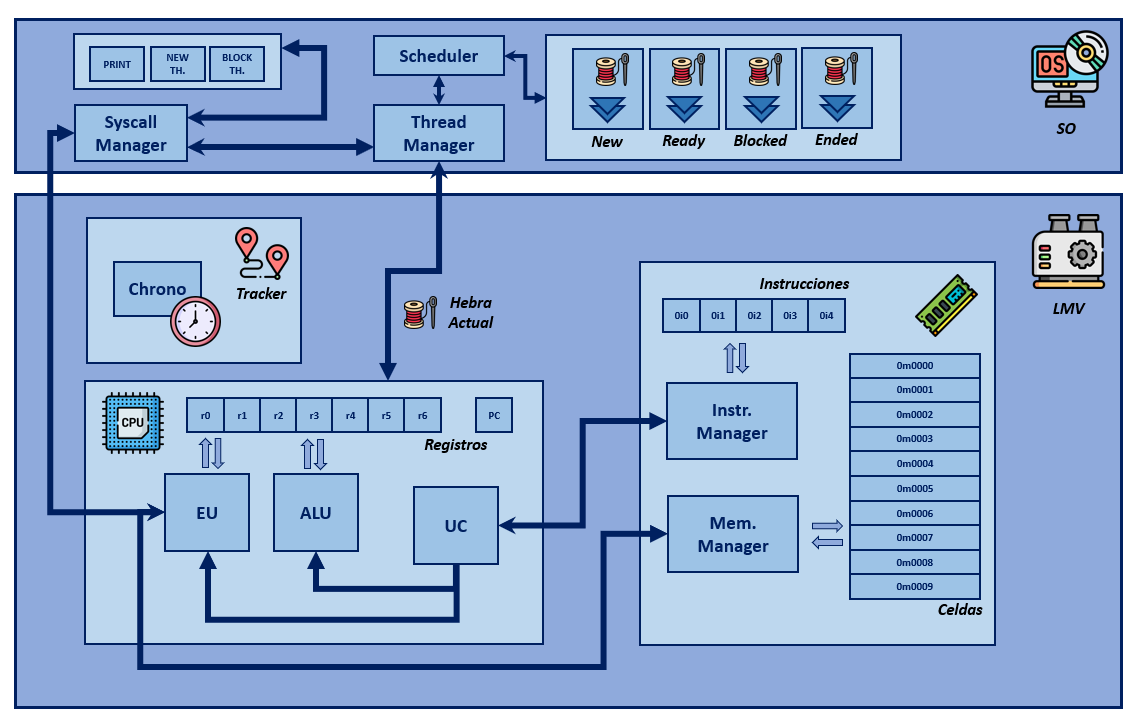
\includegraphics[width=\linewidth]{images/lmp/LVM_resume.png}
    \caption{Esquemático de la Máquina Virtual de Lamport}
    \label{fig:LVMResume}
\end{figure}

\begin{itemize}
    \item \textbf{CPU (~\ref{subsubsec:CPULVM} )}: El núcleo de procesamiento de la LVM. Aquí se realizan todas las operaciones aritméticas, lógicas y de control. Está compuesto por diversos registros que almacenan datos de manera temporal y un planificador de hebras para habilitar concurrencia.
    
    \item \textbf{Memoria (~\ref{subsec:memoryLVM} )}: Es el componente encargado de almacenar datos e instrucciones que el CPU puede recuperar y ejecutar. A través de su estructura subdividida y mecanismos como la tabla de segmentos, se busca optimizar el acceso y gestión de la información.

    \item \textbf{Sistema Operativo (~\ref{subsec:SOLVM} )}: Diseñado para gestionar eficientemente las llamadas al sistema y los recursos de la LVM. Este componente se encarga de la interfaz entre el ``hardware'' y el ``software', facilitando la ejecución de programas y la administración de memoria y procesos.
\end{itemize}

\subsection{CPU}\label{subsubsec:CPULVM}
La CPU de la Máquina Virtual de Lamport (LVM) es el componente encargado de ejecutar las instrucciones y gestionar las operaciones que se llevan a cabo dentro de la máquina. Actuando como el cerebro de la LVM, interpreta y lleva a cabo cada instrucción en la secuencia de comandos proporcionada, interactuando con otros componentes, como la memoria, para realizar cálculos, almacenar y recuperar datos, y gestionar el flujo de control.



\noindent
La CPU de la Máquina Virtual consta de los siguientes elementos:
\begin{itemize}
    \item \textbf{Vector de registros:} Un conjunto de almacenamientos temporales utilizados para mantener valores que la CPU puede necesitar rápidamente. Estos registros facilitan las operaciones aritméticas, lógicas y de movimiento de datos, permitiendo a la CPU acceder a información esencial sin tener que consultar la memoria principal constantemente.
    
    \item \textbf{Contador de programa:} También conocido como PC (Program Counter), es un registro especializado que apunta a la próxima instrucción que la CPU debe ejecutar. Avanza secuencialmente a medida que se ejecutan las instrucciones, pero puede cambiar de manera no secuencial durante saltos, bucles y llamadas a subprogramas.
    
    \item \textbf{Unidad Aritmético Lógica (ALU):} Esta unidad es responsable de llevar a cabo todas las operaciones matemáticas y lógicas en la CPU. Procesa las operaciones básicas como suma, resta, multiplicación, división y operaciones lógicas como AND, OR, NOT. Es esencial para la toma de decisiones y cálculos en la computadora.

    \item \textbf{Unidad de Control (UC):} Coordina las actividades de todas las partes de la máquina virtual. La UC interpreta las instrucciones del programa, convirtiéndolas en señales que activan otras partes de la CPU para ejecutarlas. Controla el flujo de datos dentro de la CPU y hacia/desde la memoria.

    \item \textbf{Unidad de Ejecución (EU):} Es la parte de la CPU donde efectivamente se realizan las instrucciones de los programas. La EU utiliza los datos e instrucciones proporcionados por la Unidad de Control para realizar las operaciones y manejar los registros.
\end{itemize}


Además la Unidad de Control de la CPU tiene acceso directo al vector de instrucciones generado en la fase de generación de código intermedio. El contador de programa apunta a \code{IR_START_PROGRAM}, y se van ejecutando las instrucciones que correspondan con la dirección a la que apunta el contador de programa.

\subsubsection{Registros}\label{subsubsec:registrosLVM}
Los registros es de las partes más importantes de la CPU en la máquina virtual, ya que albergan y gestionan los valores que las instrucciones de operación requieren para su ejecución, principalmente para tareas de consulta y modificación. Siguiendo el esquema de registros "infinitos" discutido en ~\ref{subsec:asignacionRegIR}, la estructura del vector de registros se organiza de la siguiente manera:
\begin{itemize}
    \item \textbf{Registros r0 - r30}: Registros dedicados a parámetros y variables locales de subprogramas.
    \item \textbf{Registro r31}: Registro dedicado al retorno de una función.
    \item \textbf{Registros r32 en adelante}: Registros de propósito general.
\end{itemize}

\subsection{Esquema de ejecución de código en LVM}
Finalmente, lo que queda es comentar cómo es el esquema general de ejecución de instrucciones IR en la Máquina Virtual de Lamport:

\begin{enumerate}
    \item Se crea la tabla de segmentos utilizando el contenido de las tablas de literales, variables y etiquetas, definiendo los segmentos y asignando las direcciones físicas correspondientes.
    \item Se invoca a la clase iniciadora de la memoria de la MV y vuelca el contenido inicial de las tablas a la memoria.
    \item La clase iniciadora a continuación crea todas las hebras que corresponden con procesos estáticos, con sus correspondientes atributos de inicialización como identificador, contador de programa, etc. Adicionalmente, se crea la hebra ``maestra'' encargada de inicializar la ejecución del programa además de ejecutar las instrucciones correspondientes a la asignación del valor de inicio de las variables globales en tiempo de ejecución. Finalmente, se vuelcan en la cola de hebras nuevas del planificador. 
    \item Se coloca el contador de programa en la instrucción \code{IR_START_PROGRAM} y la ejecución siempre empezará con la hebra maestra, que terminará su trabajo cuando consuma todo su quantum de tiempo definido en el paso de creación de hebras.
    \item Posteriormente, en cada ciclo de CPU se decide qué hebra es la que ejecuta el procesador a través del planificador.
    \item La hebra está ejecutando instrucciones hasta que el planificador decide cambiarla por otra, ya sea porque ésta cambió su estado o porque ya agotó su tiempo de CPU.
    \item Se finaliza el programa cuando se alcanza la instrucción \code{IR_END_PROGRAM} o cuando todos los procesos creados han terminado su ejecución.
\end{enumerate}

\subsection{Memoria}\label{subsec:memoryLVM}
La memoria en la Máquina Virtual de Lamport se implementa mediante una clase especializada que contiene un mapa ordenado. En este mapa, la clave representa la dirección física de memoria y el valor asociado es el contenido almacenado en dicha dirección, que consiste en un \textbf{bloque de memoria}, una abstracción sobre las celdas de memoria reales, permitiendo así poder alojar múltiples tipos de dato sin tener que preocuparse por reservar o liberar memoria explícitamente como en una máquina convencional. Esta estructuración permite un acceso rápido y organizado a los datos, emulando de manera efectiva el comportamiento de una memoria física en sistemas de hardware.

\subsubsection{Tabla de segmentos}\label{subsubsec:pageTableLVM}
La gestión de la memoria en la Máquina Virtual de Lamport se basa en un esquema segmentado. Cada segmento, en este contexto, representa una categoría específica de datos: literales, etiquetas, variables globales, índices, y un segmento específico para las variables locales de cada proceso. Para acceder a una entrada específica dentro de un segmento, se utilizan las direcciones virtuales. 


La \textit{tabla de segmentos} desempeña un papel crucial en el mecanismo de traducción de la Máquina Virtual de Lamport. Su principal función es mantener un registro de qué dirección lógica corresponde a qué dirección física en la memoria basándose en la segmentación. Así, cuando la máquina virtual requiere acceder a un dato en específico, consulta esta tabla para determinar su ubicación física correspondiente.


Por ejemplo, si se accede al segmento 0 (representando literales) y a la dirección virtual 0, se está refiriendo a la dirección física donde se encuentra almacenado el primer literal. Esta organización permite una gestión sistemática y estructurada de la memoria, facilitando el acceso y la asignación de memoria para diferentes tipos de datos.


Con este esquema, la máquina virtual se beneficia de una organización lógica clara, a la vez que mantiene la flexibilidad de asignar o reasignar direcciones físicas según las necesidades.


A continuación se especifican los segmentos definidos y los rangos de direcciones físicas asignados:

\begin{itemize}
    \item \textbf{Segmento 0 (literales):} Desde la dirección 0 hasta la dirección 999.
    \item \textbf{Segmento 1 (etiquetas):} Desde la dirección 1000 hasta la dirección 1999.
    \item \textbf{Segmento 2 en adelante (variable):} Desde la dirección 2000 en adelante. Aquí se definen múltiples segmentos consecutivos dependiendo de:
    \begin{itemize}
        \item Si hay variables globales (segmento 2).
        \item Si hay índices de bucles (segmento 3).
        \item Número de procesos (segmento 4 en adelante).
    \end{itemize}
\end{itemize}

El lector puede preguntarse qué sucedería si no hay suficientes direcciones físicas para cubrir un segmento completo. En ese caso, se ha optado por lanzar una excepción indicando que el programa no se puede ejecutar.

\subsubsection{Iniciador de la memoria}
En la fase de generación de código intermedio, específicamente en la tabla de variables, hay un campo denominado \textit{valor inicial}. Simplemente contiene el valor de inicio de la variable en función del tipo de dato, por ejemplo 0 para los enteros, o la cadena vacía para los strings. Teniendo en cuenta esto y el esquema de segmentación implementado anteriormente, se decidió desarrollar una clase encargada de volcar a memoria todo el contenido de todas las tablas en los bloques de memoria correspondientes a las direcciones físicas.

\subsection{Sistema Operativo}\label{subsec:SOLVM}
En el corazón de la máquina virtual de Lamport reside su sistema operativo simulado, una componente esencial que facilita la interacción entre el software y el hardware simulado. Este sistema operativo simulado desempeña funciones clave que son cruciales para el funcionamiento eficiente y realista de la máquina virtual, especialmente en lo que respecta a la gestión de procesos y recursos.

Una de las funciones principales de este sistema operativo es la captura y el manejo de llamadas al sistema. Esto incluye operaciones fundamentales como la impresión de contenido en pantalla, proporcionando una interfaz para que los programas en ejecución puedan comunicar resultados y estados al usuario. Este mecanismo simula la interacción entre aplicaciones y sistemas operativos reales, ofreciendo una experiencia auténtica y educativa para el usuario.

Además, el sistema operativo de la máquina virtual juega un papel vital en la gestión de la CPU, en particular en la coordinación con el planificador para tomar decisiones sobre la ejecución de hebras. Esto implica determinar qué hebra debe ejecutarse a continuación, una tarea que requiere un equilibrio cuidadoso entre eficiencia y equidad para asegurar que todos los procesos reciban tiempo de CPU adecuado. Esta simulación proporciona una visión práctica de cómo los sistemas operativos modernos manejan la planificación y ejecución de múltiples procesos y hebras.

Otras funciones críticas incluyen mecanismos de bloqueo y terminación de procesos. El sistema operativo simulado maneja situaciones en las que los procesos necesitan esperar por recursos o por la finalización de otras tareas, implementando así estrategias de bloqueo y señalización. Asimismo, gestiona la terminación de procesos, asegurando que los recursos se liberen adecuadamente y que el sistema se mantenga estable y eficiente.

\subsection{Estado de la memoria de LVM con ``HolaMundo''}
Se acerca el momento en el que el programa ``HolaMundo'' (~\ref{fig:lamportHolaMundo} ) podrá ser ejecutado como un lenguaje cualquiera, pero antes de ello se muestra la fase donde el contenido de las tablas de literales, variables y etiquetas definidas en ~\ref{fig:IRHolaMundo} se vuelca a la memoria de la máquina.


\noindent
Este es el resultado de la ejecución del iniciador de memoria:
\begin{verbatim}
==========================================================
TABLA DE SEGMENTOS
==========================================================
Segmento número (0) : literales
==========================================================
Dirección Virtual    Dirección Física    
==========================================================
0                     0m00000000            
1                     0m00000001            
2                     0m00000002            
3                     0m00000003            
4                     0m00000004            
5                     0m00000005            
6                     0m00000006            
==========================================================

Segmento número (1) : etiquetas
==========================================================
Dirección Virtual    Dirección Física    
==========================================================
0                     0m00001000            
1                     0m00001001            
2                     0m00001002            
3                     0m00001003            
4                     0m00001004            
5                     0m00001005            
6                     0m00001006            
==========================================================

Segmento número (2) : variables globales
==========================================================
Dirección Virtual    Dirección Física    
==========================================================
0                     0m00002000            
==========================================================

Segmento número (3) : indices
==========================================================
Dirección Virtual    Dirección Física    
==========================================================
==========================================================

Segmento número (4) : Main
==========================================================
Dirección Virtual    Dirección Física    
==========================================================
4                     0m00002001            
5                     0m00002002            
==========================================================

==========================================================
MEMORIA DE LA MÁQUINA VIRTUAL
==========================================================
Dirección            Tipo de bloque        Contenido             
==========================================================
0m00000000            string                "Hola ""             
0m00000001            string                "!"                 
0m00000002            integer               0                     
0m00000003            integer               18                    
0m00000004            string                "Daniel"            
0m00000005            integer               23                    
0m00000006            string                "El numero magico vale: "
0m00001000            instr. address        0i0001                
0m00001001            instr. address        0i0004                
0m00001002            instr. address        0i0013                
0m00001003            instr. address        0i0014                
0m00001004            instr. address        0i0022                
0m00001005            instr. address        0i0025                
0m00001006            instr. address        0i0042                
0m00002000            integer               0                     
0m00002001            string                ""                    
0m00002002            integer               0                     
\end{verbatim}
\begin{figure}[hbtp]
\caption{Programa ``¡Hola Mundo!'' Lamport: Tabla de segmentos y memoria de LVM en su estado inicial.}
\label{fig:preLVMHolaMundo}
\end{figure}

\subsection{Control de excepciones}
Como se mencionó en ~\ref{subsec:semanticaLamport}, el lenguaje Lamport es \textit{inseguro}. Esto pone en manos del programador la responsabilidad de garantizar la corrección de ciertas operaciones. Sin las debidas precauciones, el comportamiento del programa podría ser indeterminado. Esta circunstancia destaca la necesidad de implementar un mecanismo de \textit{excepciones}.


Una excepción juega un papel crucial en la gestión de errores y situaciones inesperadas durante la ejecución de un programa. Sirve como mecanismo de señalización que indica que algo ha ido mal o que ha surgido una condición no prevista.


\noindent
La Máquina Virtual de Lamport es capaz de tratar dos tipos de excepciones:
\begin{itemize}
    \item \textbf{Excepción ZeroDivision:} Se produce cuando se intenta realizar una operación de división, cuyo segundo operando (divisor) es el número 0.
    \item \textbf{Excepción OutOfBounds:} Se produce cuando se intenta relizar un acceso indebido a un array, esto es, una posición fuera de los límites que le corresponden.
\end{itemize}

\section{Hebras y planificación}
Dado que el motivo principal de este proyecto es \textit{simular concurrencia}, se ha considerado pertinente dedicar este espacio específico para tratar en profundidad la implementación y gestión de hebras, así como el mecanismo de planificación que las coordina. A continuación, se detallan los mecanismos y estrategias adoptadas para lograr una simulación fiel y eficiente de la concurrencia en la Máquina Virtual.

\subsection{Tipos de hebras}
En la Máquina Virtual hay diferentes tipos de hebras dependiendo de su naturaleza, enumerándose a continuación:

\begin{itemize}
    \item \textbf{Iniciadora}. Es una hebra especial que se crea una única vez, al inicio del programa. Su misión es inicializar las variables globales si las hay. Acto seguido, se destruye y se empieza el ciclo de CPU con las hebras de proceso.
    \item \textbf{Estáticas}. Estas hebras son aquellas que corresponden a un proceso de Lamport y están definidas desde el inicio del programa. Su existencia y características se determinan en tiempo de traducción, y no varían durante la ejecución del programa.
    \item \textbf{Dinámicas:} Son hebras creadas en tiempo de ejecución, dependiendo del flujo y las condiciones del programa. Un claro ejemplo de la creación de una hebra dinámica es cuando se ejecuta una instrucción del tipo \code{fork}. Estas hebras ofrecen una gran flexibilidad, adaptándose a las necesidades y circunstancias que surgen durante la ejecución del programa.
\end{itemize}

\subsection{Implementación de hebras}
En el contexto del lenguaje Lamport, una hebra se define como la unidad mínima de ejecución, esencialmente representando un hilo de control dentro de un programa. Cada hebra comprende la ejecución de un conjunto específico de instrucciones, pudiendo operar de manera independiente pero compartiendo ciertos recursos con otras hebras del mismo proceso. Esta independencia permite que diferentes hebras gestionen tareas distintas en paralelo, maximizando la utilización de los recursos y permitiendo un diseño más modular y eficiente de los programas.



\noindent
Las hebras se componen de los siguientes elementos:
\begin{itemize}
    \item Identificador de la hebra.
    \item Estado actual de la hebra.
    \item Segmento de direcciones de memoria.
    \item Vector de registros propios.
    \item Pila de ejecución para llamadas a subprogramas.
    \item Contador de instrucciones ejecutadas.
    \item Quantum de hebra.
    \item Contador de hebras hijas.
\end{itemize}


\noindent
En el caso de que se trate de una hebra hija, es decir, una hebra dinámica creada desde otra hebra, ésta contiene la referencia al proceso padre que la creó. Es especialmente importante que la hebra hija siempre notifique de sus cambios de estado a su padre, puesto que los mecanismos de sincronización en su mayoría de casos se tratan de una comunicación adecuada entre estos dos tipos de hebras.

\subsection{El modelo de 5 estados para Hebras}

El modelo de 5 estados representa un marco conceptual que permite entender y categorizar las diferentes etapas o fases por las que una hebra puede pasar durante su ciclo de vida. Cada estado ofrece una perspectiva única sobre la condición y actividad de la hebra. A continuación, se describen brevemente estos cinco estados:

\begin{enumerate}
    \item \textbf{Nuevo (New):} En este estado, la hebra ha sido creada pero aún no ha comenzado su ejecución. Está esperando la asignación de recursos necesarios para iniciar.

    \item \textbf{Listo (Ready):} La hebra está lista para ejecutarse y está esperando ser asignada a un procesador por el planificador. Todos los recursos necesarios ya han sido asignados, pero la hebra no está siendo ejecutada en este momento.

    \item \textbf{En ejecución (Running):} La hebra ha sido asignada a un procesador y está siendo ejecutada actualmente. En este estado, la hebra realiza sus tareas designadas.

    \item \textbf{Bloqueado (Blocked):} Aquí, la hebra está esperando un evento o recurso específico para continuar. Puede estar esperando la conclusión de una operación de I/O, la liberación de un recurso, o cualquier otro evento que impida su ejecución continua.

    \item \textbf{Terminado (Terminated):} La hebra ha completado su ejecución y ha finalizado todas sus tareas. Una vez que una hebra alcanza este estado, no puede regresar a los estados anteriores.
\end{enumerate}

Este modelo proporciona una estructura clara para visualizar y entender el flujo y transiciones que una hebra experimenta, facilitando la gestión y control de la concurrencia en sistemas informáticos.

\begin{figure}[h]
    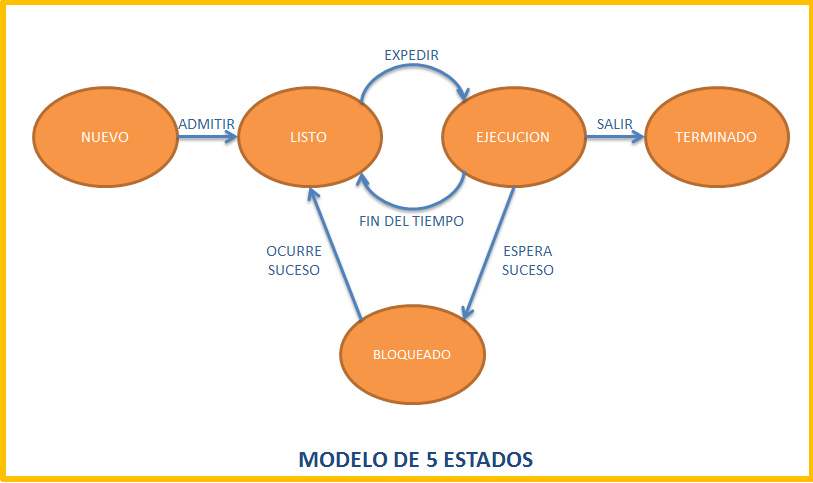
\includegraphics[width=\linewidth]{images/implementacion/hebras/modelo5_estados.png}
    \caption{Modelo de 5 estados para hebras. Diagrama de transiciones.}
    \label{fig:modelo_estados_hebras}
\end{figure}

\newpage

\subsection{Planificador. Esquema Round-Robin con Quantums aleatorios}
El esquema Round-Robin con Quantums aleatorios presenta una innovadora variante del tradicional algoritmo Round-Robin, adaptándose de manera dinámica a las condiciones del sistema y buscando un equilibrio entre la equidad y el rendimiento.



El concepto de \textit{quantum} se refiere al tiempo máximo que una hebra puede pasar en estado de ejecución antes de que se le obligue a ceder el procesador a otra hebra en espera. En el contexto de la planificación Round-Robin, el quantum es simplemente el tiempo asignado a cada hebra para su ejecución antes de pasar al siguiente en la cola, que en este caso se mide como ``\textit{número de instrucciones permitidas para ejecutar}''. Si una hebra no finaliza su ejecución durante su quantum, se coloca al final de la cola de hebras listas y espera su próximo turno. En este enfoque particular, donde el quantum es aleatorio, se introduce un factor de variabilidad que puede ayudar a optimizar la asignación de recursos en función de las condiciones dinámicas del sistema.



\noindent
El planificador consta de los siguientes elementos:
\begin{itemize}
    \item Una cola de hebras nuevas.
    \item Una cola de hebras listas.
    \item Una cola de hebras bloqueadas.
    \item Una cola de hebras terminadas.
    \item Un puntero a la hebra que está actualmente ejecutando.
    \item Un mapa de semáforos con sus respectivas colas de hebras bloqueadas: El planificador está equipado con métodos para invocar las operaciones \code{wait} y \code{signal}, gestionando internamente las hebras que quedan bloqueadas por la acción de estos semáforos.
\end{itemize}



Finalmente, se describe el esquema de planificación Round-Robin definido para la simulación de la concurrencia entre hebras:
\begin{enumerate}
    \item Si se trata de la primera ejecución del planificador, todas las hebras de procesos se encuentran en la cola de nuevas. En ese caso:
    \begin{enumerate}
        \item Se mueven todas las hebras de la cola de nuevas a la cola de listas.
        \item Se baraja la cola de hebras y se saca la que se quedó en el frente de cola, y se marca para ejecución.
    \end{enumerate}
    \item En el resto de ejecuciones:
    \begin{enumerate}
        \item Si sólo hay una hebra activa en el sistema, se le cede el control de la CPU indefinidamente. No hay nada que planificar.
        \item Si hay más hebras en el sistema:
        \begin{enumerate}
            \item Se comprueba si hay hebras nuevas, y en ese caso se mandan todas a la cola de listas.
            \item Se comprueba si la actual ha terminado.
            \begin{enumerate}
                \item En caso afirmativo, la hebra se envía a la cola de terminadas. Además, si la hebra en cuestión es hija de un padre, se le notifica.
                En ese mismo punto, se intenta desbloquear al padre, sólo si todas sus hijas terminaron, incluyendo la que se acaba de marcar.
                \item Si no ha terminado pero ha excedido su quantum, se manda la hebra actual a la cola de listas y se trae otra del frente de esa misma cola para ejecutar.
                \item Si no ha termiando y puede seguir ejecutando instrucciones, simplemente continua teniendo el control de CPU.
            \end{enumerate}
        \end{enumerate}
    \end{enumerate}
\end{enumerate}

Indicar además que, cuando una hebra pasa de lista a ejecutando, se le asigna un quantum aleatorio de entre \textbf{1 y 4 instrucciones}.

\section{Gesitón de señales de interrupción UNIX (POSIX)}\label{sec:posixSignalsLMP}
En el desarrollo de la Máquina Virtual de Lamport, se ha implementado un mecanismo de gestión de señales de interrupción UNIX, siguiendo el estándar POSIX, con especial atención a la señal de interrupción Ctrl+C (SIGINT). Este mecanismo desempeña un papel crucial en la operación segura y controlada de la máquina virtual, especialmente en situaciones de bloqueo o ejecución de bucles infinitos.

La interrupción Ctrl+C es una señal común en los entornos de sistemas operativos UNIX para solicitar la terminación de un proceso en ejecución. En el contexto de la Máquina Virtual de Lamport, esta señal ha sido configurada para funcionar como un mecanismo de detención segura. Al detectar la señal de interrupción, la máquina virtual inicia un proceso de cierre ordenado, asegurando que todos los recursos y procesos en ejecución se gestionen adecuadamente antes de la terminación.

La implementación de este mecanismo de gestión de señales no solo mejora la robustez de la Máquina Virtual de Lamport, sino que también enriquece la experiencia del usuario al proporcionar una forma efectiva y segura de manejar situaciones inesperadas durante la ejecución del programa. Además, alinea la máquina virtual con las prácticas estándar en entornos UNIX, facilitando su integración y uso en estos sistemas.

\section{Interfaces de control de intérprete: ``LMP Utils``}\label{sec:implementacionLMPUtils}
Hasta ahora se han definido y desarrollado una gran cantidad de módulos que se comunican entre sí de varias formas. Es por ello por lo que es necesario establecer una vía de control de forma sencilla y unificada entre cada módulo y la función principal del intérprete que es quien ejecuta todos los analizadores y clases en el orden que corresponde. En total se han definido un total de 5 controladores diferentes:

\begin{itemize}
    \item \textbf{Controlador de flujos de E/S:} Es el encargado de realizar el tratamiento de apertura y cierre del fichero de código Lamport a ejecutar.
    \item \textbf{Controlador de Análisis:} Es el encargado de ejecutar los analizadores sintáctico y semántico, y de mantener el AST del programa, enviando al intérprete los errores en caso de que se produzcan.
    \item \textbf{Controlador de IR:} Es el encargado de llamar al optimizadador de AST y constructor de instrucciones de código intermedio.
    \item \textbf{Controlador de LVM:} Es el encargado de lanzar la máquina virtual cuando se ha generado el código intermedio.
    \item \textbf{Controlador de registros de eventos (logging):} Este controlador es especial y extremadamente útil para el usuario del intérprete. Su función es registrar todos los eventos que se han producido en el intérprete, desde el análisis sintáctico pasando a la generación de código intermedio, estado de la memoria de la LVM y traza de ejecución, o la generación de errores.

    Genera un directorio denominado \code{log/} que contiene los ficheros de logging siguientes:
    \begin{itemize}
        \item \textbf{logging de AST}: Contiene el AST generado para el programa.
        \item \textbf{logging de IR}: Contiene las tablas de literales, variables y etiquetas, y el listado de instrucciones IR.
        \item \textbf{logging de LVM}: Contiene la tabla de segmentos y el estado de la memoria en el inicio de la máquina lamport, además de la traza de ejecución de la máquina al terminar. Además, también genera un fichero de registro con toda la traza de ejecución del programa en la Máquina Virtual.
        \item \textbf{logging de errores}: Contiene el listado de errores producidos en el análisis.
    \end{itemize}
\end{itemize}

\section{Ejecución de ``HolaMundo''}
Se ha llegado al final del proyecto, donde por fin se puede ejecutar el programa ``HolaMundo'' (~\ref{fig:lamportHolaMundo} ) del que tantas veces se ha hablado a lo largo de estas secciones. 


\noindent
El resultado de la ejecución es el siguiente:
\begin{figure}[h]
  \begin{minipage}{\linewidth}
    \centering
    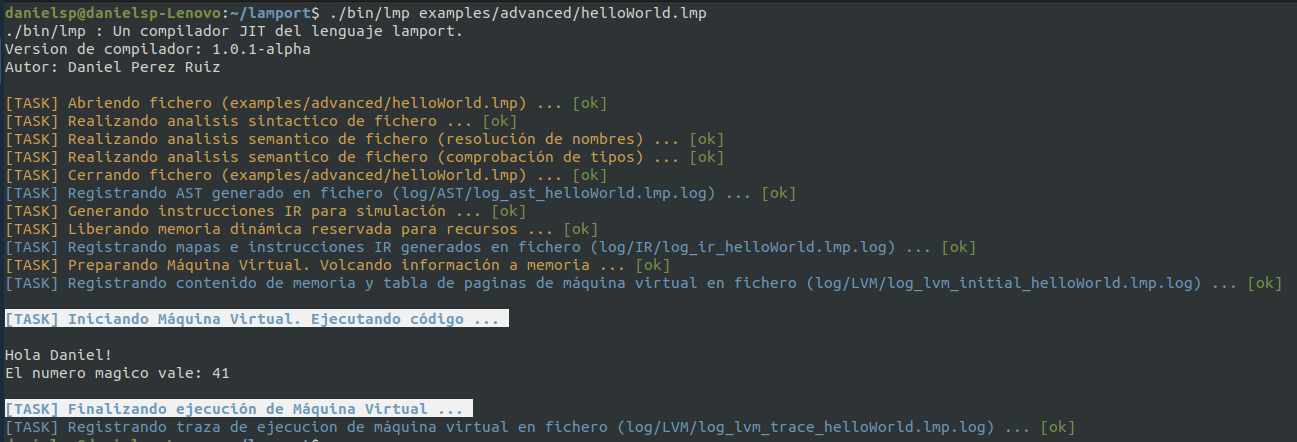
\includegraphics[width=\linewidth]{images/implementacion/ejecucion/lmp_hola_mundo.png}
    \caption{Ejecución de ``HolaMundo'' en el intérprete.}
    \label{fig:ejecucionHolaMundo}
  \end{minipage}
  \vspace{10pt} 
  \begin{minipage}{\linewidth}
    \centering
    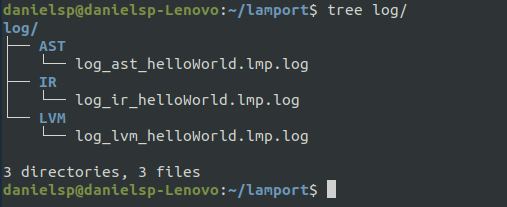
\includegraphics[width=\linewidth]{images/implementacion/ejecucion/logs.png}
    \caption{Ficheros de logging generados tras la ejecución.}
    \label{fig:logsHolaMundo}
  \end{minipage}
\end{figure}

\newpage
\subsection{Traza de ejecución de ``HolaMundo''}
Al finalizar la máquina virtual, se genera un fichero de registro con todas las operaciones que ésta ha ido realizando a nivel de CPU, de memoria, y de llamadas al sistema operativo. En la siguiente imagen se muestra la cabecera de la traza de ejecución para el programa ``HolaMundo'':
\begin{figure}[h]
  \begin{minipage}{\linewidth}
    \centering
    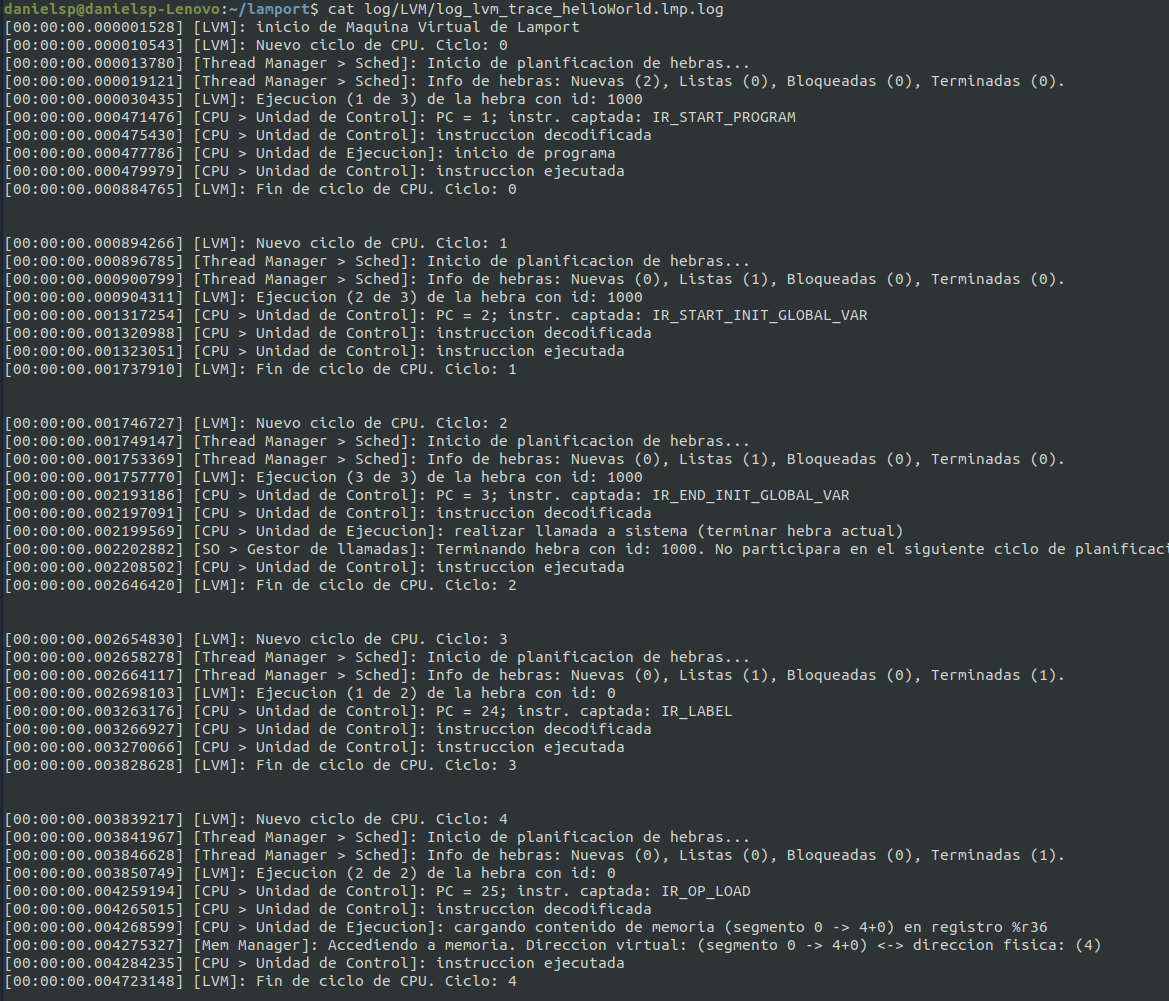
\includegraphics[width=\linewidth]{images/implementacion/ejecucion/traza.png}
    \caption{Traza de ejecución de ``HolaMundo''.}
    \label{fig:trazaHolaMundo}
  \end{minipage}
\end{figure}

\newpage
\section{Dockerización del intérprete}
Con la evolución constante de la tecnología y las infraestructuras de software, la necesidad de crear aplicaciones portables y escalables ha cobrado mayor importancia. Docker, una herramienta que permite la creación de contenedores, surge como una solución a esta demanda. Un contenedor Docker encapsula una aplicación junto con todas sus dependencias en una unidad estándar de software, garantizando que la aplicación se ejecute de la misma manera sin importar dónde se despliegue. 



En el contexto del intérprete desarrollado, la dockerización ofrece ventajas significativas en términos de portabilidad, aislamiento y replicabilidad. Esta sección detallará el proceso y las consideraciones adoptadas al dockerizar el intérprete, permitiendo su distribución y ejecución de manera homogénea en diferentes entornos.

\subsection{Construcción del contenedor}
Para construir el contenedor Docker que encapsulará el intérprete junto con todas sus dependencias, se han realizado las siguientes tareas:

\begin{enumerate}
    \item Elección de una imagen base. Ésta debe ser del menor tamaño posible para que sólo contenga lo imprescindible, además de ser una imagen que reciba constantes actualizaciones de seguridad y mantenimiento. En el caso de este proyecto, \textbf{alpine} es una excelente elección por cumplir estas dos características.
    \item Construir el fichero \code{Dockerfile}. Este fichero indica cómo se debe construir el contenedor de forma automática, aprovisionándolo de todas las dependencias.
    \item Definir script de ejecución utilizando el contenedor virtual. Para hacer aún más fácil el uso de esta herramienta se definió un script denominado \code{./lmp_docker.sh} que ejecuta el contenedor utilizando como argumento el fichero de código Lamport indicado.
\end{enumerate}

\subsection{Compilación estática del intérprete}
La compilación estática se refiere al proceso de integrar todas las bibliotecas y dependencias requeridas por una aplicación directamente en el binario ejecutable, en lugar de depender de bibliotecas compartidas en el sistema en tiempo de ejecución. Este método tiene varias ventajas, especialmente en el contexto que concierne a esta sección:

\begin{itemize}
\item \textbf{Portabilidad mejorada}: Un binario estáticamente enlazado no tiene dependencias externas, lo que garantiza que funcionará en cualquier entorno que lo ejecute, eliminando así problemas relacionados con versiones de bibliotecas o dependencias faltantes.
\item \textbf{Reducción del tamaño del contenedor}: Al no requerir la instalación de bibliotecas adicionales en el contenedor (sólo se necesita instalar flex y bison de manera inevitable), el tamaño de la imagen resultante puede reducirse significativamente. En este proyecto, la imagen del contenedor se redujo de 249 MB a tan solo 24 MB, una optimización impresionante.
\item \textbf{Seguridad mejorada}: Al reducir el número de componentes en el contenedor, se disminuye la superficie de ataque potencial, al eliminar software adicional que no es esencial para la aplicación pero que podría presentar vulnerabilidades.
\end{itemize}

Para lograr la compilación estática del intérprete, se utilizaron las herramientas gcc y g++ con las opciones de enlazado estático. Además, se aprovechó el enfoque de construcción multi-etapa en Docker, donde la primera etapa incluye todas las herramientas y dependencias necesarias para la compilación, y la segunda etapa simplemente copia el binario resultante, resultando en una imagen Docker final limpia y optimizada.

\begin{figure}[h]
    \begin{adjustbox}{center}
        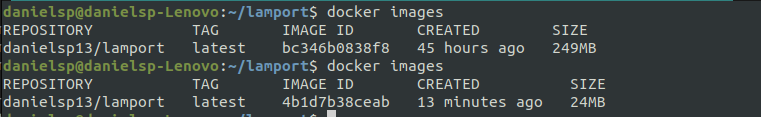
\includegraphics[width=\linewidth]{images/implementacion/docker/docker_reduce.png}
    \end{adjustbox}
    \caption{Tamaño de contenedor docker antes y después de usar compilación estática.}
    \label{fig:DockerReduce}
\end{figure}

	% Conclusiones
	\chapter{\textbf{Programas escritos en Lamport}}
En este capítulo se definen algunos ejemplos de programas escritos en el lenguaje Lamport y su resultado de ejecución, con el objetivo de mostrar el correcto funcionamiento del intérprete:

\section{Ejemplos secuenciales}
Los siguientes ejemplos mostrados aquí no necesitan de concurrencia para funcionar, pues siguen la estructura y sintaxis básica de cualquier otro programa desarrollado en cualquier lenguaje de alto nivel convencional:

\subsection{Ejemplo 1: Operaciones aritméticas}
\begin{lstlisting}[style=lamportStyle]
{Programa: arithmetic_operations.lmp}
{Autor: Daniel Perez Ruiz}

program Operaciones;
	var num1 : integer := (-4 + 6) * 10 - 2;
	var num2 : real := 3.0;

process Main;
	var num3 : integer := 5;
	var num4 : real := (3.5 * 4.2) + (6.7 - 2.3) / 1.1;
begin
	print("num1 tiene de valor: ",num1);
	print("num3 tiene de valor: ",num3);
	print("");
	
	print("num1 + num3 = ",num1+num3);
	print("num1 - num3 = ",num1-num3);
	print("num1 * num3 = ",num1*num3);
	print("num1 / num3 = ",num1/num3);
	print("num1 % num3 = ",num1%num3);
	print("-num1 = ",-num1);
	
	print("");
	
	print("num2 tiene de valor: ",num2);
	print("num4 tiene de valor: ",num4);	
	print("");
	
	print("num2 + num4 = ",num2+num4);
	print("num2 - num4 = ",num2-num4);
	print("num2 * num4 = ",num2*num4);
	print("num2 / num4 = ",num2/num4);
	print("-num4 = ",-num4);
	
end
\end{lstlisting}
\begin{figure}[h]
\caption{Programa Lamport: operaciones aritméticas}
\label{fig:lamportArithmeticOperations}
\end{figure}

\newpage
\begin{figure}[h]
    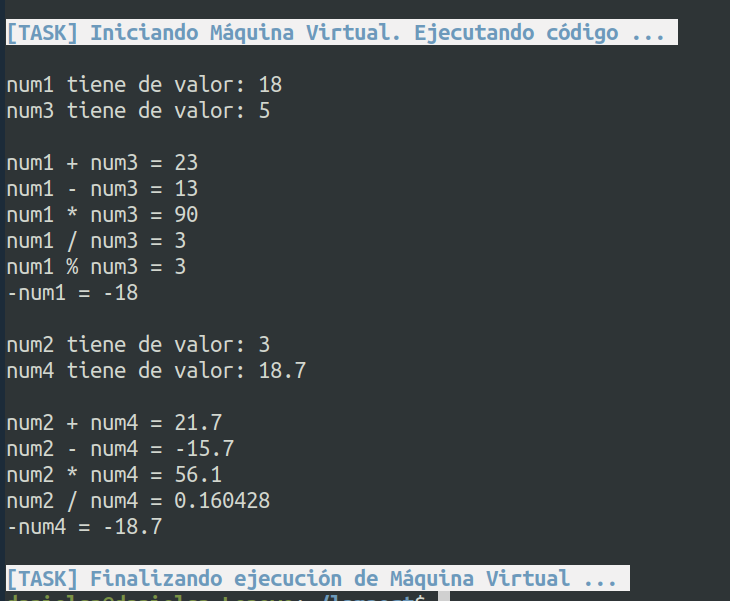
\includegraphics[width=\linewidth]{images/ejemplos/arithmeticOperations.png}
    \caption{Ejecución de programa: operaciones aritméticas.}
    \label{fig:lamportArithmeticOperations_exec}
\end{figure}

\newpage
\subsection{Ejemplo 2: Operaciones lógicas}
\begin{lstlisting}[style=lamportStyle]
{Programa: logical_operations.lmp}
{Autor: Daniel Perez Ruiz}

program Operaciones;
	var a : boolean := true;
	var b : boolean := false;

process Main;
	var c : boolean := true;
begin
	print("a es: ",a);
	print("b es: ",b);
	print("c es: ",c);
	print("");
	
	print("a y b es: ",a and b);
	print("a y c es: ",a and c);
	print("a y b y c es: ",a and b and c);
	print("");
	
	print("a o b es: ",a or b);
	print("a o c es: ",a or c);
	print("a o b o c es: ",a or b or c);
	print("");
	
	print("(a o b) y c es: ", (a or b) and c);
	print("(a o c) y b es: ", (a or c) and b);
	print("");
	
	print("no a es: ",not a);
	print("no b es: ",not b);
	
end
\end{lstlisting}
\begin{figure}[h]
\caption{Programa Lamport: operaciones lógicas}
\label{fig:lamportLogicalOperations}
\end{figure}

\newpage
\begin{figure}[h]
    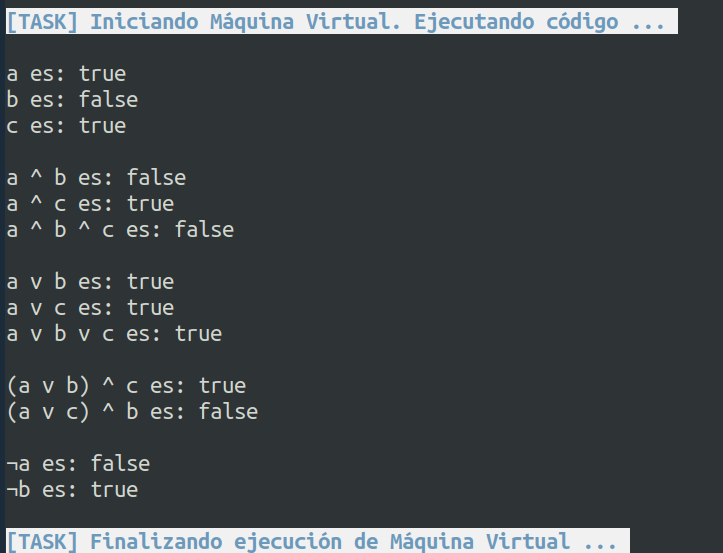
\includegraphics[width=\linewidth]{images/ejemplos/logical_operations.png}
    \caption{Ejecución de programa: operaciones lógicas.}
    \label{fig:lamportLogicalOperations_exec}
\end{figure}

\newpage
\subsection{Ejemplo 3: If/Else}
\begin{lstlisting}[style=lamportStyle]
{Programa: ifelse.lmp}
{Autor: Daniel Perez Ruiz}

program CompruebaEdad;
	var nombre1 : string := "Jorge";
	var edad1 : integer := 17;
	
	var nombre2 : string := "Pablo";
	var edad2 : integer := 22;
	
process main;
	var minimaEdad : integer := 18;
begin
	print(nombre1, ", tu edad es: ",edad1,". Comprobando si puedes entrar...");
	
	if edad1 < minimaEdad then
		begin
			print("NO puedes entrar. Debes tener ",minimaEdad," para poder entrar.");
		end
	else
		begin
			print("Adelante!!. Puedes entrar");
		end
		
	print("");
		
	print(nombre2, ", tu edad es: ",edad2,". Comprobando si puedes entrar...");
	
	if edad2 < minimaEdad then
		begin
			print("NO puedes entrar. Debes tener ",minimaEdad," para poder entrar.");
		end
	else
		begin
			print("Adelante!!. Puedes entrar");
		end
end
\end{lstlisting}
\begin{figure}[h]
\caption{Programa Lamport: flujos de control if/else.}
\label{fig:lamportIfElse}
\end{figure}

\newpage
\begin{figure}[h]
    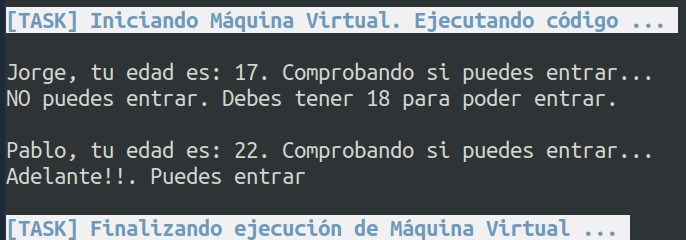
\includegraphics[width=\linewidth]{images/ejemplos/if_else.png}
    \caption{Ejecución de programa: if/else.}
    \label{fig:lamportIfElse_exec}
\end{figure}

\newpage
\subsection{Ejemplo 4: For}
\begin{lstlisting}[style=lamportStyle]
{Programa: for.lmp}
{Autor: Daniel Perez Ruiz}

program Bucles
	var contador : integer := 5;

process main;
	var startFor : integer := 1;
	var endFor : integer := 5;
begin
	print("La variable contador empieza en: ",contador);
	print("");
	print("Bucle for empieza en: ",startFor);
	print("Bucle for acaba en: ",endFor);
	
	print("");
	
	for i := startFor to endFor do
	begin
		contador := contador+1;
		print("--- contador vale ahora: ",contador);
		print("--- i vale: ", i);
	end
	
	print("");
	print("Ejecutando bucles anidados ...");
	print("");
	
	for j := 1 to 3 do
	begin
		print("------ j vale: ",j);
		for k := j to 4 do
		begin
			print("--- k vale: ",k);
		end
		print("");
	end
	
end
\end{lstlisting}
\begin{figure}[h]
\caption{Programa Lamport: bucles for.}
\label{fig:lamportFor}
\end{figure}

\newpage
\begin{figure}[!h]
    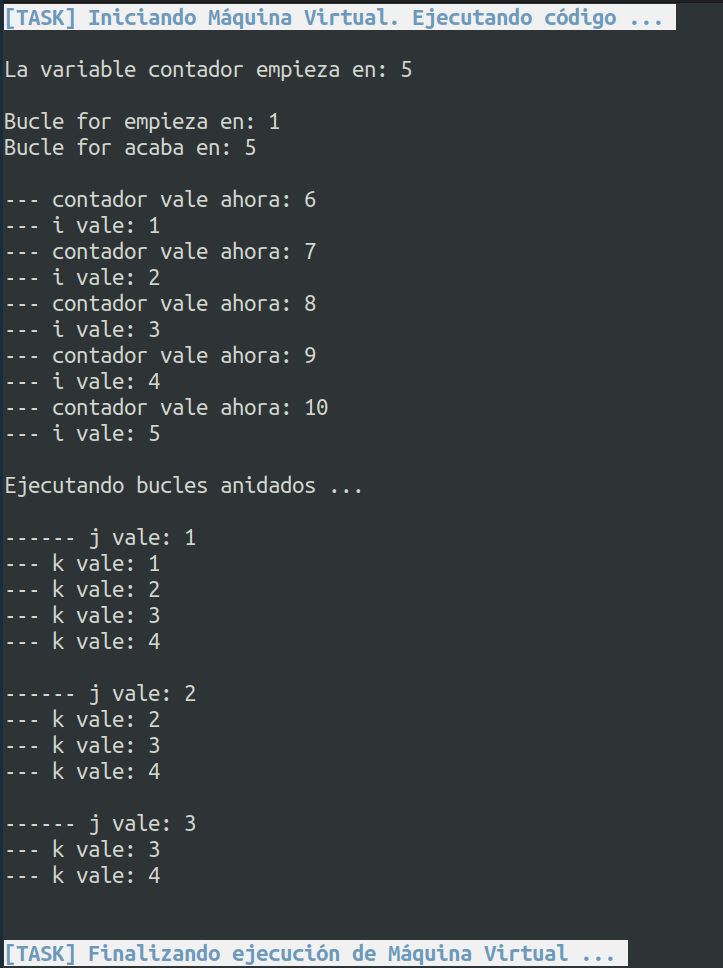
\includegraphics[scale=0.5]{images/ejemplos/for.png}
    \caption{Ejecución de programa: bucles for.}
    \label{fig:lamportFor_exec}
\end{figure}

\newpage
\subsection{Ejemplo 5: While}
\begin{lstlisting}[style=lamportStyle]
{Programa: while.lmp}
{Autor: Daniel Perez Ruiz}

program Bucles
	var contador : integer := 5;

process main;
	var valorMaximo : integer := 10;
begin
	print("La variable contador empieza en: ",contador);
	print("Su valor maximo debe ser: ",valorMaximo);
	print("");
	
	while contador < valorMaximo do
	begin
		contador := contador + 1;
		print(" --- Contador vale ahora: ", contador);
	end
	
	print(""); print("Fin de bucle");
end
\end{lstlisting}
\begin{figure}[h]
\caption{Programa Lamport: bucles while.}
\label{fig:lamportWhile}
\end{figure}

\newpage
\begin{figure}[h]
    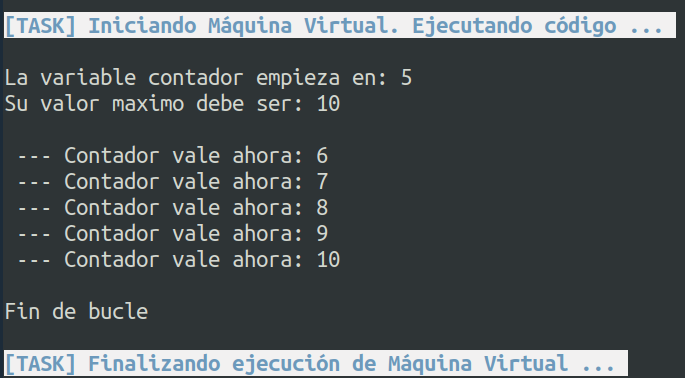
\includegraphics[width=\linewidth]{images/ejemplos/while.png}
    \caption{Ejecución de programa: bucles while.}
    \label{fig:lamportWhile_exec}
\end{figure}

\newpage
\subsection{Ejemplo 6: Uso de arrays}
\begin{lstlisting}[style=lamportStyle]
{Programa: for.lmp}
{Autor: Daniel Perez Ruiz}

program Arrays
	var numeros : array [5] integer;
process main;
	var letras : array [3] char;
begin
	print("Asignando numeros pares a array de numeros...");
	for i := 0 to 4 do
	begin
		print("Asignando a numeros[",i,"] el valor ",2*i);
		numeros[i] := 2*i;
	end
	
	print("");
	print("Imprimiendo array de numeros...");
	for j := 0 to 4 do
	begin
		print("numeros[",j,"] = ",numeros[j]);
	end
	
	letras[1] := 'd';
	print("");
	print("letras[1] es : ",letras[1]);
end
\end{lstlisting}
\begin{figure}[h]
\caption{Programa Lamport: uso de arrays}
\label{fig:lamportArray}
\end{figure}

\newpage
\begin{figure}[h]
    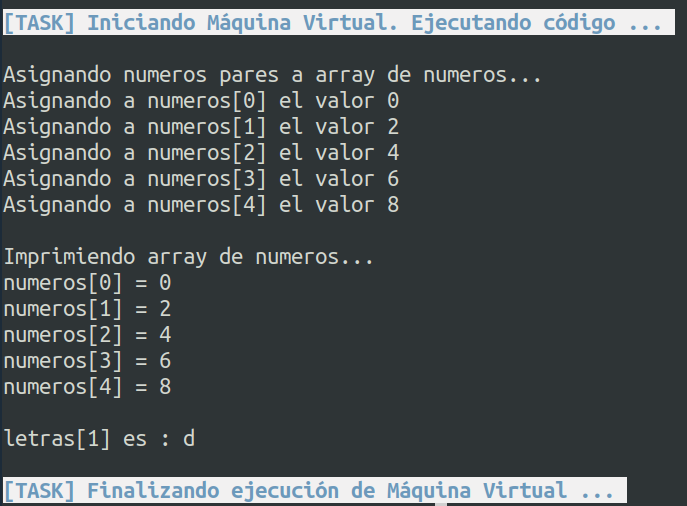
\includegraphics[width=\linewidth]{images/ejemplos/array.png}
    \caption{Ejecución de programa: arrays.}
    \label{fig:lamportArray_exec}
\end{figure}

\newpage
\section{Ejemplos que lanzan errores}
Los siguientes ejemplos mostrados son incorrectos, ya sean sintáctica o semánticamente, por lo que el intérprete lanzará los pertinentes mensajes de error.

\subsection{Ejemplo 1: Errores sintácticos en declaraciones}
\begin{lstlisting}[style=lamportStyle]
{Fichero: err_syntax_declarations.lmp}
{Autor: Daniel Perez Ruiz}
{Descripcion: Errores sintacticos de declaraciones}

program SyntaxErrors
	{CORRECTO}
	var v1 : integer;
	var v2 : string := "Hola";
	{ERROR}
	v3 : real;
	var 4v : boolean;
	var v5 char;
	var v6: string

process Main;
	{ERROR}
	var v7 : inventado;
	var v9 : array [5] invent;
	var v10 : integer := ;
	var v11 : integer 2+3;
	var v12 : integer := 1
begin
	print("Syntax errors!");
end
\end{lstlisting}
\begin{figure}[h]
\caption{Programa Lamport: errores sintácticos en declaraciones}
\label{fig:lamportErrSintaxDecl}
\end{figure}

\newpage
\begin{figure}[h]
    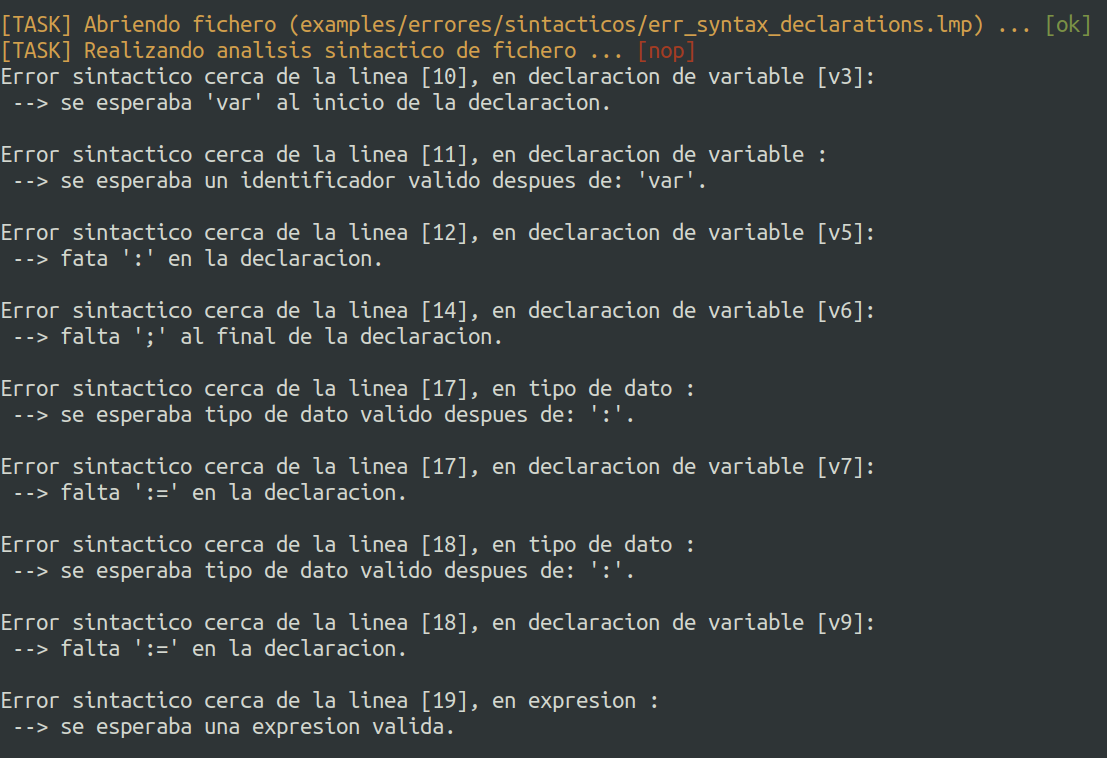
\includegraphics[width=\linewidth]{images/ejemplos/err_syntax/declarations.png}
    \caption{Ejecución de programa: errores sintácticos en declaraciones.}
    \label{fig:lamportErrSintaxDecl_exec}
\end{figure}

\newpage
\subsection{Ejemplo 2: Errores sintácticos en procedimientos}
\begin{lstlisting}[style=lamportStyle]
{Fichero: err_syntax_procedure.lmp}
{Autor: Daniel Perez Ruiz}
{Descripcion: Errores sintacticos de procedimientos}

program SyntaxErrors

{CORRECTO}
procedure imprimeEdad(a : string, b : integer);
begin
	print("Hola ",a,", tu edad es: ",b);
end

{CORRECTO}
procedure saluda();
begin
	print("hola");
end

{ERROR}
procedure proc1()
begin
	print("proc1");
end

{ERROR}
procedure 2proc();
	var v2 : invent;
begin
	print("fallo");
end

{ERROR}
procedure proc3(a : integer)
begin
	print("valor: ",a);
end

{ERROR}
procedure proc4(2 : integer);
begin
	print("fallo");
end

{ERROR}
procedure proc5(a char);
begin
	print("fallo");
end

{ERROR}
procedure proc6(a : invent);
begin
	print("fallo");
end

{ERROR}
procedure proc7(a : integer, b : invent);
begin
	print("fallo");
end

{ERROR}
procedure proc8(a : char,);
begin
	print("fallo");
end

process Main;
	{ERROR}
	var v1 : invent;
begin
	print("Syntax Errors!");
end
\end{lstlisting}
\begin{figure}[h]
\caption{Programa Lamport: errores sintácticos en procedimientos}
\label{fig:lamportErrSintaxProcedure}
\end{figure}

\newpage
\begin{figure}[h]
    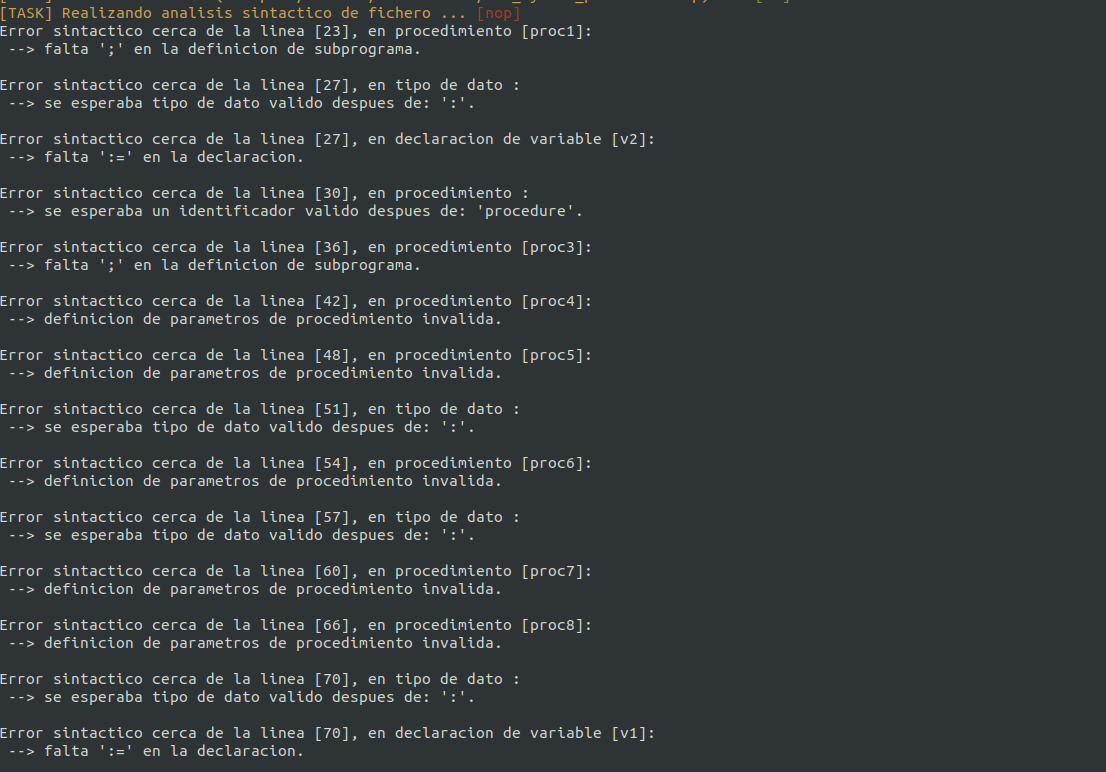
\includegraphics[width=\linewidth]{images/ejemplos/err_syntax/procedures.png}
    \caption{Ejecución de programa: errores sintácticos en procedimientos.}
    \label{fig:lamportErrSintaxProcedure_exec}
\end{figure}

\newpage
\subsection{Ejemplo 3: Errores semánticos: uso de variable no definida}
\begin{lstlisting}[style=lamportStyle]
{Fichero: undef_variable.lmp}
{Autor: Daniel Perez Ruiz}
{Descripcion: Contiene un error semantico de tipo: uso de variables no definidas}

program OperaEnteros

function suma(a: integer, b: integer) : integer;
begin
	{ERROR: Uso de variable no definida: resultadoSuma}
	resultadoSuma := a+b;
	return resultadoSuma;
end

procedure resta(a: integer, b: integer);
	var resultado : integer;
begin
	{ERROR: Uso de variable no definida: c}
	resultado := a - c;
	print(resultado);
end

process Main;
begin
	{ERROR: Uso de variable no definida: resultado}
	resultado := suma(3,5);
	{ERROR: Uso de variable no definida: num2}
	resta(3,num2);
end
\end{lstlisting}
\begin{figure}[h]
\caption{Programa Lamport: errores semánticos de no definición de variables.}
\label{fig:lamportErrSemanticUndef}
\end{figure}

\newpage
\begin{figure}[h]
    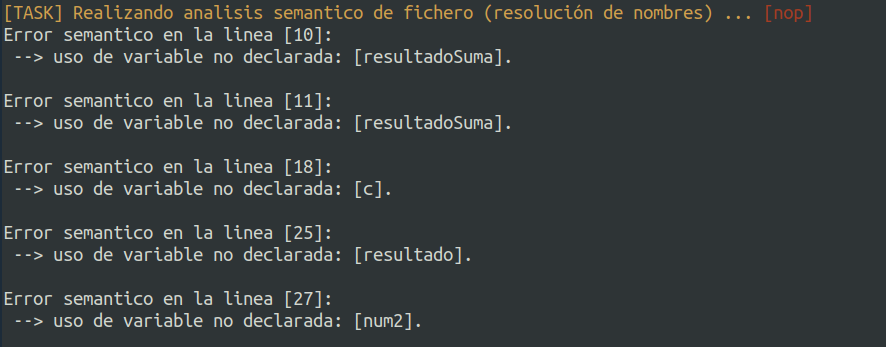
\includegraphics[width=\linewidth]{images/ejemplos/err_semantic/undef.png}
    \caption{Ejecución de programa: errores semánticos de no definición de variables.}
    \label{fig:lamportErrSemanticUndef_exec}
\end{figure}

\newpage
\subsection{Ejemplo 4: Errores semánticos: redefinición de variable}
\begin{lstlisting}[style=lamportStyle]
{Fichero: redef_variable.lmp}
{Autor: Daniel Perez Ruiz}
{Descripcion: Contiene un error semantico de tipo: redefinicion de variable}

program SumaEnteros
	var v1 : integer := 0;
	{ERROR: Redefinicion de variable}
	var v1 : integer;

process Main;
	var resultado : integer := 0;
	{ERROR: Redefinicion de variable}
	var resultado : char;
	{CORRECTO: este v1 esta en otro scope}
	var v1 : string := "hola";
begin
	{Invoca a la funcion para obtener el resultado}
	resultado := v1 + 2;
end
\end{lstlisting}
\begin{figure}[h]
\caption{Programa Lamport: errores semánticos de redefinición de variables.}
\label{fig:lamportErrSemanticRedef}
\end{figure}

\begin{figure}[h]
    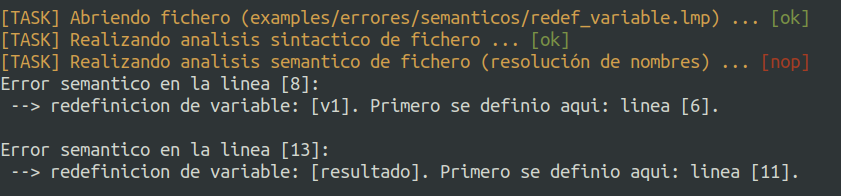
\includegraphics[width=\linewidth]{images/ejemplos/err_semantic/redef.png}
    \caption{Ejecución de programa: errores semánticos de no definición de variables.}
    \label{fig:lamportErrSemanticRedef_exec}
\end{figure}

\newpage
\subsection{Ejemplo 5: Errores semánticos: comprobación de tipos}
\begin{lstlisting}[style=lamportStyle]
{Fichero: typecheck_expressions.lmp}
{Autor: Daniel Perez Ruiz}
{Descripcion: Contiene errores semanticos de typechecking: expresiones}

program Sentencias
	var v1 : boolean := false;
	var v2 : string;
	var v3 : integer;
	
process Main;
	var v4 : real := 8.5;
	var resultado1 : integer;
	var resultado2 : real;
begin
	resultado1 := 1 + 3 * v3 - 1;
	{ERROR}
	resultado2 := v3 + 1.0 - 3;
	{ERROR}
	resultado1 := 1.0 - 10 / 2 + 7.5;
	{ERROR}
	resultado2 := 1 + 5 * 4;
	{ERROR}
	resultado2 := v2 + 3 / 2.5 - 1;
end
\end{lstlisting}
\begin{figure}[h]
\caption{Programa Lamport: errores semánticos en comprobación de tipos (expresiones).}
\label{fig:lamportErrSemanticTypecheck}
\end{figure}

\newpage
\begin{figure}[h]
    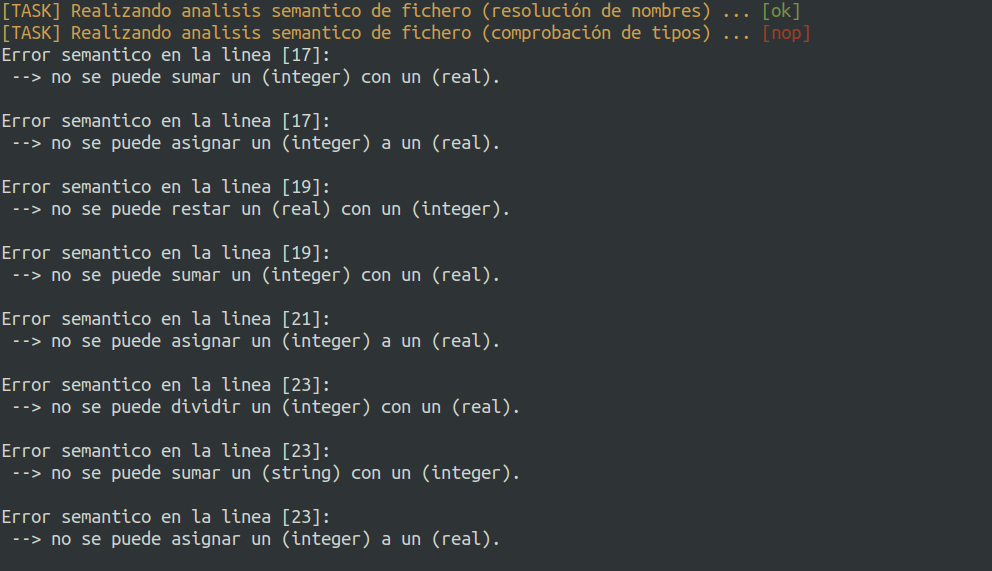
\includegraphics[width=\linewidth]{images/ejemplos/err_semantic/typecheck.png}
    \caption{Ejecución de programa: errores semánticos en comprobación de tipos (expresiones).}
    \label{fig:lamportErrSemanticTypecheck_exec}
\end{figure}

\newpage
\section{Ejemplos que lanzan excepciones}
Los siguientes ejemplos mostrados son correctos sintácticamente y semánticamente. Sin embargo, realizan operaciones no permitidas, y generan una excepción en la Máquina Virtual.

\subsection{Ejemplo 1: Excepción ZeroDivision}
\begin{lstlisting}[style=lamportStyle]
{Programa: zerodivision.lmp}
{Autor: Daniel Perez Ruiz}

program Operaciones
	var num1 : integer := 1;

process Main;
	var num2 : integer := 0;
	var resultado : integer;
begin
	{GENERA EXCEPCION EN LVM: Division zero}
	resultado := num1/num2;
end
\end{lstlisting}
\begin{figure}[h]
\caption{Programa Lamport: excepción ZeroDivision}
\label{fig:lamportExceptionZeroDivision}
\end{figure}

\begin{figure}[h]
    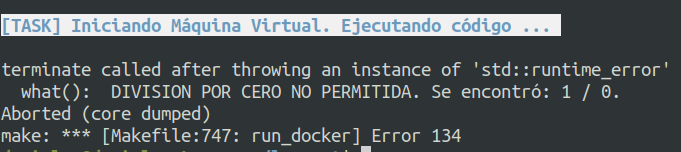
\includegraphics[width=\linewidth]{images/ejemplos/exceptions/zerodivision.png}
    \caption{Ejecución de programa: excepción ZeroDivision.}
    \label{fig:lamportExceptionZeroDivision_exec}
\end{figure}

\newpage
\subsection{Ejemplo 2: Excepción IndexOutOfBounds}
\begin{lstlisting}[style=lamportStyle]
{Programa: out_of_bounds.lmp}
{Autor: Daniel Perez Ruiz}

program Arrays
	var numeros : array [5] integer;

procedure negativeBound();
begin
	{EXCEPCION: Se intenta acceder a una posicion negativa de array}
	numeros[-2] := 2;
end

procedure excedBound();
begin
	{EXCEPCION: Se intenta acceder a una posicion negativa de array}
	numeros[6] := -2;
end

procedure printBadArray();
begin
	for i := 0 to 5 do
	begin
		print(numeros[i]);
	end
end
	
{INTERCAMBIE EL ORDEN DE EJECUCION PARA VER LAS EXCEPCIONES}
process main;
begin
	{EXCEPCION TIPO 2: Acceso a region fuera del limite superior}
	excedBound();
	
	{EXCEPCION TIPO 3: Recorrido en bucle que se sale de los limites}
	printBadArray();

	{EXCEPCION TIPO 1: Acceso negativo}
	negativeBound();
end
\end{lstlisting}
\begin{figure}[h]
\caption{Programa Lamport: excepción IndexOutOfBounds.}
\label{fig:lamportExceptionOutOfBounds}
\end{figure}

\newpage
\begin{figure}[h]
    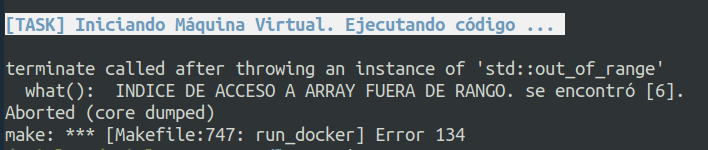
\includegraphics[width=\linewidth]{images/ejemplos/exceptions/out_of_bounds.png}
    \caption{Ejecución de programa: excepción IndexOutOfBounds.}
    \label{fig:lamportExceptionOutOfBounds_exec}
\end{figure}

\section{Ejemplos concurrentes}
Para finalizar, ha llegado el momento de verificar si se ha solucionado el problema que se planteó en el capítulo ~\ref{chapter:problema}, que es el de \textit{disponer de un lenguaje que permita simular sistemas concurrentes}. A continuación, se presenta una serie de ejemplos detallados que requiere de uso de concurrencia en el intérprete:

\subsection{Ejemplo 1: Múltiples procesos estáticos}
En este ejemplo se dispone de 3 procesos estáticos cuyo propósito es imprimir un mensaje por pantalla que consta de dos elementos: un mensaje de saludo seguido de una variable entera que actúa a modo de identificador de proceso. Estos mensajes están dentro de un bucle infinito, por lo que cada proceso se ejecutará indefinidamente:
\begin{lstlisting}[style=lamportStyle]
{Programa: race_condition.lmp}
{Autor: Daniel Perez Ruiz}

program Race

process P1;
	var id : integer := 1;
begin
	while true do
	begin
		print("te saluda el proceso: ",id);
	end
end

process P2;
	var id : integer := 2;
begin
	while true do
	begin
		print("te saluda el proceso: ",id);
	end
end

process P3;
	var id : integer := 3;
begin
	while true do
	begin
		print("te saluda el proceso: ",id);
	end
end
\end{lstlisting}
\begin{figure}[h]
\caption{Programa Lamport: múltiples procesos estáticos (race condition)}
\label{fig:lamportMultipleProcess}
\end{figure}

\begin{figure}[h]
    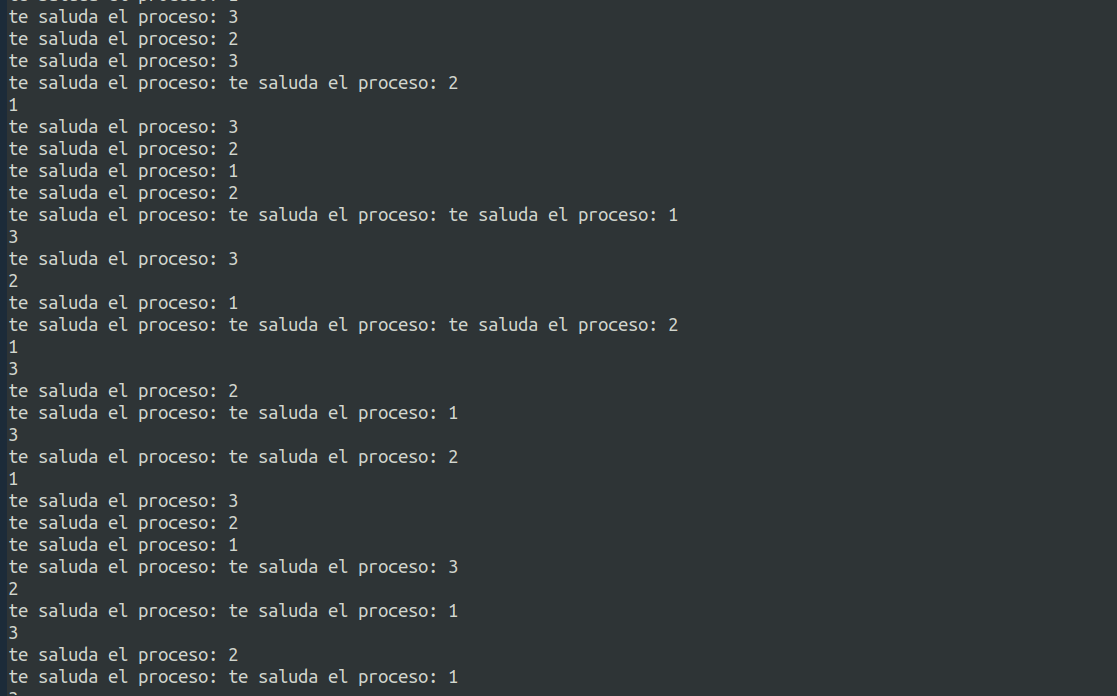
\includegraphics[width=\linewidth]{images/ejemplos/concurrentes/multiple_process.png}
    \caption{Ejecución de programa: múltiples procesos estáticos (race condition).}
    \label{fig:lamportMultipleProcess_exec}
\end{figure}

Se puede apreciar que efectivamente los tres procesos muestran mensajes. Sin embargo, en algunas ocasiones no se muestran correctamente porque se entrelazan las instrucciones de impresión de unos procesos con otros.

\newpage

\subsection{Ejemplo 2: Múltiples procesos estáticos (con sección atómica)}
Para solucionar el problema anterior, se puede introducir un bloque de secciones atómicas que contengan a las instrucciones de impresión en cada proceso, como se muestra a continuación:
\begin{lstlisting}[style=lamportStyle]
{Programa: atomic.lmp}
{Autor: Daniel Perez Ruiz}

program NotARace

process P1;
	var id : integer := 1;
begin
	while true do
	begin
		<< print("te saluda el proceso: ",id); >>
	end
end

process P2;
	var id : integer := 2;
begin
	while true do
	begin
		<< print("te saluda el proceso: ",id); >>
	end
end

process P3;
	var id : integer := 3;
begin
	while true do
	begin
		<< print("te saluda el proceso: ",id); >>
	end
end
\end{lstlisting}
\begin{figure}[h]
\caption{Programa Lamport: múltiples procesos estáticos (con sección atómica)}
\label{fig:lamportMultipleProcessAtomic}
\end{figure}

\newpage
\begin{figure}[h]
    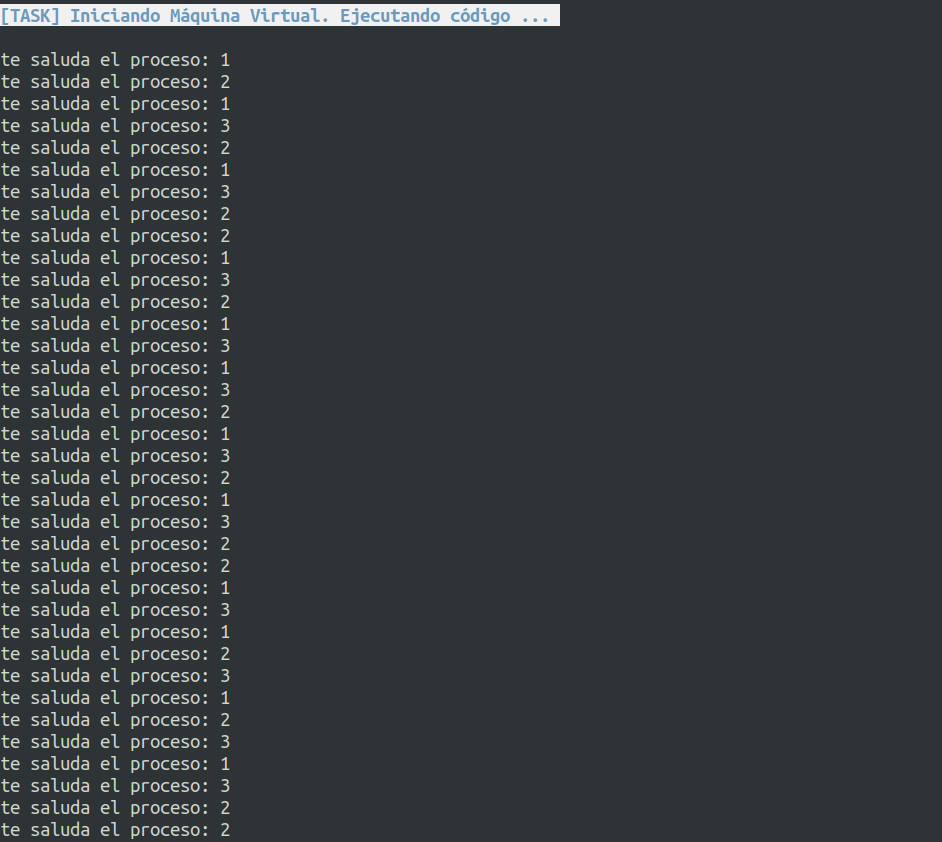
\includegraphics[width=\linewidth]{images/ejemplos/concurrentes/multiple_process_atomic.png}
    \caption{Ejecución de programa: múltiples procesos estáticos (con sección atómica)}
    \label{fig:lamportMultipleProcessAtomic_exec}
\end{figure}

Ahora, los tres procesos también muestran mensajes, pero se muestran ordenadamente debido a que, cuando una hebra entra en una sección atómica, se ejecutan todas las instrucciones que contiene hasta que termina. En este caso, se ejecutan 3 instrucciones dentro de cada sección atómica: saludo, índice y salto de línea.

\newpage
\subsection{Ejemplo 3: Vector de procesos estáticos}
En este ejemplo también se dispone de 3 procesos, pero han sido definidos mediante un vector indexado. Cada proceso dispone de su propio valor de índice, y lo utilizará para incrementar una variable compartida a los 3 procesos denominada \code{total}. El valor esperado final de la variable total es 6.
\begin{lstlisting}[style=lamportStyle]
{Programa: process_vector.lmp}
{Autor: Daniel Perez Ruiz}

program SumaIndice

	var total : integer := 0;

process VectorProc[index: 1..3];
begin
    total := total + index;
   	print("proceso (",index,") incrementa total a: ", total);
end
\end{lstlisting}
\begin{figure}[h]
\caption{Programa Lamport: vector de procesos estáticos (race condition).}
\label{fig:lamportProcessVector}
\end{figure}

\begin{figure}[h]
    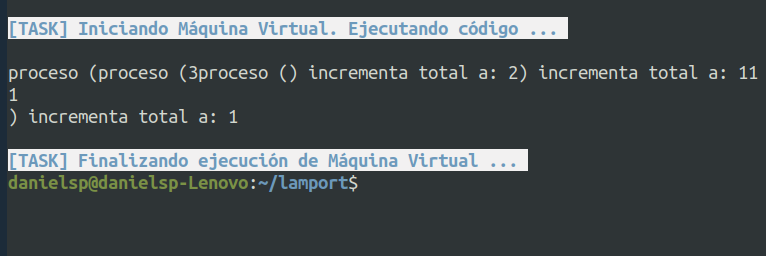
\includegraphics[width=\linewidth]{images/ejemplos/concurrentes/vector_process.png}
    \caption{Ejecución de programa: vector de procesos estáticos (race condition).}
    \label{fig:lamportProcessVector_exec}
\end{figure}

El resultado de esta ejecución es un caos tremendo debido a la concurrencia. No sólo en cuanto al contenido de los mensajes sino también en el resultado final que debería tener la variable global \code{total}.

\newpage
\subsection{Ejemplo 4: Vector de procesos estáticos (con atomic)}
Nuevamente, para solucionar el problema del ejemplo anterior es suficiente con definir una sección atómica que englobe a las dos instrucciones de los procesos.
\begin{lstlisting}[style=lamportStyle]
{Programa: process_vector_atomic.lmp}
{Autor: Daniel Perez Ruiz}

program SumaIndice

	var total : integer := 0;

process VectorProc[index: 1..3];
begin
    << total := total + index;
   	print("proceso (",index,") incrementa total a: ", total); >>
end
\end{lstlisting}
\begin{figure}[h]
\caption{Programa Lamport: vector de procesos estáticos (atómico).}
\label{fig:lamportProcessVectorAtomic}
\end{figure}

\begin{figure}[h]
    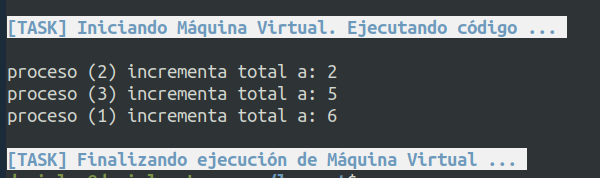
\includegraphics[width=\linewidth]{images/ejemplos/concurrentes/vector_process_atomic.png}
    \caption{Programa Lamport: vector de procesos estáticos (atómico).}
    \label{fig:lamportProcessVectorAtomic_exec}
\end{figure}

Aunque el orden de ejecución de los procesos puede ser diferente cada vez que se ejecute el programa, gracias a la sección atómica definida cada proceso muestra claramente el mensaje, y siempre el último mostrará que el resultado de la variable \code{total} es 6, como se esperaba.

\newpage
\subsection{Ejemplo 5: Bloque de instrucciones concurrentes (cobegin-coend)}
En el siguiente ejemplo se define una variable global denominada \code{x} cuyo valor inicial es 0. Después se define un proceso \code{Main} que contiene dos instrucciones de impresión y un bloque de instrucciones concurrentes. Puesto que al igual que en los otros ejemplos presentados aquí no se ha definido ningún mecanismo de sincronización, el resultado final de la variable \code{x} puede ser impredecible, aunque lo deseable sería que fuese 0.
\begin{lstlisting}[style=lamportStyle]
{Programa: cobegin.lmp}
{Autor: Daniel Perez Ruiz}

program Cobegin
	var x : integer := 0;
	
process Main;
begin
	print("iniciando bloque cobegin ...");

	cobegin
		x := x+1;
		x := x-1;
	coend
	
	print("x vale: ",x);
end
\end{lstlisting}
\begin{figure}[h]
\caption{Programa Lamport: bloque de instrucciones concurrentes cobegin-coend (race condition).}
\label{fig:lamportCobegin}
\end{figure}

\newpage

\begin{figure}[h]
    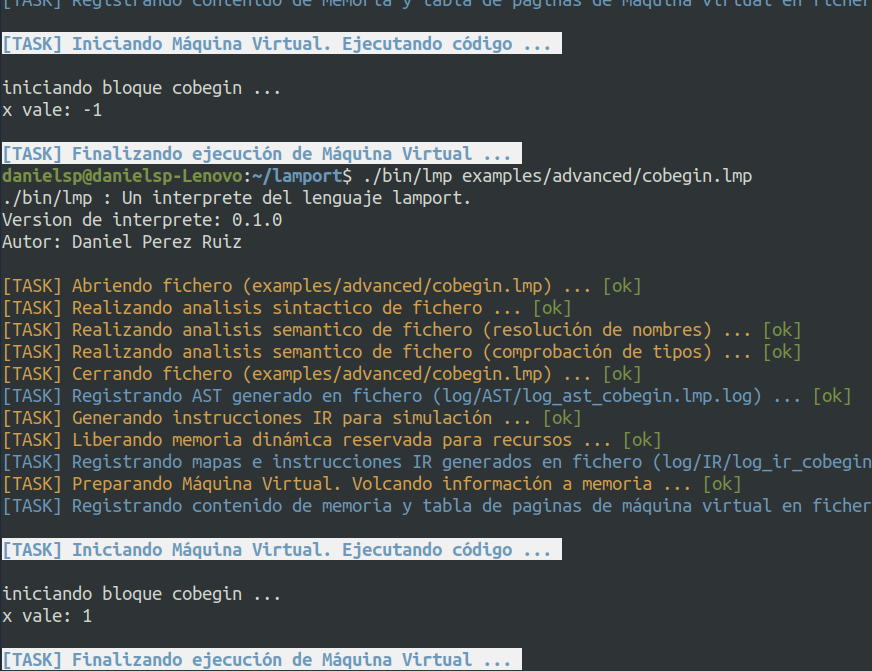
\includegraphics[width=\linewidth]{images/ejemplos/concurrentes/cobegin.png}
    \caption{Ejecución de programa: bloque de instrucciones concurrentes cobegin-coend (race condition).}
    \label{fig:lamportCobegin_exec}
\end{figure}

En estas dos ejecuciones del programa se ha obtenido un valor diferente: 1 y -1. De hecho, el conjunto de valores posibles para la variable \code{x} es: -1,0,1. Esto es evidentemente causado por el entrelazamiento de las hebras.

\vspace{0.5cm}
Notar además que, cuando se entra en un bloque cobegin, el proceso \code{Main} espera de manera implícita a que se ejecuten todas las hebras creadas dinámicamente para ejecutar todas las instrucciones que contiene.

\newpage
\subsection{Ejemplo 6: Bloque de instrucciones concurrentes (cobegin-coend) (con atomic)}
Si incluimos cada instrucción del bloque cobegin-coend en un bloque atómico, se soluciona el problema anteriormente mencionado.
\begin{lstlisting}[style=lamportStyle]
{Programa: cobegin.lmp}
{Autor: Daniel Perez Ruiz}

program Cobegin
	var x : integer := 0;
	
process Main;
begin
	print("iniciando bloque cobegin ...");

	cobegin
		<< x := x+1; >>
		<< x := x-1; >>
	coend
	
	print("x vale: ",x);
end
\end{lstlisting}
\begin{figure}[h]
\caption{Programa Lamport: bloque de instrucciones concurrentes cobegin-coend (atómico).}
\label{fig:lamportCobeginAtomic}
\end{figure}

\newpage

\begin{figure}[h]
    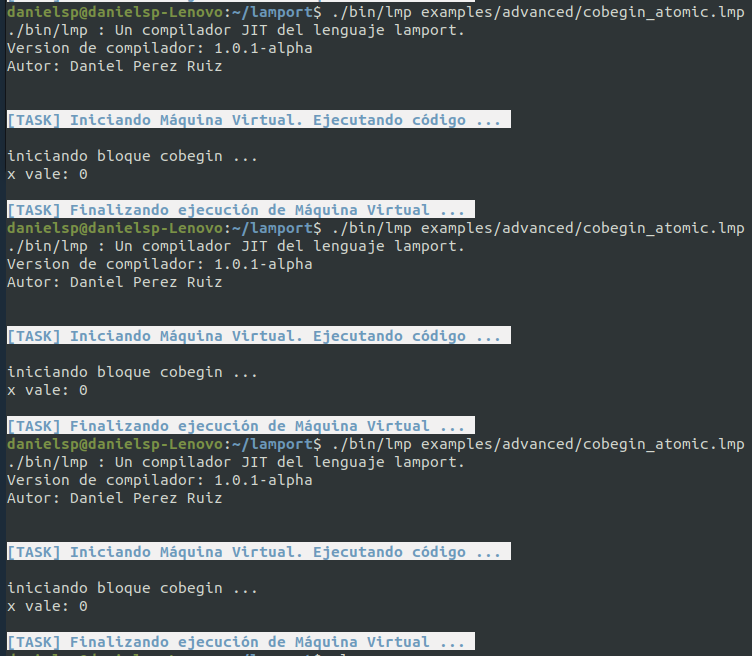
\includegraphics[width=\linewidth]{images/ejemplos/concurrentes/cobegin_atomic.png}
    \caption{Ejecución de programa: bloque de instrucciones concurrentes cobegin-coend (atómico).}
    \label{fig:lamportCobeginAtomic_exec}
\end{figure}

Ahora siempre que se ejecute este programa el resultado obtenido será 0, verificando así la buena sincronización de las hebras dentro de un bloque de instrucciones concurrentes de este tipo.

\newpage
\subsection{Ejemplo 7: Ejecución y sincronización de procedimientos concurrentes con fork-join}
En este ejemplo disponemos de una variable global \code{x} y dos procedimientos que hacen dos tareas diferentes. Uno incrementa la variable \code{x} unas 100 veces, y otro lo decrementa unas 20 veces. El resultado final que debería tener la variable es \code{x = 80}. Ejecutándolo secuencialmente, se verifica sin problema, pero el objetivo de este programa es ejecutar sendos procedimientos concurrentemente. 

\vspace{0.5cm}

El proceso \code{Main} indica a Increment que se ejecute concurrentemente con la llamada que realiza después a decrement, utilizando la sentencia \code{fork}. Con la sentencia \code{join}, la hebra \code{Main} se bloquea esperando a que \code{Increment()} termine su ejecución.
\begin{lstlisting}[style=lamportStyle]
{Programa: fork_join.lmp}
{Autor: Daniel Perez Ruiz}

program Fork;
	var x : integer := 0;

procedure Increment();
begin
	for i := 1 to 100 do
	begin
		x := x+1;
	end
	
	print("fin de increment");
end

procedure Decrement();
begin
	for j := 1 to 20 do
	begin
		x := x-1;
	end
	
	print("fin de decrement");
end

process Main;
begin
	print("Realizando fork...");
	fork Increment;
	Decrement();
	join;
	
	print("x vale: ",x);
	
	
	if(x == 80) then
	begin
		print("Se ha obtenido 80, el valor esperado");
	end
	else
	begin
		print("No se ha obtenido 80.");
	end
end
\end{lstlisting}
\begin{figure}[h]
\caption{Programa Lamport: creación y sincronización de hebras dinámicas con fork-join.}
\label{fig:lamportForkJoin}
\end{figure}

\newpage

\begin{figure}[h]
    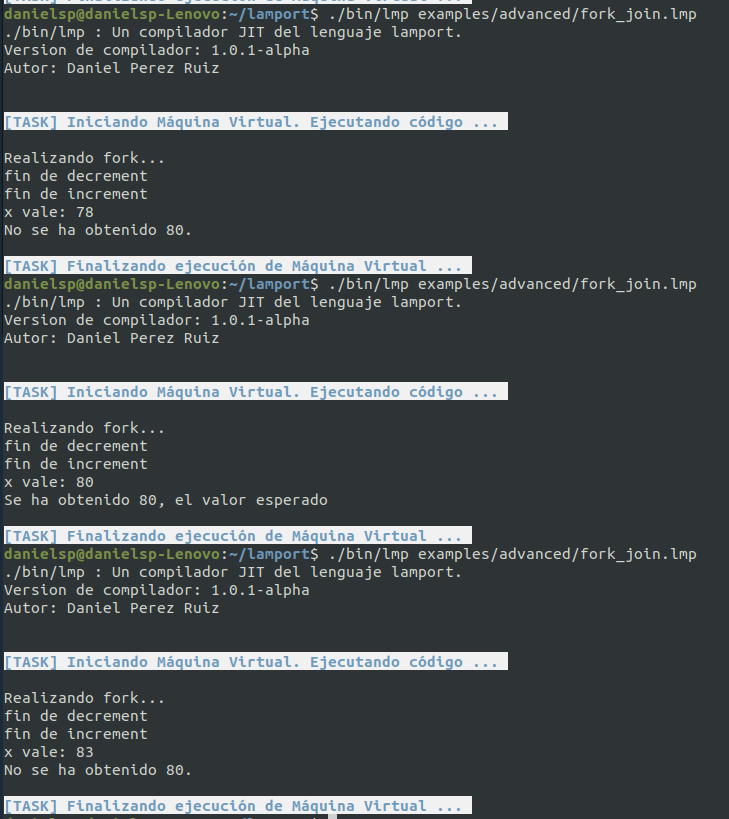
\includegraphics[width=\linewidth]{images/ejemplos/concurrentes/fork_join.png}
    \caption{Ejecución de programa: creación y sincronización de hebras dinámicas con fork-join.}
    \label{fig:lamportForkJoin_exec}
\end{figure}

Se observa que la sincronización de Increment con la hebra principal Main se realiza adecuadamente, pues los mensajes que se escribieron después de join se ejecutan sí y sólo sí cuando este procedimiento ha terminado. Sin embargo, se vuelve a apreciar que en dos ejecuciones del programa no hay el resultado esperado, obteniendo dos resultados diferentes.

\newpage
Si las instrucciones de las líneas 11 y 21 se engloban dentro de una sección atómica, el resultado de la ejecución del programa es el siguiente, donde siempre se conseguirá el valor deseado de la variable \code{x}.

\begin{figure}[h]
    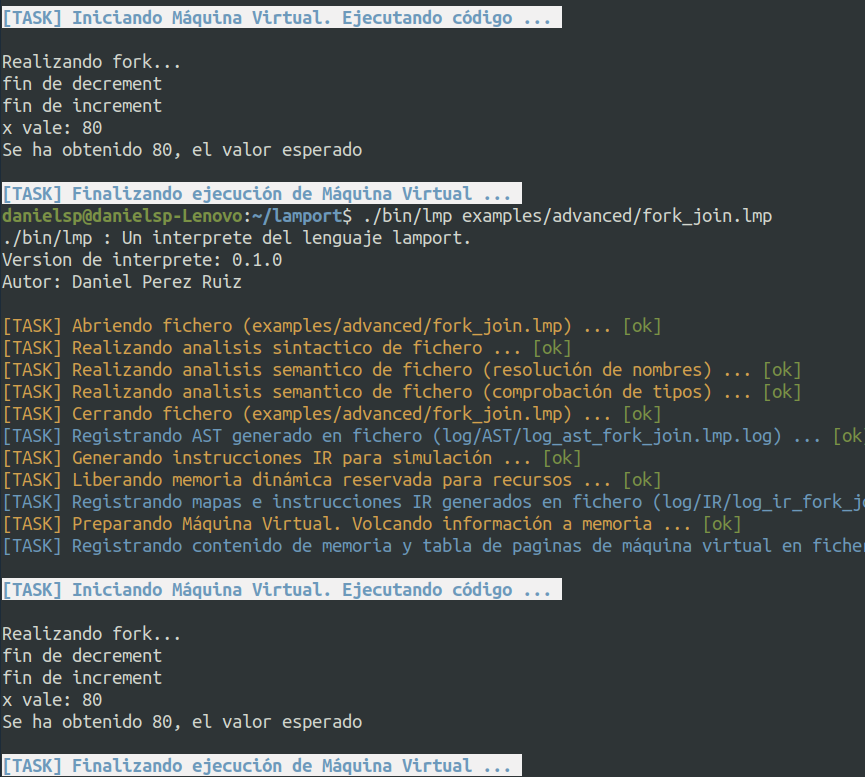
\includegraphics[width=\linewidth]{images/ejemplos/concurrentes/fork_join_atomic.png}
    \caption{Ejecución de programa: creación y sincronización de hebras dinámicas con fork-join (atómico).}
    \label{fig:lamportForkJoinAtomic_exec}
\end{figure}

\newpage
Finalmente, queda preguntarse qué sucede si se elimina la instrucción \code{join} (línea 32) que es quien sincroniza al proceso \code{Main} con su hija. Lo más probable es que lo que ocurra sea que la hebra principal termine antes que su hija, un comportamiento poco deseado y que se aprecia a continuación:

\begin{figure}[h]
    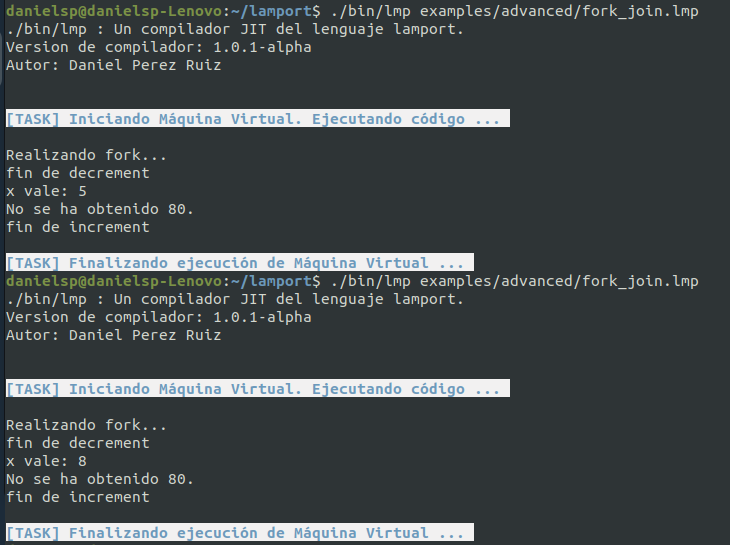
\includegraphics[width=\linewidth]{images/ejemplos/concurrentes/fork_without_join.png}
    \caption{Ejecución de programa: creación y sincronización de hebras dinámicas con fork (sin join).}
    \label{fig:lamportForkWithoutJoin_exec}
\end{figure}

Se observa que los mensajes de impresión después de la llamada a los procedimientos se muestran antes de que Increment notifique que ha terminado.

\newpage
\subsection{Ejemplo 8: Sincronización de procedimientos concurrentes con semáforos}
Este ejemplo es bastante parecido al anterior, con la salvedad de que se tiene otra forma diferente de sincronizar los procedimientos \code{Increment} y \code{Decrement}. Se observa un semáforo denominado \code{sem} y cuyo valor de inicio es 1.

\vspace{0.5cm}

Un semáforo es una herramienta de sincronización utilizada en la programación concurrente para controlar el acceso a un recurso compartido. Funciona como un contador, y sus operaciones fundamentales son \code{WAIT} (o también llamada \textit{P}) y \code{SIGNAL} (o \textit{V}). El \code{WAIT} disminuye el contador y, si este es negativo, bloquea el proceso; mientras que el \code{SIGNAL} incrementa el contador y, si hay procesos bloqueados, permite que uno de ellos continue su ejecución. De esta manera, los semáforos pueden garantizar que ciertas secciones de código no sean ejecutadas por más de un proceso a la vez, evitando condiciones de carrera y otros problemas relacionados con la concurrencia.

\begin{lstlisting}[style=lamportStyle]
{Programa: semaphore.lmp}
{Autor: Daniel Perez Ruiz}
program Semaphore;
    var x : integer := 2;
    var sem : semaphore := 1;

procedure Increment();
begin
    for i := 1 to 5 do
    begin
        WAIT sem;
        print("Incrementando x, que vale ahora: ", x);
        x := x + 1;
        SIGNAL sem;
    end
end

procedure Decrement();
begin
    for i := 1 to 5 do
    begin
        WAIT sem;
        print("Decrementando x, que vale ahora: ", x);
        x := x - 1;
        SIGNAL sem;
    end
end

process Main;
begin
    fork Increment;
    fork Decrement;
    join;
    print("x vale: ", x);
end
\end{lstlisting}
\begin{figure}[h]
\caption{Programa Lamport: sincronización de procesos con semáforo.}
\label{fig:lamportSemaphore}
\end{figure}

\begin{figure}[h]
    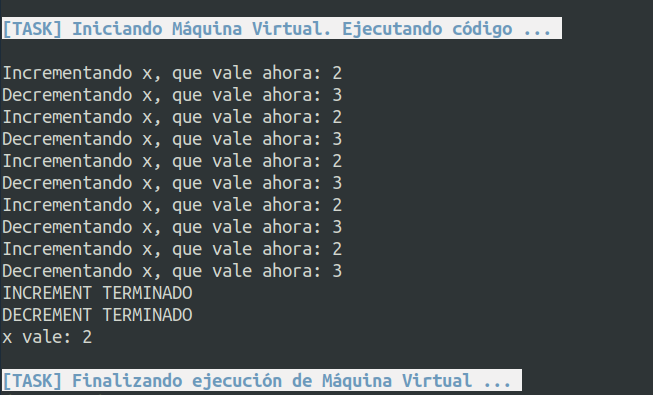
\includegraphics[width=\linewidth]{images/ejemplos/concurrentes/semaphore.png}
    \caption{Ejecución de programa: sincronización de procesos con semáforo.}
    \label{fig:lamportSemaphore_exec}
\end{figure}

En esta ejecución se observa que cada procedimiento modifica una única vez el valor de la variable global, dando como resultado final 2, que era el valor esperado tras incrementar y decrementar 1 unidad el número, el mismo número de veces.

	% Conclusiones
	\chapter{\textbf{Conclusiones y trabajos futuros}}

\section{Conclusiones}
Este proyecto ha abarcado dos áreas fundamentales relacionadas con los sistemas concurrentes y distribuidos. Primero, se llevó a cabo un estudio exhaustivo de los sistemas concurrentes, centrando la atención en una especificación formal como la propuesta por Leslie Lamport en su Lógica Temporal de Acciones (TLA). Este análisis detallado no solo proporcionó una base teórica sólida para entender la complejidad inherente a estos sistemas, sino que también destacó la importancia de una especificación rigurosa para su correcto diseño y verificación, a través del formalismo matemático.

En segundo lugar, se adoptó un enfoque práctico mediante el desarrollo de un intérprete para un lenguaje de programación diseñado específicamente para simular sistemas concurrentes y distribuidos. Este lenguaje se basó en el pseudocódigo utilizado en la asignatura ``Sistemas Concurrentes y Distribuidos'', permitiendo así una mayor accesibilidad y comprensión para aquellos familiarizados con el curso. La implementación de este intérprete se realizó siguiendo una metodología de desarrollo ágil, lo que facilitó un proceso de desarrollo iterativo y adaptable.

Durante este proceso, se utilizaron herramientas avanzadas de programación, incluyendo analizadores léxicos y sintácticos, y se aprovecharon las capacidades de los lenguajes C y C++ para asegurar un rendimiento óptimo y una integración efectiva. Esta combinación de teoría y práctica no solo ha enriquecido la comprensión de los sistemas concurrentes y distribuidos, sino que también ha proporcionado una herramienta valiosa para su estudio y simulación.

Al concluir este proyecto, se ha logrado un balance entre la teoría formal y la aplicación práctica, proporcionando una perspectiva integral de los sistemas concurrentes y distribuidos. Este trabajo no solo sirve como un recurso educativo para aquellos que buscan profundizar en este campo, sino que también sienta las bases para futuras investigaciones y desarrollos en esta área tan dinámica y desafiante de la informática.

\section{Trabajos futuros}
Desarrollar un intérprete completo para dar vida a un nuevo lenguaje de programación es cuanto menos desafiante, además teniendo en cuenta los cortos plazos de tiempo en los que se han desarrollado. Puesto que el software siempre está en continua evolución y en continua obsolescencia, hay algunos aspectos que se pueden mejorar y nuevas que desarrollar, citadas a continuación:

\begin{itemize}
    \item \textbf{SAAS (Software As A Service)}: Con el intérprete ya dockerizado, una prometedora dirección futura para este proyecto es su desarrollo y lanzamiento como Software as a Service (SaaS). Esta transición a una plataforma basada en la nube no solo facilitaría un acceso más amplio y flexible al intérprete, sino que también permitiría una gestión más eficiente y la implementación rápida de actualizaciones y mejoras. Al ofrecer el intérprete como un servicio en la nube, podríamos expandir significativamente su alcance y utilidad, proporcionando una herramienta valiosa y accesible para una audiencia global interesada en la simulación y el estudio de sistemas concurrentes y distribuidos.
    \item \textbf{Nuevos mecanismos de sincronización y ampliación de la gramática}: De forma nativa el intérprete permite definir semáforos como mecanismo de sincronización de hebras, por lo que quizá estaría bien considerar otras como ``Monitores''. También, puede considerarse ampliar la gramática de Lamport permitiendo nuevos constructos que faciliten el uso por parte del usuario.
    \item \textbf{Reimplementación de intérprete en C++}: En este proyecto se utilizó C y C++ como lenguajes de desarrollo del intérprete, dejando C para la parte más cercana a la fase de análisis de código (léxico, sintáctico y semántico). Aunque C es un lenguaje muy versátil a día de hoy, su sucesor C++ implementa características más seguras, en lo que concierne a gestión de memoria dinámica vía punteros. Por otra parte, su sintaxis orientada a objetos y sus múltiples bibliotecas estándar hace que la definición y/o uso de estructuras de datos sea más directa que en C, y como Flex y Bison permiten generar analizadores para este lenguaje, quizá sería conveniente reimplementar todos esos módulos con este lenguaje, garantizando más seguridad y claridad.
    \item \textbf{Gestión de errores sintácticos uniforme}: Se podría mejorar la gestión actual de los errores sintácticos por parte de Bison, definiendo unas reglas de producción más granulares y específicas, incluso teniendo en cuenta patrones incorrectos debido a tokens que no debían estar ahí.
    \item \textbf{Habilitar expresiones en definición de arrays}: Gestionar la memoria en tiempo de ejecución es una tarea ardua si las implementaciones deben hacerse desde cero, y es por eso por lo que la gramática actual, aunque contemple cualquier tipo de expresión para la declaración de arrays, se considera semánticamente incorrecta la declaración si dicha expresión no contiene exactamente un literal entero. Es por ello por lo que dentro de la memoria de la máquina virtual se podría considerar un heap que permita obtener el tamaño de los arrays en tiempo de ejecución.
    \item \textbf{Simulación realista de la asignación de los registros}: Con la estrategia actual la simulación que hace la máquina virtual es menos realista que lo que se hace en una máquina convencional. Se podría considerar cambiar esta mecánica de decisión de registros a la hora de generar las instrucciones de la representación intermedia, comprobando la vivacidad de los registros.
\end{itemize}

Para concluir, este proyecto no solo representa un paso significativo en la simulación y estudio de sistemas concurrentes y distribuidos, sino que también establece una sólida base para futuras innovaciones y mejoras. Con estas vías futuras, el proyecto está bien posicionado para adaptarse y evolucionar, manteniéndose relevante y útil en un campo que está en constante cambio y crecimiento.

	% Trabajos futuros


	
	\newpage
        \nocite{*}
	\bibliography{bibliografia}
	\bibliographystyle{plain}
	
\end{document}

